\documentclass[12pt,a4paper]{article}

% ---- Packages ----
\usepackage[margin=1in,headheight=15pt]{geometry}
\usepackage{amsmath,amssymb,amsthm}
\usepackage{mathtools}
\usepackage{enumitem}
\usepackage[hypertexnames=false]{hyperref}
\usepackage{cleveref}
\usepackage{setspace}
\usepackage{fancyhdr}
\usepackage{titlesec}
\usepackage{tikz}
\usepackage{pgfplots}
\usepackage{algorithm}
\usepackage{float}
\usepackage{graphicx}
\usepackage{algpseudocode}
\pgfplotsset{compat=1.18}
\usetikzlibrary{arrows.meta,decorations.markings}

% ---- Theorem environments ----
\theoremstyle{definition}
\newtheorem{definition}{Definition}[section]
\newtheorem{assumption}{Assumption}[section]
\newtheorem{example}{Example}[section]
\theoremstyle{plain}
\newtheorem{theorem}{Theorem}[section]
\newtheorem{proposition}{Proposition}[section]
\newtheorem{lemma}{Lemma}[section]
\newtheorem{corollary}{Corollary}[section]
\theoremstyle{remark}
\newtheorem{remark}{Remark}[section]

% ---- Shortcuts ----
\newcommand{\R}{\mathbb{R}}
\newcommand{\E}{\mathbb{E}}
\newcommand{\zbar}{\bar{z}}
% Clean lower bound: use subscript notation instead of \underline which is ugly in integral limits
\newcommand{\zlow}{z_{\scriptscriptstyle 0}}
\newcommand{\calU}{\mathcal{U}}
\newcommand{\calZ}{\mathcal{Z}}
\newcommand{\calL}{\mathcal{L}}
\newcommand{\calA}{\mathcal{A}}
\newcommand{\calM}{\mathcal{M}}
\newcommand{\calR}{\mathcal{R}}
\newcommand{\calY}{\mathcal{Y}}
\DeclareMathOperator*{\argmax}{arg\,max}

% ---- Header ----
\pagestyle{fancy}
\fancyhf{}
\rhead{Optimal Nonlinear Taxation}
\lhead{Lecture Notes}
\cfoot{\thepage}

% ---- Title ----
\title{\textbf{Optimal Nonlinear Income Taxation} \\ \large Lecture Notes}
\author{}
\date{}

\begin{document}
\maketitle
\thispagestyle{fancy}

\tableofcontents
\newpage

%==========================================================================
\section{The Environment}
\label{sec:environment}
%==========================================================================

\subsection{Households}

There is a continuum of households indexed by their productivity type $z \in \calZ = [\zlow, \zbar]$, distributed according to a cumulative distribution function $F(z)$ with density $f(z) > 0$ on $\calZ$.

\begin{remark}[Bounded vs.\ unbounded support]
\label{rem:support}
The notation $\calZ = [\zlow, \zbar]$ allows $\zbar = \infty$: the support may be unbounded above. Much of the analysis in Sections~\ref{sec:environment}--\ref{sec:mechanism} is stated for a generic interval $[\zlow, \zbar]$ and applies in either case. The distinction matters for the optimal tax schedule at the top of the distribution: with bounded support, the marginal tax rate is zero at $\zbar$ (Section~\ref{sec:special}); with unbounded support and a Pareto tail, the limiting marginal tax rate is generally positive (the Diamond--Saez formula, also in Section~\ref{sec:special}).
\end{remark}

Each household of type $z$ has preferences over consumption $c$ and labor supply $n$, represented by the utility function $U(c, n; z)$. We suppress the explicit dependence on $z$ when it enters only through the budget constraint (as below), and write $U(c,n)$.

A household of type $z$ produces output
\[
  y(z) = z \, n(z),
\]
so that $z$ is the marginal product of labor. For given output $y$, the labor required is $n = y/z$.

\begin{assumption}[Regularity of preferences]
\label{as:concavity}
The utility function $U(c,n)$ is twice continuously differentiable and strictly concave:
\[
  U_{cc} < 0, \qquad U_{cc} U_{nn} - U_{cn}^2 > 0.
\]
\end{assumption}

\begin{assumption}[Normality]
\label{as:normal}
Both consumption and leisure are normal goods. That is, when a household solves
\[
  \max_n \; U(zn + I, \, n)
\]
for exogenous nonlabor income $I$, we have $c'(I) > 0$ and $n'(I) < 0$.
\end{assumption}

We verify Assumption~\ref{as:normal} explicitly. The first-order condition of the household problem $\max_n U(zn+I, n)$ is
\[
  z \, U_c(zn+I, n) + U_n(zn+I, n) = 0.
\]
Totally differentiating with respect to $I$:
\[
  z \, U_{cc}(z n'(I) + 1) + z \, U_{cn} \, n'(I) + U_{nc}(z n'(I) + 1) + U_{nn} \, n'(I) = 0.
\]
Collecting terms in $n'(I)$:
\[
  \bigl[ z^2 U_{cc} + 2z U_{cn} + U_{nn} \bigr] n'(I) = -\bigl[ z U_{cc} + U_{nc} \bigr].
\]
Hence
\begin{equation}
\label{eq:income_effect_n}
  n'(I) = -\frac{z U_{cc} + U_{nc}}{z^2 U_{cc} + 2z U_{cn} + U_{nn}},
\end{equation}
and
\begin{equation}
\label{eq:income_effect_c}
  c'(I) = z n'(I) + 1 = \frac{z U_{cn} + U_{nn}}{z^2 U_{cc} + 2z U_{cn} + U_{nn}}.
\end{equation}
The denominator is the quadratic form
\[
  (z, 1)
  \begin{pmatrix} U_{cc} & U_{cn} \\ U_{cn} & U_{nn} \end{pmatrix}
  \begin{pmatrix} z \\ 1 \end{pmatrix}
  = z^2 U_{cc} + 2z U_{cn} + U_{nn} < 0,
\]
which is strictly negative by the strict concavity of $U$ (Assumption~\ref{as:concavity} implies the Hessian is negative definite). Therefore, the normality conditions $n'(I) < 0$ and $c'(I) > 0$ require
\begin{equation}
\label{eq:normality_conditions}
  z U_{cc} + U_{nc} < 0 \qquad \text{(leisure is normal)}, \qquad
  z U_{cn} + U_{nn} < 0 \qquad \text{(consumption is normal)}.
\end{equation}

\subsection{Government}

The government has an exogenous revenue requirement $B \geq 0$. It must design a tax-and-transfer system subject to the economy-wide resource constraint
\begin{equation}
\label{eq:resource}
  \int_{\zlow}^{\zbar} \bigl[ y(z) - c(z) \bigr] f(z) \, dz \geq B.
\end{equation}
The government evaluates outcomes using a social welfare function
\[
  \int_{\zlow}^{\zbar} \psi(z) \, U(c(z), n(z)) \, f(z) \, dz,
\]
where $\psi(z) \geq 0$ are Pareto weights with $\int \psi(z) f(z) \, dz = 1$. A preference for redistribution is captured by $\psi(z)$ declining in $z$: the planner values utility gains to low types more than to high types.

\subsection{First-best benchmark}

If the government could observe each household's type $z$ directly, it would solve
\[
  \max_{c(\cdot), y(\cdot)} \int_{\zlow}^{\zbar} \psi(z) \, U\!\left(c(z), \frac{y(z)}{z}\right) f(z) \, dz
  \quad \text{s.t.} \quad
  \int_{\zlow}^{\zbar} \bigl[ y(z) - c(z) \bigr] f(z) \, dz \geq B,
\]
where $\psi(z)$ is the Pareto weight on type $z$. With Lagrange multiplier $\mu$ on the resource constraint, the first-order conditions are
\begin{align}
  [c(z)]: & \quad \psi(z) \, U_c\!\left(c(z), \frac{y(z)}{z}\right) = \mu, \label{eq:fb_c} \\[4pt]
  [y(z)]: & \quad \psi(z) \, U_n\!\left(c(z), \frac{y(z)}{z}\right) \frac{1}{z} = -\mu. \label{eq:fb_y}
\end{align}
Dividing \eqref{eq:fb_y} by \eqref{eq:fb_c}, the Pareto weights cancel and we obtain
\begin{equation}
\label{eq:fb_wedge}
  -\frac{U_n\!\left(c(z), \frac{y(z)}{z}\right)}{z \, U_c\!\left(c(z), \frac{y(z)}{z}\right)} = 1.
\end{equation}
The left-hand side is the marginal rate of substitution between output and consumption, which equals the marginal rate of transformation (unity). \emph{There are no distortions at the first best}: the implicit marginal tax rate is zero for all types. This holds for \emph{any} Pareto weights $\psi(z)$, not just the utilitarian case---at the first best, the planner can redistribute via lump-sum transfers without distorting the labor-leisure margin.

The extent of redistribution, however, does depend on $\psi(z)$. The first-order condition \eqref{eq:fb_c} gives $U_c(c(z), y(z)/z) = \mu / \psi(z)$: marginal utilities of consumption are inversely proportional to Pareto weights. Under a utilitarian objective with $\psi(z) = 1$ for all $z$, this equalizes $U_c$ across all types---the planner redistributes until marginal utilities of consumption are equalized.



\begin{remark}[Utility gradient at the first best (utilitarian case)]
Under utilitarian weights $\psi(z) = 1$, the FOCs \eqref{eq:fb_c}--\eqref{eq:fb_y} become $U_c = \mu$ and $-U_n/z = \mu$. Differentiating $U_c = \mu$ (constant) with respect to $z$:
\[
  U_{cc} \, c'(z) + U_{cn} \frac{y'(z) z - y(z)}{z^2} = 0.
\]
Similarly, differentiating $-U_n/z = \mu$:
\[
  \frac{1}{z^2} U_n - \frac{1}{z} U_{nc} \, c'(z) - \frac{1}{z} U_{nn} \frac{y'(z) z - y(z)}{z^2} = 0.
\]
Solving these two equations simultaneously:
\begin{align*}
  c'(z) &= -\frac{1}{z} \frac{U_n \, U_{cn}}{U_{nn} U_{cc} - U_{cn}^2}, \\[4pt]
  \frac{y'(z) z - y(z)}{z^2} &= \frac{1}{z} \frac{U_n \, U_{cc}}{U_{nn} U_{cc} - U_{cn}^2}.
\end{align*}
The utility gradient is then
\begin{align}
  \frac{dU}{dz}
  &= U_c \, c'(z) + U_n \frac{y'(z)z - y(z)}{z^2} \notag \\
  &= \frac{1}{z} \bigl[ U_n U_{cc} - U_c U_{cn} \bigr] \frac{U_n}{U_{nn} U_{cc} - U_{cn}^2} \notag \\
  &= -\frac{\mu}{z}
    \underbrace{\bigl[ z U_{cc} + U_{cn} \bigr]}_{< 0 \text{ (leisure normal)}}
    \underbrace{\frac{U_n}{U_{nn} U_{cc} - U_{cn}^2}}_{< 0} < 0.
  \label{eq:fb_utility_gradient}
\end{align}
Under utilitarian weights, higher-productivity households have \emph{lower} utility at the first best: the planner equalizes marginal utilities ($U_c = \mu$ for all $z$) and makes more productive types work harder, so they do not enjoy the fruits of their higher productivity. With general Pareto weights $\psi(z)$, the gradient depends on $\psi'(z)$ as well, and the sign can go either way.

\end{remark}
%==========================================================================
\section{The Nonlinear Income Tax Problem}
\label{sec:tax_problem}
%==========================================================================

The first-best allocation from Section~\ref{sec:environment} requires the government to observe each household's type $z$ directly. In practice, the government observes only income $y = zn$, not the decomposition into productivity $z$ and labor $n$ separately. The government's instrument is therefore a \emph{nonlinear income tax schedule} $T: \R_+ \to \R$, mapping pre-tax income $y$ to a tax payment $T(y)$ (with $T(y) < 0$ representing a transfer).

\subsection{The household's problem given $T$}

Facing a tax schedule $T(\cdot)$, a household of type $z$ solves
\begin{equation}
\label{eq:HH_problem}
  \max_{y \geq 0} \; U\!\left( y - T(y), \; \frac{y}{z} \right).
\end{equation}
Let $y^*(z; T)$ denote the solution and define the induced allocation
\[
  y(z) = y^*(z; T), \qquad c(z) = y(z) - T(y(z)).
\]
If $T$ is differentiable at $y(z)$ and $y(z) > 0$, the first-order condition is
\begin{equation}
\label{eq:HH_foc_tax}
  \bigl[1 - T'(y(z))\bigr] \, U_c\!\left(c(z), \frac{y(z)}{z}\right) + \frac{1}{z} \, U_n\!\left(c(z), \frac{y(z)}{z}\right) = 0,
\end{equation}
which says the marginal rate of substitution between output and consumption equals the net-of-tax return:
\[
  -\frac{U_n(c, y/z)}{z \, U_c(c, y/z)} = 1 - T'(y).
\]

\subsection{The government's problem over tax functions}

The government chooses $T(\cdot)$ to maximize social welfare subject to the resource constraint, \emph{taking into account} that households optimize in response:
\begin{equation}
\label{eq:govt_tax}
\begin{split}
  \max_{T(\cdot)} \quad & \int_{\zlow}^{\zbar} \psi(z) \, U\!\left( y^*(z;T) - T(y^*(z;T)), \; \frac{y^*(z;T)}{z} \right) f(z) \, dz \\
  \text{s.t.} \quad & \int_{\zlow}^{\zbar} T(y^*(z;T)) \, f(z) \, dz \geq B.
\end{split}
\end{equation}

This is a difficult problem for two reasons:
\begin{enumerate}[label=(\roman*)]
  \item \textbf{Infinite-dimensional control.} The choice variable is an entire function $T: \R_+ \to \R$, not a finite-dimensional parameter.
  \item \textbf{Implicit dependence on $T$.} The mapping from the tax schedule to household behavior, $z \mapsto y^*(z; T)$, is determined implicitly through each household's optimization problem \eqref{eq:HH_problem}. Small changes in $T$ can produce discontinuous jumps in behavior (e.g., when bunching occurs), and the map $T \mapsto y^*(\cdot\,; T)$ is generally non-smooth.
\end{enumerate}

\subsection{From tax functions to allocations: the taxation principle}

The \emph{taxation principle} (a special case of the revelation principle) provides a way around these difficulties. It establishes an equivalence between two formulations of the problem.

\begin{definition}[Incentive compatibility]
\label{def:IC}
An allocation $\{c(z), y(z)\}_{z \in \calZ}$ is \emph{incentive compatible} (IC) if no type gains by mimicking another: for all $z, \tilde z \in \calZ$,
\[
  U\!\left(c(z), \frac{y(z)}{z}\right) \geq U\!\left(c(\tilde z), \frac{y(\tilde z)}{z}\right).
\]
\end{definition}

\begin{proposition}[Taxation principle]
\label{prop:taxation}
An allocation $\{c(z), y(z)\}_{z \in \calZ}$ can be implemented by some nonlinear tax schedule $T(\cdot)$ if and only if it is incentive compatible (Definition~\ref{def:IC}) and resource feasible \eqref{eq:resource}.
\end{proposition}

The key insight is the direction from allocations back to taxes: given any incentive-compatible allocation $\{c(z), y(z)\}$, one can construct a tax schedule $T(y) = y - c(z)$ for $y$ in the range of $y(\cdot)$, extended appropriately off the equilibrium path, that implements the allocation. This means instead of optimizing over the space of tax functions, the planner can equivalently optimize over the space of incentive-compatible allocations---a more tractable problem.

%==========================================================================
\section{The Mechanism Design Formulation}
\label{sec:mechanism}
%==========================================================================

By the taxation principle (Proposition~\ref{prop:taxation}), we can optimize over incentive-compatible allocations $\{c(z), y(z)\}$ rather than tax functions. In this section we characterize the IC constraint (Definition~\ref{def:IC}) and show that, under a single-crossing condition, it reduces to a local envelope condition plus monotonicity.

\subsection{The announcement problem and local IC}

A household of true type $z$ facing the mechanism $\{c(\cdot), y(\cdot)\}$ chooses which type $\tilde z$ to announce:
\begin{equation}
\label{eq:announcement}
  \max_{\tilde z} \; U\!\left( c(\tilde z), \frac{y(\tilde z)}{z} \right).
\end{equation}
At an IC allocation, truth-telling ($\tilde z = z$) is optimal. The first-order condition at $\tilde z = z$ gives the \emph{local} IC condition:
\begin{equation}
\label{eq:local_IC_FOC}
  U_c\!\left( c(z), \frac{y(z)}{z} \right) c'(z)
  + U_n\!\left( c(z), \frac{y(z)}{z} \right) \frac{y'(z)}{z} = 0.
\end{equation}

\subsection{The envelope condition (local incentive compatibility)}

Define the value function of the announcement problem:
\[
  V(z) = \max_{\tilde z} \; U\!\left( c(\tilde z), \frac{y(\tilde z)}{z} \right).
\]
At an incentive-compatible allocation, $V(z) = U(c(z), y(z)/z) \equiv \calU(z)$. By the envelope theorem, we differentiate with respect to $z$ \emph{only through the place where $z$ appears directly} (i.e., in $y(\tilde z)/z$), not through the optimally chosen $\tilde z$:
\[
  \frac{dV}{dz} = -U_n\!\left( c(\tilde z), \frac{y(\tilde z)}{z} \right) \frac{y(\tilde z)}{z^2}.
\]
Evaluating at truth-telling $\tilde z = z$:
\begin{equation}
\label{eq:envelope}
  \boxed{
  \frac{d\calU}{dz} = -U_n\!\left( c(z), \frac{y(z)}{z} \right) \frac{y(z)}{z^2}.
  }
\end{equation}
Since $U_n < 0$ (the marginal disutility of labor) and $y(z)/z^2 > 0$, we have $d\calU/dz > 0$: more productive households enjoy higher utility. This is the \emph{local} (first-order) incentive compatibility constraint.

\begin{remark}[Derivation via direct differentiation]
We can also derive \eqref{eq:envelope} without the envelope theorem. Differentiating $\calU(z) = U(c(z), y(z)/z)$ with respect to $z$:
\[
  \frac{d\calU}{dz} = U_c \, c'(z) + U_n \left[ \frac{y'(z)}{z} - \frac{y(z)}{z^2} \right]
  = \underbrace{U_c \, c'(z) + U_n \frac{y'(z)}{z}}_{= 0 \text{ by \eqref{eq:local_IC_FOC}}}
  - U_n \frac{y(z)}{z^2},
\]
confirming \eqref{eq:envelope}.
\end{remark}

\subsection{Single crossing and global incentive compatibility}
\label{sec:single_crossing}

The local condition \eqref{eq:envelope} is a necessary condition for incentive compatibility, but it is not automatically sufficient: a household might prefer a \emph{non-local} deviation. The single-crossing property guarantees that local incentive compatibility implies global incentive compatibility.

\begin{definition}[Marginal rate of substitution in $(c,y)$-space]
For a household of type $z$ at a point $(c,y)$, the slope of the indifference curve in $(c,y)$-space is
\begin{equation}
\label{eq:MRS_def}
  S(c, y, z) \equiv \left.\frac{dc}{dy}\right|_{\bar U} = -\frac{U_n(c, y/z) / z}{U_c(c, y/z)} = \frac{1}{y}\,\phi(c, y/z),
\end{equation}
where
\begin{equation}
\label{eq:phi_def}
  \phi(c, n) \equiv -n\,\frac{U_n(c,n)}{U_c(c,n)}
\end{equation}
is the expenditure on leisure measured in units of consumption.
\end{definition}

\begin{proof}[Derivation of \eqref{eq:MRS_def}]
Along an indifference curve $U(c, y/z) = \bar U$, totally differentiate with respect to $y$:
\[
  U_c \, \frac{dc}{dy} + U_n \, \frac{\partial(y/z)}{\partial y} = 0
  \qquad \Longrightarrow \qquad
  U_c \, \frac{dc}{dy} + \frac{U_n}{z} = 0.
\]
Solving for the slope gives the first equality in \eqref{eq:MRS_def}:
\[
  S(c, y, z) = \frac{dc}{dy}\bigg|_{\bar U} = -\frac{U_n(c, y/z)}{z\, U_c(c, y/z)}.
\]
For the second equality, substitute $n = y/z$ and multiply numerator and denominator by $n/y = 1/z$:
\[
  S = -\frac{U_n}{z\, U_c} = \frac{1}{y} \cdot \left(-\frac{y}{z}\right) \frac{U_n}{U_c}
  = \frac{1}{y}\left(-n\,\frac{U_n}{U_c}\right) = \frac{1}{y}\,\phi(c, n). \qedhere
\]
\end{proof}

\begin{assumption}[Single-crossing property]
\label{as:SC}
$\phi(c, n)$ is strictly increasing in $n$ for every fixed $c$.
\end{assumption}

\begin{lemma}[Implication of single crossing]
\label{lem:SC_slopes}
Under Assumption~\ref{as:SC}, for any fixed point $(c,y)$ with $y > 0$, the indifference curve slope $S(c,y,z)$ is strictly decreasing in $z$: more productive types have flatter indifference curves through any given $(c,y)$ bundle.
\end{lemma}

\begin{proof}
Fix $(c,y)$ and consider two types $z_1 < z_2$. To deliver output $y$, the required labor is $n_i = y/z_i$, so $n_1 > n_2$. By Assumption~\ref{as:SC}, $\phi(c, n_1) > \phi(c, n_2)$. Since $S(c,y,z_i) = \phi(c, n_i)/y$, we conclude $S(c,y,z_1) > S(c,y,z_2)$.
\end{proof}

\begin{figure}[ht]
\centering
\begin{tikzpicture}
\begin{axis}[
  width=11cm, height=8.5cm,
  xlabel={$y$ (output)},
  ylabel={$c$ (consumption)},
  xmin=0, xmax=7,
  ymin=0, ymax=7.5,
  axis lines=left,
  xtick=\empty, ytick=\empty,
  clip=false,
  every axis x label/.style={at={(ticklabel* cs:1)}, anchor=west},
  every axis y label/.style={at={(ticklabel* cs:1)}, anchor=south},
]

% --- Indifference curve for low-z type (steep): passes through (3.5, 3.5) ---
% c = 0.5 + 0.245*y^2   => at y=3.5: c = 0.5 + 0.245*12.25 = 3.50
\addplot[thick, blue, domain=0.8:5.1, samples=80]
  {0.5 + 0.245*x^2};

% --- Indifference curve for high-z type (flat): passes through (3.5, 3.5) ---
% c = 2.3 + 0.098*y^2   => at y=3.5: c = 2.3 + 0.098*12.25 = 3.50
\addplot[thick, red, dashed, domain=0.4:6.7, samples=80]
  {2.3 + 0.098*x^2};

% --- Point P ---
\addplot[only marks, mark=*, mark size=2.5pt, black] coordinates {(3.5,3.5)};
\node[anchor=south, font=\small, yshift=3pt] at (axis cs:3.5,3.5) {$P$};

% --- Tangent lines at P to visualize slope difference ---
% Slope of blue at P: 2*0.245*3.5 = 1.715
\addplot[blue, thin, domain=2.2:4.8, samples=2]
  {3.5 + 1.715*(x - 3.5)};
% Slope of red at P: 2*0.098*3.5 = 0.686
\addplot[red, thin, dashed, domain=1.8:5.2, samples=2]
  {3.5 + 0.686*(x - 3.5)};

% --- Labels: placed on curve tails, well away from P ---
\node[blue, font=\small, anchor=east] at (axis cs:1.0,0.8) {type $z_L$ (steep)};
\node[red, font=\small, anchor=west] at (axis cs:6.2,6.8) {type $z_H$ (flat)};

% --- Annotation for slope comparison ---
\draw[blue, -{Stealth[length=4pt]}, thin] (axis cs:4.65,5.5) -- (axis cs:4.72,5.2);
\node[blue, font=\footnotesize, anchor=south] at (axis cs:4.65,5.55) {slope $= S(P, z_L)$};

\draw[red, -{Stealth[length=4pt]}, thin] (axis cs:5.45,4.4) -- (axis cs:5.4,4.75);
\node[red, font=\footnotesize, anchor=north] at (axis cs:5.45,4.35) {slope $= S(P, z_H)$};

\end{axis}
\end{tikzpicture}
\caption{The single-crossing property (Lemma~\ref{lem:SC_slopes}). At any point~$P$, the indifference curve of the less productive type~$z_L$ (blue, solid) is steeper than that of the more productive type~$z_H$ (red, dashed). Since $n_L = y/z_L > y/z_H = n_H$, the low type works harder to produce the same output, requiring more compensation per unit of additional~$y$.}
\label{fig:single_crossing}
\end{figure}

\begin{remark}[Verification for separable preferences]
For $U(c,n) = u(c) - v(n)$ with $v' > 0$ and $v'' > 0$, we have $\phi(c,n) = n\,v'(n)/u'(c)$. Then $\partial \phi / \partial n = [v'(n) + n\,v''(n)]/u'(c) > 0$, confirming Assumption~\ref{as:SC}.
\end{remark}

We now prove the main result: under single crossing, the local (first-order) approach to incentive compatibility is valid.

\begin{proposition}[Sufficiency of the first-order approach]
\label{prop:SC}
Under Assumption~\ref{as:SC} (single crossing), a differentiable allocation $\{c(z), y(z)\}$ is globally incentive compatible if and only if:
\begin{enumerate}[label=(\roman*)]
  \item \textbf{Envelope condition:} $\calU'(z) = -U_n\!\left(c(z), \frac{y(z)}{z}\right)\frac{y(z)}{z^2}$ for all $z$;
  \item \textbf{Monotonicity:} $y(z)$ is nondecreasing in $z$.
\end{enumerate}
\end{proposition}

The proof, which uses three steps illustrated in Figures~\ref{fig:tangency} and~\ref{fig:deviation}, is given in Appendix~\ref{app:SC_proof}.


%==========================================================================
\section{The Planner's Problem as a Hamiltonian}
\label{sec:hamiltonian}
%==========================================================================

\subsection{Statement of the problem}

Equipped with Proposition~\ref{prop:SC}, the planner replaces the global IC constraint with the local envelope condition \eqref{eq:envelope} (plus monotonicity, which we verify ex post). The planner solves:
\begin{equation}
\label{eq:planner}
  \max_{\calU(\zlow),\, y(\cdot)} \int_{\zlow}^{\zbar} \psi(z) \, \calU(z) \, f(z) \, dz
\end{equation}
subject to:
\begin{align}
  \frac{d\calU}{dz} &= -U_n\!\left(c(z), \frac{y(z)}{z}\right) \frac{y(z)}{z^2},
  \label{eq:IC_law} \\[4pt]
  \int_{\zlow}^{\zbar} \bigl[ y(z) - c(z) \bigr] f(z) \, dz &\geq B,
  \label{eq:RC}
\end{align}
where $c(z) = C(\calU(z), y(z))$ is implicitly defined by $\calU(z) = U(c(z), y(z)/z)$.

The control variables are the output schedule $y(\cdot)$ and the initial utility level $\calU(\zlow)$. Given these, the state $\calU(z)$ for $z > \zlow$ is determined by integrating the envelope ODE \eqref{eq:IC_law} forward, and consumption is recovered from the utility definition at each $z$. The initial value $\calU(\zlow)$ is free because the planner can choose the utility level of the bottom type (equivalently, the level of $c(\zlow)$ and $y(\zlow)$). The optimality condition for this free endpoint is precisely the transversality condition $\lambda(\zlow) = 0$ derived below.

\subsection{Substituting out consumption}

The constraint $\calU(z) = U(c(z), y(z)/z)$ implicitly defines consumption as a function of the state $\calU$ and the control $y$:
\begin{equation}
\label{eq:c_implicit}
  c(z) = C\bigl(\calU(z), y(z)\bigr).
\end{equation}
The partial derivatives of this function follow from implicit differentiation of $\calU = U(C(\calU, y), y/z)$:
\begin{align}
  C_{\calU}(\calU, y) &= \frac{\partial c}{\partial \calU} = \frac{1}{U_c(c, y/z)},
  \label{eq:C_U} \\[4pt]
  C_y(\calU, y) &= \frac{\partial c}{\partial y} = -\frac{U_n(c, y/z)}{z \, U_c(c, y/z)}.
  \label{eq:C_y}
\end{align}
Comparing \eqref{eq:C_y} with the tax wedge \eqref{eq:tax_wedge}:
\begin{equation}
\label{eq:Cy_tax}
  C_y(\calU, y) = 1 - T'(y(z)).
\end{equation}
This is intuitive: the marginal consumption gain from an extra unit of pre-tax income equals one minus the marginal tax rate.

\subsection{The Hamiltonian}

Let $\mu$ denote the multiplier on the resource constraint \eqref{eq:RC} and $\lambda(z)$ the costate variable for the state $\calU(z)$. The Hamiltonian is
\begin{equation}
\label{eq:Hamiltonian}
\begin{split}
  H(\calU, y, \lambda; z) = {} &
  \psi(z) \, \calU(z) \, f(z)
  + \mu \bigl[ y(z) - C(\calU(z), y(z)) \bigr] f(z) \\
  & - \lambda(z) \, U_n\!\left(C(\calU(z), y(z)), \frac{y(z)}{z}\right) \frac{y(z)}{z^2}.
\end{split}
\end{equation}
The first line is the ``static'' contribution: social welfare plus the resource surplus at $z$, weighted by density. The second line is the ``dynamic'' contribution reflecting how the allocation at $z$ affects the evolution of the state $\calU$.

\subsection{Optimality conditions}

\paragraph{Optimality in the control $y$.} Setting $H_y = 0$:
\begin{equation}
\label{eq:Hy}
\begin{split}
  0 = {} & \mu \bigl[ 1 - C_y \bigr] f(z)
    - \lambda(z) \frac{U_n}{z^2} \\
    & - \lambda(z) \left[ U_{nc} \, C_y
      + U_{nn} \frac{1}{z} \right] \frac{y(z)}{z^2},
\end{split}
\end{equation}
where all functions of $(c, y/z)$ are evaluated at the allocation $(C(\calU(z), y(z)), \, y(z)/z)$.

\paragraph{Costate equation.} The law of motion for $\lambda$ is $\lambda'(z) = -H_{\calU}$:
\begin{equation}
\label{eq:costate}
  \frac{d\lambda(z)}{dz} =
    \mu \, C_{\calU} \, f(z) - \psi(z) \, f(z)
    + \lambda(z) \, U_{nc} \frac{y(z)}{z^2} \, C_{\calU}.
\end{equation}

\paragraph{Boundary (transversality) conditions.} Since the problem is unrestricted at both endpoints of the type distribution:
\begin{equation}
\label{eq:boundary}
  \lambda(\zlow) = 0, \qquad \lambda(\zbar) = 0.
\end{equation}

\subsection{Worked example: quasilinear preferences}
\label{sec:QL_example}

To see how the Hamiltonian machinery produces a closed-form tax formula, we work through the special case $U(c,n) = c - v(n)$ with $v' > 0$, $v'' > 0$. Because $U_c = 1$ and $U_{cn} = 0$, many terms drop out and the algebra is transparent.

\paragraph{Simplifications.}
With $U_c = 1$ we have $C_{\calU} = 1/U_c = 1$ and $C_y = -U_n/(zU_c) = v'(n)/z$, so that $1 - C_y = 1 - v'(n)/z$. Since the household FOC gives $v'(n) = z(1-T')$, we confirm $C_y = 1 - T'$. The separability $U_{cn} = 0$ eliminates the non-separable terms in both the $H_y$ condition and the costate equation.

\paragraph{Step 1: Tax formula in terms of $\lambda(z)$.}
With $U_{cn} = 0$ and $U_n = -v'(n)$, the $H_y = 0$ condition \eqref{eq:Hy} simplifies. The $U_{nc}\,C_y$ term in the second line vanishes, leaving only the $U_{nn}/z$ term. Writing $n = y/z$:
\[
  \mu\, T'(y)\, f(z) = \lambda(z)\left[\frac{v'(n)}{z^2} + \frac{v''(n)}{z} \cdot \frac{n}{z}\right]
  = \frac{\lambda(z)}{z^2}\bigl[v'(n) + n\, v''(n)\bigr].
\]
Using $v'(n) = z(1-T')$ and dividing both sides by $\mu(1-T')f(z)$:
\begin{equation}
\label{eq:QL_tax}
  \frac{T'(y(z))}{1 - T'(y(z))} = \left[1 + \frac{n\, v''(n)}{v'(n)}\right] \cdot \frac{\lambda(z)}{z\, f(z) \, \mu}.
\end{equation}
This already has the structure of the general tax formula \eqref{eq:general_tax}: the tax wedge is proportional to an elasticity term times the costate $\lambda(z)$ (normalized by $zf(z)$ and $\mu$). The factor $1 + nv''/v'$ will later be identified as the elasticity ratio $(1+\varepsilon^u)/\varepsilon^c$ (Section~\ref{sec:elasticities}), but for now it is simply a curvature measure of $v$. The costate $\lambda(z)$ remains to be determined.

\paragraph{Step 2: Solving for $\lambda(z)$ from the costate equation.}
With $C_{\calU} = 1$ and $U_{nc} = 0$, the costate equation \eqref{eq:costate} reduces to
\[
  \lambda'(z) = [\mu - \psi(z)]\, f(z).
\]
This is a first-order ODE with constant coefficients (given $\psi$ and $f$). Integrating from $z$ to $\zbar$ and using $\lambda(\zbar) = 0$:
\begin{equation}
\label{eq:QL_lambda}
  \lambda(z) = \int_{z}^{\zbar} \bigl[\psi(\zeta) - \mu\bigr]\, f(\zeta)\, d\zeta.
\end{equation}
The remaining boundary condition $\lambda(\zlow) = 0$ pins down $\mu$:
\[
  0 = \int_{\zlow}^{\zbar} [\psi(\zeta) - \mu]\, f(\zeta)\, d\zeta
  = \underbrace{\int \psi\, f\, d\zeta}_{= 1} - \mu,
\]
so $\mu = 1$. This is special to quasilinear preferences: the marginal utility of consumption is constant ($U_c = 1$), so one dollar of public funds has the same social value as one dollar of private consumption.

\paragraph{Step 3: The closed-form formula.}
Substituting $\mu = 1$ and \eqref{eq:QL_lambda} into \eqref{eq:QL_tax}:
\begin{equation}
\label{eq:QL_tax_closed}
  \frac{T'(y(z))}{1 - T'(y(z))} = \left[1 + \frac{n\, v''(n)}{v'(n)}\right] \cdot \frac{1}{z\, f(z)}
    \int_{z}^{\zbar} \bigl[\psi(\zeta) - 1\bigr]\, f(\zeta)\, d\zeta.
\end{equation}
Define the welfare cdf $\Psi(z) = \int_{\zlow}^{z} \psi(\zeta)\, f(\zeta)\, d\zeta$. Then
\[
  \int_{z}^{\zbar} [\psi(\zeta) - 1]\, f(\zeta)\, d\zeta
  = \bigl[1 - \Psi(z)\bigr] - \bigl[1 - F(z)\bigr]
  = F(z) - \Psi(z).
\]
For a redistributive planner with $\psi(z)$ declining, the welfare mass $\Psi(z)$ accumulates faster than the population mass $F(z)$ at low $z$, so $\Psi(z) > F(z)$ for interior types and the tax rate is positive. Rewriting:
\begin{equation}
\label{eq:QL_ABC}
  \boxed{
  \frac{T'(y(z))}{1 - T'(y(z))} =
  \underbrace{\left[1 + \frac{n\, v''(n)}{v'(n)}\right]}_{A(z)}
  \cdot
  \underbrace{\frac{\Psi(z) - F(z)}{z\, f(z)}}_{B(z) \cdot C(z)}.
  }
\end{equation}
This is the Diamond (1998) ABC formula, derived here directly from the Hamiltonian. Three forces shape the tax schedule:
\begin{itemize}[leftmargin=2em]
  \item $A(z) = 1 + nv''/v'$: the curvature of $v$ governs the efficiency cost of distorting labor supply. Higher curvature (more concave labor supply) means less elastic workers and higher optimal taxes.
  \item $\Psi(z) - F(z)$: the gap between the welfare and population CDFs measures the planner's desire to redistribute. When $\psi(z)$ is front-loaded, $\Psi$ leads $F$ and the planner taxes to transfer resources downward.
  \item $1/(z\,f(z))$: the inverse hazard rate of the type distribution. A thicker tail (more mass above $z$ relative to density at $z$) raises the tax, because many agents contribute revenue while only those at $z$ are directly distorted.
\end{itemize}

\begin{remark}[What this example reveals]
The quasilinear case exposes the essential three-step structure of the Hamiltonian approach: (i)~the $H_y = 0$ condition delivers the tax formula in terms of the unknown costate $\lambda(z)$, trading off the mechanical revenue gain $\mu T' f$ against the incentive cost $\lambda \cdot [\text{curvature of } v]$; (ii)~the costate equation determines $\lambda(z)$ as the cumulative redistribution pressure $\int_z^{\zbar}[\psi - \mu]\,f\,d\zeta$; (iii)~the boundary conditions $\lambda(\zlow) = \lambda(\zbar) = 0$ pin down $\mu$ and, with bounded support, deliver zero marginal taxes at both endpoints (see Remark~\ref{rem:support} for the unbounded case). In the general case (Section~\ref{sec:formula}), the same three steps apply but with additional terms from income effects ($U_{cn} \neq 0$) and non-constant $U_c$.
\end{remark}

%==========================================================================
\section{Labor Supply Elasticities}
\label{sec:elasticities}
%==========================================================================

We now derive the key elasticity concepts that appear in the optimal tax formula derived in the next section. These elasticities characterize how labor supply responds to changes in incentives, and they are the central ``sufficient statistics'' governing the efficiency cost of taxation.

\subsection{Setup}

The household solves
\[
  \max_{c,n} \; U(c,n) \quad \text{s.t.} \quad c + T(zn) = zn,
\]
where $T(\cdot)$ is the tax schedule. With Lagrange multiplier $\lambda$ (marginal utility of wealth) and after-tax wage $w = z(1 - T'(zn))$, the optimality conditions are
\begin{align}
  U_c(c,n) &= \lambda, \label{eq:HH_c} \\
  U_n(c,n) &= -\lambda w. \label{eq:HH_n}
\end{align}
From these, the \emph{labor wedge} (implicit tax rate) is
\begin{equation}
\label{eq:tax_wedge}
  1 - T'(zn) = -\frac{U_n(c,n)}{z \, U_c(c,n)}.
\end{equation}

\subsection{Frisch ($\lambda$-constant) elasticity}

The Frisch elasticity measures the labor supply response to a wage change holding the marginal utility of wealth $\lambda$ constant. Interpret \eqref{eq:HH_c}--\eqref{eq:HH_n} as defining $c(\lambda, w)$ and $n(\lambda, w)$. Differentiate with respect to $w$:
\begin{align*}
  U_{cc} \frac{dc}{dw} + U_{cn} \frac{dn}{dw} &= 0, \\
  U_{nc} \frac{dc}{dw} + U_{nn} \frac{dn}{dw} &= -\lambda.
\end{align*}
From the first equation, $dc/dw = -(U_{cn}/U_{cc}) \, dn/dw$. Substituting into the second:
\[
  \left[ U_{nn} - \frac{U_{cn}^2}{U_{cc}} \right] \frac{dn}{dw} = -\lambda.
\]
Using $\lambda = -U_n / w$ from \eqref{eq:HH_n}:
\[
  \frac{dn}{dw} = \frac{U_n}{w} \cdot \frac{U_{cc}}{U_{cc} U_{nn} - U_{cn}^2}.
\]
The Frisch elasticity is therefore
\begin{equation}
\label{eq:Frisch}
  \boxed{
  \varepsilon^f = \frac{dn}{dw} \frac{w}{n} = \frac{U_n}{n \left[ U_{nn} - \dfrac{U_{cn}^2}{U_{cc}} \right]}.
  }
\end{equation}

\subsection{Uncompensated (Marshallian) elasticity}

Now augment the budget constraint with exogenous income $I$: $c = wn + I$. The household's optimality requires
\[
  w = -\frac{U_n(wn + I, \, n)}{U_c(wn + I, \, n)}.
\]
Define the implicit function
\[
  \mathcal{F}(w, n, I) \equiv -\frac{U_n(wn + I, \, n)}{U_c(wn + I, \, n)} - w.
\]
By the implicit function theorem:
\begin{align}
  \frac{dn}{dw}\bigg|_I &= -\frac{\partial \mathcal{F} / \partial w}{\partial \mathcal{F} / \partial n}
  = \frac{U_c + wn \, U_{cc} + n \, U_{nc}}{-(U_{nn} + w^2 U_{cc} + 2w U_{cn})},
  \label{eq:dn_dw_uncomp} \\[6pt]
  \frac{dn}{dI}\bigg|_w &= -\frac{\partial \mathcal{F} / \partial I}{\partial \mathcal{F} / \partial n}
  = \frac{w U_{cc} + U_{nc}}{-(U_{nn} + w^2 U_{cc} + 2w U_{cn})}.
  \label{eq:dn_dI}
\end{align}
Using $U_n = -U_c w$ from the optimality condition:
\begin{equation}
\label{eq:eps_u}
  \varepsilon^u = \frac{dn}{dw}\bigg|_I \frac{w}{n}
  = \frac{-\tfrac{U_n}{n} + w^2 U_{cc} + w U_{nc}}{-(U_{nn} + w^2 U_{cc} + 2w U_{cn})}.
\end{equation}

\subsection{Compensated (Hicksian) elasticity}

The Slutsky equation decomposes the uncompensated response into substitution and income effects:
\[
  \frac{dn}{dw}\bigg|_{\bar U} = \frac{dn}{dw}\bigg|_I - n \frac{dn}{dI}\bigg|_w.
\]
Therefore:
\begin{equation}
\label{eq:eps_c}
  \varepsilon^c = \left( \frac{dn}{dw}\bigg|_I - n \frac{dn}{dI}\bigg|_w \right) \frac{w}{n}
  = \varepsilon^u - w \frac{dn}{dI}
  = \frac{-\tfrac{U_n}{n}}{-(U_{nn} + w^2 U_{cc} + 2w U_{cn})}.
\end{equation}

\subsection{A key ratio}

A combination that will appear repeatedly in the optimal tax formula is
\begin{equation}
\label{eq:key_ratio}
  \frac{1 + \varepsilon^u}{\varepsilon^c}
  = 1 + n \, \frac{U_{nn} + w U_{cn}}{U_n}.
\end{equation}
To verify: from \eqref{eq:eps_u} and \eqref{eq:eps_c}, let $D \equiv -(U_{nn} + w^2 U_{cc} + 2w U_{cn})$ denote the common (positive) denominator. Then
\begin{align*}
  \frac{1 + \varepsilon^u}{\varepsilon^c}
  &= \frac{1 + \frac{-U_n/n + w^2 U_{cc} + w U_{nc}}{D}}
       {\frac{-U_n/n}{D}}
  = \frac{D - U_n/n + w^2 U_{cc} + w U_{nc}}{-U_n/n} \\[6pt]
  &= \frac{-U_{nn} - w U_{cn} - U_n/n}{-U_n/n}
  = 1 + n \frac{U_{nn} + w U_{cn}}{U_n}.
\end{align*}

\subsection{Special cases}
\label{sec:elasticity_cases}

\begin{enumerate}[label=\textbf{Case \arabic*.}, leftmargin=*, itemsep=12pt]

\item \textbf{Separable preferences:} $U(c,n) = u(c) - v(n)$.

Since $U_{cn} = 0$:
\begin{align*}
  \varepsilon^f &= \frac{v'(n)}{n \, v''(n)}, &
  \varepsilon^c &= \frac{v'(n)/n}{v''(n) - w^2 u''(c)}, \\
  \varepsilon^u &= \frac{v'(n)/n + w^2 u''(c)}{v''(n) - w^2 u''(c)}, &
  \frac{1 + \varepsilon^u}{\varepsilon^c} &= 1 + \frac{n v''(n)}{v'(n)} = \frac{1 + \varepsilon^f}{\varepsilon^f}.
\end{align*}

\item \textbf{Power utility:} $U(c,n) = \frac{c^{1-\rho}}{1-\rho} - \psi \frac{n^{1+\gamma}}{1+\gamma}$.

This is a special case of separable preferences with $v'(n) = \psi n^\gamma$ and $v''(n) = \psi \gamma n^{\gamma - 1}$:
\begin{align*}
  \varepsilon^f &= \frac{1}{\gamma}, \qquad
  \frac{1 + \varepsilon^u}{\varepsilon^c} = 1 + \gamma.
\end{align*}
The compensated and uncompensated elasticities depend on the endogenous allocation:
\begin{align*}
  \varepsilon^u &= \frac{1 - \psi \rho \, c^{\rho-1} n^{\gamma+1}}{\gamma + \psi \rho \, c^{\rho-1} n^{\gamma+1}}, &
  \varepsilon^c &= \frac{1}{\gamma + \psi \rho \, c^{\rho-1} n^{\gamma+1}}.
\end{align*}

\item \textbf{Quasilinear in labor:} $U(c,n) = u(c) - n$.

Here $v(n) = n$, so $v' = 1$, $v'' = 0$:
\begin{align*}
  \varepsilon^f &= \infty, \qquad
  \varepsilon^c = -\frac{u'(c)^2}{n \, u''(c)}, \qquad
  \varepsilon^u = \varepsilon^c - 1, \qquad
  \frac{1 + \varepsilon^u}{\varepsilon^c} = 1.
\end{align*}

\item \textbf{Quasilinear in consumption:} $U(c,n) = c - v(n)$.

Here $u(c) = c$, so $u' = 1$, $u'' = 0$, and there are no income effects on labor supply:
\begin{align*}
  \varepsilon^f = \varepsilon^u = \varepsilon^c = \frac{v'(n)}{n \, v''(n)}, \qquad w = v'(n).
\end{align*}
\end{enumerate}

%==========================================================================
\section{Deriving the Optimal Tax Formula}
\label{sec:formula}
%==========================================================================

\subsection{Solving for the Lagrange multiplier $\mu$}

Integrating the costate equation \eqref{eq:costate} over $[\zlow, \zbar]$ and using $\lambda(\zbar) - \lambda(\zlow) = 0$:
\[
  0 = \mu \!\int_{\zlow}^{\zbar}\! C_{\calU}(\zeta) \, f(\zeta) \, d\zeta
    - \int_{\zlow}^{\zbar}\! \psi(\zeta) \, f(\zeta) \, d\zeta
    + \int_{\zlow}^{\zbar}\! \lambda(\zeta) \, U_{nc}(\zeta) \frac{y(\zeta)}{\zeta^2} \, C_{\calU}(\zeta) \, d\zeta,
\]
where we write $C_{\calU}(\zeta) \equiv C_{\calU}(\calU(\zeta), y(\zeta))$, etc. Solving for $\mu$:
\begin{equation}
\label{eq:mu_general}
  \mu = \frac{
    \displaystyle\int_{\zlow}^{\zbar} \psi(\zeta) \, f(\zeta) \, d\zeta
    \;-\; \int_{\zlow}^{\zbar} \lambda(\zeta) \, U_{nc}(\zeta) \, \frac{y(\zeta)}{\zeta^2} \, C_{\calU}(\zeta) \, d\zeta
  }{
    \displaystyle\int_{\zlow}^{\zbar} C_{\calU}(\zeta) \, f(\zeta) \, d\zeta
  }.
\end{equation}
The multiplier $\mu$ is the \emph{marginal social value of public funds}: it measures the welfare cost (in units of the planner's objective) of tightening the government budget constraint by one unit.

\subsection{Solving for the costate $\lambda(z)$}

Define the following shorthand for the two components of the costate equation:
\begin{align}
  H_{U,S}(z) &= \left[ \frac{\mu}{U_c(z)} - \psi(z) \right] f(z),
  \label{eq:HUS} \\[4pt]
  H_{U,N}(z) &= \frac{n(z) \, U_{nc}(z)}{z \, U_c(z)}.
  \label{eq:HUN}
\end{align}
The subscript $S$ stands for the ``separable'' part (present for all preferences), while $N$ stands for the ``non-separable'' part (vanishes when $U_{cn} = 0$). The costate equation \eqref{eq:costate} becomes the first-order linear ODE
\begin{equation}
\label{eq:lambda_ODE}
  \lambda'(z) - H_{U,N}(z) \, \lambda(z) = H_{U,S}(z).
\end{equation}
The integrating factor is $\exp\!\bigl(-\!\int^z H_{U,N}(\xi) \, d\xi\bigr)$. Multiplying through:
\[
  \frac{d}{dz}\left[ \lambda(z) \exp\!\left(-\int_{\zlow}^{z} H_{U,N}(\xi) \, d\xi\right) \right]
  = H_{U,S}(z) \exp\!\left(-\int_{\zlow}^{z} H_{U,N}(\xi) \, d\xi\right).
\]
Integrating from $z$ to $\zbar$ and using $\lambda(\zbar) = 0$:
\[
  -\lambda(z) \exp\!\left(-\int_{\zlow}^{z} H_{U,N}(\xi) \, d\xi\right)
  = \int_{z}^{\zbar} H_{U,S}(\zeta) \exp\!\left(-\int_{\zlow}^{\zeta} H_{U,N}(\xi) \, d\xi\right) d\zeta.
\]
Rearranging:
\begin{equation}
\label{eq:lambda_solution}
  \boxed{
  \lambda(z) = -\int_{z}^{\zbar} H_{U,S}(\zeta) \exp\!\left( -\int_{z}^{\zeta} H_{U,N}(\xi) \, d\xi \right) d\zeta.
  }
\end{equation}

\subsection{The optimal tax formula (general case)}

We now extract the tax formula from the control optimality condition \eqref{eq:Hy}. Substituting $C_y = 1 - T'(y)$ and collecting the terms involving $\lambda$, we use the identity
\[
  \frac{U_n}{z^2} + \left[ U_{nc} \, C_y + U_{nn} \frac{1}{z} \right] \frac{y}{z^2}
  = -\frac{U_c \,(1-T')}{z} \cdot \frac{1+\varepsilon^u}{\varepsilon^c},
\]
which follows from $C_y = (1-T') = -U_n/(zU_c)$, $w = z(1-T')$, $n = y/z$, and the identity \eqref{eq:key_ratio}. To verify, note that $U_n/z = -U_c(1-T')$ and:
\begin{align*}
  U_{nc} \, C_y + U_{nn}\frac{1}{z}
  &= -\frac{U_{nc} \, U_n}{z\, U_c} + \frac{U_{nn}}{z}
  = \frac{1}{z}\left[U_{nn} - \frac{U_{nc}\, U_n}{U_c}\right].
\end{align*}
Multiplying by $y/z^2 = n/z$ and adding $U_n/z^2$:
\begin{align*}
  \frac{U_n}{z^2} + \frac{n}{z^2}\left[U_{nn} - \frac{U_{nc}\, U_n}{U_c}\right]
  &= \frac{U_n}{z^2}\left[1 + n\,\frac{U_{nn} + wU_{nc}}{U_n}\right] \\
  &= \frac{U_n}{z^2}\cdot\frac{1+\varepsilon^u}{\varepsilon^c}
  = -\frac{U_c(1-T')}{z}\cdot\frac{1+\varepsilon^u}{\varepsilon^c},
\end{align*}
where the second line uses $wU_{nc}/U_n = -U_{nc}U_n/(U_n U_c) \cdot U_c \cdot z/z$ appropriately, and the last step uses $U_n/z = -U_c(1-T')$.

Substituting back into \eqref{eq:Hy}:
\[
  \mu \, T'(y(z)) \, f(z) = -\frac{\lambda(z)}{z} \, U_c(z) \, (1 - T'(y(z))) \cdot \frac{1+\varepsilon^u(z)}{\varepsilon^c(z)}.
\]
Dividing both sides by $\mu \,(1-T')\,f(z)$ and rearranging:

\begin{equation}
\label{eq:general_tax}
  \boxed{
  \frac{T'(y(z))}{1 - T'(y(z))}
  = -\frac{1 + \varepsilon^u(z)}{\varepsilon^c(z)} \cdot \frac{\lambda(z)}{z \, f(z)} \cdot \frac{U_c(z)}{\mu}.
  }
\end{equation}

This is the \emph{general optimal tax formula}. It expresses the tax wedge $T'/(1-T')$ as a product of three terms:
\begin{enumerate}[label=(\roman*)]
  \item The elasticity ratio $(1+\varepsilon^u)/\varepsilon^c$, capturing the distortionary cost of taxation.
  \item The costate $\lambda(z)/(z f(z))$, capturing the social value of relaxing the incentive constraint at $z$.
  \item The ratio $U_c(z)/\mu$, converting between the household's marginal utility and the social value of funds.
\end{enumerate}

%==========================================================================
\section{The Perturbation Approach (Saez, 2001)}
\label{sec:perturbation}
%==========================================================================

The Hamiltonian derivation of Section~\ref{sec:formula} works in
productivity space~$z$ and uses the mechanism-design reformulation.
An alternative---and arguably more intuitive---route derives the
same formula directly in \emph{income space} by perturbing the
tax schedule and balancing the mechanical revenue gain against the
behavioral revenue loss. 

\subsection{The earnings distribution}

Let $y(z)=z\,n(z)$ denote the earnings of type $z$ under the
tax schedule~$T$. Assume that $y(\cdot)$ is strictly increasing
(the single-crossing/monotonicity condition). Denote the cdf and
density of earnings by $H$ and~$h$:
\begin{equation}
\label{eq:H-def}
  H(y) = F\!\bigl(z(y)\bigr), \qquad
  h(y) = \frac{f(z(y))}{y'(z(y))},
\end{equation}
where $z(y)$ is the inverse of $y(z)$, and $y'(z)=n(z)+z\,n'(z)$.

\subsection{The elasticity of taxable income}
\label{sec:ETI}

Fix an agent of type $z$ earning $y = y(z)$ under the tax
schedule~$T$, with $T'(y)\in(0,1)$.

\paragraph{Virtual linearization.}
Define the \textbf{local linearization} of $T$ at $y$ as the
affine schedule
\begin{equation}
\label{eq:linearized-schedule-pert}
  T^{\mathrm{lin}}(y';\tau,I) \;:=\; \tau\, y' - I,
\end{equation}
where $\tau := T'(y)$ is the local marginal rate and
$I := \tau\, y - T(y)$ is the \emph{virtual income} chosen so
that $T^{\mathrm{lin}}(y;\tau,I) = T(y)$. This ensures that the
agent's budget set under $T^{\mathrm{lin}}$ is tangent to the
nonlinear budget set at~$y$.

\paragraph{Earnings under the linearized schedule.}
Let $\hat{y}(\tau,I,z)$ denote the optimal earnings of a
type-$z$ agent facing the linear schedule
$T^{\mathrm{lin}}(\cdot;\tau,I)$:
\begin{equation}
\label{eq:linearized-problem-pert}
  \hat{y}(\tau,I,z)
  \;:=\;
  z\cdot\arg\max_{n\ge 0}\;
  U\!\bigl((1-\tau)\,zn + I,\; n\bigr).
\end{equation}
By construction, $\hat{y}(\tau,I,z) = y(z)$ at the status-quo
$(\tau,I)$.

\paragraph{Compensated (Hicksian) ETI.}
The \textbf{compensated elasticity of taxable income} is
\begin{equation}
\label{eq:ETI-def}
  \boxed{%
  \zeta^c(y)
  \;:=\;
  \frac{\partial \hat{y}^{\,c}}{\partial (1-\tau)}
  \;\cdot\;
  \frac{1-\tau}{y}\,,}
\end{equation}
where $\hat{y}^{\,c}(\tau,I,z)$ denotes optimal earnings under
the linearized schedule $T^{\mathrm{lin}}$ \textbf{compensated to hold utility
constant} at the level $\bar U = U(y-T(y),\,y/z)$, i.e.\ the
derivative is taken along the Hicksian (utility-constant) demand.

The \textbf{uncompensated ETI} is defined analogously without
the utility compensation:
\[
  \zeta^u(y)
  \;:=\;
  \frac{\partial \hat{y}}{\partial (1-\tau)}
  \;\cdot\;
  \frac{1-\tau}{y}\,.
\]

\begin{remark}[Relationship to labor-supply elasticities]
Since $y=z\,n$ with $z$ fixed, $\zeta^c$ coincides with the
compensated elasticity of labor supply $\varepsilon^c$ from
Section~\ref{sec:elasticities}, and $\zeta^u = \varepsilon^u$.
The income effect on labor supply is parameterized by
$\eta := -(1-T')\,\partial y/\partial I > 0$ under normality,
where $I$ is nonlabor income. The Slutsky relation gives
$\zeta^c = \zeta^u + \eta$.
Under quasilinear-in-consumption preferences ($U(c,n)=c-v(n)$),
income effects vanish and
$\zeta^c=\zeta^u=\varepsilon^f=1/\gamma$.
\end{remark}

\subsection{The perturbation}
\label{sec:perturb-setup}

Fix an income level $y^*>0$.  Consider a reform that increases
the marginal tax rate by $d\tau>0$ in a narrow band
$[y^*,\,y^*+\varepsilon]$, with $\varepsilon>0$ small.
This raises the total tax paid by every earner above
$y^*+\varepsilon$ by exactly $\varepsilon\,d\tau$ and increases
the marginal rate faced by earners in the band. The reform
has two first-order effects:

\begin{enumerate}
\item A \textbf{mechanical revenue gain} (net of welfare cost)
  from all earners above $y^*$.
\item A \textbf{behavioral revenue loss} from earners in the
  band who reduce income in response to the higher marginal rate.
\end{enumerate}

\bigskip
\begin{figure}[H]
\centering
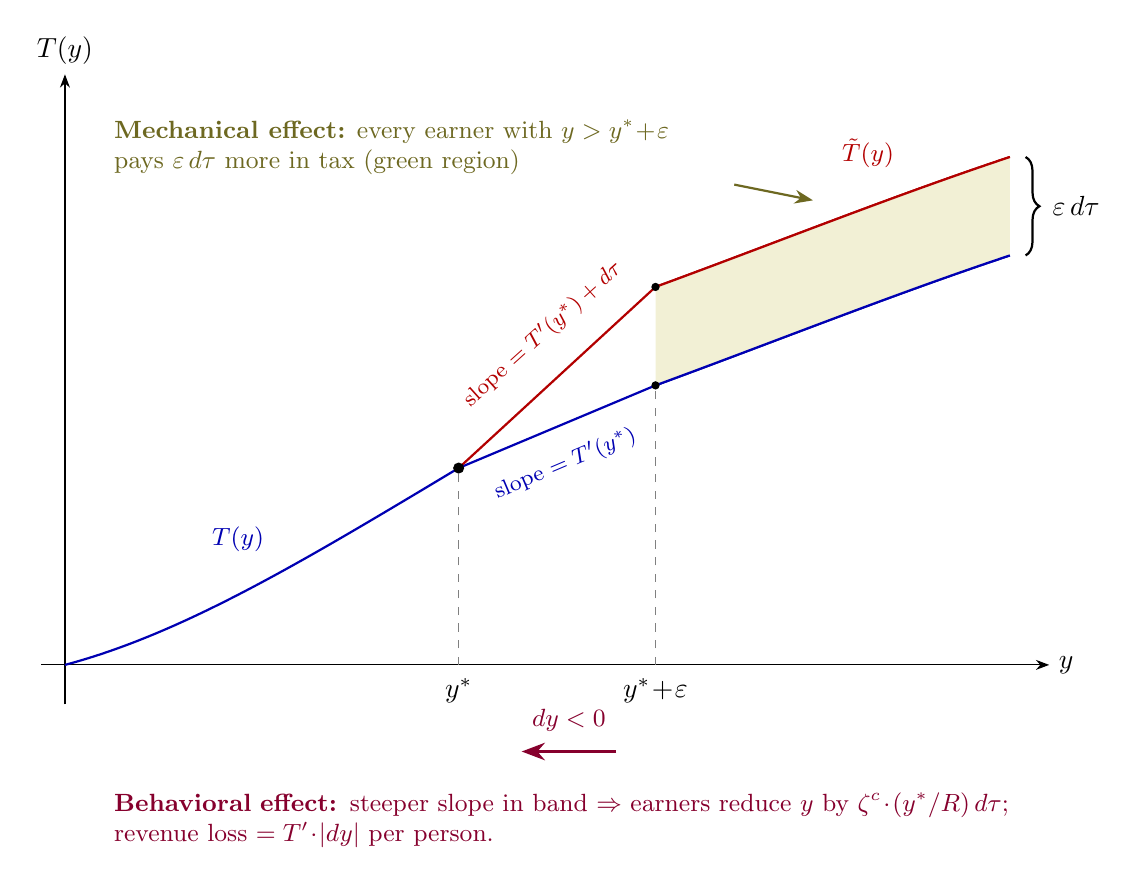
\begin{tikzpicture}[>=Stealth, x=1cm, y=1cm]

% --- Axes ---
\draw[->] (-0.3,0) -- (12.5,0) node[right] {$y$};
\draw[->] (0,-0.5) -- (0,7.5) node[above] {$T(y)$};

% ============================================================
% Baseline T(y): smooth increasing curve, origin to (12,5.2)
% ============================================================
% Segment 1: origin to y* (at x=5, T=2.5)
\draw[thick, blue!70!black]
  (0,0) .. controls (1.5,0.4) and (3,1.3) ..
  (5,2.5);

% Segment 2: baseline through band y* to y*+eps (x=5 to x=7.5)
% slope ~ 0.42
\draw[thick, blue!70!black]
  (5,2.5) -- (7.5,3.55);

% Segment 3: baseline above band (x=7.5 to x=12)
\draw[thick, blue!70!black]
  (7.5,3.55) .. controls (9,4.1) and (10.5,4.7) ..
  (12,5.2);

% ============================================================
% Perturbed T~(y): same until y*, steeper in band, shifted above
% ============================================================
% eps*dtau = 2.5 * 0.5 = 1.25 (exaggerated for visibility)

% In-band: steeper slope (baseline slope + dtau)
\draw[thick, red!70!black]
  (5,2.5) -- (7.5,4.8);

% Above band: parallel to baseline, shifted up by eps*dtau=1.25
\draw[thick, red!70!black]
  (7.5,4.8) .. controls (9,5.35) and (10.5,5.95) ..
  (12,6.45);

% Dashed: continue baseline above band for comparison
\draw[dashed, blue!50, thin]
  (7.5,3.55) .. controls (9,4.1) and (10.5,4.7) ..
  (12,5.2);

% ============================================================
% Vertical dashed lines at y* and y*+eps
% ============================================================
\draw[dashed, gray] (5,0) -- (5,2.5);
\draw[dashed, gray] (7.5,0) -- (7.5,3.55);
\node[below] at (5,-0.05) {$y^*$};
\node[below] at (7.5,-0.05) {$y^*\!+\!\varepsilon$};

% ============================================================
% Shading: gap between perturbed and baseline above band
% ============================================================
\fill[olive!12]
  % upper boundary (perturbed)
  (7.5,4.8)
  .. controls (9,5.35) and (10.5,5.95) ..
  (12,6.45)
  % right edge down
  -- (12,5.2)
  % lower boundary (baseline, reversed)
  .. controls (10.5,4.7) and (9,4.1) ..
  (7.5,3.55)
  -- cycle;

% Re-draw curves on top of shading
\draw[thick, blue!70!black]
  (7.5,3.55) .. controls (9,4.1) and (10.5,4.7) ..
  (12,5.2);
\draw[thick, red!70!black]
  (7.5,4.8) .. controls (9,5.35) and (10.5,5.95) ..
  (12,6.45);

% ============================================================
% eps*dtau brace on right edge
% ============================================================
\draw[decorate, decoration={brace, amplitude=5pt, mirror},
      thick] (12.2,5.2) -- (12.2,6.45)
  node[midway, right=6pt] {$\varepsilon\,d\tau$};

% ============================================================
% Slope annotations in the band
% ============================================================
% Baseline slope label (below the baseline segment in band)
\node[blue!70!black, font=\footnotesize, anchor=north,
      rotate=23]
  at (6.25,2.8) {slope $= T'(y^*)$};

% Perturbed slope label (above the perturbed segment in band)
\node[red!70!black, font=\footnotesize, anchor=south,
      rotate=42]
  at (6.25,4.0) {slope $= T'(y^*)+d\tau$};

% ============================================================
% Curve labels (well away from annotations)
% ============================================================
\node[blue!70!black, font=\small] at (2.2,1.6) {$T(y)$};
\node[red!70!black, font=\small] at (10.2,6.5) {$\tilde T(y)$};

% ============================================================
% Mechanical effect annotation (upper left, pointing to shading)
% ============================================================
\node[olive!70!black, align=left, font=\small,
      anchor=south west]
  at (0.5,6.5) {\textbf{Mechanical effect:} every earner
  with $y>y^*\!+\!\varepsilon$};
\node[olive!70!black, align=left, font=\small,
      anchor=south west]
  at (0.5,6.1) {pays $\varepsilon\,d\tau$ more in tax
  (green region)};
\draw[thick, olive!70!black, ->]
  (8.5,6.1) -- (9.5,5.9);

% ============================================================
% Behavioral effect annotation (bottom, well below curves)
% ============================================================
% Arrow showing income reduction
\draw[very thick, purple!70!black, ->]
  (7.0,-1.1) -- (5.8,-1.1);
\node[purple!70!black, font=\small] at (6.4,-0.7)
  {$dy<0$};

\node[purple!70!black, align=left, font=\small,
      anchor=north west, text width=11.5cm]
  at (0.5,-1.5)
  {\textbf{Behavioral effect:} steeper slope in band
  $\Rightarrow$ earners reduce $y$ by
  $\zeta^c\!\cdot\!(y^*/R)\,d\tau$;
  revenue loss $= T'\!\cdot\!|dy|$ per person.};

% ============================================================
% Dot at y* junction
% ============================================================
\fill (5,2.5) circle (2pt);
\fill (7.5,3.55) circle (1.5pt);
\fill (7.5,4.8) circle (1.5pt);

\end{tikzpicture}
\caption{The Saez perturbation.
The baseline schedule $T(y)$ (blue) is perturbed to
$\tilde T(y)$ (red) by increasing the slope by $d\tau$
in $[y^*,y^*+\varepsilon]$.
The two schedules coincide below $y^*$, diverge in the band
(where $\tilde T$ has a steeper slope), and run parallel
above it with a constant gap of $\varepsilon\,d\tau$.
At the optimum the mechanical gain and behavioral loss
exactly offset: $dM+dB=0$.}
\label{fig:saez-perturbation}
\end{figure}
\bigskip

\subsection{Deriving $dM$ and $dB$ from the Lagrangian}
\label{sec:mech}

We derive the effect of the perturbation on the planner's
Lagrangian. Recall from Section~\ref{sec:mechanism}:
\[
\mathcal{L}(T)
=
\int_{\zlow}^{\zbar} \psi(z)\,\calU(z)\,f(z)\,dz
\;+\;
\mu
\left[
\int_{\zlow}^{\zbar}
T(y(z))\,f(z)\,dz
\;-\; R_{\mathrm{gov}}
\right],
\]
where $\mu$ is the multiplier on the government budget
constraint (the marginal value of public funds, derived
in~\eqref{eq:mu_general}).

Write the perturbed schedule as
$\tilde T(y) = T(y) + \epsilon\,\delta T(y)$, where
\[
\delta T(y)
=
\begin{cases}
0, & y < y^*,\\
(y-y^*)\,d\tau, & y\in[y^*,y^*+\varepsilon],\\
\varepsilon\,d\tau, & y > y^*+\varepsilon,
\end{cases}
\]
and $\epsilon>0$ is a perturbation parameter (set to $1$ at the
end). Under the perturbed schedule, each agent's earnings adjust
from $y(z)$ to $y(z;\tilde T)$. The total derivative of the
Lagrangian at $\epsilon=0$ is
\begin{equation}
\label{eq:dL-total-1D}
\frac{d\mathcal L}{d\epsilon}\bigg|_{\epsilon=0}
=
\int_{\zlow}^{\zbar}
\biggl[
\underbrace{
  \psi(z)\frac{d\calU}{d\epsilon}
  + \mu\,\delta T(y)
}_{\text{(a)}}
\;+\;
\underbrace{
  \mu\,T'(y)\frac{\partial y}{\partial\epsilon}
}_{\text{(b)}}
\biggr]
f(z)\,dz.
\end{equation}
The revenue change
$d[T(y)]/d\epsilon = \delta T(y) + T'(y)\,\partial y/\partial\epsilon$
has been split into direct (in (a)) and behavioral (in (b))
components.

\begin{remark}[Connection to the Gâteaux derivative]
\label{rem:gateaux}
Expression \eqref{eq:dL-total-1D} is the \emph{Gâteaux derivative} of the planner's Lagrangian $\mathcal{L}$ at the tax schedule $T$ in the direction $\delta T$. Formally, $\mathcal{L}$ is a functional on the space of tax schedules, and
\[
  \frac{d\mathcal{L}}{d\epsilon}\bigg|_{\epsilon=0}
  = \lim_{\epsilon \to 0} \frac{\mathcal{L}(T + \epsilon\,\delta T) - \mathcal{L}(T)}{\epsilon}
  \equiv D\mathcal{L}(T;\, \delta T),
\]
which is the infinite-dimensional analogue of a directional derivative. At the optimum, $D\mathcal{L}(T;\, \delta T) = 0$ for all admissible directions $\delta T$---this is the necessary condition for optimality in function space. The Saez perturbation chooses a specific direction (a marginal rate increase in a narrow band), but the optimality condition must hold for \emph{every} such direction, which is what pins down the tax schedule pointwise. See Appendix~\ref{app:hamiltonian_primer} for the general variational framework.
\end{remark}

\paragraph{Envelope theorem and term (a).}
Each agent was already optimizing under $T$: the household FOC
$U_c(1-T'(y)) + U_n/z = 0$ holds at the current bundle. When the
schedule is perturbed, the agent re-optimizes (changing $y$),
but by the \textbf{envelope theorem} the welfare effect of
this behavioral adjustment is \emph{exactly zero}, not merely
second order. To see this, write the total change in
$\calU = U(y-T(y),\,y/z)$:
\[
\frac{d\calU}{d\epsilon}
= U_c\!\left[-\delta T(y)
  + \bigl(1-T'(y)\bigr)\frac{\partial y}{\partial\epsilon}
  \right]
+ \frac{U_n}{z}\frac{\partial y}{\partial\epsilon}.
\]
The terms involving $\partial y/\partial\epsilon$ cancel by the
household FOC ($U_c(1-T') + U_n/z = 0$), leaving
\[
\frac{d\calU}{d\epsilon}\bigg|_{\epsilon=0}
= -U_c\,\delta T(y).
\]
Thus the only welfare change comes from the direct tax increase
$\delta T(y)$, which reduces consumption dollar-for-dollar.
The behavioral adjustment \emph{does} matter for revenue
(term~(b)), because the government's revenue $T(y)$ depends on
the agent's choice---but it is the agent, not the government,
who was at an optimum. Therefore
\[
\psi(z)\frac{d\calU}{d\epsilon}
= -\psi(z)\,U_c\,\delta T(y).
\]
Defining the \textbf{marginal social welfare weight}
\begin{equation}
\label{eq:g-pert}
  g(z) := \frac{\psi(z)\,U_c(z)}{\mu},
\end{equation}
(so that $g(z)$ measures the social value---in dollars of
public funds---of one additional dollar to a type-$z$ agent),
term~(a) becomes
\begin{equation}
\label{eq:term-a-1D}
\text{(a)}
= \mu\,\delta T(y)\bigl(1 - g(z)\bigr).
\end{equation}
This is the \textbf{mechanical effect}: the net gain (revenue
minus welfare cost) from the direct tax increase, with behavior
held fixed.

\paragraph{Term (b): the behavioral revenue effect.}
The behavioral adjustment $\partial y/\partial\epsilon$ changes
government revenue by $T'(y)\,\partial y/\partial\epsilon$
per agent. (The agent's welfare effect from re-optimization
was already accounted for by the envelope theorem---it is zero.)
\begin{equation}
\label{eq:term-b-1D}
\text{(b)} = \mu\,T'(y)\frac{\partial y}{\partial\epsilon}.
\end{equation}
This is the \textbf{behavioral effect}: the revenue change
because agents adjust their earnings in response to the new
marginal incentives.

\paragraph{Slutsky decomposition of the behavioral effect.}
The behavioral response $\partial y/\partial\epsilon$ in
term~(b) includes both substitution and income effects:
\[
\frac{\partial y}{\partial\epsilon}
=
\underbrace{\frac{\partial y^c}{\partial\epsilon}}_{\text{substitution}}
+
\underbrace{\frac{\partial y^{\text{inc}}}{\partial\epsilon}}_{\text{income effect}}.
\]
We now compute the income-effect contribution to revenue
explicitly and show it can be absorbed into term~(a), leaving
only the compensated response in term~(b).

\paragraph{Step 1: The income-effect revenue.}
Define the \textbf{income effect on earnings}:
\[
  \eta(z) := -(1-T')\,\frac{\partial y}{\partial I} > 0,
\]
where $I$ is nonlabor income. Three ingredients enter this definition:
\begin{itemize}[leftmargin=2em]
  \item $\partial y/\partial I < 0$: the raw income effect---how earnings change when nonlabor income rises by \$1. Under normality of leisure, richer agents work less.
  \item The minus sign: a sign convention so that $\eta > 0$ under normality, measuring how much earnings \emph{fall} per unit increase in nonlabor income.
  \item The $(1-T')$ factor: normalizes the income effect per dollar of \emph{net-of-tax} income rather than gross income. This ensures the Slutsky relation in earnings space takes the clean form $\zeta^c = \zeta^u + \eta$, without awkward $1/(1-T')$ factors.
\end{itemize} The perturbation extracts
$\delta T(y) = \varepsilon\,d\tau$ from each earner above
$y^*$, which is equivalent to reducing nonlabor income by
$\delta T(y)$. The income-effect behavioral response in
earnings is therefore
\[
  dy_{\text{inc}}
  = \frac{\partial y}{\partial I}\cdot\delta T(y)
  = -\frac{\eta}{1-T'}\cdot\delta T(y).
\]
The revenue consequence of this earnings change is
$T'(y)\cdot dy_{\text{inc}}$, giving
\[
  \text{income-effect revenue per agent}
  = -\mu\,T'\cdot\frac{\eta}{1-T'}\cdot\delta T(y)
  = -\mu\,\frac{T'}{1-T'}\,\eta\cdot\delta T(y).
\]
The sign is positive (a revenue \emph{bonus}): the agent is
poorer, works more under normality, and pays more tax.

\paragraph{Step 2: Absorbing into term~(a).}
Combine the original mechanical effect (a) $= \mu\,\delta T(y)(1-g(z))$
with the income-effect revenue:
\begin{align*}
  \text{(a)} + \text{income-effect part of (b)}
  &= \mu\,\delta T(y)\!\left[(1-g(z)) + \frac{T'}{1-T'}\,\eta(z)\right] \\
  &= \mu\,\delta T(y)\!\left[1 - \underbrace{\left(g(z) - \frac{T'}{1-T'}\,\eta(z)\right)}_{\displaystyle =:\;\hat g(z)}\right].
\end{align*}
This motivates defining the \textbf{adjusted welfare weight}
\begin{equation}
\label{eq:ghat-pert}
  \hat g(z) := g(z) - \frac{T'(y(z))}{1-T'(y(z))}\,\eta(z).
\end{equation}
The adjustment $\frac{T'}{1-T'}\eta$ has two pieces:
$1/(1-T')$ de-normalizes $\eta$ (recovering the raw
$|\partial y/\partial I|$), and $T'$ converts the earnings
change into a revenue change. The adjusted weight $\hat g(z)$
is the net social cost of extracting a dollar from type $z$,
\emph{after crediting back} the income-effect revenue bonus.

\paragraph{Step 3: The redefined $dM$ and $dB$.}
We can now write the total effect of the perturbation as:
\begin{align}
dM &:= \text{(a) + income-effect part of (b)}
= \mu\,\delta T(y)\bigl(1-\hat g(z)\bigr),
\label{eq:dM-lagrangian-1D}
\\
dB &:= \text{compensated part of (b)}
= \mu\,T'(y)\frac{\partial y^c}{\partial\epsilon}.
\label{eq:dB-lagrangian-1D}
\end{align}
By construction, the two formulations are equivalent:
\[
\underbrace{(1-g)\,\delta T + T'\,\frac{\partial y}{\partial\epsilon}}_{\text{using }g\text{ and full }\partial y/\partial\epsilon}
\;=\;
\underbrace{(1-\hat g)\,\delta T + T'\,\frac{\partial y^c}{\partial\epsilon}}_{\text{using }\hat g\text{ and compensated }\partial y^c/\partial\epsilon},
\]
since the $\frac{T'}{1-T'}\eta$ subtracted from $g$ to
form $\hat g$ exactly equals the income-effect revenue moved
from~(b) into~(a). The Saez convention uses the second form
because the compensated elasticity $\zeta^c$ is the cleaner
behavioral primitive. Under quasilinear preferences
($U(c,n)=c-v(n)$), income effects vanish ($\eta=0$), so
$\hat g = g$ and the distinction disappears.

\subsection{Evaluating the mechanical effect $dM$}

Aggregating~\eqref{eq:dM-lagrangian-1D} over all agents
(dividing by $\mu$ to work in units of public funds) and
substituting $\delta T(y)$, the exact expression has three
pieces:
\begin{enumerate}[label=(\roman*)]
  \item Earners above the band ($y > y^*+\varepsilon$) each pay
    the full $\varepsilon\,d\tau$, contributing
    \[
      \varepsilon\,d\tau
      \int_{y^*+\varepsilon}^{\infty}
      \bigl(1-\hat g(y)\bigr)\,h(y)\,dy.
    \]
  \item Earners inside the band ($y\in[y^*,y^*+\varepsilon]$) pay
    only $(y-y^*)\,d\tau$, contributing
    \[
      d\tau\int_{y^*}^{y^*+\varepsilon}
      (y-y^*)\bigl(1-\hat g(y)\bigr)\,h(y)\,dy
      \;\le\;
      \varepsilon\,d\tau\cdot\varepsilon\,
      \sup|{(1-\hat g)\,h}|
      = O(\varepsilon^2\,d\tau).
    \]
  \item Replacing the lower limit $y^*+\varepsilon$ by $y^*$ in
    (i) changes the integral by
    $\int_{y^*}^{y^*+\varepsilon}(1-\hat g)\,h\,dy = O(\varepsilon)$,
    so the error is $\varepsilon\,d\tau\cdot O(\varepsilon)
    = O(\varepsilon^2\,d\tau)$.
\end{enumerate}
Combining (i)--(iii), the mechanical effect is
\begin{equation}
\label{eq:dM-pert}
  dM = \varepsilon\,d\tau
  \int_{y^*}^{\infty}
  \bigl(1-\hat g(y)\bigr)\,h(y)\,dy
  + O(\varepsilon^2\,d\tau),
\end{equation}
where $\hat g(y) \equiv \hat g(z(y))$.
The $O(\varepsilon^2)$ remainder is negligible: the first-order
condition divides by $\varepsilon\,d\tau$ and sends
$\varepsilon\to 0$.

\begin{remark}[Budget-balance normalization]
\label{rem:budget_balance}
The adjusted welfare weights integrate to one: $\int_0^\infty \hat g(y)\,h(y)\,dy = 1$. To see this, consider a uniform lump-sum tax $\delta T(y) = \varepsilon\,d\tau$ on \emph{all} earners (i.e., set $y^* = 0$). The mechanical effect is
\[
  dM = \varepsilon\,d\tau \int_{0}^{\infty} (1 - \hat g(y))\,h(y)\,dy.
\]
At the optimum, this reform must generate zero first-order welfare change (the planner has already optimized the lump-sum component of the tax). Since $\varepsilon\,d\tau > 0$, we need $\int (1 - \hat g)\,h\,dy = 0$, i.e., $\int \hat g\,h\,dy = 1$. Intuitively, a uniform lump-sum transfer is a pure redistribution of the numeraire; the total social value of a dollar distributed to everyone must equal the social cost of collecting it ($\mu$), which is normalized to one.
\end{remark}

\subsection{Evaluating the behavioral effect $dB$}
\label{sec:behav}

As shown in~\eqref{eq:dB-lagrangian-1D}, the behavioral effect
captures only the compensated earnings response.
An agent of type $z$ at income $y^*$ faces a marginal rate
increase of $d\tau$ in the band, changing the local
net-of-tax rate from $R(y^*) = 1-T'(y^*)$ to
$R(y^*)-d\tau$, i.e.\ $d(1-\tau) = -d\tau$.

To compute the compensated response $dy^c$, we use the ETI
from~\eqref{eq:ETI-def}, which is defined via the linearized
schedule
$T^{\mathrm{lin}}$~\eqref{eq:linearized-schedule-pert}. This applies
to the nonlinear perturbation because the virtual linearization at
$y^*$ satisfies $T^{\mathrm{lin}}(y^*) = T(y^*)$ and
$T^{\mathrm{lin}\prime}(y^*) = T'(y^*)$ by construction---the budget
constraint under $T^{\mathrm{lin}}$ is \emph{tangent} to the one
under $T$ at the current optimum. The first-order response to a
marginal rate change depends only on the slope and level of the
budget constraint, not on the curvature $T''$ (which enters only
at second order), so the first-order compensated responses under
$T$ and $T^{\mathrm{lin}}$ coincide.

Rearranging the ETI definition:
\[
  \zeta^c(y)
  = \frac{\partial \hat{y}^{\,c}}{\partial(1-\tau)}
  \cdot\frac{1-\tau}{y}
  \qquad\Longrightarrow\qquad
  \frac{\partial \hat{y}^{\,c}}{\partial(1-\tau)}
  = \zeta^c(y)\,\frac{y}{R(y)},
\]
and applying the chain rule with $d(1-\tau) = -d\tau$:
\[
  dy^c
  = \frac{\partial \hat{y}^{\,c}}{\partial(1-\tau)}\,d(1-\tau)
  = -\zeta^c(y^*)\,\frac{y^*}{R(y^*)}\,d\tau.
\]
The sign is negative: a higher marginal rate reduces the
net-of-tax rate, causing compensated earnings to fall.

The resulting revenue loss per affected agent at income $y$ is
$T'(y)\,|dy^c(y)|$, and the density of agents at $y$ is
$h(y)$. Only agents \emph{inside} the band $[y^*,y^*+\varepsilon]$ face a changed marginal rate; agents outside the band face no marginal incentive change (they experience only a lump-sum shift, which is already captured in $dM$ via $\hat g$).

Aggregating the compensated revenue loss over the band:
\[
  dB = \int_{y^*}^{y^*+\varepsilon} T'(y)\,dy^c(y)\,h(y)\,dy.
\]
Within the band, $dy^c(y)$ and $h(y)$ are continuous, so
$T'(y)\,dy^c(y)\,h(y) = T'(y^*)\,dy^c(y^*)\,h(y^*) + O(\varepsilon)$.
Since the band has width $\varepsilon$, the integral evaluates to
\[
  dB = \varepsilon \cdot T'(y^*)\,dy^c(y^*)\,h(y^*) + O(\varepsilon^2\,d\tau).
\]
Substituting $dy^c(y^*) = -\zeta^c(y^*)\,\frac{y^*}{R(y^*)}\,d\tau$ and $R(y^*) = 1 - T'(y^*)$:
\begin{equation}
\label{eq:dB-pert}
  dB = -\varepsilon\,d\tau\,
  \frac{T'(y^*)}{1-T'(y^*)}\,
  \zeta^c(y^*)\,y^*\,h(y^*)
  + O(\varepsilon^2\,d\tau).
\end{equation}
As with $dM$, the $O(\varepsilon^2\,d\tau)$ remainder vanishes after dividing by $\varepsilon\,d\tau$ and sending $\varepsilon \to 0$.

\subsection{First-order condition}

At the optimum, the total effect of the perturbation must be zero
for every $y^*$:
\[
  dM + dB = 0.
\]
Substituting~\eqref{eq:dM-pert} and~\eqref{eq:dB-pert}, cancelling
$\varepsilon\,d\tau>0$, and rearranging:
\begin{equation}
\label{eq:FOC-pert}
  \boxed{
  \frac{T'(y^*)}{1-T'(y^*)}
  = \frac{1}{\zeta^c(y^*)}
  \cdot \frac{1}{y^*\,h(y^*)}
  \int_{y^*}^{\infty}
  \bigl(1-\hat g(y)\bigr)\,h(y)\,dy.
  }
\end{equation}

This is the \emph{Saez (2001) optimal tax formula}. The
tax wedge $T'/(1-T')$ at income $y^*$ equals:
\begin{itemize}
  \item $1/\zeta^c(y^*)$: the inverse compensated ETI
    (higher elasticity $\Rightarrow$ lower tax),
  \item $\displaystyle\frac{1-H(y^*)}{y^*\,h(y^*)}$: the
    inverse hazard rate of the earnings distribution
    (thicker tail $\Rightarrow$ higher tax),
  \item $\displaystyle\frac{1}{1-H(y^*)}\int_{y^*}^{\infty}
    (1-\hat g(y))\,h(y)\,dy$: one minus the average adjusted
    welfare weight above $y^*$ (less concern for the rich
    $\Rightarrow$ higher tax).
\end{itemize}

\subsection{Equivalence with the Hamiltonian formula}

Formula~\eqref{eq:FOC-pert} is equivalent to the Hamiltonian
formula~\eqref{eq:general_tax}. To see this, change variables
from $y$ to $z$ using $h(y)\,dy = f(z)\,dz$ and
$\zeta^c(y) = \varepsilon^c(z)$:
\[
  \frac{T'(y(z))}{1-T'(y(z))}
  = \frac{1}{\varepsilon^c(z)}
  \cdot \frac{1}{y(z)\,h(y(z))}
  \int_{z}^{\zbar}
  \bigl(1-\hat g(\zeta)\bigr)\,f(\zeta)\,d\zeta.
\]
Using $y(z)\,h(y(z)) = z\,n(z)\,f(z)/y'(z)$ and the
identity~\eqref{eq:key_ratio}, together with the integral
representation of the costate $\lambda(z)$
from~\eqref{eq:lambda_solution}, one recovers exactly the
three-factor structure of~\eqref{eq:general_tax}. The
perturbation approach makes the economic forces transparent,
while the Hamiltonian approach provides the mathematical
machinery for existence and uniqueness.

\subsection{Optimal top rate from the perturbation formula}
\label{sec:top-rate-pert}

The perturbation formula yields the Diamond--Saez top rate
directly. Take $y^*\to\infty$ and assume:
\begin{enumerate}[label=(\alph*)]
  \item Zero welfare weight in the tail:
    $\hat g(y)\to 0$ as $y\to\infty$.
  \item Pareto tail in earnings: $1-H(y)\propto y^{-\alpha_y}$,
    so that $\frac{1-H(y)}{y\,h(y)}\to\frac{1}{\alpha_y}$.
  \item Constant compensated ETI at the top:
    $\zeta^c(y)\to e$.
\end{enumerate}
Under these conditions, $(1-\hat g)\to 1$ in the numerator and
\eqref{eq:FOC-pert} reduces to
\[
  \frac{T'}{1-T'}
  = \frac{1}{e}\cdot\frac{1}{\alpha_y}
  = \frac{1}{\alpha_y\,e},
\]
giving
\[
  T'_{\text{top}} = \frac{1}{1+\alpha_y\,e},
\]
which matches~\eqref{eq:top_rate_DS}.

%==========================================================================
\section{Special Cases and the ABC Formula}
\label{sec:special}
%==========================================================================

\subsection{Separable preferences}

With $U(c,n) = u(c) - v(n)$, the non-separable term vanishes: $H_{U,N}(z) = 0$. The formulas simplify considerably.

\paragraph{Lagrange multiplier.}
\begin{equation}
\label{eq:mu_sep}
  \mu = \frac{\displaystyle\int_{\zlow}^{\zbar} \psi(\zeta) \, f(\zeta) \, d\zeta}
             {\displaystyle\int_{\zlow}^{\zbar} \bigl[u'(c(\zeta))\bigr]^{-1} \, f(\zeta) \, d\zeta}
  = \frac{1}{\displaystyle\int_{\zlow}^{\zbar} \bigl[u'(c(\zeta))\bigr]^{-1} \, f(\zeta) \, d\zeta},
\end{equation}

\paragraph{Costate.} Since $H_{U,N} = 0$, the exponential in \eqref{eq:lambda_solution} equals one:
\begin{equation}
\label{eq:lambda_sep}
  \lambda(z) = \int_{z}^{\zbar} \left[ \psi(\zeta) - \frac{\mu}{u'(c(\zeta))} \right] f(\zeta) \, d\zeta.
\end{equation}

\paragraph{Tax formula.} Define the \emph{marginal social welfare weight} of type $z$:
\begin{equation}
\label{eq:g_weight}
  g(z) = \frac{u'(c(z)) \, \psi(z)}{\mu}.
\end{equation}
This measures the social value (in units of public funds) of transferring one unit of resources to type $z$. Then
\begin{equation}
\label{eq:tax_sep}
  \frac{T'(y(z))}{1 - T'(y(z))}
  = \frac{1 + \varepsilon^u(z)}{\varepsilon^c(z)} \cdot \frac{u'(c(z))}{z \, f(z)}
    \int_{z}^{\zbar} \frac{1 - g(\zeta)}{u'(c(\zeta))} \, f(\zeta) \, d\zeta.
\end{equation}

\begin{proof}
Substituting \eqref{eq:lambda_sep} into \eqref{eq:general_tax} and using $U_c = u'(c)$:
\[
  \frac{T'}{1-T'} = -\frac{1+\varepsilon^u}{\varepsilon^c} \cdot \frac{u'(c(z))}{z \, f(z) \, \mu}
  \int_{z}^{\zbar} \left[ \psi(\zeta) - \frac{\mu}{u'(c(\zeta))} \right] f(\zeta) \, d\zeta.
\]
Distributing the minus sign and pulling $1/\mu$ inside:
\[
  = \frac{1+\varepsilon^u}{\varepsilon^c} \cdot \frac{u'(c(z))}{z \, f(z)}
  \int_{z}^{\zbar} \frac{1}{u'(c(\zeta))} \left[ 1 - \frac{\psi(\zeta) \, u'(c(\zeta))}{\mu} \right] f(\zeta) \, d\zeta.
\]
Recognizing the definition of $g$ completes the derivation.
\end{proof}

\subsection{The Diamond (1998) ABC formula}

Following Diamond (1998), assume quasilinear-in-consumption preferences $U(c,n) = c - v(n)$. Define the ``welfare cdf''
\[
  \Psi(z) = \int_{\zlow}^{z} \psi(\zeta) \, f(\zeta) \, d\zeta.
\]
Since $u'(c) = 1$, we have $\mu = 1$ and $g(z) = \psi(z)$. For redistributive preferences, $\psi(z)$ is decreasing in $z$. The tax formula \eqref{eq:tax_sep} becomes
\[
  \frac{T'(y(z))}{1 - T'(y(z))}
  = \frac{1+\varepsilon^u(z)}{\varepsilon^c(z)} \cdot \frac{1}{z \, f(z)}
  \int_{z}^{\zbar} \bigl[ 1 - \psi(\zeta) \bigr] f(\zeta) \, d\zeta.
\]
Evaluating the integral:
\[
  \int_{z}^{\zbar} f(\zeta) \, d\zeta - \int_{z}^{\zbar} \psi(\zeta) \, f(\zeta) \, d\zeta
  = \bigl[1 - F(z)\bigr] - \bigl[1 - \Psi(z)\bigr] = \Psi(z) - F(z).
\]
Hence
\begin{equation}
\label{eq:ABC_quasi}
  \frac{T'(y(z))}{1 - T'(y(z))} = \frac{1+\varepsilon^u(z)}{\varepsilon^c(z)} \cdot \frac{\Psi(z) - F(z)}{z \, f(z)}.
\end{equation}

For the more general separable case $U(c,n) = u(c) - v(n)$, define the inverse-marginal-utility weighted density and its cdf. Let
\[
  R \equiv \int_{\zlow}^{\zbar} \frac{f(\zeta)}{u'(c(\zeta))} \, d\zeta
\]
denote the total inverse-marginal-utility-weighted mass. Then define the weighted density and its cdf:
\[
  \omega(z) = \frac{f(z) / u'(c(z))}{R}, \qquad
  \Omega(z) = \int_{\zlow}^{z} \omega(\zeta) \, d\zeta.
\]
The tax formula generalizes to
\begin{equation}
\label{eq:ABC_separable}
  \frac{T'(y(z))}{1 - T'(y(z))} = \frac{1+\varepsilon^u(z)}{\varepsilon^c(z)} \cdot \frac{\Psi(z) - \Omega(z)}{z \, \omega(z)}.
\end{equation}
When $u(c) = c$, we recover $\Omega = F$, $\omega = f$, and \eqref{eq:ABC_quasi}.

\paragraph{The ABC decomposition.} Diamond (1998) decomposes this as
\begin{equation}
\label{eq:ABC}
  \frac{T'(y(z))}{1 - T'(y(z))} =
  \underbrace{\frac{1+\varepsilon^u(z)}{\varepsilon^c(z)}}_{A(z)}
  \;\cdot\;
  \underbrace{\frac{\Psi(z) - \Omega(z)}{1 - \Omega(z)}}_{B(z)}
  \;\cdot\;
  \underbrace{\frac{1 - \Omega(z)}{z \, \omega(z)}}_{C(z)}.
\end{equation}
\begin{itemize}[leftmargin=2em]
  \item $A(z)$: \textbf{Elasticity effect.} Higher labor supply elasticity $\Rightarrow$ lower $A$ $\Rightarrow$ lower marginal tax. Captures the efficiency cost of distorting labor supply.

  \item $B(z)$: \textbf{Redistribution motive.} We can write $B(z) = 1 - \frac{1 - \Psi(z)}{1 - \Omega(z)}$. The numerator $1 - \Psi(z)$ is the planner's welfare weight on types above $z$; the denominator $1 - \Omega(z)$ is the (inverse-marginal-utility-weighted) mass above $z$. When the planner puts relatively less weight on the rich ($\Psi(z) > \Omega(z)$), we have $B(z) > 0$, calling for positive taxation. When the planner is indifferent to redistribution ($\Psi = \Omega$), $B(z) = 0$ and all taxes vanish.

  \item $C(z)$: \textbf{Tail shape.} The ratio $(1 - \Omega(z))/(z \, \omega(z))$ is the (weighted) inverse hazard rate of the type distribution. A thicker tail (more mass above $z$ relative to density at $z$) raises $C$ and calls for higher taxes, because many agents in the tail contribute revenue while only those at $z$ are directly distorted.
\end{itemize}

\subsection{Optimal top marginal tax rate}

Consider the upper tail of the type distribution. Assume:
\begin{enumerate}[label=(\alph*)]
  \item Quasilinear-in-consumption preferences: $U(c,n) = c - \psi \frac{n^{1+\gamma}}{1+\gamma}$, so $\varepsilon^f = \varepsilon^u = \varepsilon^c = 1/\gamma$.
  \item No welfare weight on the tail: $\Psi(z) = 1$ for large $z$.
  \item The type distribution has a Pareto tail with shape parameter $\alpha$: $1 - F(z) \propto z^{-\alpha}$ for large $z$, implying $\frac{1-F(z)}{z \, f(z)} = \frac{1}{\alpha}$.
\end{enumerate}

Under these assumptions, the tax formula \eqref{eq:ABC_quasi} becomes
\[
  \frac{T'}{1-T'} = (1 + \gamma) \cdot \frac{1 - F(z)}{z \, f(z)} = \frac{1+\gamma}{\alpha}.
\]
Solving:
\begin{equation}
\label{eq:top_rate_z}
  T' = \frac{1}{1 + \dfrac{\alpha}{1+\gamma}}.
\end{equation}

\paragraph{Rewriting in terms of the earnings distribution.} Since the optimal labor supply satisfies $\psi n^\gamma = (1-T')z$, with a constant marginal tax rate $\nu = 1-T'$ in the tail we have
\[
  y(z) = zn(z) = z \left(\frac{\nu z}{\psi}\right)^{1/\gamma}
  = \left(\frac{\nu}{\psi}\right)^{1/\gamma} z^{(1+\gamma)/\gamma}.
\]
If $z$ is Pareto with shape $\alpha$, then earnings $y$ are Pareto with shape
\[
  \alpha_y = \frac{\alpha \gamma}{1+\gamma}
  \qquad \Longleftrightarrow \qquad
  \alpha = \frac{1+\gamma}{\gamma}\,\alpha_y.
\]

\begin{proof}
For $\bar y$ in the tail:
\begin{align*}
  \Pr(y > \bar y) &= \Pr\!\left(z > \bar y^{\,\gamma/(1+\gamma)} \left(\frac{\psi}{\nu}\right)^{1/(1+\gamma)}\right)
  \propto \left(\bar y^{\,\gamma/(1+\gamma)}\right)^{-\alpha} = \bar y^{\,-\alpha\gamma/(1+\gamma)}.
\end{align*}
Hence $y$ is Pareto with shape $\alpha_y = \alpha\gamma/(1+\gamma)$.
\end{proof}

Let $e = 1/\gamma$ denote the earnings elasticity with respect to the net-of-tax rate. Then
\[
  \frac{\alpha}{1+\gamma} = \frac{\alpha_y}{\gamma} = \alpha_y \, e.
\]
Therefore, the top tax rate in terms of observables is
\begin{equation}
\label{eq:top_rate_DS}
  \boxed{
  T'_{\text{top}} = \frac{1}{1 + \alpha_y \, e},
  }
\end{equation}
which is the Diamond--Saez formula. With empirically plausible values---$\alpha_y \approx 1.5$ (Pareto coefficient of the U.S.\ earnings distribution) and $e \approx 0.25$ (compensated earnings elasticity)---this yields $T'_{\text{top}} \approx 1/(1 + 0.375) \approx 73\%$.

\subsection{Zero tax at the bottom}

At the bottom of the distribution $z = \zlow$, the boundary condition $\lambda(\zlow) = 0$ combined with the tax formula \eqref{eq:general_tax} immediately implies
\[
  T'(y(\zlow)) = 0.
\]
Intuitively, a marginal tax on the lowest type distorts that type's labor supply but generates no redistributive benefit (there is no one below to redistribute to).

\begin{remark}[Sensitivity of bottom tax rates]
The zero-at-the-bottom result depends critically on the assumption that the lower bound of the productivity distribution is strictly positive ($\zlow > 0$). If instead the support extends to zero ($\zlow = 0$), the optimal marginal tax rate at the bottom converges to 100\%, because the marginal disutility of producing the first dollar of income vanishes for any $z > 0$, making the indifference curve locally flat at zero income. In the baseline calibration with $\zlow > 0$, the zero-rate region is vanishingly small and marginal rates rise rapidly from the bottom.

More broadly, Heathcote and Tsujiyama (2026) show that optimal tax rates at low income levels are surprisingly sensitive to how one models zero-earning individuals. A mass of zero-productivity types (a ``disability'' interpretation) generates a U-shaped marginal tax profile with high rates over a wide range at the bottom. A fixed utility cost of labor force participation (a ``costly participation'' interpretation) instead delivers low, increasing rates at the bottom.  These findings highlight that the classic zero-at-the-bottom result, while theoretically correct for the standard model with $\zlow > 0$, offers limited practical guidance for designing transfers at the bottom of the income distribution.
\end{remark}

\subsection{Zero tax at the top (with bounded support)}

Similarly, at $z = \zbar$ with $\lambda(\zbar) = 0$:
\[
  T'(y(\zbar)) = 0.
\]
The reasoning is symmetric: a marginal tax increase on the highest type generates no revenue from types above (there are none), so it is purely distortionary. With an unbounded Pareto tail, this result does not apply and the limiting tax rate is given by \eqref{eq:top_rate_DS}.

\subsection{Summary of forces}

The optimal tax schedule balances three forces at every income level:
\begin{enumerate}[label=\arabic*., leftmargin=2em]
  \item \textbf{Equity:} Higher taxes enable redistribution from richer to poorer households. The redistribution motive is captured by $B(z)$ and the social welfare weights $g(z)$.

  \item \textbf{Efficiency:} Higher taxes distort labor supply. The efficiency cost is governed by the elasticities $\varepsilon^u$ and $\varepsilon^c$, summarized in $A(z)$.

  \item \textbf{Revenue:} The shape of the income distribution determines how many taxpayers are affected by the tax at each point. A thicker tail (lower hazard rate) means more revenue per unit of distortion, summarized in $C(z)$.
\end{enumerate}

%==========================================================================
\section{Computational Approaches}
\label{sec:computation}
%==========================================================================

Computing optimal tax schedules requires solving a challenging fixed-point problem: the tax schedule determines behavior, which in turn determines the optimal tax schedule. This section presents three computational approaches, following Heathcote and Tsujiyama (2026). Throughout, we work with the separable preference specification
\[
  u(c,y;z) = \log c - \frac{1}{1+\sigma}\left(\frac{y}{z}\right)^{1+\sigma},
\]
where $1/\sigma$ is the Frisch elasticity of labor supply. We discretize the productivity distribution onto a grid $\{z_1, \ldots, z_N\}$ with probabilities $\{\pi_1, \ldots, \pi_N\}$, evenly spaced in logs. The \emph{coarseness} of the grid is $\kappa = z_{i+1}/z_i = (z_N/z_1)^{1/(N-1)}$.

\subsection{Mirrlees approach}
\label{sec:mirrlees_approach}

The \emph{Mirrlees approach} directly solves for the constrained-efficient allocation by choosing type-specific consumption and income bundles. With our preference class, the local incentive compatibility constraints are necessary and sufficient for global IC. These consist of downward incentive constraints (DIC) and upward incentive constraints (UIC):
\begin{align}
  U(z_i, z_i) &\geq U(z_i, z_{i-1}), \quad i = 2, \ldots, N, \tag{DIC} \label{eq:DIC} \\
  U(z_{i-1}, z_{i-1}) &\geq U(z_{i-1}, z_i), \quad i = 2, \ldots, N. \tag{UIC} \label{eq:UIC}
\end{align}
We now argue that, at the optimum, the DICs are binding and the UICs reduce to a monotonicity condition.

\paragraph{DICs are binding.}
Suppose for contradiction that the DIC for type $i$ is slack:
\[
  \log(c_i) - \frac{(y_i/z_i)^{1+\sigma}}{1+\sigma} > \log(c_{i-1}) - \frac{(y_{i-1}/z_i)^{1+\sigma}}{1+\sigma}.
\]
Then the planner can reduce $c_i$ by $\epsilon$ and increase $c_{i-1}$ by $\epsilon\,\pi_i/\pi_{i-1}$, keeping the resource constraint satisfied. The welfare change is
\[
  \pi_i\!\left(-\frac{1}{c_i}\right) + \pi_{i-1}\!\left(\frac{1}{c_{i-1}}\right)\frac{\pi_i}{\pi_{i-1}} = \pi_i\!\left(\frac{1}{c_{i-1}} - \frac{1}{c_i}\right) > 0,
\]
where the inequality holds because $c_{i-1} < c_i$ (lower types consume less at any IC allocation). It remains to verify that, for small $\epsilon$, no IC constraint is violated by this perturbation:
\begin{itemize}[leftmargin=2em]
  \item \textbf{DIC for type $i$} (the slack one): Both $\log(c_i)$ decreases and $\log(c_{i-1})$ increases, tightening the constraint from both sides. But since it was strictly slack, continuity guarantees it remains satisfied for small enough $\epsilon$.
  \item \textbf{DIC for type $i+1$}: This requires $\calU_{i+1} \geq U(z_{i+1}, z_i)$, and the RHS involves $\log(c_i)$, which decreases. The constraint is \emph{relaxed}.
  \item \textbf{DIC for type $i-1$} (if $i \geq 3$): This requires $\calU_{i-1} \geq U(z_{i-1}, z_{i-2})$, and the LHS involves $\log(c_{i-1})$, which increases. The constraint is \emph{relaxed}.
  \item \textbf{UIC for type $i-1$}: This requires $\calU_{i-1} \geq U(z_{i-1}, z_i)$. The LHS increases (higher $c_{i-1}$) and the RHS decreases (lower $c_i$), so the constraint is \emph{relaxed}.
  \item \textbf{UIC for type $i$}: This requires $\calU_i \geq U(z_i, z_{i+1})$. The LHS decreases (lower $c_i$), tightening the constraint. But the UIC was satisfied (by monotonicity), so it remains satisfied for small $\epsilon$.
\end{itemize}
All other constraints are unaffected (only $c_i$ and $c_{i-1}$ change). Thus the perturbation is feasible and welfare-improving, contradicting optimality.

\paragraph{UICs hold if and only if $y_i \geq y_{i-1}$.}
This is the discrete single-crossing argument. With every DIC binding, type $i+1$ is \emph{indifferent} between its own bundle $(c_{i+1}, y_{i+1})$ and type $i$'s bundle $(c_i, y_i)$:
\[
  \log(c_{i+1}) - \frac{(y_{i+1}/z_{i+1})^{1+\sigma}}{1+\sigma} = \log(c_i) - \frac{(y_i/z_{i+1})^{1+\sigma}}{1+\sigma}.
\]
The UIC for type $i$ requires that $i$ weakly prefers its own bundle to $i+1$'s:
\[
  \log(c_i) - \frac{(y_i/z_i)^{1+\sigma}}{1+\sigma} \geq \log(c_{i+1}) - \frac{(y_{i+1}/z_i)^{1+\sigma}}{1+\sigma}.
\]
Subtracting the binding DIC from the UIC and rearranging:
\[
  \frac{y_{i+1}^{1+\sigma}}{1+\sigma}\!\left(\frac{1}{z_i^{1+\sigma}} - \frac{1}{z_{i+1}^{1+\sigma}}\right) \geq \frac{y_i^{1+\sigma}}{1+\sigma}\!\left(\frac{1}{z_i^{1+\sigma}} - \frac{1}{z_{i+1}^{1+\sigma}}\right).
\]
Since $z_i < z_{i+1}$, the factor $1/z_i^{1+\sigma} - 1/z_{i+1}^{1+\sigma} > 0$, and dividing through gives $y_{i+1}^{1+\sigma} \geq y_i^{1+\sigma}$, i.e., $y_{i+1} \geq y_i$.

We now show the converse direction holds as well, establishing the full equivalence. Suppose $y_{i+1} \geq y_i$. We must show the UIC for type $i$ holds: $U(c_i, y_i/z_i) \geq U(c_{i+1}, y_{i+1}/z_i)$, i.e.,
\[
  \log(c_i) - \frac{(y_i/z_i)^{1+\sigma}}{1+\sigma} \geq \log(c_{i+1}) - \frac{(y_{i+1}/z_i)^{1+\sigma}}{1+\sigma}.
\]
From the binding DIC for type $i+1$:
\[
  \log(c_{i+1}) - \log(c_i) = \frac{(y_{i+1}/z_{i+1})^{1+\sigma} - (y_i/z_{i+1})^{1+\sigma}}{1+\sigma}.
\]
Substituting into the UIC requirement and rearranging:
\[
  \frac{y_{i+1}^{1+\sigma} - y_i^{1+\sigma}}{1+\sigma} \cdot \frac{1}{z_i^{1+\sigma}}
  \geq \frac{y_{i+1}^{1+\sigma} - y_i^{1+\sigma}}{1+\sigma} \cdot \frac{1}{z_{i+1}^{1+\sigma}}.
\]
Since $y_{i+1} \geq y_i$, the factor $y_{i+1}^{1+\sigma} - y_i^{1+\sigma} \geq 0$. Since $z_i < z_{i+1}$, we have $1/z_i^{1+\sigma} > 1/z_{i+1}^{1+\sigma}$. The product of a nonneg\-ative and a positive factor is nonneg\-ative, so the inequality holds. (It is strict whenever $y_{i+1} > y_i$.)

Conversely, if $y_{i+1} < y_i$, the factor $y_{i+1}^{1+\sigma} - y_i^{1+\sigma} < 0$ reverses the inequality, violating the UIC.

\begin{remark}[Connection to single crossing]
The algebraic argument above is the discrete incarnation of the continuous single-crossing proof in Appendix~\ref{app:SC_proof}. The factor $1/z_i^{1+\sigma} - 1/z_{i+1}^{1+\sigma} > 0$ is the discrete analogue of the slope difference $S(c,y,z_i) - S(c,y,z_{i+1}) > 0$ (Lemma~\ref{lem:SC_slopes}): producing a given output costs more labor disutility for the less productive type. The monotonicity condition $y_{i+1} \geq y_i$ ensures that the allocation does not ask the less productive type to produce more, which would create an incentive to swap bundles.
\end{remark}

\medskip

The planner's problem is therefore:
\begin{align}
  &\max_{\{c_i, y_i\}_{i=1}^{N}} \;\; \sum_{i=1}^{N} \pi_i \left[\log(c_i) - \frac{1}{1+\sigma}\left(\frac{y_i}{z_i}\right)^{1+\sigma}\right] \label{eq:mirrlees_obj} \\
  &\text{s.t.} \quad \log(c_i) - \frac{(y_i/z_i)^{1+\sigma}}{1+\sigma} = \log(c_{i-1}) - \frac{(y_{i-1}/z_i)^{1+\sigma}}{1+\sigma}, \quad i = 2, \ldots, N, \label{eq:DIC_explicit} \\
  &\phantom{\text{s.t.}} \quad y_i \geq y_{i-1}, \quad i = 2, \ldots, N, \label{eq:monotone} \\
  &\phantom{\text{s.t.}} \quad \sum_{i=1}^{N} \pi_i y_i \geq \sum_{i=1}^{N} \pi_i c_i + G. \label{eq:RC_discrete}
\end{align}

Denoting by $\delta_i$ the multiplier on the DIC for type $i$ and by $\mu$ the multiplier on the resource constraint, the first-order conditions with respect to $c_i$ and $y_i$ are:
\begin{align}
  c_i^{-1}(\pi_i + \delta_i - \delta_{i+1}) &= \mu \pi_i, \label{eq:FOC_c} \\
  \frac{y_i^{\sigma}}{z_i^{1+\sigma}}(\pi_i + \delta_i) - \frac{y_i^{\sigma}}{z_{i+1}^{1+\sigma}}\delta_{i+1} &= -\mu\pi_i, \label{eq:FOC_y}
\end{align}
with $\delta_1 = 0$ and $\delta_{N+1} = 0$.  Rather than solving these FOCs directly, we exploit the binding-DIC structure to eliminate~$c$ and solve an unconstrained problem in~$y$ (see below).

Given the optimal allocation $\{y_i^*, c_i^*\}$, the implied marginal tax rates follow from the household's first-order condition in the decentralized economy:
\begin{equation}
  T_i^{*\prime} = 1 - \frac{c_i^*}{z_i}\left(\frac{y_i^*}{z_i}\right)^{\sigma}.
  \label{eq:mirrlees_mtr}
\end{equation}

\paragraph{Eliminating consumption via binding DIC.}
Because every DIC binds at the optimum, consumption is pinned by income alone (up to a single level $c_1$).  Writing $n_i = y_i/z_i$, the binding DIC for type~$i$ gives
\begin{equation}
  \log c_i = \log c_{i-1} + \underbrace{\frac{n_i^{1+\sigma} - (y_{i-1}/z_i)^{1+\sigma}}{1+\sigma}}_{S_i - S_{i-1}},
  \label{eq:DIC_chain}
\end{equation}
so $c_i = c_1 \exp(S_i)$ where $S_1 = 0$ and $S_i = \sum_{j=2}^{i}[n_j^{1+\sigma} - (y_{j-1}/z_j)^{1+\sigma}]/(1+\sigma)$.  The level~$c_1$ is then determined by the resource constraint:
\begin{equation}
  c_1 = \frac{\sum_{i}\pi_i y_i - G}{\sum_{i}\pi_i \exp(S_i)}.
  \label{eq:c1_from_RC}
\end{equation}
Thus the planner's problem reduces to choosing the income vector~$y$ alone.

\paragraph{Reparametrization for monotonicity.}
The UIC requires $y_i \geq y_{i-1}$.  We enforce this with a change of variables:
\[
  x = \bigl(\log y_1,\; \delta_2, \ldots, \delta_N\bigr), \qquad \delta_i = \log(y_i/y_{i-1}) \geq 0.
\]
Income is recovered as $\log y_i = \sum_{j=1}^{i} x_j$.  The constraint $\delta_i \geq 0$ is a simple box constraint, handled directly by L-BFGS-B\@.

\begin{algorithm}[H]
\caption{Mirrlees Approach}\label{alg:mirrlees}
\begin{algorithmic}[1]
\Require Grid $\{z_i, \pi_i\}_{i=1}^{N}$, government spending $G$, Frisch parameter $\sigma$
\Ensure Optimal allocation $\{c_i^*, y_i^*\}_{i=1}^{N}$ and marginal tax rates $\{T_i^{*\prime}\}_{i=1}^{N}$
\Statex
\State \textbf{Initialize:} Set $x_0 = (\log y_1^{\text{HSV}}, \delta_2^{\text{HSV}}, \ldots)$ from the baseline HSV allocation; for $N > 1000$, warm-start by interpolating from a coarser solution
\Statex
\State \textbf{Solve} $\min_{x}\; -W(x)$ subject to $x_1$ free, $x_i \geq 0$ for $i \geq 2$, using L-BFGS-B:
\Statex \hspace{\algorithmicindent} At each evaluation of $x$:
\Statex \hspace{\algorithmicindent}\hspace{\algorithmicindent} (a) Recover $y$ from $\log y_i = \sum_{j=1}^{i} x_j$
\Statex \hspace{\algorithmicindent}\hspace{\algorithmicindent} (b) Compute $c$ from \eqref{eq:DIC_chain}--\eqref{eq:c1_from_RC}
\Statex \hspace{\algorithmicindent}\hspace{\algorithmicindent} (c) Evaluate $W = \sum_i \pi_i[\log c_i - n_i^{1+\sigma}/(1+\sigma)]$ and its analytic gradient
\Statex
\State \textbf{Recover tax rates:}
\For{$i = 1, \ldots, N$}
  \State $T_i^{*\prime} \gets 1 - \dfrac{c_i^*}{z_i}\!\left(\dfrac{y_i^*}{z_i}\right)^{\!\sigma}$ \Comment{marginal rate, from \eqref{eq:mirrlees_mtr}}
  \State $T_i^*/y_i^* \gets (y_i^* - c_i^*)/y_i^*$ \Comment{average rate}
\EndFor
\end{algorithmic}
\end{algorithm}

\begin{remark}[Grid sensitivity]
When the grid is coarse ($\kappa$ large), only a small number of IC constraints bind, and the planner can achieve substantial redistribution with low marginal rates---exploiting ``unused'' regions of income space between grid points to set high marginal rates that raise revenue without distorting equilibrium labor supply. With $N = 10$ grid points, the income-weighted average marginal tax rate is only about 5\%, and GDP is essentially at its first-best level; with a fine grid ($N = 10{,}000$), the average marginal rate rises to around 46\% and GDP falls by roughly 14\% relative to the no-tax baseline. This is because a coarse grid artificially relaxes IC constraints, making the allocation closer to the first best.  The Mirrlees approach is therefore most informative on a fine grid, where the binding DIC constraints actually restrict the planner.
\end{remark}

\begin{remark}[Implementation details]
The analytic gradient uses reverse cumulative sums and the chain rule through the DIC chain, making each evaluation $O(N)$. For $N = 10{,}000$, the optimizer typically converges in a few thousand L-BFGS-B iterations. Warm-starting from a coarser solution (e.g., $N = 1{,}000$) via log-linear interpolation of $h$ substantially reduces solve time. The binding DIC can be verified ex post by checking that $U(z_i, z_i) - U(z_i, z_{i-1})$ is zero to machine precision.
\end{remark}


\subsection{Tax formula approach}
\label{sec:tax_formula_approach}

The \emph{tax formula approach} iterates on the Diamond--Saez formula to jointly find the optimal tax schedule and the corresponding equilibrium allocation. We first derive the discrete-state version of the DS formula via a perturbation argument, then describe the iterative algorithm.

\subsubsection{Derivation of the discrete Diamond--Saez formula}

We derive the discrete DS formula directly from the Mirrlees FOCs \eqref{eq:FOC_c}--\eqref{eq:FOC_y}. The derivation has three steps: solve for the DIC multipliers $\delta_{i+1}$ from the consumption FOC, substitute into the income FOC, and use the household optimality condition to express the result in terms of marginal tax rates.

\paragraph{Step 1: Solving for $\delta_{i+1}$ from the consumption FOC.}
The consumption FOC \eqref{eq:FOC_c} gives
\[
  \delta_i - \delta_{i+1} = \pi_i(\mu c_i - 1).
\]
Summing from $j = i+1$ to $j = N$ and using $\delta_{N+1} = 0$:
\begin{equation}
\label{eq:delta_discrete_sum}
  \delta_{i+1} = \sum_{s=i+1}^{N} \pi_s(\mu c_s - 1).
\end{equation}
The boundary condition $\delta_1 = 0$ pins down $\mu$: setting $i = 0$ gives $0 = \sum_{s=1}^{N} \pi_s(\mu c_s - 1)$, hence
\begin{equation}
\label{eq:mu_discrete}
  \mu = \frac{1}{\E[c^*]}.
\end{equation}
Substituting back:
\begin{equation}
\label{eq:delta_discrete}
  \delta_{i+1} = \sum_{s=i+1}^{N} \pi_s \left(\frac{c_s^*}{\E[c^*]} - 1\right).
\end{equation}
This is the discrete analogue of the costate $\lambda(z)$: it measures the cumulative ``redistribution pressure'' above type $i$, with high-consumption types ($c_s > \E[c]$) contributing positively and low-consumption types contributing negatively.

\paragraph{Step 2: Combining the consumption and income FOCs.}
The income FOC \eqref{eq:FOC_y} involves both $\delta_i$ and $\delta_{i+1}$. On the log-spaced grid with $z_{i+1}/z_i = \kappa$, we have $z_{i+1}^{1+\sigma} = \kappa^{1+\sigma} z_i^{1+\sigma}$, so \eqref{eq:FOC_y} can be written as
\[
  \frac{n_i^{\sigma}}{z_i}\left[(\pi_i + \delta_i) - \frac{\delta_{i+1}}{\kappa^{1+\sigma}}\right] = \mu\pi_i,
\]
where $n_i = y_i/z_i$. Now substitute $(\pi_i + \delta_i) = \mu \pi_i c_i + \delta_{i+1}$ from the consumption FOC:
\[
  \frac{n_i^{\sigma}}{z_i}\left[\mu \pi_i c_i + \delta_{i+1}\!\left(1 - \kappa^{-(1+\sigma)}\right)\right] = \mu\pi_i.
\]
The household FOC in the decentralized economy gives $c_i n_i^{\sigma}/z_i = 1 - T_i'$ (equation~\eqref{eq:mirrlees_mtr}), so the first term becomes $\mu \pi_i (1-T_i')$. Rearranging:
\begin{equation}
\label{eq:discrete_tax_intermediate}
  \mu \pi_i T_i' = \left(1 - \kappa^{-(1+\sigma)}\right) \frac{n_i^{\sigma}}{z_i}\, \delta_{i+1}.
\end{equation}
The left-hand side is the marginal revenue gain from type $i$'s tax; the right-hand side is the incentive cost, proportional to the DIC multiplier $\delta_{i+1}$ and the discrete elasticity factor $1 - \kappa^{-(1+\sigma)}$.

\paragraph{Step 3: Expressing in terms of tax rates.}
Divide \eqref{eq:discrete_tax_intermediate} by $\mu \pi_i(1-T_i') = \mu \pi_i c_i n_i^{\sigma}/z_i$:
\[
  \frac{T_i'}{1-T_i'} = \frac{(1-\kappa^{-(1+\sigma)})}{\mu \pi_i c_i}\, \delta_{i+1}.
\]
Substituting $\mu = 1/\E[c^*]$ and \eqref{eq:delta_discrete}:
\begin{equation}
  \frac{T_i^{*\prime}}{1 - T_i^{*\prime}} = \left[1 - \kappa^{-(1+\sigma)}\right] \frac{1}{\pi_i} \sum_{s=i+1}^{N} \pi_s \left(1 - \frac{\E[c^*]}{c_s^*}\right) \frac{c_s^*}{c_i^*},
  \label{eq:DS_discrete}
\end{equation}
where the three factors have the same interpretation as in the continuous ABC formula:
\begin{itemize}[leftmargin=2em]
  \item $A_i^{\text{disc}} = 1 - \kappa^{-(1+\sigma)}$: the discrete elasticity factor, capturing the efficiency cost of a discrete IC-binding deviation on the grid. As $\kappa \to 1$, $1 - \kappa^{-(1+\sigma)} \approx (1+\sigma)\log\kappa \to 0$ at the same rate as $\pi_i \approx f(z_i)\, z_i\log\kappa \to 0$, so the ratio $A_i^{\text{disc}}/\pi_i$ converges to $(1+\sigma)/(z_i f(z_i))$, recovering the continuous formula.
  \item $1 - \E[c^*]/c_s^*$: one minus the welfare weight of type $s$, measuring the redistribution motive.
  \item $c_s^*/c_i^*$: the ratio of marginal utilities $U_c(c_i)/U_c(c_s) = c_s/c_i$, converting between type $s$'s utils and type $i$'s utils. This factor is unity under quasilinear preferences (constant $U_c$) but not under $\log$ consumption.
\end{itemize}

\begin{remark}[Origin of the $\kappa^{-(1+\sigma)}$ factor]
The factor $1 - \kappa^{-(1+\sigma)}$ arises from the discrete grid structure. In the income FOC, the DIC multiplier $\delta_{i+1}$ enters twice: once through type $i$'s own DIC (with coefficient $1/z_i^{1+\sigma}$) and once through type $i+1$'s DIC (with coefficient $1/z_{i+1}^{1+\sigma}$). The difference between these two coefficients produces the factor $1 - (z_i/z_{i+1})^{1+\sigma} = 1 - \kappa^{-(1+\sigma)}$. On a coarse grid ($\kappa$ large), this factor is close to one and the formula differs substantially from the continuous version. On a fine grid ($\kappa \to 1$), $1 - \kappa^{-(1+\sigma)} \approx (1+\sigma)\log\kappa$, which cancels with the $\pi_i \approx f(z_i)\,z_i\,\log\kappa$ in the denominator to recover the continuous elasticity ratio $(1+\sigma)/(z_i f(z_i))$.
\end{remark}

\begin{remark}[Continuous limit]
As the grid becomes fine ($\kappa \to 1$, $N \to \infty$), the discrete formula \eqref{eq:DS_discrete} converges to the continuous ABC formula. The sum $\sum_{s>i} \pi_s(\cdot)$ converges to the integral $\int_z^{\zbar}(\cdot)\,f(\zeta)\,d\zeta$, the welfare weight $\E[c^*]/c_s^*$ converges to the continuous $g(z)$, and the $c_s^*/c_i^*$ factor converges to unity for adjacent types.
\end{remark}

\subsubsection{The iterative algorithm}

The tax function $\tilde{T}$ is approximated as piecewise linear in \emph{wages}, characterized by type-specific marginal rates $\tilde{T}_i'$ and a common lump-sum transfer $\mathit{Tr}$. Since the optimal income allocation $y^*$ is not known ex ante, it is convenient to think of $\tilde{T}$ as varying by wage rather than income---this also naturally accommodates bunching (multiple types choosing the same income). Given $(\tilde{T}_i', \mathit{Tr})$, each type $z_i$ faces a constant marginal rate: the budget constraint is $c_i = (1-\tilde{T}_i')y_i + \mathit{Tr}$ and the household FOC for labour supply $h_i = y_i/z_i$ is
\begin{equation}
  (1 - \tilde{T}_i')\,z_i\left(n_i^{-\sigma} - n_i\right) = \mathit{Tr}.
  \label{eq:hh_foc_tf}
\end{equation}
This is a single nonlinear equation in $n_i$ (given $\tilde{T}_i'$, $z_i$, and $\mathit{Tr}$), solved by Newton's method or bisection.

\begin{algorithm}[H]
\caption{Tax Formula Approach}\label{alg:tax_formula}
\begin{algorithmic}[1]
\Require Grid $\{z_i, \pi_i\}_{i=1}^{N}$, government spending $G$, Frisch parameter $\sigma$, tolerance $\varepsilon$
\Ensure Optimal tax rates $\{T_i^{*\prime}\}_{i=1}^{N}$ and allocation $\{c_i^*, y_i^*\}_{i=1}^{N}$
\Statex
\State \textbf{Initialize:} Guess marginal tax rates $\{\tilde{T}_i'\}_{i=1}^{N}$ (e.g., from the current tax system)
\Statex
\Repeat
  \State \textbf{Step 1: Compute equilibrium allocation given $\tilde{T}$}
  \State Find the transfer $\mathit{Tr}$ such that the government budget balances:
  \Statex \hspace{\algorithmicindent}\hspace{\algorithmicindent} $\sum_{i=1}^{N}\pi_i\bigl[y_i(\mathit{Tr}) - c_i(\mathit{Tr})\bigr] = G$
  \Statex \hspace{\algorithmicindent} (use Newton's method on $\mathit{Tr}$; at each trial $\mathit{Tr}$, solve \eqref{eq:hh_foc_tf} for all $n_i$)
  \State Record $y_i = z_i n_i$ and $c_i = (1-\tilde{T}_i')y_i + \mathit{Tr}$ for each type
  \Statex
  \State \textbf{Step 2: Update tax rates using discrete DS formula}
  \For{$i = 1, \ldots, N-1$}
    \State $\dfrac{T_i^{\text{new}\prime}}{1 - T_i^{\text{new}\prime}} \gets \left[1 - \kappa^{-(1+\sigma)}\right] \dfrac{1}{\pi_i} \displaystyle\sum_{s=i+1}^{N} \pi_s \left(1 - \dfrac{\E[c]}{c_s}\right)\dfrac{c_s}{c_i}$
  \EndFor
  \State Set $T_N^{\text{new}\prime} = 0$ \Comment{zero tax at top}
  \State Damped update: $\tilde{T}_i' \gets \alpha\, T_i^{\text{new}\prime} + (1-\alpha)\,\tilde{T}_i'$ for all $i$ \Comment{$\alpha \in (0.04, 0.3)$}
\Until{$\max_i |T_i^{\text{new}\prime} - \tilde{T}_i'| < \varepsilon$}
\end{algorithmic}
\end{algorithm}

\begin{remark}[Failure with coarse grids]
When the grid is coarse, the piecewise linear tax function is a poor approximation to the true optimal schedule, which is highly nonlinear between grid points. The candidate allocation may violate global IC constraints: the indifference curve for type $z_i$ may pass \emph{above} the income-consumption pair $(y_{i-1}^*, c_{i-1}^*)$ rather than through it, meaning the local downward IC does not bind and welfare can be improved.

The severity depends on the grid: with $N = 10$ ($\kappa = 2.25$, $\tilde{A} = 0.91$), the average IC slack is 0.46---far from zero---and the income-weighted average marginal rate is only 35\%, well below the 46\% obtained with fine grids. With $N = 100$ ($\kappa = 1.08$), the average IC slack drops to 0.01 and the tax schedule is much closer to the ODE solution. By $N = 10{,}000$ ($\kappa \approx 1.001$), the tax formula approach converges to the same schedule as the ODE method.
\end{remark}

\begin{remark}[Correct discrete formula]
It is important to use the correct discrete DS formula \eqref{eq:DS_discrete}, which includes the coarseness parameter $\kappa$, rather than a naive discretization of the continuous formula. Most implementations in the literature start from the continuous-productivity formula and discretize for numerical purposes. This does not deliver the correct optimal tax formula for a discrete-productivity environment.
\end{remark}

\begin{remark}[Implementation details]
Two practical details matter for convergence. First, the damping parameter $\alpha$ in the tax-rate update should start moderately (e.g., $\alpha = 0.3$) and decrease over iterations (to $\alpha \approx 0.04$ after 2000 iterations); undamped updates ($\alpha = 1$) typically oscillate and fail to converge. Second, the discrete probabilities $\pi_i$ are constructed by evaluating the wage density on the log-spaced grid and normalizing; the underlying variance parameter $\sigma_\theta^2$ should be adjusted so that $\mathrm{Var}(\log\theta)$ on the discrete grid matches its target value (0.348 in the HT2026 calibration), following Footnote~11 of the paper.
\end{remark}


\subsection{Differential equations approach}
\label{sec:ode_approach}

The \emph{differential equations approach} works directly with the continuous productivity distribution, avoiding discretization of the economic problem. The key idea is to cast the planner's optimality conditions---the envelope condition \eqref{eq:IC_law}, the costate equation \eqref{eq:costate}, and the tax formula \eqref{eq:general_tax} derived in Sections~\ref{sec:hamiltonian}--\ref{sec:formula}---as a system of ODEs in $z$ that can be solved with a standard numerical integrator.

Specializing to our separable preferences $u = \log c - \frac{1}{1+\sigma}(y/z)^{1+\sigma}$, the general framework simplifies considerably. Since $U_{cn} = 0$, the non-separable term in the costate equation \eqref{eq:costate} vanishes. Moreover, $U_c = 1/c$, so $C_{\calU} = c$, and the key elasticity ratio becomes $(1+\varepsilon^u)/\varepsilon^c = 1 + \sigma$. Define utility $U(z)$, labor supply $n(z) = y(z)/z$, consumption $c(z)$, and the marginal tax ratio $Q(z) = T'(y(z))/(1 - T'(y(z)))$.

\paragraph{Envelope condition.} The general envelope condition \eqref{eq:IC_law}, $\calU'(z) = -U_n \, y/z^2$, becomes (with $U_n = -n^{\sigma}$ and $n = y/z$):
\begin{equation}
  U'(z) = \frac{1}{z}\,n(z)^{1+\sigma}.
  \label{eq:ode_envelope}
\end{equation}

\paragraph{Consumption.} From $U(z) = \log c(z) - \frac{1}{1+\sigma}n(z)^{1+\sigma}$, consumption and its derivative are:
\begin{equation}
  c(z) = \exp\!\left\{U(z) + \frac{1}{1+\sigma}\,n(z)^{1+\sigma}\right\}, \quad c'(z) = c(z)\!\left[U'(z) + n(z)^{\sigma}\,n'(z)\right].
  \label{eq:ode_consumption}
\end{equation}

\paragraph{Optimality ODE.} The general tax formula \eqref{eq:general_tax} can be written in terms of the tax ratio as $Q(z) = -(1+\sigma)\frac{\lambda(z)}{z f(z)} \cdot \frac{1}{\mu c(z)}$. Differentiating this expression with respect to $z$ and substituting the costate equation \eqref{eq:costate} (with $U_{cn} = 0$, so $\lambda'(z) = [\mu/c - \psi(z)]f$) yields:
\begin{equation}
  Q'(z) = -Q(z)\!\left[\frac{1}{z} + \frac{f'(z)}{f(z)} + \frac{c'(z)}{c(z)}\right] + \frac{1+\sigma}{z}\!\left(\frac{1}{\mu\, c(z)} - 1\right),
  \label{eq:ode_Q}
\end{equation}
where $\mu = [\int c(s)\,dF(s)]^{-1}$ is the multiplier on the resource constraint.

\paragraph{The difficulty with the $Q$ formulation.}
The ODE \eqref{eq:ode_Q} involves $c'(z)/c(z)$. From \eqref{eq:ode_consumption}, $c'(z)/c(z) = U'(z) + n(z)^{\sigma}\,n'(z)$. The envelope condition gives $U'(z) = n^{1+\sigma}/z$, but $n'(z)$---the derivative of labor supply with respect to type---must also be computed. This requires differentiating the household FOC $c\,n^{\sigma}/z = 1/(1+Q)$ with respect to $z$:
\[
  \frac{c'n^{\sigma} + c\sigma n^{\sigma-1}n'}{z} - \frac{cn^{\sigma}}{z^2} = -\frac{Q'}{(1+Q)^2}.
\]
Substituting $c' = c[n^{1+\sigma}/z + n^{\sigma}n']$ and collecting terms in $n'$:
\begin{equation}
\label{eq:nprime_implicit}
  n'(z) = \frac{1}{c\,n^{\sigma-1}(n+\sigma)/z}\left[\frac{cn^{\sigma}}{z^2} - \frac{cn^{2\sigma+1}}{z^2} - \frac{Q'}{(1+Q)^2}\right].
\end{equation}
The problem is immediate: $n'(z)$ depends on $Q'(z)$, and $Q'(z)$ depends on $c'(z)/c(z)$, which depends on $n'(z)$. The system is \emph{implicitly coupled}. To use the $Q$ formulation, one must either:
\begin{enumerate}[label=(\alph*)]
  \item Promote $n$ to a third state variable and solve the resulting $3 \times 3$ implicit ODE system $(Q, U, n)$ at each step, or
  \item Algebraically eliminate $n'$ from \eqref{eq:nprime_implicit} and \eqref{eq:ode_Q} simultaneously, yielding a single (complicated) explicit expression for $Q'$ in terms of $(Q, U, z)$.
\end{enumerate}
Both approaches are feasible but cumbersome. Option (a) requires solving a $3 \times 3$ linear system at every RK4 evaluation to disentangle $Q'$, $n'$, and $c'$. Option (b) produces a long explicit formula that is error-prone to implement. Algorithm~\ref{alg:ode_Q} shows the pseudocode for option (a).

\begin{algorithm}[H]
\caption{ODE Approach Using $Q$ Directly (3-State System)}\label{alg:ode_Q}
\begin{algorithmic}[1]
\Require Density $f(z)$ on $[\zlow, \zbar]$, government spending $G$, Frisch parameter $\sigma$, ODE grid size $N$, tolerance $\varepsilon$
\Ensure Optimal allocation $\{c(z), y(z)\}$ and marginal tax rates $\{T'(y(z))\}$
\Statex
\State \textbf{Initialize:} Guess $(\mu, n_1)$ via grid search over candidate values
\Statex
\Repeat
  \State \textbf{Step 1: Set initial values at $z = \zlow$}
  \Statex \hspace{\algorithmicindent}\hspace{\algorithmicindent} $Q(\zlow) \gets 0$, \quad $c(\zlow) \gets \zlow / n_1^{\sigma}$, \quad $U(\zlow) \gets \log c(\zlow) - n_1^{1+\sigma}/(1+\sigma)$
  \Statex \hspace{\algorithmicindent}\hspace{\algorithmicindent} $R \gets 0$ \Comment{resource integral accumulator}
  \Statex
  \State \textbf{Step 2: Integrate $(Q, U)$ forward via RK4 from $\zlow$ to $\zbar$}
  \For{$i = 1, \ldots, N-1$}
    \State Compute $\mathbf{k}_1, \ldots, \mathbf{k}_4$ at $z_i$, $z_m = \sqrt{z_i z_{i+1}}$, $z_{i+1}$:
    \Statex \hspace{\algorithmicindent}\hspace{\algorithmicindent}\hspace{\algorithmicindent} At each of the 4 evaluation points $(z, Q, U)$:
    \Statex \hspace{\algorithmicindent}\hspace{\algorithmicindent}\hspace{\algorithmicindent} (a) Recover $n$ by solving $c\,n^{\sigma}/z = 1/(1+Q)$ with $c = e^{U + n^{1+\sigma}/(1+\sigma)}$
    \Statex \hspace{\algorithmicindent}\hspace{\algorithmicindent}\hspace{\algorithmicindent} (b) Compute $U' = n^{1+\sigma}/z$ \Comment{envelope, no coupling}
    \Statex \hspace{\algorithmicindent}\hspace{\algorithmicindent}\hspace{\algorithmicindent} (c) Solve for $(Q', n')$ jointly from the coupled system:
    \Statex \hspace{\algorithmicindent}\hspace{\algorithmicindent}\hspace{\algorithmicindent}\hspace{\algorithmicindent} $Q' = -Q[1/z + f'/f + n^{1+\sigma}/z + n^{\sigma}n'] + (1+\sigma)(1/(\mu c) - 1)/z$
    \Statex \hspace{\algorithmicindent}\hspace{\algorithmicindent}\hspace{\algorithmicindent}\hspace{\algorithmicindent} $n' = \bigl[cn^{\sigma}/z^2 - cn^{2\sigma+1}/z^2 - Q'/(1+Q)^2\bigr] / \bigl[cn^{\sigma-1}(n+\sigma)/z\bigr]$
    \Statex \hspace{\algorithmicindent}\hspace{\algorithmicindent}\hspace{\algorithmicindent}\hspace{\algorithmicindent} (substitute the second into the first, solve the resulting linear equation for $n'$,
    \Statex \hspace{\algorithmicindent}\hspace{\algorithmicindent}\hspace{\algorithmicindent}\hspace{\algorithmicindent} then back out $Q'$)
    \Statex \hspace{\algorithmicindent}\hspace{\algorithmicindent}\hspace{\algorithmicindent} (d) Return $\mathbf{F} = (Q', U')$
    \State $(Q^{i+1}, U^{i+1}) \gets (Q^i, U^i) + \frac{\Delta z}{6}(\mathbf{k}_1 + 2\mathbf{k}_2 + 2\mathbf{k}_3 + \mathbf{k}_4)$
    \State Recover $n^{i+1}$ from (a), set $c^{i+1} = \exp\{U^{i+1} + (n^{i+1})^{1+\sigma}/(1+\sigma)\}$
    \If{$z_{i+1} n^{i+1} < z_i n^i$} \Comment{bunching: $y$ non-monotone}
      \State $n^{i+1} \gets z_i n^i / z_{i+1}$; recompute $c^{i+1}$ \Comment{hold $y$ flat}
    \EndIf
    \State Accumulate: $R \mathrel{+}= \frac{\Delta z}{2}[(y^i - c^i)f(z_i) + (y^{i+1} - c^{i+1})f(z_{i+1})]$
  \EndFor
  \Statex
  \State \textbf{Step 3: Evaluate residuals}
  \Statex \hspace{\algorithmicindent}\hspace{\algorithmicindent} $r_1 \gets Q(\zbar) \cdot \zbar \, f(\zbar)$ \Comment{transversality}
  \Statex \hspace{\algorithmicindent}\hspace{\algorithmicindent} $r_2 \gets R - G$ \Comment{resource constraint}
  \Statex
  \State \textbf{Step 4: Newton update}
  \Statex \hspace{\algorithmicindent}\hspace{\algorithmicindent} $(\mu, n_1) \gets (\mu, n_1) - J^{-1}(r_1, r_2)^\top$ \Comment{$J = \partial(r_1,r_2)/\partial(\mu,n_1)$ via autodiff}
\Until{$|r_1| + |r_2| < \varepsilon$}
\Statex
\State \textbf{Recover tax rates:}
\For{each grid point $z_i$}
  \State $T'(y_i) \gets Q_i / (1 + Q_i)$
\EndFor
\end{algorithmic}
\end{algorithm}

Step (c) is the bottleneck: at every one of the $4N$ RK4 function evaluations, one must solve a coupled linear system to disentangle $(Q', n')$. This is not difficult in principle, but it is an unnecessary complication. The $Q_M$ formulation below eliminates step (c) entirely.

\paragraph{The Mirrlees $Q_M$ formulation.} The key insight, due to Mirrlees (1971) and used by Heathcote and Tsujiyama (2026), is that a simple rescaling of $Q$ absorbs the $c'(z)/c(z)$ term, yielding an ODE that does not involve $n'(z)$. We now derive this formulation.

Start from the planner's optimality condition. With separable preferences, the costate equation \eqref{eq:costate} simplifies (since $U_{cn} = 0$) to $\lambda'(z) = [\mu\, c(z) - \psi(z)]f(z)$. With utilitarian welfare ($\psi(z) = 1$), integrating from $z$ to $\zbar$ using $\lambda(\zbar) = 0$ gives
\[
  \lambda(z) = \int_{z}^{\zbar} \left[1 - \mu\, c(s)\right] dF(s).
\]
Substituting into the tax formula \eqref{eq:general_tax} (with $(1+\varepsilon^u)/\varepsilon^c = 1+\sigma$ and $U_c = 1/c$), and noting that $Q = -(1+\sigma)\lambda/(z f \mu c)$:
\begin{equation}
  Q(z) = (1+\sigma)\,\frac{1}{z\,f(z)\,c(z)} \int_{z}^{\zbar} \left[c(s) - \frac{1}{\mu}\right] dF(s).
  \label{eq:Q_integral}
\end{equation}
Now define
\begin{equation}
  Q_M(z) \equiv \frac{1 - \frac{1}{z}\,c(z)\,n(z)^{\sigma}}{(1+\sigma)\,n(z)^{\sigma}}.
  \label{eq:QM_def}
\end{equation}
Note that $Q_M$ is a simple rescaling of $Q$: from the household FOC, $c(z)\,n(z)^{\sigma}/z = 1 - T'(y(z))$, so $Q_M(z) = T'(y(z))/[(1+\sigma)\,n(z)^{\sigma}]$, which differs from $Q = T'/(1-T')$ by a factor involving $n$ and the elasticity. Specifically, $Q = (1+\sigma)\,z\,Q_M/c$.

To derive the ODE for $Q_M$, substitute $Q = (1+\sigma)\,z\,Q_M/c$ into \eqref{eq:Q_integral} to obtain the integral representation
\[
  Q_M(z) = \frac{1}{z^2 f(z)} \int_{z}^{\zbar} \left[c(s) - \frac{1}{\mu}\right] dF(s).
\]
Note that $Q_M(\zlow) = 0$ automatically encodes $\mu = 1/\E[c]$.
Differentiating with respect to $z$:
\begin{align*}
  Q_M'(z) &= \frac{d}{dz}\!\left[\frac{1}{z^2 f(z)}\right] \int_{z}^{\zbar} \bigl[c(s) - \tfrac{1}{\mu}\bigr]\,dF(s) + \frac{1}{z^2 f(z)}\cdot\bigl(-[c(z)-\tfrac{1}{\mu}]\,f(z)\bigr) \\
  &= -\frac{Q_M(z)}{z}\!\left[\frac{z\,f'(z)}{f(z)} + 2\right] - \frac{c(z) - 1/\mu}{z^2},
\end{align*}
where the first term uses $\int_{z}^{\zbar}[c(s)-1/\mu]\,dF(s) = z^2 f(z)\, Q_M(z)$. Thus:
\begin{equation}
  \boxed{Q_M'(z) = -\frac{Q_M(z)}{z}\!\left[\frac{z\,f'(z)}{f(z)} + 2\right] - \frac{c(z) - 1/\mu}{z^2}.}
  \label{eq:ode_QM}
\end{equation}
Unlike \eqref{eq:ode_Q}, this formulation does not involve $c'(z)$ or $n'(z)$, but it does depend on $c(z)$ (which is recovered from the state variables at each integration step).

The original marginal tax ratio is recovered from
\begin{equation}
  Q(z) = \frac{z - c(z)\,n(z)^{\sigma}}{c(z)\,n(z)^{\sigma}}.
  \label{eq:Q_from_h}
\end{equation}

\paragraph{Boundary conditions.} The two boundary conditions follow from the transversality conditions $\lambda(\zlow) = 0$ and $\lambda(\zbar) = 0$ via the tax formula $Q(z) = -(1+\sigma)\,\lambda(z)/(z\,f(z)\,\mu\,c(z))$.

\emph{At the bottom} ($z = \zlow$): $\lambda(\zlow) = 0$ directly gives $Q(\zlow) = 0$.

\emph{At the top} ($z = \zbar$): When $\zbar < \infty$, $\lambda(\zbar) = 0$ gives $Q(\zbar) = 0$ directly. When $\zbar = \infty$ (unbounded support, e.g., a Pareto tail), we cannot evaluate $Q$ at $\zbar$. The transversality condition becomes $\lim_{z \to \infty} \lambda(z) = 0$. Inverting the tax formula, $\lambda(z) = -Q(z)\,z\,f(z)\,\mu\,c(z)/(1+\sigma)$. Since $\mu$ and $c(z)$ remain bounded and positive, $\lambda(z) \to 0$ is equivalent to
\[
  Q(z)\,z\,f(z) \to 0 \quad \text{as } z \to \infty.
\]
This condition does \emph{not} require $Q$ itself to vanish---only that $Q$ does not grow faster than $1/(z\,f(z))$. For a Pareto tail with $f(z) \sim z^{-(\alpha+1)}$, the product $z\,f(z) \sim z^{-\alpha} \to 0$, so $Q$ can converge to a positive constant (the Diamond--Saez rate $Q_\infty = (1+\gamma)/\alpha$) and the condition is still satisfied. In the robust case (Section~\ref{sec:robust_taxation}), $Q(z) \to 0$ itself, so the condition holds a fortiori.

These two conditions, together with the resource constraint, pin down the two free parameters in the shooting algorithm below.

\paragraph{Numerical solution: a shooting method.}

The complete system to be solved consists of two ODEs, one implicit constraint, two boundary conditions, and one integral (resource) constraint. We collect them here for reference:

\medskip
\noindent\textbf{ODEs} (integrated forward from $\zlow$ to $\zbar$):
\begin{align}
  U'(z) &= \frac{1}{z}\,n(z)^{1+\sigma}, \tag{Envelope} \\[4pt]
  Q_M'(z) &= -\frac{Q_M(z)}{z}\!\left[\frac{z\,f'(z)}{f(z)} + 2\right] - \frac{c(z) - 1/\mu}{z^2}. \tag{Optimality}
\end{align}

\noindent\textbf{Implicit constraint} (solved at each evaluation point):
\[
  (1+\sigma)\,n(z)^{\sigma}\,Q_M(z) + \frac{c(z)\,n(z)^{\sigma}}{z} = 1,
  \qquad c(z) = \exp\!\left\{U(z) + \frac{n(z)^{1+\sigma}}{1+\sigma}\right\}. \tag{$n$-solve}
\]

\noindent\textbf{Boundary conditions}:
\[
  Q_M(\zlow) = 0, \qquad Q(\zbar)\,\zbar\,f(\zbar) = 0. \tag{BC}
\]

\noindent\textbf{Resource constraint}:
\[
  \int_{\zlow}^{\zbar} \bigl[z\,h(z) - c(z)\bigr]\,f(z)\,dz = G. \tag{RC}
\]

\medskip
The system has two unknowns not pinned by initial conditions: $\mu = 1/\E[c]$ (the resource multiplier) and $h(\zlow)$ (labor supply at the bottom). Once these are guessed, the ODEs can be integrated forward as an initial value problem. The bottom boundary condition gives $Q_M(\zlow) = 0$ and $U'(\zlow) = h(\zlow)^{1+\sigma}/\zlow$, but two quantities remain unknown:
\begin{enumerate}[label=(\alph*)]
  \item $\mu$, the multiplier on the resource constraint (equivalently, $1/\E[c]$), and
  \item $n(\zlow)$, the labor supply of the least productive type.
\end{enumerate}
We guess these two values, integrate the ODE forward from $\zlow$ to $\zbar$, and check whether the terminal and feasibility conditions are satisfied. This gives a two-dimensional root-finding problem.

Write the 2-state system as
\[
  \frac{d}{dz}\begin{pmatrix} Q_M \\ U \end{pmatrix} = \begin{pmatrix} D_{Q_M}(z, Q_M, U, n) \\ D_U(z, n) \end{pmatrix} \equiv \mathbf{F}(z, Q_M, U),
\]
where the right-hand sides are:
\begin{align*}
  D_U(z, n) &= \frac{1}{z}\,n^{1+\sigma}, \\
  D_{Q_M}(z, Q_M, U, n) &= -\frac{Q_M}{z}\!\left[\frac{z f'(z)}{f(z)} + 2\right] - \frac{c(z) - 1/\mu}{z^2},
\end{align*}
with $c = \exp\{U + h^{1+\sigma}/(1+\sigma)\}$ recovered from the utility definition. Rather than integrating $n$ as a third state variable (which requires the numerically unstable derivative $n'(z)$), we recover $n$ at each RK4 evaluation point by solving the constraint equation
\begin{equation}
  (1+\sigma)\,n^{\sigma}\,Q_M + \frac{c\,n^{\sigma}}{z} = 1,
  \label{eq:h_constraint}
\end{equation}
where $c = \exp\{U + h^{1+\sigma}/(1+\sigma)\}$. This is a single nonlinear equation in $h$ (given the current $Q_M$, $U$, and $z$), solved by Newton's method. The constraint follows from the definition of $Q_M$ in \eqref{eq:QM_def}: $Q_M = [1 - c\,n^{\sigma}/z]/[(1+\sigma)\,n^{\sigma}]$, rearranged to $(1+\sigma)\,n^{\sigma}\,Q_M = 1 - c\,n^{\sigma}/z$.

\begin{algorithm}[H]
\caption{Differential Equations (Shooting) Approach}\label{alg:ode}
\begin{algorithmic}[1]
\Require Density $f(z)$ on $[\zlow, \zbar]$, government spending $G$, Frisch parameter $\sigma$, ODE grid size $N$, tolerance $\varepsilon$
\Ensure Optimal allocation $\{c(z), y(z)\}$ and marginal tax rates $\{T'(y(z))\}$
\Statex
\State \textbf{Initialize:} Guess $(\mu, n_1)$ via grid search over candidate values
\Statex
\Repeat
  \State \textbf{Step 1: Set initial values at $z = \zlow$}
  \Statex \hspace{\algorithmicindent}\hspace{\algorithmicindent} $Q_M(\zlow) \gets 0$, \quad $c(\zlow) \gets \zlow / n_1^{\sigma}$, \quad $U(\zlow) \gets \log c(\zlow) - n_1^{1+\sigma}/(1+\sigma)$
  \Statex
  \State \textbf{Step 2: Integrate $(Q_M, U)$ forward via RK4 from $\zlow$ to $\zbar$}
  \For{$i = 1, \ldots, N-1$}
    \State Compute $\mathbf{k}_1, \ldots, \mathbf{k}_4$ using $\mathbf{F}$ at $z_i$, $z_m = \sqrt{z_i z_{i+1}}$, $z_{i+1}$
    \Statex \hspace{\algorithmicindent}\hspace{\algorithmicindent}\hspace{\algorithmicindent} (at each evaluation, recover $n$ by solving \eqref{eq:h_constraint})
    \State $(Q_M^{i+1}, U^{i+1}) \gets (Q_M^i, U^i) + \frac{\Delta z}{6}(\mathbf{k}_1 + 2\mathbf{k}_2 + 2\mathbf{k}_3 + \mathbf{k}_4)$
    \State Recover $n^{i+1}$ from \eqref{eq:h_constraint}, set $c^{i+1} = \exp\{U^{i+1} + (n^{i+1})^{1+\sigma}/(1+\sigma)\}$
    \If{$z_{i+1} n^{i+1} < z_i n^i$} \Comment{bunching: $y$ non-monotone}
      \State $n^{i+1} \gets z_i n^i / z_{i+1}$; recompute $c^{i+1}$ \Comment{hold $y$ flat}
    \EndIf
    \State Accumulate resource integral: $R \mathrel{+}= \frac{\Delta z}{2}[(y^i - c^i)f(z_i) + (y^{i+1} - c^{i+1})f(z_{i+1})]$
  \EndFor
  \Statex
  \State \textbf{Step 3: Evaluate residuals}
  \Statex \hspace{\algorithmicindent}\hspace{\algorithmicindent} $r_1 \gets Q(\zbar) \cdot \zbar \, f(\zbar)$ \Comment{transversality}
  \Statex \hspace{\algorithmicindent}\hspace{\algorithmicindent} $r_2 \gets R - G$ \Comment{resource constraint}
  \Statex
  \State \textbf{Step 4: Newton update}
  \Statex \hspace{\algorithmicindent}\hspace{\algorithmicindent} $(\mu, n_1) \gets (\mu, n_1) - J^{-1}(r_1, r_2)^\top$ \Comment{$J = \partial(r_1,r_2)/\partial(\mu,n_1)$ via autodiff}
\Until{$|r_1| + |r_2| < \varepsilon$}
\Statex
\State \textbf{Recover tax rates:}
\For{each grid point $z_i$}
  \State $Q_i \gets (z_i - c_i n_i^{\sigma})/(c_i n_i^{\sigma})$
  \State $T'(y_i) \gets Q_i / (1 + Q_i)$
\EndFor
\end{algorithmic}
\end{algorithm}

The RK4 stages in Step~2 use geometric midpoints $z_m = \sqrt{z_i \cdot z_{i+1}}$ (since the grid is log-spaced) and achieve $O((\Delta z)^5)$ local truncation error per step. Explicitly:
\begin{align*}
  \mathbf{k}_1 &= \mathbf{F}(z_i,\; Q_M^i, U^i), & \hat{n}_1 &= n^i, \\
  \mathbf{k}_2 &= \mathbf{F}\!\left(z_m,\; Q_M^i + \tfrac{\Delta z}{2}\,k_1^{Q_M},\; U^i + \tfrac{\Delta z}{2}\,k_1^{U}\right), & \hat{n}_2 &\;\text{from \eqref{eq:h_constraint}}, \\
  \mathbf{k}_3 &= \mathbf{F}\!\left(z_m,\; Q_M^i + \tfrac{\Delta z}{2}\,k_2^{Q_M},\; U^i + \tfrac{\Delta z}{2}\,k_2^{U}\right), & \hat{n}_3 &\;\text{from \eqref{eq:h_constraint}}, \\
  \mathbf{k}_4 &= \mathbf{F}\!\left(z_{i+1},\; Q_M^i + \Delta z\,k_3^{Q_M},\; U^i + \Delta z\,k_3^{U}\right), & \hat{n}_4 &\;\text{from \eqref{eq:h_constraint}}.
\end{align*}

Unlike the Mirrlees and tax-formula approaches, the grid $\{z_1, \ldots, z_N\}$ here controls only the \emph{step size} of the numerical integrator---the underlying economic model remains continuous. This is why the method is far less sensitive to $N$: increasing $N$ refines the numerical approximation to the ODE, but does not change the set of incentive constraints in the economic problem.

\begin{remark}[Why $Q_M$ instead of $Q$?]
The $Q_M$ formulation, eq.~\eqref{eq:ode_QM}, is preferred for computation because, unlike the $Q$ formulation \eqref{eq:ode_Q}, it does not involve the derivative $c'(z)$. The $Q_M$ ODE depends on $Q_M$, $z$, the density $f$, and $c(z)$ (recovered from the state variables at each step), but avoids the need to compute $n'(z)$. Combined with the implicit recovery of $h$ from the constraint equation \eqref{eq:h_constraint}, this yields a 2-state system $(Q_M, U)$ that is simpler and more numerically stable than integrating $n$ explicitly. Heathcote and Tsujiyama (2026) verify that using the alternative formulations (eq.~\eqref{eq:ode_Q} or the Saez variant) delivers identical results.
\end{remark}

\begin{remark}[Robustness to discretization]
Because the ODEs are derived from the continuous-type formulation \emph{before} any numerical approximation, the method is far less sensitive to the number of grid points $N$ used in the ODE solver. The solution with $N = 100$ Runge--Kutta steps is already indistinguishable from the fine-grid ($N = 10{,}000$) Mirrlees solution, whereas the Mirrlees and tax-formula approaches require $N \geq 1{,}000$ for comparable accuracy. The reason is that the grid controls only the \emph{step size} of the numerical integrator, not the number of incentive constraints in the economic problem.
\end{remark}

\begin{remark}[Comparison of approaches]
Each method has strengths. The Mirrlees approach solves the constrained planner's problem directly and is conceptually transparent, but is sensitive to grid coarseness. The tax formula approach is easy to implement and connects directly to the Diamond--Saez formula, but inherits the piecewise-linear approximation and can fail on coarse grids. The ODE approach is the most robust to discretization, but requires more sophisticated numerical methods (shooting, RK4) and careful treatment of boundary conditions.
\end{remark}



%==========================================================================
\section{Robust Optimal Taxation}
\label{sec:robust_taxation}
%==========================================================================

The analysis in the preceding sections takes the type distribution $F(z)$ as known. In practice, the shape of the distribution---especially in the tails---is subject to substantial uncertainty, and the optimal tax schedule can be highly sensitive to the assumed distribution. This section introduces model misspecification concerns following Bhandari, Borovi\v{c}ka, and Yao (2024), and shows that even small concerns about the correctness of $F$ can dramatically alter the optimal tax schedule at the top of the income distribution.

%--------------------------------------------------------------------------
\subsection{The tax problem with misspecification concerns}
\label{sec:robust_problem}
%--------------------------------------------------------------------------

The government contemplates a set of alternative type distributions $\widetilde{F}(z)$ that are statistically close to the benchmark distribution $F(z)$. Let $m(z) = d\widetilde{F}/dF$ denote the likelihood ratio (Radon--Nikod\'{y}m derivative) between the alternative and benchmark distributions, so that $\E[m] = 1$ by construction. For any integrable function $X(z)$,
\[
  \widetilde{\E}[X] = \int_{\calZ} X(z)\, m(z)\, dF(z) = \E[mX].
\]
The statistical distance between $F$ and $\widetilde{F}$ is measured by a divergence function $\mathcal{E}(m)$. A natural choice is the relative entropy (Kullback--Leibler divergence):
\begin{equation}
\label{eq:relative_entropy}
  \mathcal{E}_0(m) = \E[m \log m] = \int_{\calZ} m(z) \log m(z)\, f(z)\, dz.
\end{equation}
The set of plausible alternative distributions is bounded by a divergence constraint $\mathcal{E}(m) \leq \kappa$, forming a ``divergence ball'' around the benchmark:
\[
  \mathcal{F}(F, \kappa) = \bigl\{\widetilde{F} : \mathcal{E}(F, \widetilde{F}) \leq \kappa\bigr\}.
\]

The robust government chooses a tax function to maximize welfare under the worst-case distribution:
\begin{equation}
\label{eq:robust_tax_problem}
  \max_{T} \; \min_{\widetilde{F} \in \mathcal{F}(F,\kappa)} \;\;
  \widetilde{\E}[\psi \, \calU] + V\bigl(\widetilde{\E}[T(\mathcal{Y})]\bigr).
\end{equation}
The interpretation is a two-player game: the government commits to a tax schedule $T$, and then a malevolent nature chooses the distribution $\widetilde{F}$ within the ambiguity set to minimize the government's objective. The government, anticipating this, chooses $T$ to maximize its worst-case welfare. The solution $\widetilde{F}$ is called the \emph{worst-case distribution}.

It is convenient to work with an equivalent penalized formulation. Introducing the Lagrange multiplier $\theta$ on the divergence constraint, the problem becomes
\begin{equation}
\label{eq:robust_penalized}
  \max_{T} \; \min_{\substack{m > 0 \\ \E[m] = 1}} \;\;
  \E[m \psi \, \calU] + V\bigl(\E[m\, T(\mathcal{Y})]\bigr) + \theta \, \mathcal{E}_0(m).
\end{equation}
The parameter $\theta$ controls the degree of misspecification concerns. As $\theta \to \infty$, the penalty becomes prohibitive, the worst-case distribution converges to the benchmark ($m \equiv 1$), and we recover the standard problem. As $\theta$ decreases, the government entertains a larger set of alternative distributions and the tax schedule adjusts more aggressively.

\begin{remark}[Welfare and budgetary channels]
The malevolent nature exploits two channels. First, it underweighs types with high weighted utility $\psi(z)\calU(z)$ to lower $\E[m\psi\calU]$ (welfare channel). Second, it underweighs net taxpayers and overweighs net recipients to reduce $\E[m\,T(\mathcal{Y})]$ (budgetary channel). Both channels are penalized by the divergence term $\theta\,\mathcal{E}_0(m)$.
\end{remark}

\begin{remark}[Minimax theorem and the order of optimization]
\label{rem:minimax}
Problem \eqref{eq:robust_tax_problem} is a max-min problem: the government commits to $T$, then nature minimizes by choosing $\widetilde{F}$. This is the standard formulation in the ambiguity aversion literature---the decision maker (government) acts first, and is cautious because it anticipates that nature will exploit any vulnerability in the chosen policy.

For the analysis below, it is convenient to exchange the order of optimization and work with the equivalent min-max problem $\min_m \max_T$, where nature commits to a distribution and the government best-responds. By the max-min inequality, $\max_T \min_m \leq \min_m \max_T$ in general. Bhandari, Borovi\v{c}ka, and Yao (2024) verify in the discrete-type case that the conditions of Sion's minimax theorem (1958) are satisfied: the objective in \eqref{eq:robust_penalized} is strictly concave in the allocation variables (after a change of variables to $u_i = u(c_i)$ and $v_i = v(y_i/z_i)$) and strictly convex in $m$ (due to the entropy term $\theta\,m\log m$), and the constraint sets can be made compact and convex. The minimax theorem then guarantees equality: $\max_T \min_m = \min_m \max_T$, and the saddle point $(T^*, m^*)$ is well defined.

This equivalence is important because it means the optimality conditions derived below---which characterize the saddle point by optimizing over $T$ for fixed $m$ and over $m$ for fixed $T$---are valid regardless of the timing protocol.
\end{remark}

\begin{remark}[Ex-post Bayesian interpretation]
\label{rem:expost_bayesian}
The minimax equivalence enables an \emph{ex-post Bayesian} interpretation of the robust tax problem. At the saddle point, fix the worst-case distortion $m^*$. The inner maximization over $T$ is then a \emph{standard} (non-robust) tax problem under the distorted distribution $\widetilde{f}(z) = m^*(z)\,f(z)$. All the techniques from Sections~\ref{sec:mechanism}--\ref{sec:formula}---the taxation principle, the envelope condition, the Hamiltonian, the ABC formula---apply directly, with $\widetilde{f}$ replacing $f$.

This decomposition is analytically powerful: it separates the robust problem into two logical components:
\begin{enumerate}[label=(\roman*)]
  \item \textbf{What shapes the worst-case distribution?} The distortion $m^*(z)$ is determined by the first-order condition for the minimization over $m$ (equation \eqref{eq:robust_m} below), which tilts the benchmark distribution exponentially based on the tax-and-welfare profile.
  \item \textbf{How does the tax schedule respond?} Given $\widetilde{f}$, the optimal tax formula is the standard ABC formula evaluated at the worst-case distribution (equation \eqref{eq:robust_tax_formula} below).
\end{enumerate}
The solution is a fixed point: $m^*$ depends on $T^*$ (through the exponential tilting), and $T^*$ depends on $m^*$ (through the ABC formula). This fixed-point structure is what makes the problem non-trivial despite the ex-post Bayesian reduction.
\end{remark}

%--------------------------------------------------------------------------
\subsection{Mechanism design formulation}
\label{sec:robust_mechanism}
%--------------------------------------------------------------------------

Since the incentive-compatibility constraint is type-by-type and does not depend on the underlying distribution, misspecification concerns do not alter its structure. The local IC (envelope) condition
\[
  \frac{d\calU}{dz} = -U_n\!\left(c(z), \frac{y(z)}{z}\right) \frac{y(z)}{z^2}
\]
remains the same as in Section~\ref{sec:mechanism}. We can therefore replace the inner maximization over the tax function $T$ by a mechanism design problem for each given alternative distribution $\widetilde{f}(z) = m(z) f(z)$.

Using the entropy penalty \eqref{eq:relative_entropy} and the minimax equivalence (Remark~\ref{rem:minimax}), we write the problem in the analytically convenient $\min$-$\max$ form:
\begin{equation}
\label{eq:robust_mirrlees}
  \min_{\substack{m > 0 \\ \E[m] = 1}} \; \max_{c,y} \;\;
  \int_{\zlow}^{\zbar} \psi(z)\, \calU(z)\, m(z)\, f(z)\, dz
  + V(G) + \theta \int_{\zlow}^{\zbar} m(z) \log m(z)\, f(z)\, dz
\end{equation}
subject to the envelope condition and the budget constraint
\[
  G = \int_{\zlow}^{\zbar} \bigl[y(z) - c(z)\bigr]\, m(z)\, f(z)\, dz.
\]
For a fixed $m(z)$, the inner problem is a standard Mirrlees problem under distribution $\widetilde{f}(z) = m(z) f(z)$.

%--------------------------------------------------------------------------
\subsection{Hamiltonian and the robust tax formula}
\label{sec:robust_hamiltonian}
%--------------------------------------------------------------------------

Treat $\calU$ as the state variable, $\lambda$ as its costate, and $y$ and $m$ as control variables. The Hamiltonian is
\begin{equation}
\label{eq:robust_H}
\begin{split}
  H(\calU, y, m, \lambda) &= \psi(z)\, \calU(z)\, m(z)\, f(z)
    + \theta\, m(z) \log m(z)\, f(z) - \chi\, m(z)\, f(z) \\
  &\quad - \lambda(z)\, U_n\!\left(c(z), \frac{y(z)}{z}\right) \frac{y(z)}{z^2}
    + \mu\bigl[y(z) - c(z)\bigr]\, m(z)\, f(z),
\end{split}
\end{equation}
where $\mu$ is the multiplier on the budget constraint, $\chi$ is the multiplier on $\E[m] = 1$, and $c(z) = C(\calU(z), y(z))$ is defined implicitly from the utility function.

\paragraph{Optimal worst-case distortion.}
The first-order condition with respect to $m(z)$ yields
\[
  \psi(z)\, \calU(z) + \theta(1 + \log m(z)) - \chi + \mu\bigl[y(z) - c(z)\bigr] = 0.
\]
Solving for $m(z)$ and using the normalization $\E[m] = 1$ to absorb constants into $\bar{m}$:
\begin{equation}
\label{eq:robust_m}
  m(z) = \bar{m} \exp\!\left(-\frac{1}{\theta}\bigl[\psi(z)\, \calU(z) + \mu\, T(y(z))\bigr]\right),
\end{equation}
where $T(y(z)) = y(z) - c(z)$ is the effective tax on type $z$, and $\bar{m}$ is the normalization constant ensuring $\E[m] = 1$. The worst-case distortion is an \emph{exponential tilting} of the benchmark distribution: it underweighs types with high weighted utility or high tax contributions, and overweighs those where the planner is most vulnerable.

\paragraph{Robust marginal tax formula.}
The remaining optimality conditions (with respect to $y$ and $\calU$) yield a formula for the marginal tax rate that takes the same ABC structure as in Section~\ref{sec:formula}, but with all distributional quantities evaluated under the worst-case distribution $\widetilde{f}(z) = m(z) f(z)$.

In the general separable case $U(c,n) = u(c) - v(n)$, one replaces $\Omega$ and $\omega$ from \eqref{eq:ABC_separable} with their worst-case counterparts $\widetilde{\Omega}$ and $\widetilde{\omega}$, constructed using $\widetilde{f}$ in place of $f$. For the remainder of this section, we specialize to the analytically tractable case that also delivers the strongest results.

\begin{assumption}[Quasilinear isoelastic preferences]
\label{as:robust_prefs}
Workers' preferences are $U(c,n) = c - n^{1+\gamma}/(1+\gamma)$, and $V(G)$ satisfies the Inada conditions $\lim_{G \searrow \underline{G}} V'(G) = \infty$ and $\lim_{G \nearrow \infty} V'(G) = 0$.
\end{assumption}

Under quasilinear preferences, $u'(c) \equiv 1$, so $\widetilde{\Omega} = \widetilde{F}$, $\widetilde{\omega} = \widetilde{f}$, and $(1+\varepsilon^u)/\varepsilon^c = 1 + \gamma$. The tax formula becomes
\begin{equation}
\label{eq:robust_tax_formula}
\boxed{
  \frac{T'(y(z))}{1 - T'(y(z))}
  = (1+\gamma) \cdot
    \frac{\widetilde{\Psi}(z) - \widetilde{F}(z)}{1 - \widetilde{F}(z)} \cdot
    \frac{1 - \widetilde{F}(z)}{z\, \widetilde{f}(z)}
}
\end{equation}
where $\widetilde{F}(z)$ and $\widetilde{f}(z) = m(z) f(z)$ are the CDF and density of the worst-case distribution, and the cumulative welfare weight under the worst case is
\[
  \widetilde{\Psi}(z) = \int_{\zlow}^{z} \frac{\psi(\zeta)\, \widetilde{f}(\zeta)}
    {\int_{\zlow}^{\zbar} \psi(\xi)\, \widetilde{f}(\xi)\, d\xi}\, d\zeta.
\]

The three factors retain their standard ABC interpretations: $(1+\gamma) = A$ captures the distortionary cost of taxation on labor supply; $(\widetilde{\Psi}(z) - \widetilde{F}(z))/(1 - \widetilde{F}(z)) = B$ measures the desire for redistribution, bounded above by one; and $(1 - \widetilde{F}(z))/(z\,\widetilde{f}(z)) = C$ is the inverse hazard rate of the worst-case distribution, capturing the tradeoff between the benefit of raising lump-sum revenue from types above $z$ and the distortionary cost at $z$. The crucial difference from the standard formula is that $B$ and $C$ are now evaluated at the \emph{endogenous} worst-case distribution $\widetilde{f}(z) = m(z) f(z)$.

\begin{remark}[Joint determination]
The worst-case distortion $m(z)$ in \eqref{eq:robust_m} and the tax function $T(y(z))$ in \eqref{eq:robust_tax_formula} are determined jointly as the saddle point of the minimax problem \eqref{eq:robust_mirrlees}. Given the tax function, $m$ delivers the lowest penalized objective; given $m$, the tax function maximizes welfare.
\end{remark}

\begin{remark}[Effect of $\theta$ on the worst-case distribution]
A smaller $\theta$ (stronger misspecification concerns) produces more aggressive exponential tilting in \eqref{eq:robust_m}, yielding a worst-case density $\widetilde{f}$ that is more different from the benchmark $f$. In the limit $\theta \to \infty$, the worst-case density converges to $f$ and we recover the standard Diamond--Saez formula.
\end{remark}


%--------------------------------------------------------------------------
\subsection{Top tax rates: the quasilinear--Rawlsian--Pareto case}
\label{sec:robust_top_rates}
%--------------------------------------------------------------------------

To sharpen the analysis of top marginal tax rates, we specialize to the case that generates the highest taxes in the standard model and is therefore the most informative about the effects of robustness concerns.

Under the quasilinear preferences of Assumption~\ref{as:robust_prefs}, the income function is $y(z) = (1 - T'(y(z)))^{1/\gamma}\, z^{(1+\gamma)/\gamma}$. We further assume a Rawlsian--Pareto welfare weight: there exists $\hat{z}$ such that $\psi(z) = 0$ for all $z \geq \hat{z}$. This eliminates welfare concerns in the right tail, so that $\widetilde{\Psi}(z) = 1$ for $z \geq \hat{z}$, and the $B$ factor equals one. The tax formula \eqref{eq:robust_tax_formula} becomes
\begin{equation}
\label{eq:robust_top_formula}
  \frac{T'(y(z))}{1 - T'(y(z))} = (1+\gamma)\, \frac{1 - \widetilde{F}(z)}{z\, \widetilde{f}(z)},
  \qquad z \geq \hat{z}.
\end{equation}
The worst-case distortion in the tail simplifies to
\begin{equation}
\label{eq:robust_m_top}
  m(z) = \bar{m} \exp\!\left(-\frac{\mu}{\theta}\, T(y(z))\right), \qquad z \geq \hat{z},
\end{equation}
reflecting purely budgetary concerns---the robust planner worries that there are fewer high-productivity types contributing tax revenue.

\begin{assumption}[Density regularity]
\label{as:robust_density}
There exists $\hat{z}$ such that the type density $f(z)$ is continuously differentiable on $[\hat{z}, \zbar)$ and $z f(z)$ is strictly decreasing on $[\hat{z}, \zbar)$, with
\[
  \lim_{z \to \zbar} \frac{d \log f(z)}{d \log z} < -1,
\]
where the limit may be $-\infty$.
\end{assumption}

This assumption is used in two places in the proof of Proposition~\ref{prop:robust_zero_top}:
\begin{itemize}[leftmargin=2em]
  \item The condition $\lim_{z \to \zbar} \frac{d\log f}{d\log z} < -1$ ensures that $z\,f(z) \to 0$ as $z \to \infty$. This is needed so that, in the \emph{standard} (non-robust) model, the inverse hazard rate $(1-F)/(zf)$ converges to a finite positive limit (the Pareto case) rather than diverging. Without it, the standard top tax rate could be ill-defined.
  \item The continuous differentiability of $f$ on $[\hat{z}, \zbar)$ ensures that the L'H\^{o}pital argument in the proof is valid: we differentiate $1 - \widetilde{F}(z)$ and $z\,\widetilde{f}(z)$ and need both to be smooth.
\end{itemize}
The assumption is compatible with Pareto tails ($f(z) \propto z^{-\alpha-1}$, giving $d\log f/d\log z = -\alpha - 1 < -1$ for $\alpha > 0$), lognormal tails (where $d\log f/d\log z \to -\infty$), and any mixture thereof.

\subsubsection{Zero marginal taxes at the top}

In the standard model without misspecification concerns ($m \equiv 1$), the limiting marginal tax rate depends on the tail of $f(z)$. For a Pareto tail with shape parameter $\alpha$, the ratio $(1 - F(z))/(zf(z)) = 1/\alpha$, yielding the well-known positive top tax rate $T'_\infty = (1+\gamma)/(1+\gamma+\alpha)$. This has led to widely cited policy prescriptions: for instance, Diamond and Saez (2011) find a top marginal tax of 73\% based on $\gamma^{-1} = 0.25$ and $\alpha = 1.875$.

With misspecification concerns, the picture changes dramatically.

\begin{proposition}[Zero top marginal tax rate]
\label{prop:robust_zero_top}
Under Assumptions~\ref{as:robust_prefs} and~\ref{as:robust_density} with $\zbar = \infty$ and $\theta < \infty$, the marginal tax rate vanishes at the top:
\[
  \lim_{z \to \infty} T'(y(z)) = 0.
\]
This holds irrespective of the shape of the benchmark distribution $f(z)$.
\end{proposition}

\begin{proof}[Proof sketch]
Suppose for contradiction that $\lim_{z \to \infty} T'(y(z)) = \tau_\infty > 0$. Then $y(z) \approx (1-\tau_\infty)^{1/\gamma} z^{(1+\gamma)/\gamma}$, and the tax revenue $T(y(z))$ grows without bound. The worst-case distortion becomes
\[
  m(z) \approx \bar{m}\exp\!\left(-\frac{\mu}{\theta}\, \tau_\infty\, (1-\tau_\infty)^{1/\gamma}\, z^{(1+\gamma)/\gamma}\right),
\]
which decays super-exponentially. The tax formula \eqref{eq:robust_top_formula} says $T'/(1-T') = (1+\gamma)(1-\widetilde{F}(z))/(z\,\widetilde{f}(z))$, so we need to evaluate $\lim_{z \to \infty}(1-\widetilde{F}(z))/(z\,\widetilde{f}(z))$. We proceed in three steps.

\emph{Step 1: The ratio is a $0/0$ form.} As $z \to \infty$, the numerator $1 - \widetilde{F}(z) = \int_z^\infty \widetilde{f}(s)\,ds \to 0$ (the tail probability vanishes). The denominator $z\,\widetilde{f}(z) \to 0$ as well: $\widetilde{f}(z) = m(z)\,f(z)$, and $m(z)$ decays super-exponentially (faster than any power of $z$), while $z\,f(z)$ grows at most polynomially. This is a $0/0$ indeterminate form, so L'H\^{o}pital's rule applies.

\emph{Step 2: Apply L'H\^{o}pital.} Differentiate numerator and denominator with respect to $z$:
\begin{align*}
  \text{Numerator:} &\quad \frac{d}{dz}\bigl[1 - \widetilde{F}(z)\bigr] = -\widetilde{f}(z), \\
  \text{Denominator:} &\quad \frac{d}{dz}\bigl[z\,\widetilde{f}(z)\bigr] = \widetilde{f}(z) + z\,\widetilde{f}'(z) = \widetilde{f}(z)\left[1 + z\,\frac{d\log\widetilde{f}(z)}{dz}\right].
\end{align*}
Their ratio gives:
\[
  \lim_{z \to \infty} \frac{1 - \widetilde{F}(z)}{z\,\widetilde{f}(z)}
  = \lim_{z \to \infty} \frac{-\widetilde{f}(z)}{\widetilde{f}(z)\left[1 + z\,\frac{d\log\widetilde{f}}{dz}\right]}
  = \lim_{z \to \infty} \frac{-1}{1 + z\,\frac{d\log\widetilde{f}}{dz}}.
\]

\emph{Step 3: Show the denominator diverges.} Decompose the log-derivative of $\widetilde{f} = m \cdot f$:
\[
  \frac{d\log\widetilde{f}}{dz} = \frac{d\log f}{dz} + \frac{d\log m}{dz}.
\]
From $m(z) = \bar{m}\exp(-(\mu/\theta)\,T(y(z)))$, we have $\frac{d\log m}{dz} = -\frac{\mu}{\theta}\,T'(y(z))\,y'(z)$. Multiplying through by $z$:
\[
  z\,\frac{d\log\widetilde{f}}{dz} = \underbrace{z\,\frac{d\log f}{dz}}_{\text{bounded (Assumption~\ref{as:robust_density})}} \;-\; \underbrace{\frac{\mu}{\theta}\,z\,T'(y)\,y'(z)}_{\to\;\infty}.
\]
The second term diverges because, under the hypothesis $T' \to \tau_\infty > 0$, we have $y(z) \approx (1-\tau_\infty)^{1/\gamma}z^{(1+\gamma)/\gamma}$, so $y'(z) \approx \frac{1+\gamma}{\gamma}z^{1/\gamma}$ and
\[
  \frac{\mu}{\theta}\,z\,\tau_\infty\,y'(z) \;\approx\; \frac{\mu\,\tau_\infty(1+\gamma)}{\theta\,\gamma}\,z^{1+1/\gamma} \;\to\; \infty.
\]
The first term $z\,d\log f/dz$ converges to a finite constant by Assumption~\ref{as:robust_density} (e.g., $-(\alpha+1)$ for a Pareto tail), so it is dominated. Therefore $z\,\frac{d\log\widetilde{f}}{dz} \to -\infty$, the denominator in the L'H\^{o}pital ratio diverges to $-\infty$, and
\[
  \lim_{z \to \infty} \frac{1 - \widetilde{F}(z)}{z\,\widetilde{f}(z)} = 0.
\]
By the tax formula \eqref{eq:robust_top_formula}, this gives $\lim T'(y) = 0$, contradicting $\tau_\infty > 0$.
\end{proof}

The key intuition is that the robust planner is concerned that there are fewer high-productivity workers who can be taxed. The worst-case distortion \eqref{eq:robust_m_top} is more severe for higher types because they contribute more tax revenue $T(y(z))$. This effectively generates a thinner tail in the worst-case distribution $\widetilde{f}$, and the optimal response is a lower and ultimately vanishing marginal tax rate.

Importantly, the conclusion holds for \emph{any} finite $\theta$: even vanishingly small misspecification concerns overturn the positive top marginal tax result.

\begin{remark}[Comparison with the standard model]
The single-crossing property implies $y(z)$ is strictly increasing and, since marginal taxes are positive, $m(z)$ is strictly decreasing. Therefore, for any $z \geq \hat{z}$,
\[
  \frac{1 - \widetilde{F}(z)}{z\, \widetilde{f}(z)} < \frac{1-F(z)}{z\, f(z)},
\]
so the robust marginal tax rate is \emph{everywhere lower} than the standard one, not just at the limit.
\end{remark}

\subsubsection{Rate of decay of the marginal tax rate}

Proposition~\ref{prop:robust_zero_top} establishes that the marginal tax converges to zero but does not pin down the rate. For quantitative applications the rate of convergence matters, as it determines the practical importance of the asymptotic result for finite incomes.

\begin{proposition}[Decay rate of the marginal tax]
\label{prop:robust_decay}
Under the conditions of Proposition~\ref{prop:robust_zero_top}, if additionally the right tail of $f(z)$ is Pareto with shape parameter $\alpha$, then:
\begin{equation}
\label{eq:robust_decay}
  \lim_{y \to \infty} \frac{\mu}{\theta}\, [T'(y)]^2\, y = \gamma.
\end{equation}
In particular, the limiting elasticity of the marginal tax with respect to income is
\begin{equation}
\label{eq:robust_elasticity}
  \lim_{y \to \infty} \frac{d\log T'(y)}{d\log y} = -\frac{1}{2}.
\end{equation}
\end{proposition}

Expression \eqref{eq:robust_decay} implies that the marginal tax rate asymptotically behaves as
\[
  T'(y) \approx \sqrt{\frac{\gamma\theta}{\mu}} \cdot y^{-1/2}.
\]
A tenfold increase in income therefore cuts the marginal tax rate by approximately two-thirds ($10^{-1/2} \approx 0.316$).

\paragraph{Heuristic derivation.} Suppose the marginal tax rate is well approximated by a constant-elasticity function $T'(y) \propto y^\nu$ for large $y$. Then $T(y) \approx \text{const} + y^{1+\nu}/(1+\nu)$ and the worst-case distortion behaves as
\[
  m(z) \approx \widetilde{m}\exp\!\left(-\frac{\mu}{\theta}\, y(z)^{1+\nu}\right).
\]
Since $T'(y) \to 0$, the worker's FOC $y(z) = (1-T'(y))^{1/\gamma}\, z^{(1+\gamma)/\gamma}$ gives $(1-T')^{1/\gamma} \to 1$, so $y(z) \approx z^{(1+\gamma)/\gamma}$ (the undistorted labor supply). To evaluate the right-hand side of \eqref{eq:robust_top_formula}, note that as $z \to \infty$ both the numerator $1 - \widetilde{F}(z) \to 0$ and the denominator $z\,\widetilde{f}(z) \to 0$ (the worst-case density decays super-exponentially due to the $e^{-(\mu/\theta)T(y)}$ factor in $m(z)$, which overwhelms the polynomial $z\,f(z)$). This is a $0/0$ indeterminate form, so we apply L'H\^{o}pital's rule:
To see this, apply L'H\^{o}pital to $(1-\widetilde{F}(z))/(z\,\widetilde{f}(z))$. Differentiating the numerator: $\frac{d}{dz}[1-\widetilde{F}(z)] = -\widetilde{f}(z)$. Differentiating the denominator: $\frac{d}{dz}[z\,\widetilde{f}(z)] = \widetilde{f}(z) + z\,\widetilde{f}'(z) = \widetilde{f}(z)[1 + z\,\frac{d\log\widetilde{f}}{dz}]$. Their ratio is
\[
  \frac{1-\widetilde{F}(z)}{z\,\widetilde{f}(z)} \;\to\; \frac{-1}{1 + z\,\frac{d\log\widetilde{f}}{dz}}.
\]
Now expand $\frac{d\log\widetilde{f}}{dz} = \frac{d\log f}{dz} + \frac{d\log m}{dz}$. Since $m(z) = \bar{m}\exp(-\frac{\mu}{\theta}T(y(z)))$, we have $\frac{d\log m}{dz} = -\frac{\mu}{\theta}T'(y)\,y'(z)$. Substituting and multiplying through by $z$:
\[
  z\,\frac{d\log\widetilde{f}}{dz} = \frac{d\log f}{d\log z} - \frac{\mu}{\theta}\,z\,T'(y)\,y'(z).
\]
Therefore
\[
  \lim_{z \to \infty} \frac{T'(y(z))}{1-T'(y(z))}
  = (1+\gamma) \lim_{z \to \infty} \frac{1}{\frac{\mu}{\theta}\, z\, T'(y)\, y'(z) - \frac{d\log f}{d\log z} - 1}.
\]
We now compute the growth rates of each term in the denominator under the ansatz $T'(y) \propto y^\nu$.

\paragraph{Growth rate of $z\,T'(y)\,y'(z)$.}
Since $T' \to 0$, the undistorted labor supply gives $y(z) \approx z^{(1+\gamma)/\gamma}$, so $y'(z) \approx \frac{1+\gamma}{\gamma}\,z^{1/\gamma}$. With $T'(y) \propto y^\nu \propto z^{(1+\gamma)\nu/\gamma}$, the product is
\[
  z \cdot T'(y) \cdot y'(z) \;\propto\; z \cdot z^{(1+\gamma)\nu/\gamma} \cdot z^{1/\gamma} = z^{1 + (1+\gamma)\nu/\gamma + 1/\gamma} = z^{(1+\gamma)(1+\nu)/\gamma}.
\]
Since $\nu < 0$ but $\nu > -1$ (the tax rate decays but revenue still grows), the exponent $(1+\gamma)(1+\nu)/\gamma > 0$, so this term diverges.

\paragraph{Growth rate of $d\log f/d\log z$.}
For any Pareto or sub-exponential density, $d\log f/d\log z$ grows at most polynomially (for Pareto, it is the constant $-(\alpha+1)$). This is dominated by the exponentially growing first term.

\paragraph{The left-hand side.}
With $T'(y) \propto y^\nu$ and $T' \to 0$, $T'/(1-T') \approx T' \propto y^\nu \propto z^{(1+\gamma)\nu/\gamma}$.

\paragraph{Matching exponents.}
Since the denominator is dominated by the first term, the right-hand side behaves as $z^{-(1+\gamma)(1+\nu)/\gamma}$. The left-hand side behaves as $z^{(1+\gamma)\nu/\gamma}$. For these to be consistent:
\[
  \frac{1+\gamma}{\gamma}\, \nu = -\frac{1+\gamma}{\gamma}(1+\nu)
  \quad \Longrightarrow \quad 2\nu = -1
  \quad \Longrightarrow \quad \nu = -\frac{1}{2}.
\]

\begin{remark}[Universality of the $-1/2$ elasticity]
\label{rem:universal_half}
The elasticity $-1/2$ does not depend on the Pareto tail parameter $\alpha$, the labor supply elasticity $\gamma$, or the robustness parameter $\theta$. It reflects a fundamental balance: if the tax rate decayed faster (more negative $\nu$), tax revenue would grow more slowly, the worst-case distortion would be milder, and the optimal tax formula would call for slower decay---and vice versa. The elasticity $-1/2$ is the unique fixed point of this feedback loop, identifying the saddle point of the min-max problem.
\end{remark}

\subsubsection{Derivation of the ODE for the marginal tax}

The decay result can be formalized through a differential equation for $T'(y)$. The derivation requires three preliminary results. Throughout, assume the benchmark density is Pareto with shape parameter $\alpha$ in the right tail: $f(z) = \alpha z^{-\alpha-1}$ (normalized on $[1,\infty)$).

\begin{lemma}[Income derivative]
\label{lem:robust_yprime}
Under quasilinear preferences (Assumption~\ref{as:robust_prefs}), optimal output satisfies
\begin{equation}
\label{eq:robust_yprime}
  y'(z) = \frac{(1+\gamma)\, \frac{y(z)}{z}}{\gamma + \frac{T''(y(z))}{1 - T'(y(z))}\, y(z)}.
\end{equation}
\end{lemma}

\begin{proof}
The worker FOC gives $y(z) = (1-T'(y(z)))^{1/\gamma}\, z^{(1+\gamma)/\gamma}$. Differentiating with respect to $z$:
\[
  y'(z) = -\frac{1}{\gamma}\, (1-T')^{(1-\gamma)/\gamma}\, z^{(1+\gamma)/\gamma}\, T''(y)\, y'(z)
  + \frac{1+\gamma}{\gamma}\, (1-T')^{1/\gamma}\, z^{1/\gamma}.
\]
Using $y(z) = (1-T')^{1/\gamma} z^{(1+\gamma)/\gamma}$ to simplify, the first term becomes $-\frac{1}{\gamma}\frac{T''}{1-T'}\, y\, y'(z)$ and the second becomes $\frac{1+\gamma}{\gamma}\frac{y}{z}$. Collecting $y'(z)$ on the left and solving gives \eqref{eq:robust_yprime}.
\end{proof}

\begin{lemma}[Derivative of the inverse hazard rate]
\label{lem:robust_phi}
Define $\widetilde{\phi}(z) = \frac{1 - \widetilde{F}(z)}{z\,\widetilde{f}(z)} = \frac{1}{1+\gamma}\frac{T'(y(z))}{1-T'(y(z))}$, where the second equality follows from the tax formula \eqref{eq:robust_top_formula}. Then
\begin{equation}
\label{eq:robust_phi_deriv}
  \widetilde{\phi}'(z) = -\frac{1}{z} - \widetilde{\phi}(z)\left[\frac{1}{z} - \frac{\mu}{\theta}\, T'(y(z))\, y'(z) + \frac{f'(z)}{f(z)}\right].
\end{equation}
\end{lemma}

\begin{proof}
By the quotient rule,
\[
  \frac{d}{dz}\frac{1 - \widetilde{F}}{z\widetilde{f}}
  = \frac{-\widetilde{f}\cdot z\widetilde{f} - (1 - \widetilde{F})(\widetilde{f} + z\widetilde{f}')}{(z\widetilde{f})^2}
  = -\frac{1}{z} - \frac{1-\widetilde{F}}{z\widetilde{f}}\left[\frac{1}{z} + \frac{\widetilde{f}'}{\widetilde{f}}\right].
\]
Since $\widetilde{f}(z) = m(z) f(z)$ with $m(z) = \bar{m}\exp(-\mu T(y(z))/\theta)$, we have
\[
  \frac{d}{dz}\log\widetilde{f}(z) = \frac{d\log m}{dz} + \frac{d\log f}{dz}
  = -\frac{\mu}{\theta}\, T'(y)\, y'(z) + \frac{f'(z)}{f(z)}.
\]
Substituting yields \eqref{eq:robust_phi_deriv}.
\end{proof}

\begin{proposition}[ODE for $T'(y)$]
\label{prop:robust_ode}
When the benchmark type distribution is Pareto with shape parameter $\alpha$, the optimal marginal tax satisfies the differential equation
\begin{equation}
\label{eq:robust_ode}
  T''(y) = \frac{1 - T'(y)}{y}
  \left[2 - \frac{1+\gamma+\alpha}{1+\gamma}\, T'(y)\right]^{-1}
  \left[\frac{\mu}{\theta}\, [T'(y)]^2\, y - \gamma + \gamma\, \frac{1+\gamma+\alpha}{1+\gamma}\, T'(y)\right].
\end{equation}
\end{proposition}

\begin{proof}
Differentiate the tax formula $T'/(1-T') = (1+\gamma)\,\widetilde{\phi}(z)$ with respect to $z$:
\begin{equation}
\label{eq:robust_ode_step1}
  \frac{T''(y(z))\, y'(z)}{(1 - T'(y(z)))^2} = (1+\gamma)\, \widetilde{\phi}'(z).
\end{equation}
Substitute the expression for $\widetilde{\phi}'(z)$ from Lemma~\ref{lem:robust_phi}:
\[
  \frac{T''\, y'}{(1-T')^2}
  = (1+\gamma)\left[-\frac{1}{z} - \widetilde{\phi}\!\left(\frac{1}{z} - \frac{\mu}{\theta}T'\, y' + \frac{f'}{f}\right)\right].
\]
Collect terms involving $y'(z)$. Note $\widetilde{\phi} = T'/((1+\gamma)(1-T'))$:
\begin{equation}
\label{eq:robust_ode_step2}
  \left[\frac{T''}{T'(1-T')} - \frac{\mu}{\theta}\, T'\right] y'(z)\, z
  = -\widetilde{\phi}^{-1} - 1 - z\frac{f'(z)}{f(z)}.
\end{equation}
Now substitute $y'(z)$ from Lemma~\ref{lem:robust_yprime}. After multiplying by the denominator $\gamma + T''y/(1-T')$ and using $\widetilde{\phi}^{-1} = (1+\gamma)(1-T')/T'$, the terms rearrange to
\[
  \left[2 - \frac{\gamma - zf'/f}{1+\gamma}\, T'\right]\frac{T''\, y}{1-T'}
  = \frac{\mu}{\theta}(T')^2 y - \gamma + \gamma\, \frac{\gamma - zf'/f}{1+\gamma}\, T'.
\]
For the Pareto density, $-zf'(z)/f(z) = 1 + \alpha$. After this substitution the equation depends on $z$ only through $y(z)$, and since $y(z)$ is strictly monotonic we can rewrite it as an ODE in $y$, yielding \eqref{eq:robust_ode}.
\end{proof}

\begin{remark}[Recovering Proposition~\ref{prop:robust_decay} from the ODE]
The ODE directly implies the decay rate. Since $\lim_{y \to \infty} T'(y) = 0$, we have $\lim_{y \to \infty}(1-T') = 1$, so $T''y/(1-T') \to 0$. For this to hold, the last bracket in \eqref{eq:robust_ode} must vanish, which requires $\lim_{y \to \infty} \frac{\mu}{\theta}[T'(y)]^2 y = \gamma$, confirming \eqref{eq:robust_decay}.
\end{remark}

This is a first-order ODE for $T'(y)$ with terminal condition $\lim_{y \to \infty} T'(y) = 0$. The unique strictly positive solution satisfying the terminal condition is a saddle path: starting from any other initial condition, trajectories either converge to one or become negative. This saddle-path structure also suggests a stable numerical algorithm that starts from a terminal condition in the tail and integrates backward.

\begin{remark}[Exactness of the ODE]
An important feature of the ODE \eqref{eq:robust_ode} is that it holds \emph{exactly} for all $z$ in the region where the benchmark density is Pareto, not merely as an asymptotic approximation. This is because the Pareto substitution $-zf'(z)/f(z) = 1+\alpha$ is an exact identity for all $z$ in the Pareto range, not a limiting result. For distributions that are only \emph{asymptotically} Pareto (i.e., $-zf'(z)/f(z) \to 1+\alpha$ as $z \to \infty$), the ODE becomes an approximation that grows increasingly accurate in the tail.
\end{remark}

\subsubsection{Numerical implementation}

The saddle-path structure of the ODE \eqref{eq:robust_ode} suggests a natural backward-integration algorithm. We describe the procedure in detail and illustrate its output for the baseline calibration $\alpha = 1.5$, $\gamma = 2$, $\mu = 1$.

\paragraph{The ODE as a dynamical system.}
Write $\tau(y) = T'(y)$ for the marginal tax rate. Then \eqref{eq:robust_ode} takes the form
\begin{equation}
\label{eq:robust_ode_compact}
  \frac{d\tau}{dy} = \underbrace{\frac{1-\tau}{y}}_{\text{scaling}} \;\cdot\;
  \underbrace{\frac{1}{2 - \beta\tau}}_{\text{denominator}} \;\cdot\;
  \underbrace{\left[\frac{\mu}{\theta}\,\tau^2 y - \gamma + \gamma\beta\tau\right]}_{\equiv\; B(\tau,y)\;\text{(bracket)}},
\end{equation}
where $\beta = (1+\gamma+\alpha)/(1+\gamma)$. This is a first-order non-autonomous ODE in $\tau$ with $y$ as the independent variable (non-autonomous because the right-hand side depends explicitly on $y$). Its qualitative behavior is governed by:
\begin{itemize}
\item The \textbf{isocline} $B(\tau,y) = 0$, on which $d\tau/dy = 0$. Below the isocline ($B < 0$) the tax rate is decreasing; above ($B > 0$) it is increasing.
\item The \textbf{terminal condition} $\tau(y) \to 0$ as $y \to \infty$, which selects the saddle path.
\end{itemize}

\paragraph{Why backward integration is stable.}
Consider a small perturbation $\varepsilon$ to the saddle-path value at some $y_0$. Integrating \emph{forward} (increasing $y$), the linearized dynamics around the saddle path amplify $\varepsilon$: trajectories starting above the saddle diverge toward $\tau = 1$, while those starting below diverge toward $\tau < 0$ (see the phase diagram in Figure~\ref{fig:robust_phase}). This is precisely the \emph{instability} that makes the saddle path unique.

Reversing the direction---integrating from large $y$ toward small $y$---inverts the stability. The saddle path becomes the \emph{attracting} trajectory: perturbations to the terminal condition shrink as integration proceeds backward. This is the key insight: by starting far in the tail where we have a sharp asymptotic approximation and integrating toward lower incomes, numerical errors are damped at every step.

\paragraph{Discretization.}
We use a logarithmically spaced grid, which concentrates resolution where $\tau$ varies most rapidly (moderate incomes) while efficiently covering the long tail:
\[
  y_i = \exp\!\Big(\log\bar{y} - (i-1)\,\Delta\Big), \quad i = 1,\ldots,N, \qquad \Delta = \frac{\log\bar{y} - \log\underline{y}}{N-1},
\]
so $y_1 = \bar{y}$ (the tail) and $y_N = \underline{y}$ (the lower boundary). In our implementation we use $\bar{y} = 10^7$, $\underline{y} = 0.5$, and $N = 500{,}000$ grid points.

\paragraph{RK4 scheme.}
At each step we advance from $(y_i, \tau_i)$ to $(y_{i+1}, \tau_{i+1})$ with step size $h_i = y_{i+1} - y_i < 0$ (backward):
\begin{align*}
  k_1 &= f(y_i,\;\tau_i), \\
  k_2 &= f\!\left(y_i + \tfrac{h_i}{2},\;\tau_i + \tfrac{h_i}{2}\,k_1\right), \\
  k_3 &= f\!\left(y_i + \tfrac{h_i}{2},\;\tau_i + \tfrac{h_i}{2}\,k_2\right), \\
  k_4 &= f(y_i + h_i,\;\tau_i + h_i\,k_3), \\[4pt]
  \tau_{i+1} &= \tau_i + \frac{h_i}{6}\left(k_1 + 2k_2 + 2k_3 + k_4\right),
\end{align*}
where $f(y,\tau) = d\tau/dy$ is the right-hand side of \eqref{eq:robust_ode_compact}. The log-spacing means $|h_i|$ is small when $y_i$ is small (where the solution changes rapidly) and large when $y_i$ is large (where $\tau$ is nearly flat), yielding roughly uniform accuracy across the domain.

\paragraph{Initial condition from asymptotics.}
The terminal condition $\tau \to 0$ is imposed approximately. From Proposition~\ref{prop:robust_decay}, $\tau(y)^2 y \to \gamma\theta/\mu$, so we initialize:
\[
  \tau_1 = \tau(\bar{y}) = \sqrt{\frac{\gamma\theta}{\mu\bar{y}}}.
\]
For $\bar{y} = 10^7$ and $\theta = 1$, this gives $\tau_1 \approx 4.5 \times 10^{-4}$---deep enough in the tail that higher-order corrections are negligible. We verify this \emph{a posteriori} by checking $\tau(y)^2 y$ at an interior point (e.g.\ $y = 10^5$); the results in the table below show agreement with $\gamma\theta/\mu$ to within a few percent for moderate $\theta$ (the approximation is less tight for large $\theta$, where the asymptotic regime sets in at higher incomes).

\medskip
\begin{center}
\begin{tabular}{c|ccc|cc}
\hline
$\theta$ & $T'(10^2)$ & $T'(10^3)$ & $T'(10^4)$ & $[T']^2 y\big|_{y=10^5}$ & $\gamma\theta/\mu$ \\
\hline
0.5  & 0.091 & 0.031 & 0.010 & 0.99 & 1.0 \\
1.0  & 0.123 & 0.043 & 0.014 & 1.98 & 2.0 \\
2.0  & 0.165 & 0.059 & 0.020 & 3.95 & 4.0 \\
5.0  & 0.236 & 0.091 & 0.031 & 9.80 & 10.0 \\
10.0 & 0.299 & 0.123 & 0.043 & 19.4 & 20.0 \\
100.0 & 0.514 & 0.299 & 0.123 & 183.0 & 200.0 \\
\hline
\end{tabular}
\end{center}

\paragraph{Results.}
Figure~\ref{fig:robust_mtr} displays the saddle-path solution $T'(y)$ for several values of the robustness parameter $\theta$. For all finite $\theta$, the marginal tax rate decays monotonically to zero, in contrast to the constant Diamond--Saez rate $T' = (1+\gamma)/(1+\gamma+\alpha) \approx 0.667$ obtained in the non-robust limit $\theta = \infty$. Stronger robustness concerns (smaller $\theta$) pull tax rates down uniformly. The dotted gray curve shows the asymptotic envelope $\sqrt{\gamma/y}$ for $\theta = 1$, which the numerical solution tracks closely in the tail.

\begin{figure}[H]
\centering
\includegraphics[width=0.85\textwidth]{robust_tax_ode.png}
\caption{Robust optimal marginal tax rate $T'(y)$ for the quasilinear--Rawlsian--Pareto case. Parameters: $\alpha = 1.5$, $\gamma = 2$, $\mu = 1$. The dashed line is the non-robust Diamond--Saez top rate.}
\label{fig:robust_mtr}
\end{figure}

Figure~\ref{fig:robust_phase} shows the phase diagram for $\theta = 1$. The magenta curve is the saddle path---the unique trajectory satisfying $T'(y) \to 0$. Gray curves are off-saddle trajectories initialized at perturbations $T'(y_0) = T'_{\text{saddle}}(y_0) \pm \delta$ for various $\delta$: those starting above the saddle path diverge toward $T' = 1$, while those starting below eventually become negative. The dashed curve is the $T'' = 0$ isocline, obtained by setting the last bracket in \eqref{eq:robust_ode} to zero:
\[
  \frac{\mu}{\theta}\,[T']^2\, y - \gamma + \gamma\,\frac{1+\gamma+\alpha}{1+\gamma}\, T' = 0
  \quad\Longrightarrow\quad
  T'_{\text{iso}}(y) = \frac{-\gamma\beta + \sqrt{\gamma^2\beta^2 + 4\gamma\mu y/\theta}}{2\mu y/\theta},
\]
where $\beta = (1+\gamma+\alpha)/(1+\gamma)$. For large $y$ this isocline decays as $\sqrt{\gamma\theta/(\mu y)}$, matching the saddle path. For small $y$ it approaches $1/\beta$, the Diamond--Saez rate. The saddle path lies just below the isocline (where $T'' < 0$), confirming that $T'(y)$ is strictly decreasing.

\begin{figure}[H]
\centering
\includegraphics[width=0.85\textwidth]{robust_tax_phase.png}
\caption{Phase diagram for $\theta = 1$, $\alpha = 1.5$, $\gamma = 2$, $\mu = 1$. The saddle path (magenta) is the unique trajectory with $T'(y) \to 0$.  Off-saddle trajectories (gray) diverge.}
\label{fig:robust_phase}
\end{figure}

\begin{remark}[Forward vs.\ backward integration: comparing the two ODE approaches]
\label{rem:forward_vs_backward}
It is instructive to contrast the numerical strategies for the non-robust ODE (Section~\ref{sec:ode_approach}) and the robust ODE derived here.

\medskip\noindent\textbf{Non-robust case (Section~\ref{sec:ode_approach}): forward shooting.}
The non-robust ODE system \eqref{eq:ode_envelope}--\eqref{eq:ode_QM} is a two-state system $(Q_M, U)$ in the type $z$, supplemented by an implicit equation for labor supply $h$ at each evaluation point. The system has two known boundary conditions---$Q_M(\zlow) = 0$ at the bottom and $Q(\zbar)\,\zbar\, f(\zbar) = 0$ at the top---and two unknown parameters ($\zeta$, the resource multiplier, and $n_1 = n(\zlow)$, the labor supply at the bottom). The solution proceeds \emph{forward}, integrating from $\zlow$ to $\zbar$:
\begin{enumerate}[label=(\roman*)]
\item Guess $(\mu, n_1)$.
\item Integrate the 2-state ODE forward via RK4 from $z = \zlow$ to $z = \zbar$, recovering $h$ implicitly at each evaluation via Newton on the constraint \eqref{eq:h_constraint}.
\item Check two residuals: transversality ($Q(\zbar)\,\zbar\,f(\zbar) = 0$) and feasibility ($\int (y - c)\,dF = G$).
\item Update $(\mu, n_1)$ via 2D Newton with autodiff Jacobians; repeat.
\end{enumerate}
This is a \emph{boundary value problem} solved by shooting: the initial conditions at $\zlow$ are not fully known, so we guess and iterate. Forward integration is natural here because the ODE is \emph{stable} in the forward direction---the costate $\lambda(z)$ is a smooth integral from $z$ to $\zbar$, and the singularity-free $Q_M$ formulation keeps the system well-conditioned.

\medskip\noindent\textbf{Robust case: backward integration from the tail.}
The robust ODE \eqref{eq:robust_ode} is fundamentally different in structure. It is a \emph{single} first-order equation for $\tau = T'(y)$ as a function of income $y$ (not type $z$), and the Pareto density assumption makes it depend only on $(\tau, y)$ (no separate dependence on $z$). There is only one boundary condition: the terminal condition $\tau(y) \to 0$ as $y \to \infty$. This means:
\begin{itemize}
\item There is \emph{no shooting}: the asymptotic decay rate (Proposition~\ref{prop:robust_decay}) provides the initial condition $\tau(\bar{y}) = \sqrt{\gamma\theta/(\mu\bar{y})}$ directly. No unknown parameters need to be guessed or iterated over.
\item Integration proceeds \emph{backward} (from $\bar{y}$ toward $\underline{y}$) because the saddle path is \emph{unstable} in the forward direction. Forward integration from any starting point would amplify small errors exponentially: trajectories above the saddle path shoot up to $\tau = 1$, and those below become negative (Figure~\ref{fig:robust_phase}). Backward integration reverses the stability, turning the saddle path into an attractor---errors shrink at every step.
\item No auxiliary equations are needed: there is no implicit $h$-solve, no resource constraint to satisfy, and no shooting loop. The entire computation is a single backward pass of RK4 on a scalar ODE.
\end{itemize}
\end{remark}



%==========================================================================
\section{The Perturbation Approach for Robust Taxation}
\label{sec:robust_perturbation}
%==========================================================================

Section~7 derived the optimal tax formula via the Saez
perturbation.  Section~10 derived the robust tax formula
via the Hamiltonian.  This section re-derives the robust
formula using the perturbation approach.

The section is organized in two parts:
\begin{enumerate}[label=\textbf{Part \Roman*.},leftmargin=3em]
\item \textbf{The formula}
  (\S\ref{sec:value_function}--\ref{sec:three_factor}).
  Assuming $T^*$ exists, we derive the robust Saez formula
  in income space.  The derivation uses only nature's
  unique best response, the envelope theorem, and the
  standard Saez perturbation.  It holds for any preferences
  satisfying Assumptions~1.1--1.2.  No minimax theorem
  is needed.
\item \textbf{The quasilinear isoelastic case}
  (\S\ref{sec:quasilinear}--\S\ref{sec:existence}).
  We specialize to $U(c,n) = c - n^{1+\gamma}/(1+\gamma)$,
  derive the ABC formula in type space, and prove that
  the optimal allocation exists and is unique.
\end{enumerate}


%--------------------------------------------------------------------------
\subsection{The government's value function}
\label{sec:value_function}
%--------------------------------------------------------------------------

The robust planner solves
\begin{equation}
\label{eq:maxmin}
  \max_{T} \; V(T),
  \qquad
  V(T) = \min_{\substack{m > 0 \\ \E[m] = 1}}
  \calL(T, m),
\end{equation}
where the Lagrangian is
\begin{equation}
\label{eq:L_def}
  \calL(T, m)
  = \int_\calZ \bigl[\psi(z)\,\calU(z; T)
    + \mu\,T(y(z; T))\bigr]\,m(z)\,f(z)\,dz
  + \theta \int_\calZ m(z)\log m(z)\,f(z)\,dz.
\end{equation}
Here $y(z; T)$ is the earnings of type $z$ (from the
household FOC under $T$), $\calU(z; T) = U(y - T(y),\,
y/z)$ is the resulting indirect utility,
$\mu > 0$ is the marginal value of public funds, and
$\theta > 0$ is the robustness parameter.  Both $y$ and
$\calU$ depend on $T$ through the household's
optimization; we suppress this dependence and write
$y(z)$, $\calU(z)$ when $T$ is held fixed.


%--------------------------------------------------------------------------
\subsection{Nature's best response: the exponential twist}
\label{sec:natures_response}
%--------------------------------------------------------------------------

\begin{proposition}[Nature's unique best response]
\label{prop:nature_br}
For any tax schedule $T$ and $\theta > 0$, the problem
$\min_{m > 0,\,\E[m]=1} \calL(T, m)$ has a unique
solution:
\begin{equation}
\label{eq:m_star}
  \boxed{
  m^*(z; T) = \bar{m}\,\exp\!\left(
    -\frac{1}{\theta}\bigl[\psi(z)\,\calU(z)
    + \mu\,T(y(z))\bigr]\right),
  }
\end{equation}
where $\bar{m}$ ensures $\E[m^*] = 1$.
\end{proposition}

\begin{proof}
Define $g(z) = \psi(z)\,\calU(z) + \mu\,T(y(z))$.
For fixed $T$, $\calL(T, m) = \int g\,m\,f\,dz
+ \theta\!\int m\log m\,f\,dz$.
The first term is linear in $m$; the second is strictly
convex ($t \log t$ is strictly convex for $t > 0$).
Therefore $\calL(T, \cdot)$ is strictly convex on
$\{m > 0 : \E[m] = 1\}$ and has at most one minimizer.

The Lagrangian for the constrained minimization (with
multiplier $\chi$ for $\E[m] = 1$) gives the pointwise FOC
$g(z) + \theta(1 + \log m(z)) - \chi = 0$.  Solving:
$\log m(z) = -g(z)/\theta + (\chi - \theta)/\theta$.
Exponentiating gives \eqref{eq:m_star} with
$\bar{m} = \exp((\chi-\theta)/\theta)$, determined by
$\E[m^*] = 1$.  The strict convexity of the objective
confirms this is the unique global minimum.
\end{proof}

\begin{remark}[No assumptions on preferences]
\label{rem:nature_general}
Proposition~\ref{prop:nature_br} holds for any utility
function.  Only strict convexity of $t\log t$ and
$\theta > 0$ are used.  On unbounded support
($\zbar = \infty$), the formula requires
$\int e^{-g(z)/\theta}f(z)\,dz < \infty$; this holds
whenever $g$ is bounded below, which is ensured by the
allocation bounds on bounded support.
\end{remark}


%--------------------------------------------------------------------------
\subsection{The envelope theorem for the value function}
\label{sec:envelope}
%--------------------------------------------------------------------------

\begin{proposition}[Envelope theorem for the value function]
\label{prop:envelope}
Define the perturbation path
$T_\alpha = T + \alpha\,\delta T$ for $\alpha \in \R$,
and let $y_\alpha(z)$ solve the household's problem under
$T_\alpha$.  Write
\begin{equation}
\label{eq:g_alpha_def}
  g_\alpha(z)
  = \psi(z)\,\calU_\alpha(z) + \mu\,T_\alpha(y_\alpha(z))
\end{equation}
for the exponential-twist argument, and
$V(\alpha) = V(T_\alpha)$ for the government's value
along the path.  Suppose:
\begin{enumerate}[label=(\roman*)]
\item for $f$-a.e.\ $z \in \calZ$,
  $\alpha \mapsto g_\alpha(z)$ is differentiable
  on $(-\alpha_0, \alpha_0)$;
\item $Z(\alpha) = \int_\calZ
  e^{-g_\alpha(z)/\theta}\,f(z)\,dz < \infty$
  for all $|\alpha| < \alpha_0$;
\item there exists $H \in L^1(f\,dz)$ such that
  $|\partial_\alpha g_\alpha(z)|\,
  e^{-g_\alpha(z)/\theta} \leq H(z)$
  for all $|\alpha| < \alpha_0$ and $f$-a.e.\ $z$.
\end{enumerate}
Then $V$ is differentiable at $\alpha = 0$ with
\begin{equation}
\label{eq:envelope_V}
  V'(0)
  = D_T\calL(T,\, m^*(T))[\delta T].
\end{equation}
That is, the derivative of the government's value equals
the derivative of the Lagrangian holding $m$ fixed at
nature's optimal response.
\end{proposition}

\begin{proof}
By Proposition~\ref{prop:nature_br}, the unique minimizer
has the explicit exponential form, so substituting back
gives the entropic dual:
\[
  V(\alpha)
  = -\theta\log Z(\alpha),
  \qquad
  Z(\alpha) = \int_\calZ e^{-g_\alpha(z)/\theta}
  f(z)\,dz.
\]
Hypothesis~(ii) ensures $0 < Z(\alpha) < \infty$.

\emph{Step 1 (Differentiate $Z$ under the integral).}
For $f$-a.e.\ $z$, the difference quotient
$(e^{-g_\alpha/\theta}
- e^{-g_0/\theta})/\alpha$
converges pointwise to
$-\frac{1}{\theta}\,\partial_\alpha g_0(z)\,
e^{-g_0(z)/\theta}$
as $\alpha \to 0$ (hypothesis~(i)).  By the mean value
theorem, it equals
$\partial_\alpha e^{-g_{\tilde\alpha}/\theta}$ for
some $\tilde\alpha$ between $0$ and $\alpha$, which is
dominated by $H(z)/\theta$ (hypothesis~(iii)).  By DCT
(Lemma~\ref{lem:DCT}):
\[
  Z'(0) = -\frac{1}{\theta}
  \int_\calZ \partial_\alpha g_0(z)\,
  e^{-g_0(z)/\theta}\,f(z)\,dz.
\]

\emph{Step 2 (Conclude).}
Since $V(\alpha) = -\theta\log Z(\alpha)$ and
$Z(0) > 0$:
\begin{align*}
  V'(0)
  &= -\theta\,\frac{Z'(0)}{Z(0)}
  = \frac{\int \partial_\alpha g_0(z)\,
    e^{-g_0(z)/\theta}\,f(z)\,dz}
    {\int e^{-g_0(z)/\theta}\,f(z)\,dz} \\
  &= \int \partial_\alpha g_0(z)\,m^*(0;z)\,
    f(z)\,dz
  = D_T\calL(T, m^*(T))[\delta T].
\end{align*}
The last equality is the definition of
$D_T\calL(T,m^*_0)[\delta T]$: at fixed $m = m^*_0$,
the entropy term does not depend on $\alpha$, so
$D_T\calL = \int \partial_\alpha g_0\,m^*_0\,f\,dz$.
\end{proof}

\begin{remark}
\label{rem:no_minimax}
The proof uses only: the closed-form $m^*$ (from strict
convexity of $t\log t$), the entropic dual formula, and
DCT\@.  No saddle-point, minimax equality, compactness
of the constraint set, or differentiation of the argmin
map $m^*(\alpha)$ is invoked.
\end{remark}

\begin{remark}[Verification of hypotheses (i)--(iii)]
\label{rem:integrability}
Hypotheses~(i)--(iii) are traced back to primitive
conditions on $U$, $T$, $\delta T$, $\psi$, and $\calZ$
in Appendix~\ref{app:envelope_hyp}.  On bounded support
with $U \in C^2$, admissibility ($0 \leq T' < 1$),
bounded $\psi$, and bounded behavioral derivatives,
all three hold with $H$ constant.
On unbounded support, (ii) and~(iii) are genuine tail
integrability requirements.
For the Saez band perturbation, differentiability~(i)
can fail at the measure-zero set of types with base
earnings exactly at a kink; this does not affect the
integral (see Appendix~\ref{app:envelope_hyp}).
\end{remark}


%--------------------------------------------------------------------------
\subsection{The worst-case earnings distribution}
\label{sec:worst_case_dist}
%--------------------------------------------------------------------------

\begin{definition}[Worst-case distribution]
\label{def:worst_case}
Given $T$ and $m^*(T)$ from \eqref{eq:m_star}, define
$\widetilde{f}(z) = m^*(z;T)\,f(z)$,
$\widetilde{F}(z) = \int_{\zlow}^z \widetilde{f}\,d\zeta$.
The worst-case earnings density and cdf are
$\widetilde{h}(y) = \widetilde{f}(z(y))/y'(z(y))$ and
$\widetilde{H}(y) = \widetilde{F}(z(y))$.
\end{definition}


%--------------------------------------------------------------------------
\subsection{The Saez perturbation}
\label{sec:saez_perturbation}
%--------------------------------------------------------------------------

By Proposition~\ref{prop:envelope}, the first-order effect
of $\delta T$ on $V$ is $\partial\calL/\partial\epsilon$
evaluated at $m = m^*(T)$.  With $m$ fixed, the Lagrangian
has the same form as in Section~7.4 with $f$ replaced by
$\widetilde{f}$.

Fix $y^* > 0$, raise the marginal rate by $d\tau > 0$
in $[y^*, y^* + \varepsilon]$ as in Section~7.3.
The household envelope theorem gives
$d\calU/d\epsilon = -U_c\,\delta T(y)$, so term~(a) is
$\mu\,\delta T(y)(1-g(z))$ with $g(z) = \psi U_c/\mu$.
The Slutsky decomposition (Section~7.4) yields the
adjusted weight $\hat g(z) = g(z) - \frac{T'}{1-T'}\eta(z)$
and the redefined effects:
\begin{align}
  d\widetilde{M} &= \mu\,\delta T(y)\,(1-\hat g(z)),
  \label{eq:dM} \\
  d\widetilde{B} &= \mu\,T'(y)\,\partial y^c/\partial\epsilon.
  \label{eq:dB}
\end{align}

\begin{remark}[Welfare weights are independent of $m$]
\label{rem:weights}
$g(z) = \psi U_c/\mu$ is a per-capita quantity: it measures
the social value of a dollar to type $z$.  The distortion
$m$ affects the integration weight $\widetilde{f}$, not the
per-capita value.
\end{remark}

\paragraph{Aggregation.}
The mechanical and behavioral effects, aggregated under
$\widetilde{f}$, are:
\begin{align}
  d\widetilde{M}
  &= \varepsilon\,d\tau
  \int_{y^*}^\infty (1 - \hat{g})\,\widetilde{h}\,dy
  + O(\varepsilon^2\,d\tau),
  \label{eq:dM_agg} \\
  d\widetilde{B}
  &= -\varepsilon\,d\tau\,
  \frac{T'(y^*)}{1-T'(y^*)}\,\zeta^c(y^*)\,y^*\,
  \widetilde{h}(y^*)
  + O(\varepsilon^2\,d\tau),
  \label{eq:dB_agg}
\end{align}
by the same calculation as in Sections~7.5--7.6, with
$h$ replaced by $\widetilde{h}$ throughout.  (The
per-capita responses $\delta T$, $dy^c$ are unchanged;
only the density of agents at each income level changes.)


%--------------------------------------------------------------------------
\subsection{The robust optimal tax formula}
\label{sec:robust_formula}
%--------------------------------------------------------------------------

Setting $d\widetilde{M} + d\widetilde{B} = 0$:

\begin{proposition}[Robust Saez formula]
\label{prop:robust_saez}
Under Assumptions~1.1--1.2:
\begin{equation}
\label{eq:robust_saez}
  \boxed{
  \frac{T'(y^*)}{1 - T'(y^*)}
  = \frac{1}{\zeta^c(y^*)}
  \cdot \frac{1}{y^*\,\widetilde{h}(y^*)}
  \int_{y^*}^\infty
  (1 - \hat{g}(y))\,\widetilde{h}(y)\,dy.
  }
\end{equation}
\end{proposition}

\begin{remark}[Generality]
This holds for any preferences satisfying the regularity
conditions.  The three ingredients:
(a)~unique $m^*$ (entropy convexity),
(b)~envelope theorem (Proposition~\ref{prop:envelope}),
(c)~Saez perturbation (Section~7).
No minimax theorem is used.
\end{remark}


%--------------------------------------------------------------------------
\subsection{Three-factor decomposition}
\label{sec:three_factor}
%--------------------------------------------------------------------------

Formula \eqref{eq:robust_saez} decomposes as in Section~7.7:
\[
  \frac{T'(y^*)}{1-T'(y^*)}
  = \underbrace{\frac{1}{\zeta^c(y^*)}}_{\text{inverse ETI}}
  \cdot
  \underbrace{\frac{1-\widetilde{H}(y^*)}{y^*\,
    \widetilde{h}(y^*)}}_{\substack{\text{inverse hazard}\\
    \text{(worst case)}}}
  \cdot
  \underbrace{\frac{1}{1-\widetilde{H}(y^*)}
    \int_{y^*}^\infty
    (1-\hat{g})\,\widetilde{h}\,dy}_{\substack{
    \text{avg.\ net welfare}\\
    \text{cost above }y^*}}.
\]


%--------------------------------------------------------------------------


%==========================================================================
% PART II: QUASILINEAR ISOELASTIC CASE
%==========================================================================

%--------------------------------------------------------------------------
\subsection{The ABC formula (quasilinear isoelastic)}
\label{sec:quasilinear}
\label{sec:ABC}
%--------------------------------------------------------------------------

We specialize to $U(c,n) = c - n^{1+\gamma}/(1+\gamma)$
(Assumption~10.1) for the rest of this section.
Under these preferences: $u(c) = c$,
$v(n) = n^{1+\gamma}/(1+\gamma)$, income effects vanish
($\eta = 0$, $\hat g = g = \psi/\mu$, $U_c \equiv 1$),
and $\zeta^c = 1/\gamma$.

The income-space Saez formula \eqref{eq:robust_saez} is the
perturbation result.  The following type-space equivalent is
obtained via the Hamiltonian formula (Section~10.3), not by
a separate perturbation argument.

\begin{corollary}[Robust ABC formula]
\label{prop:robust_ABC}
Under quasilinear isoelastic preferences:
\begin{equation}
\label{eq:robust_ABC}
  \frac{T'(y(z))}{1 - T'(y(z))}
  = (1+\gamma) \cdot
  \frac{\widetilde\Psi(z) - \widetilde F(z)}{
    1 - \widetilde F(z)} \cdot
  \frac{1 - \widetilde F(z)}{z\,\widetilde f(z)},
\end{equation}
where $\widetilde F(z) = \int_{\zlow}^z \widetilde f\,d\zeta$
and $\widetilde\Psi$ is the \textbf{normalized} welfare cdf
\begin{equation}
\label{eq:Psi_normalized}
  \widetilde\Psi(z)
  = \frac{\int_{\zlow}^z \psi(\zeta)\,
    \widetilde f(\zeta)\,d\zeta}
  {\int_{\zlow}^{\zbar} \psi(\xi)\,
    \widetilde f(\xi)\,d\xi}.
\end{equation}
This normalization absorbs $\mu$: the budget-balance
condition (from a lump-sum perturbation at $y^* = 0$
in \eqref{eq:robust_saez}) gives
$\mu = \int \psi\,\widetilde f\,dz$, so dividing
by $\mu$ yields $\widetilde\Psi(\zbar) = 1$.
\end{corollary}

\begin{proof}
The income-space formula \eqref{eq:robust_saez} and the
type-space formula \eqref{eq:robust_ABC} are related by
the same change of variables as in the non-robust case
(Section~7.8 of the main notes, with $f \to \widetilde f$).
The Hamiltonian formula (Section~10.3) provides a direct
derivation in type space.
\end{proof}


%--------------------------------------------------------------------------
\subsection{Existence and uniqueness for the
fixed-$\mu$ robust problem}
\label{sec:existence}
%--------------------------------------------------------------------------

The formulas above characterize $T^*$ \emph{if it exists}.
We now prove existence and uniqueness of the optimal
allocation for the fixed-$\mu$ Lagrangian problem.  The
connection to the primal problem (welfare maximization
subject to a government budget constraint) requires a
separate choice of $\mu$ so the budget binds; this step
is not carried out here
(Remark~\ref{rem:lagrangian_primal}).

\begin{assumption}[Bounded support]
\label{as:bounded}
$\calZ = [\zlow, \zbar]$ with $0 < \zlow < \zbar < \infty$.
\end{assumption}

\begin{assumption}[Admissibility]
\label{as:admissible}
Tax schedules satisfy $0 \leq T'(y) \leq 1$ (nonnegative
marginal rates, no confiscatory taxation).
\end{assumption}

\begin{remark}
Assumption~\ref{as:bounded} is needed only for compactness.
The lower bound $T' \geq 0$ in
Assumption~\ref{as:admissible} is needed for the output
bound (Step~3); without it, marginal subsidies ($T' < 0$)
allow unbounded labor supply.
The formulas
\eqref{eq:robust_saez}--\eqref{eq:robust_ABC} and the
exponential twist \eqref{eq:m_star} are valid without
these assumptions.
\end{remark}


\subsubsection{Step 1: From tax schedules to allocations}

The government's problem is $\max_T V(T)$ with
$V(T) = \min_{m>0,\,\E[m]=1}\calL(T,m)$.  By the
\textbf{taxation principle}
(Lemma~\ref{lem:taxation_principle}), maximizing over
implementable tax schedules is equivalent to maximizing
over IC allocations.  Under single crossing, IC is
equivalent to the envelope condition plus monotonicity
of $y$ (Lemma~\ref{lem:FOA}).  Letting $\calA_{IC}$
denote the set of IC allocations:
\begin{equation}
\label{eq:equivalence}
  \max_T V(T) = \max_{a \in \calA_{IC}} W(a),
  \qquad
  W(a) \equiv \min_{m>0,\,\E[m]=1}\calL(a,m),
\end{equation}
where $W(a)$ is the government's reduced value as a
function of the allocation $a$.  All subsequent steps
work with $W$.


\subsubsection{Step 2: The $q$-parameterization}

Define
\begin{equation}
\label{eq:q_def}
  q(z) = y(z)^{1+\gamma}.
\end{equation}
Since $t \mapsto t^{1+\gamma}$ is strictly increasing on
$\R_+$:
\begin{equation}
\label{eq:mono_equiv}
  y(z) \text{ nondecreasing}
  \quad\Longleftrightarrow\quad
  q(z) \text{ nondecreasing}.
\end{equation}
This is the key property: the IC monotonicity constraint
becomes a \emph{linear order constraint} in $q$.

In terms of $q$:
\begin{align}
  y(z) &= q(z)^{1/(1+\gamma)},
  \label{eq:q_to_y} \\[4pt]
  \calU(z) &= u_0 + \int_{\zlow}^z
  \frac{q(s)}{s^{2+\gamma}}\,ds,
  \label{eq:q_envelope} \\[4pt]
  c(z) &= \calU(z)
  + \frac{q(z)}{(1+\gamma)\,z^{1+\gamma}},
  \label{eq:q_consumption} \\[4pt]
  T(y(z)) &= q(z)^{1/(1+\gamma)}
  - u_0 - \int_{\zlow}^z \frac{q(s)}{s^{2+\gamma}}\,ds
  - \frac{q(z)}{(1+\gamma)\,z^{1+\gamma}}.
  \label{eq:q_tax}
\end{align}
The envelope ODE in $q$ follows from
$\calU'(z) = v'(n)\,n/z = n^{1+\gamma}/z
= (y/z)^{1+\gamma}/z = q/z^{2+\gamma}$.
In $(u_0, q)$-space: $\calU$ is \textbf{affine},
$c$ is \textbf{affine}, the linear part of $T$ is
\textbf{affine}, and the only nonlinear piece is
$\mu\,q^{1/(1+\gamma)}$ (strictly concave).

\paragraph{The objective in $(u_0, q)$.}
Substituting
\eqref{eq:q_to_y}--\eqref{eq:q_tax} into $g_a(z) =
\psi(z)\,\calU(z) + \mu\,T(y(z))$:
\begin{equation}
\label{eq:g_uq}
  g_a(z)
  = (\psi(z) - \mu)\!\left[u_0
    + \int_{\zlow}^z \frac{q(s)}{s^{2+\gamma}}\,ds\right]
  + \mu\!\left[q(z)^{1/(1+\gamma)}
    - \frac{q(z)}{(1{+}\gamma)\,z^{1+\gamma}}\right].
\end{equation}
The government's reduced value is
$W(u_0, q) = -\theta\log\!\int_\calZ
e^{-g_a(z)/\theta}\,f(z)\,dz$
(the entropic dual, verified in \S\ref{sec:existence}
below).  The first bracket is affine in $(u_0, q)$; the
second contains the only nonlinearity,
$\mu\,q^{1/(1+\gamma)}$.


\subsubsection{Step 3: The feasible set}

Admissibility ($0 \leq T' \leq 1$) gives
$n^\gamma = z(1-T') \leq z$, hence
$y(z) \leq z^{(1+\gamma)/\gamma}$ and
\begin{equation}
\label{eq:q_bound}
  0 \leq q(z) \leq \bar q
  = \zbar^{\,(1+\gamma)^2/\gamma}.
\end{equation}

\begin{definition}[Output set and allocation set]
\label{def:A_q}
\[
  \mathcal{Q} = \bigl\{q: \calZ \to [0, \bar q]
  \;:\; q \text{ nondecreasing}\bigr\}.
\]
For $M > 0$, define
$\calA_q(M) = [-M, M] \times \mathcal{Q}$ and
$\calA_q = \R \times \mathcal{Q}$.
\end{definition}

\begin{lemma}[Equivalence of parameterizations]
\label{lem:Aq_equiv}
Under quasilinear isoelastic preferences and
Assumptions~\ref{as:bounded}--\ref{as:admissible}:
\begin{enumerate}[label=(\roman*)]
\item The map $(u_0, q) \mapsto (c, y)$ defined by
  \eqref{eq:q_to_y}--\eqref{eq:q_consumption} is a
  bijection from $\calA_q$ onto the set of admissible
  IC allocations $\calA_{IC}^{\mathrm{adm}}$.
\item Under this bijection, $W(u_0, q) = W(c, y)$.
\end{enumerate}
Therefore $\max_{\calA_q} W = \max_{\calA_{IC}^{\mathrm{adm}}} W$.
\end{lemma}

\begin{proof}
\emph{Forward: $(u_0, q) \in \calA_q \Rightarrow$
admissible IC allocation.}
Given $(u_0, q)$ with $q$ nondecreasing and
$q \leq \bar q$: $y = q^{1/(1+\gamma)}$ is nondecreasing
(monotonicity); $\calU$ satisfies the envelope condition
by construction of \eqref{eq:q_envelope}; the allocation
is IC by Lemma~\ref{lem:FOA}.  For admissibility:
$T'(y(z)) = 1 - (y(z)/z)^\gamma/z$
(Proposition~\ref{prop:marginal}).  The bound $T' \leq 1$
is immediate ($y/z \geq 0$).  For $T' \geq 0$: $q \leq
\bar q = \zbar^{(1+\gamma)^2/\gamma}$ gives
$y \leq z^{(1+\gamma)/\gamma}$, hence
$(y/z)^\gamma \leq z$ and $T' \geq 0$.

\emph{Reverse: admissible IC allocation $\Rightarrow
(u_0, q) \in \calA_q$.}
Given an admissible IC allocation $(c, y)$: set
$u_0 = \calU(\zlow)$, $q = y^{1+\gamma}$.
Monotonicity of $y$ gives $q$ nondecreasing.
Admissibility ($0 \leq T' \leq 1$) gives
$n^\gamma = z(1-T') \leq z$ hence $q \leq \bar q$.
Equations \eqref{eq:q_to_y}--\eqref{eq:q_consumption}
reproduce $(c, y)$.

\emph{Part (ii).}
$W$ depends on the allocation only through $\calU$,
$T(y)$, and $y$ (via the Lagrangian $\calL$), all of
which are determined by $(u_0, q)$ through
\eqref{eq:q_to_y}--\eqref{eq:q_tax}.
\end{proof}

\begin{remark}[Admissibility]
\label{rem:admissibility}
The existence and uniqueness results below are for the
admissible problem $\max_{\calA_q} W$, which restricts
to $0 \leq T' \leq 1$.  The upper bound $T' \leq 1$ is
never binding at an interior optimum (confiscatory rates
yield zero revenue at the margin).  The lower bound
$T' \geq 0$ is known to hold at the optimum for
quasilinear isoelastic preferences with decreasing
welfare weights, which is the case studied here.
Formally verifying that the solution of the FOC satisfies
these bounds is a separate step that we do not carry out.
\end{remark}

\begin{lemma}[Compactness of $\mathcal{Q}$]
\label{lem:Aq_compact}
$\mathcal{Q}$ is convex and sequentially compact in
the pointwise topology.  Hence $\calA_q(M)$ is
sequentially compact for every $M < \infty$.
\end{lemma}

\begin{proof}
Convexity is immediate (convex combinations of
nondecreasing functions are nondecreasing).
Sequential compactness of $\mathcal{Q}$: given
$\{q_n\} \subset \mathcal{Q}$, Helly's theorem
(Lemma~\ref{lem:helly}) yields a subsequence
$q_{n_k}(z) \to q(z)$ pointwise for every
$z \in \calZ$, with $q$ nondecreasing and
$0 \leq q \leq \bar q$.  Hence $q \in \mathcal{Q}$.
For $\calA_q(M) = [-M,M] \times \mathcal{Q}$: given
$(u_{0,n}, q_n)$, first extract a subsequence with
$q_{n_k} \to q$ in $\mathcal{Q}$ (Helly), then a
further subsequence with $u_{0,n_{k_j}} \to u_0 \in
[-M,M]$ (Bolzano--Weierstrass).
\end{proof}

\begin{remark}[Right-continuous representatives]
\label{rem:rc}
The pointwise limit of nondecreasing functions is
nondecreasing but need not be right-continuous.
Since $W(a)$ depends on $q$ only through Lebesgue
integrals (equations
\eqref{eq:q_envelope}--\eqref{eq:q_tax}), modifying
$q$ on a countable set does not change $W$.
After finding the optimal $q^*$, we may therefore
replace it by its right-continuous modification
$q^{*+}(z) = \lim_{s \downarrow z} q^*(s)$
without affecting the value $W(u_0^*, q^*)$ or
the on-path tax schedule.
\end{remark}

The output schedule $q$ lives in the compact set
$\mathcal{Q}$, but $u_0 \in \R$ is unbounded.  To apply
Weierstrass, we need to show that the optimal $u_0^*$
lies in a bounded interval.  We establish this through a
\emph{coercivity argument}: $W(u_0, q) \to -\infty$ as
$|u_0| \to \infty$, so extreme values of $u_0$ cannot be
optimal.

To state the argument precisely, we first decompose the
government's objective.  For any allocation
$a = (u_0, q)$, define
\begin{equation}
\label{eq:g_def}
  g_a(z) = \psi(z)\,\calU_a(z) + \mu\,T_a(y_a(z)),
\end{equation}
where $\calU_a$ and $T_a$ are given by
\eqref{eq:q_envelope}--\eqref{eq:q_tax}.  Substituting,
$g_a$ decomposes as
\begin{equation}
\label{eq:g_decompose}
  g_a(z) = \underbrace{r_q(z)}_{\text{depends on $q$
  only}} + (\psi(z) - \mu)\,u_0,
\end{equation}
where
\[
  r_q(z) = (\psi(z){-}\mu)\!\int_{\zlow}^z
  \frac{q(s)}{s^{2+\gamma}}\,ds
  + \mu\!\left[q(z)^{1/(1+\gamma)}
  - \frac{q(z)}{(1{+}\gamma)\,z^{1+\gamma}}\right].
\]
The key observation: $g_a$ is \emph{affine in $u_0$} with
slope $\psi(z) - \mu$, which varies across types.

The government's reduced value function is
\begin{equation}
\label{eq:W_def}
  W(a) = \inf_{m > 0,\,\E[m]=1} \calL(a, m)
  = -\theta\log\!\left(
    \int_\calZ e^{-g_a(z)/\theta}\,f(z)\,dz
  \right).
\end{equation}
The second equality is the \textbf{entropic dual}:
substituting nature's optimal response
$m^* = e^{-g_a/\theta}/\!\int e^{-g_a/\theta}f$
into $\calL$ collapses the Lagrangian to $-\theta\log Z$,
where $Z = \int e^{-g_a/\theta}f$.

\subsubsection*{Verification of the entropic dual}

Nature's unique best response
(Proposition~\ref{prop:nature_br}) is
\begin{equation}
\label{eq:m_star_explicit}
  m_a^*(z) = \frac{\exp(-g_a(z)/\theta)}
  {\int_\calZ \exp(-g_a(\zeta)/\theta)\,f(\zeta)\,d\zeta}.
\end{equation}

\begin{proof}[Verification of \eqref{eq:W_def}]
Set $Z = \int e^{-g_a/\theta}f$ and substitute
$m_a^* = e^{-g_a/\theta}/Z$:
\begin{align*}
  \calL(a, m_a^*)
  &= \int g_a\,\frac{e^{-g_a/\theta}}{Z}\,f
  + \theta \int \frac{e^{-g_a/\theta}}{Z}
    \log\!\frac{e^{-g_a/\theta}}{Z}\,f \\
  &= \frac{1}{Z}\int g_a\,e^{-g_a/\theta}f
  + \frac{\theta}{Z}\int e^{-g_a/\theta}
    (-g_a/\theta - \log Z)\,f \\
  &= \frac{1}{Z}\int g_a\,e^{-g_a/\theta}f
  - \frac{1}{Z}\int g_a\,e^{-g_a/\theta}f
  - \theta\log Z \\
  &= -\theta\log Z.\qedhere
\end{align*}
\end{proof}

\begin{lemma}[Uniform bound on $r_q$]
\label{lem:Cr_bound}
$|r_q(z)| \leq C_r$ for all $q \in \mathcal{Q}$ and
$z \in \calZ$, where
\begin{equation}
\label{eq:Cr}
  C_r = (\|\psi\|_\infty + \mu)\,\bar q
  \int_{\zlow}^{\zbar}\frac{ds}{s^{2+\gamma}}
  + \mu\,\bar q^{1/(1+\gamma)}
  + \frac{\mu\,\bar q}{(1+\gamma)\,\zlow^{1+\gamma}}.
\end{equation}
\end{lemma}

\begin{proof}
Each term in $r_q$ is bounded using
$0 \leq q \leq \bar q$ and
$|\psi - \mu| \leq \|\psi\|_\infty + \mu$.
\end{proof}

\begin{assumption}[Coercive welfare weights]
\label{as:mu_interior}
$\operatorname*{ess\,inf}_{z \in \calZ} \psi(z)
< \mu
< \operatorname*{ess\,sup}_{z \in \calZ} \psi(z)$.
\end{assumption}

This says the multiplier $\mu$ lies strictly between the
lowest and highest welfare weights.  The economic content:
there exist types $z$ with $\psi(z) > \mu$ (society values
their utility more than the fiscal cost) and types with
$\psi(z) < \mu$ (the reverse).  This is the generic case
for any redistributive planner.

\begin{lemma}[Coercivity in $u_0$]
\label{lem:coercivity}
Under Assumption~\ref{as:mu_interior}:
$\sup_{q \in \mathcal{Q}} W(u_0, q) \to -\infty$
as $u_0 \to \pm\infty$.
\end{lemma}

The intuition: $u_0$ is the base utility level.  When the
government sets $u_0$ very high, nature responds by putting
more weight on types where $\psi(z) < \mu$---types where
the social value of the transfer is less than its fiscal
cost.  This tilting drives the worst-case welfare down.
The more extreme $u_0$ is, the more nature can exploit the
affine structure \eqref{eq:g_decompose}, and the penalty
grows without bound.

\begin{proof}
We show the case $u_0 \to +\infty$; the case
$u_0 \to -\infty$ is symmetric.

\emph{Step (i): Find types where $\psi < \mu$.}
Since $\operatorname*{ess\,inf}\psi < \mu$
(Assumption~\ref{as:mu_interior}), there exist
$\delta_- > 0$ and a measurable set $A_- \subset \calZ$
with $\int_{A_-} f > 0$ such that
$\psi(z) \leq \mu - \delta_-$ for all $z \in A_-$.

\emph{Step (ii): On $A_-$, the integrand in $W$ grows
with $u_0$.}
Using the decomposition $g_a(z) = r_q(z) +
(\psi(z) - \mu)u_0$ from \eqref{eq:g_decompose}:
\[
  e^{-g_a(z)/\theta}
  = e^{-r_q(z)/\theta} \cdot
  e^{-(\psi(z)-\mu)\,u_0/\theta}.
\]
On $A_-$: $\psi - \mu \leq -\delta_-$, so the exponent
$-(\psi - \mu)u_0/\theta \geq \delta_- u_0/\theta$.
When $u_0 > 0$, this is positive and growing in $u_0$.

\emph{Step (iii): Bound the integral from below.}
Drop the part of the integral outside $A_-$ (it is
nonnegative) and use $e^{-r_q/\theta} \geq
e^{-C_r/\theta}$ (Lemma~\ref{lem:Cr_bound}):
\[
  \int_\calZ e^{-g_a/\theta}f
  \;\geq\; \int_{A_-} e^{-r_q/\theta}\,
  e^{-(\psi-\mu)u_0/\theta}\,f
  \;\geq\; e^{(\delta_- u_0 - C_r)/\theta}
  \int_{A_-}\!f.
\]

\emph{Step (iv): Convert to an upper bound on $W$.}
Since $W = -\theta\log\!\int e^{-g_a/\theta}f$ and
$-\theta\log$ is decreasing (larger integral $\Rightarrow$
smaller $W$):
\[
  W(u_0, q)
  \;\leq\; -\theta\log\!\left[
    e^{(\delta_- u_0 - C_r)/\theta}\int_{A_-}\!f
  \right]
  = C_r - \delta_- u_0
  - \theta\log\!\int_{A_-}\!f.
\]
The right-hand side is linear in $u_0$ with slope
$-\delta_- < 0$, so $W \to -\infty$ as
$u_0 \to +\infty$.  The bound is uniform over $q$
because $C_r$ does not depend on $q$.

\emph{The case $u_0 \to -\infty$.}
Since $\mu < \operatorname*{ess\,sup}\psi$, there exist
$\delta_+ > 0$ and $A_+ \subset \calZ$ with
$\int_{A_+} f > 0$ such that
$\psi(z) \geq \mu + \delta_+$ on $A_+$.
On $A_+$: $-(\psi - \mu)u_0/\theta \geq
-\delta_+ u_0/\theta \geq 0$ (since $u_0 \leq 0$).
Repeating Steps~(iii)--(iv) with $A_+$ and $\delta_+$:
\[
  W(u_0, q)
  \leq C_r + \delta_+ u_0
  - \theta\log\!\int_{A_+}\!f
  \;\to\; -\infty
  \quad \text{as } u_0 \to -\infty.\qedhere
\]
\end{proof}

\begin{remark}[How coercivity restricts the domain]
\label{rem:coercivity_use}
The coercivity lemma implies that extreme values of $u_0$
are suboptimal.  Concretely: choose any feasible
allocation, say $a_0 = (0, 0)$ (zero output, zero
utility), with value $W(0, 0)$.  By the lemma, there
exists $M < \infty$ such that
$\sup_q W(u_0, q) < W(0, 0)$ for all $|u_0| > M$.
Therefore the maximizer of $W$ over
$\calA_q = \R \times \mathcal{Q}$ must satisfy
$|u_0^*| \leq M$, and
\[
  \max_{\calA_q} W = \max_{\calA_q(M)} W.
\]
Since $\calA_q(M) = [-M, M] \times \mathcal{Q}$ is
compact (Lemma~\ref{lem:Aq_compact}), Weierstrass
applies on $\calA_q(M)$.
\end{remark}


\subsubsection{Step 4: Existence}

\begin{proposition}[Existence]
\label{prop:existence}
$W$ attains a maximum on $\calA_q = \R \times \mathcal{Q}$.
\end{proposition}

\begin{proof}
Fix any $\varepsilon > 0$.
By the coercivity lemma, there exists $M < \infty$ such that
\[
  \sup_{q \in \mathcal{Q},\; |u_0| > M} W(u_0, q)
  < W(0, 0) - \varepsilon.
\]
Therefore every maximizer lies in the compact strip
$\calA_q(M) = [-M, M] \times \mathcal{Q}$.

It remains to prove continuity on $\calA_q(M)$.
Let $a_n = (u_{0,n}, q_n) \to a = (u_0, q)$ pointwise
in $\calA_q(M)$.  Then
$g_{a_n}(z) \to g_a(z)$ for each $z$
(dominated convergence in the envelope integral, with the
remaining terms converging directly).
By Lemma~\ref{lem:Cr_bound},
$|g_{a_n}(z)| \leq C_r + \|\psi - \mu\|_\infty M$
uniformly in $n$ and $z$.  Hence
$e^{-g_{a_n}/\theta}$ converges pointwise and is
dominated by an integrable constant.  By dominated
convergence (Lemma~\ref{lem:DCT}):
$\int e^{-g_{a_n}/\theta}f \to \int e^{-g_a/\theta}f$,
and therefore $W(a_n) \to W(a)$.

Since $\calA_q(M)$ is compact and $W$ is continuous,
Weierstrass (Lemma~\ref{lem:weierstrass}) gives a
maximizer.
\end{proof}


\subsubsection{Step 5: Uniqueness of the output schedule}

\begin{assumption}[Non-degenerate welfare weights]
\label{as:psi}
$\psi(z)$ is not constant on $\calZ$.
\end{assumption}

\begin{proposition}[Joint strict concavity of $W$]
\label{prop:unique_QL}
Under Assumptions~\ref{as:bounded}--\ref{as:psi},
$W$ is jointly strictly concave in $(u_0, q)$ on
$\calA_q$.  Therefore the optimal allocation
$(u_0^*, q^*)$ is unique.
\end{proposition}

\begin{proof}
Take $a_1 = (u_{0,1}, q_1) \neq a_2 = (u_{0,2}, q_2)$
in $\calA_q$ and $t \in (0,1)$.  Set $a_t = ta_1 +
(1-t)a_2$.  We show $W(a_t) > tW(a_1) + (1-t)W(a_2)$.

\emph{Step (a): Concavity of $g_a$ in $(u_0, q)$.}
From \eqref{eq:q_tax}, the only nonlinear term in $g_a$
is $\mu\,q(z)^{1/(1+\gamma)}$, which is strictly concave
in $q(z)$ (power $1/(1+\gamma) < 1$).  All other terms
are affine in $(u_0, q)$.  Therefore:
\begin{equation}
\label{eq:g_concave}
  g_{a_t}(z) \geq t\,g_{a_1}(z) + (1-t)\,g_{a_2}(z)
  \qquad \text{for all } z,
\end{equation}
with strict inequality on
$\{z : q_1(z) \neq q_2(z)\}$ (from strict concavity of
$q^{1/(1+\gamma)}$).  When $q_1(z) = q_2(z)$ for
$f$-a.e.\ $z$, the inequality is equality
($g_a$ is affine in $u_0$).

\emph{Step (b): Exponentiate and apply H\"{o}lder.}
Since $x \mapsto e^{-x/\theta}$ is strictly decreasing,
\eqref{eq:g_concave} gives
\begin{equation}
\label{eq:exp_ineq}
  e^{-g_{a_t}(z)/\theta}
  \leq
  \bigl(e^{-g_{a_1}(z)/\theta}\bigr)^{\!t}\,
  \bigl(e^{-g_{a_2}(z)/\theta}\bigr)^{\!1-t}
\end{equation}
for all $z$.  Integrate against $f > 0$ and apply
H\"{o}lder's inequality
(Lemma~\ref{lem:holder}, exponents $1/t$ and $1/(1-t)$):
\begin{equation}
\label{eq:holder_chain}
  \int e^{-g_{a_t}/\theta}\!f
  \;\leq\;
  \int \bigl(e^{-g_1/\theta}\bigr)^{\!t}
  \bigl(e^{-g_2/\theta}\bigr)^{\!1-t}\!f
  \;\leq\;
  \Bigl(\int e^{-g_1/\theta}\!f\Bigr)^{\!t}
  \Bigl(\int e^{-g_2/\theta}\!f\Bigr)^{\!1-t}\!.
\end{equation}

\emph{Step (c): Strict inequality.}
If $\{z : q_1(z) \neq q_2(z)\}$ has positive $f$-measure:
$g_{a_t}(z) > tg_1(z) + (1-t)g_2(z)$ on that set
(strict concavity of $q^{1/(1+\gamma)}$), so
\eqref{eq:exp_ineq} is strict there.  Integrating
against $f > 0$: the first inequality in
\eqref{eq:holder_chain} is strict.

If $q_1(z) = q_2(z)$ for $f$-a.e.\ $z$ but
$u_{0,1} \neq u_{0,2}$:
$g_{a_t} = tg_1 + (1-t)g_2$ (affine in $u_0$), so the
first inequality is equality.  But the second
(H\"{o}lder) is strict unless
$e^{-g_1/\theta}/e^{-g_2/\theta}$ is constant $f$-a.e.
The ratio is
$\exp(-(\psi(z){-}\mu)(u_{0,1}{-}u_{0,2})/\theta)$,
which is non-constant because $\psi(z) - \mu$ is
non-constant (Assumption~\ref{as:psi}) and
$u_{0,1} \neq u_{0,2}$.

In both cases, the chain of inequalities in
\eqref{eq:holder_chain} is strict.

\emph{Step (d): Apply $-\theta\log$.}
Since $-\theta\log$ is strictly decreasing and
$-\theta\log(A^t B^{1-t}) = t(-\theta\log A)
+ (1-t)(-\theta\log B)$:
\[
  W(a_t)
  > t\,W(a_1) + (1{-}t)\,W(a_2).\qedhere
\]
\end{proof}


\subsubsection{Step 6: From the optimal allocation to
the on-path tax schedule}

\paragraph{The full allocation.}
Given $(u_0^*, q^*)$, define
\begin{align*}
  y^*(z) &= q^*(z)^{1/(1+\gamma)}, \\
  \calU^*(z) &= u_0^* + \int_{\zlow}^z
  \frac{q^*(s)}{s^{2+\gamma}}\,ds, \\
  c^*(z) &= \calU^*(z) +
  \frac{q^*(z)}{(1+\gamma)\,z^{1+\gamma}}.
\end{align*}
For any income $y$ in the range of $y^*$, define
$T^*(y) = y - c^*(z)$ for any $z$ with $y^*(z) = y$.

\paragraph{Bunching.}
This is well-defined even at bunching points.
If $y^*$ is locally strictly increasing, the representing
type $z$ is unique.  If $q^*$ is constant $= \hat q$
on an interval $[z_1, z_2]$ (a bunch), then
$y^*(z) \equiv \hat y = \hat q^{1/(1+\gamma)}$.
Moreover,
\[
  c^*(z) = u_0^* + \int_{\zlow}^z
  \frac{\hat q}{s^{2+\gamma}}\,ds
  + \frac{\hat q}{(1+\gamma)\,z^{1+\gamma}},
\]
hence
\[
  c^{*\prime}(z)
  = \frac{\hat q}{z^{2+\gamma}}
  - \frac{\hat q}{z^{2+\gamma}} = 0
  \qquad \text{on } [z_1, z_2].
\]
So $c^*(z) \equiv \hat c$ on the bunch, and
$T^*(\hat y) = \hat y - \hat c$ does not depend on
which type in the bunch is used.

\begin{proposition}[Marginal rate]
\label{prop:marginal}
At points where $y^*$ is differentiable and
$y^{*\prime}(z) > 0$:
$T^{*\prime}(y^*(z)) = 1 - (y^*(z)/z)^\gamma/z$.
\end{proposition}

\begin{proof}
The household FOC gives $n^\gamma = z(1-T')$, hence
$1-T' = n^\gamma/z = (y/z)^\gamma/z$.
\end{proof}


\subsubsection{Conclusion}

\begin{corollary}
\label{cor:T_unique}
Under quasilinear isoelastic preferences
and Assumptions~\ref{as:bounded}--\ref{as:psi}:
\begin{enumerate}[label=(\roman*)]
\item The optimal allocation $(u_0^*, q^*)$ exists
  and is unique in $\calA_q$.
\item The output schedule
  $y^* = (q^*)^{1/(1+\gamma)}$ is uniquely
  determined.
\item The on-path tax $T^*$ is uniquely determined
  at every income in the range of $y^*$, including
  bunching points.
\item Off-path, $T$ can be extended arbitrarily
  subject to no type deviating.
\end{enumerate}
All results are for the fixed-$\mu$ Lagrangian.
\end{corollary}

\begin{remark}[Lagrangian vs.\ primal]
\label{rem:lagrangian_primal}
The connection to the primal requires choosing $\mu$ so
the budget binds.  One expects the budget surplus to be
continuous and strictly decreasing in $\mu$, so that the
intermediate value theorem gives a unique such $\mu$;
verifying these conditions is a separate argument that
we do not carry out here.
\end{remark}

\begin{remark}[Summary]
\label{rem:summary}
\[
  \max_T V(T)
  \;\xrightarrow[\text{tax.\ pr.}]{}
  \max_{\calA_{IC}^{\mathrm{adm}}}\! W
  \;\xrightarrow[\text{Lem.~\ref{lem:Aq_equiv}}]{}
  \max_{\calA_q}\! W
  \;\xrightarrow[\text{H\"older}]{}
  a^*\!\text{ unique}
  \;\xrightarrow[]{}
  T^*\!\text{ on-path}.
\]
\end{remark}

%==========================================================================
%==========================================================================
% PART III: TWO-DIMENSIONAL HETEROGENEITY
%==========================================================================
%==========================================================================

\newpage
%==========================================================================
\section{Extension: Heterogeneous Elasticities}
\label{sec:2D}
%==========================================================================

Sections~\ref{sec:environment}--\ref{sec:robust_perturbation} analyzed optimal taxation when households differ in a single dimension: productivity~$z$.  In this section we extend the framework to allow a second dimension of heterogeneity: the Frisch elasticity parameter~$\gamma$.  The key result is that heterogeneity in elasticities raises the optimal top tax rate above the Diamond--Saez benchmark computed at the mean elasticity, because the composition of the top tail shifts toward less elastic workers.  We then extend the robust analysis of Section~\ref{sec:robust_perturbation} to this two-dimensional setting.

\subsection{Types and GHH preferences}
\label{sec:2D_types}

Each agent is characterized by a two-dimensional type $(\gamma,z) \in \Gamma \times (0,\infty)$, where $z > 0$ is productivity and $\gamma \in \Gamma \subset (0,\infty)$ is the Frisch elasticity parameter.  Under a locally linear top bracket the compensated elasticity of taxable income for type~$\gamma$ is $e(\gamma) = 1/\gamma$.

Types are drawn from a joint distribution with density $f_{Z,\gamma}(z,\gamma)$ on $(0,\infty) \times \Gamma$.

Preferences are of the \textbf{Greenwood--Hercowitz--Huffman (GHH)} form:
\begin{equation}
\label{eq:GHH_2D}
  u(c,n \mid \gamma,z)
  = \frac{1}{1-\rho}\left(c - \Psi(\gamma,z)\frac{n^{1+\gamma}}{1+\gamma}\right)^{1-\rho} + \Delta(\gamma,z),
\end{equation}
with $\rho > 0$, $\Psi(\gamma,z) > 0$ a labor-disutility shifter calibrated so that status-quo behavior is independent of~$\gamma$ (Section~\ref{sec:2D_calibration} below), and $\Delta(\gamma,z)$ a utility shifter that plays no role in the first-order conditions.

Two crucial properties of GHH preferences:
\begin{enumerate}[label=(\roman*)]
  \item There are \emph{no income effects} on labor supply: the marginal rate of substitution between consumption and labor depends only on $n$, not on $c$.  We write the income-effect parameter as $\eta(y) \equiv 0$ throughout.
  \item The compensated elasticity of taxable income coincides with the Frisch elasticity, and for a given $\gamma$ it is constant across income levels in the top bracket.
\end{enumerate}

\subsection{Tax schedule, budget constraint, and individual optimization}

The government levies a nonlinear income tax $T: \R_+ \to \R$.  An agent with earnings $y = zn$ consumes $c = y - T(y)$.  Define the net-of-tax rate $R(y) := 1 - T'(y)$.

Given the tax schedule $T$, agent $(\gamma,z)$ solves
\[
  \max_{n \geq 0}\; \frac{1}{1-\rho}\left(zn - T(zn) - \Psi(\gamma,z)\frac{n^{1+\gamma}}{1+\gamma}\right)^{1-\rho}.
\]
The first-order condition with respect to $n$ is
\begin{equation}
\label{eq:FOC_2D}
  \Psi(\gamma,z)\,n^{\gamma} = z\,R(zn).
\end{equation}
This implicitly defines optimal labor supply $n(z,\gamma;T)$ and hence optimal earnings
\begin{equation}
\label{eq:Y_map_2D}
  \calY(z,\gamma;T) := z\,n(z,\gamma;T).
\end{equation}

\begin{assumption}[Monotonicity]
\label{as:2D_monotone}
For each $(\gamma,T)$, the map $z \mapsto \calY(z,\gamma;T)$ is $C^1$ and strictly increasing.
\end{assumption}

Under Assumption~\ref{as:2D_monotone}, for each income level $y$ and type $\gamma$, there exists a unique productivity threshold
\begin{equation}
\label{eq:Z_inverse_2D}
  Z(y,\gamma;T) \quad \text{solving} \quad \calY(Z(y,\gamma;T),\gamma;T) = y.
\end{equation}

\subsection{Compensated elasticity of taxable income}
\label{sec:2D_ETI}

We adopt the same definition of the compensated ETI as in Section~\ref{sec:ETI}.  Fix an income level $y > 0$ and a type $\gamma \in \Gamma$.  The local linearization of $T$ at $y$ is the affine schedule $T^{\mathrm{lin}}(y';\tau,I) = \tau\,y' - I$ (cf.\ \eqref{eq:linearized-schedule-pert}), and the compensated ETI is
\begin{equation}
\label{eq:zeta_2D}
  \zeta(y,\gamma) := \frac{\partial \hat{y}^{\,c}}{\partial(1-\tau)} \cdot \frac{1-\tau}{y},
\end{equation}
where $\hat{y}^{\,c}$ denotes Hicksian earnings under the linearized schedule.

Under GHH preferences, income effects vanish ($\eta \equiv 0$), so compensated and uncompensated elasticities coincide.  For a locally linear top bracket, $\zeta(y,\gamma) = 1/\gamma$ for all $y$ in that bracket.

\subsection{Calibration of GHH shifters}
\label{sec:2D_calibration}

We calibrate $\Psi(\gamma,z)$ so that under a status-quo tax $T^0 \equiv 0$, the behavioral mapping $\calY(z,\gamma;T^0)$ is independent of $\gamma$ for every $z$.

Consider a reference worker with Frisch parameter $\bar\gamma$ and disutility coefficient $\bar\psi$.  The FOC is $\bar\psi\,n^{\bar\gamma} = z$, giving
\begin{equation}
\label{eq:ref_worker_2D}
  \bar{n}(z) = \left(\frac{z}{\bar\psi}\right)^{1/\bar\gamma}, \qquad
  \bar{Y}(z) = z\,\bar{n}(z) = \bar\psi^{-1/\bar\gamma}\,z^{1+1/\bar\gamma} =: \kappa\,z^{\beta},
\end{equation}
where $\beta := 1 + 1/\bar\gamma$ and $\kappa := \bar\psi^{-1/\bar\gamma}$.

Requiring $n(z,\gamma;T^0) = \bar{n}(z)$ for all $(\gamma,z)$ and substituting into the FOC~\eqref{eq:FOC_2D} with $R \equiv 1$ yields
\begin{equation}
\label{eq:Psi_cal_2D}
  \Psi(\gamma,z) = \bar\psi^{\gamma/\bar\gamma}\,z^{1-\gamma/\bar\gamma}.
\end{equation}
Under this calibration, the status-quo income mapping $\bar{Y}(z) = \kappa\,z^{\beta}$ is common to all $\gamma$-types.

\subsection{Endogenous income distribution}

Under a general tax schedule $T$, the endogenous income distribution has CDF
\[
  H_T(y) = \int_{\Gamma}\int_0^{Z(y,\gamma;T)} f_{Z,\gamma}(z,\gamma)\,dz\,d\gamma
\]
and density
\begin{equation}
\label{eq:hT_2D}
  h_T(y) = \int_{\Gamma} h_T(y;\gamma)\,d\gamma, \qquad
  h_T(y;\gamma) := \frac{f_{Z,\gamma}(Z(y,\gamma;T),\gamma)}{\calY_z(Z(y,\gamma;T),\gamma;T)}.
\end{equation}
Here $h_T(y;\gamma)$ is the $\gamma$-specific component of the income density at $y$: it gives the density of $\gamma$-type agents at income $y$.

\begin{lemma}[Change of variables identity]
\label{lem:cov_2D}
For any measurable function $\phi(y,\gamma)$,
\begin{equation}
\label{eq:cov_2D}
  \int_{y^*}^{\infty}\int_{\Gamma} \phi(y,\gamma)\,h_T(y;\gamma)\,d\gamma\,dy
  = \int_{\Gamma}\int_{z \geq Z(y^*,\gamma;T)} \phi(\calY(z,\gamma;T),\gamma)\,f_{Z,\gamma}(z,\gamma)\,dz\,d\gamma.
\end{equation}
\end{lemma}

\begin{proof}
For each fixed $\gamma$, the map $z \mapsto y = \calY(z,\gamma;T)$ is a $C^1$ diffeomorphism (by Assumption~\ref{as:2D_monotone}) with Jacobian $\calY_z$.  The standard change of variables gives $dy = \calY_z\,dz$.  Substituting the definition of $h_T(y;\gamma)$ from \eqref{eq:hT_2D}:
\[
  \int_{y^*}^{\infty} \phi(y,\gamma)\,h_T(y;\gamma)\,dy
  = \int_{y^*}^{\infty} \phi(y,\gamma)\,\frac{f_{Z,\gamma}(Z(y,\gamma;T),\gamma)}{\calY_z(Z(y,\gamma;T),\gamma;T)}\,dy.
\]
Under the substitution $z = Z(y,\gamma;T)$, we have $y = \calY(z,\gamma;T)$ and $dy = \calY_z(z,\gamma;T)\,dz$.  The Jacobian $\calY_z$ in the denominator of $h_T(y;\gamma)$ cancels with the Jacobian from $dy = \calY_z\,dz$:
\[
  \frac{f_{Z,\gamma}(z,\gamma)}{\calY_z(z,\gamma;T)} \cdot \calY_z(z,\gamma;T)\,dz = f_{Z,\gamma}(z,\gamma)\,dz.
\]
The lower limit transforms as $y = y^* \Leftrightarrow z = Z(y^*,\gamma;T)$.  Integrating over $\gamma$ yields \eqref{eq:cov_2D}.
\end{proof}

\begin{remark}[Why the Jacobian cancels]
\label{rem:jacobian_cancel}
The cancellation of $\calY_z$ in the change of variables is the key step that the reader may find non-obvious.  The density $h_T(y;\gamma)$ already contains a factor of $1/\calY_z$ in its definition (the standard change-of-variables formula for a density).  When we change the integration variable from $y$ back to $z$, we introduce a factor of $\calY_z$ from $dy = \calY_z\,dz$.  These two factors cancel exactly, leaving only the primitive density $f_{Z,\gamma}(z,\gamma)\,dz$.  This is not an approximation---it is an identity.
\end{remark}


%==========================================================================
\subsection{The social planner's problem}
\label{sec:2D_planner}
%==========================================================================

Following the notation of Section~\ref{sec:tax_problem}, the planner assigns Pareto weights $\psi(z,\gamma) \geq 0$ to each type.  The Lagrangian for the planner's problem (with multiplier $\mu$ on the government budget constraint) is
\begin{equation}
\label{eq:Lagrangian_2D}
  \calL(T) = \int_{\Gamma}\int_0^{\infty} \psi(z,\gamma)\,\calU(z,\gamma;T)\,f_{Z,\gamma}(z,\gamma)\,dz\,d\gamma
  + \mu\left[\int_{\Gamma}\int_0^{\infty} T(\calY(z,\gamma;T))\,f_{Z,\gamma}(z,\gamma)\,dz\,d\gamma - B\right],
\end{equation}
where $\calU(z,\gamma;T) = u(\calY - T(\calY),\,n \mid \gamma,z)$ is the indirect utility of type $(\gamma,z)$ under schedule $T$, and $B$ is the exogenous revenue requirement.

The \textbf{marginal social welfare weight} for a type $(\gamma,z)$-agent earning $y$ is defined as in \eqref{eq:g-pert}:
\begin{equation}
\label{eq:g_2D}
  g(y,\gamma) := \frac{\psi(z,\gamma)\,U_c(y,\gamma)}{\mu},
\end{equation}
where $U_c(y,\gamma)$ is the marginal utility of consumption for the agent at income $y$ with elasticity parameter $\gamma$, and $z = Z(y,\gamma;T)$.  This measures the social value---in dollars of public funds---of one additional dollar transferred to this agent.

Since GHH preferences eliminate income effects ($\eta \equiv 0$), the adjusted welfare weight (cf.\ \eqref{eq:ghat-pert}) coincides with the unadjusted weight:
\begin{equation}
\label{eq:ghat_2D}
  \hat{g}(y,\gamma) = g(y,\gamma).
\end{equation}

At the optimum, the budget-balance normalization (Remark~\ref{rem:budget_balance}) generalizes to
\begin{equation}
\label{eq:g_normalize_2D}
  \int_0^{\infty}\int_{\Gamma} \hat{g}(y,\gamma)\,h_T(y;\gamma)\,d\gamma\,dy = 1.
\end{equation}

%==========================================================================
\subsection{The Saez perturbation in two dimensions}
\label{sec:2D_perturbation}
%==========================================================================

We derive the optimality condition for $T'(y)$ using the Saez perturbation method of Section~\ref{sec:perturbation}, extended to two-dimensional heterogeneity.  The perturbation itself is identical: fix $y^* > 0$ and increase the marginal tax rate by $d\tau > 0$ in a narrow band $[y^*,y^*+\varepsilon]$.  The innovation relative to the one-dimensional derivation is that at each income level, multiple types $\gamma$ coexist with different elasticities and different Jacobians.

\paragraph{Total derivative of the Lagrangian.}
Following the same decomposition as in \eqref{eq:dL-total-1D}, the total derivative of the Lagrangian at $\epsilon = 0$ is
\begin{equation}
\label{eq:dL_2D}
  \frac{d\calL}{d\epsilon}\bigg|_{\epsilon=0}
  = \int_{\Gamma}\int_0^{\infty}\left[
    \underbrace{\psi(z,\gamma)\frac{d\calU}{d\epsilon} + \mu\,\delta T(Y)}_{\text{(a)}}
    + \underbrace{\mu\,T'(Y)\frac{\partial Y}{\partial\epsilon}}_{\text{(b)}}
  \right] f_{Z,\gamma}\,dz\,d\gamma,
\end{equation}
where $Y = \calY(z,\gamma;T)$.

\paragraph{Envelope theorem.}
By the same argument as in Section~\ref{sec:perturbation}, the household envelope theorem yields $d\calU/d\epsilon = -U_c\,\delta T(Y)$, so that
\[
  \psi(z,\gamma)\frac{d\calU}{d\epsilon} + \mu\,\delta T(Y) = \mu\,\delta T(Y)(1 - g(y,\gamma)).
\]
Since $\eta \equiv 0$ under GHH, the Slutsky decomposition of Section~\ref{sec:behav} gives $\hat{g} = g$, and we define:
\begin{align}
  dM &:= \mu\,\delta T(Y)(1 - \hat{g}(y,\gamma)), \label{eq:dM_2D}\\
  dB &:= \mu\,T'(Y)\,\partial Y^c/\partial\epsilon, \label{eq:dB_2D}
\end{align}
exactly as in \eqref{eq:dM-lagrangian-1D}--\eqref{eq:dB-lagrangian-1D}, but now with $\hat{g}$ depending on both $y$ and $\gamma$.

\subsubsection{Evaluating the mechanical effect $dM$}

Aggregating \eqref{eq:dM_2D} over all agents and substituting the perturbation $\delta T(y)$, we split the income distribution into three regions, generalizing the one-dimensional calculation of Section~\ref{sec:mech}.

\paragraph{Region 1: below the band ($y < y^*$).}  No tax change; zero contribution.

\paragraph{Region 2: inside the band ($y \in [y^*,y^*+\varepsilon]$).}
Each earner at income $y$ pays $(y - y^*)\,d\tau \leq \varepsilon\,d\tau$.  The aggregate contribution is
\begin{align*}
  dM_{\text{band}} &= d\tau \int_{y^*}^{y^*+\varepsilon}\int_{\Gamma} (y-y^*)(1-\hat{g}(y,\gamma))\,h_T(y;\gamma)\,d\gamma\,dy.
\end{align*}
Since $(y - y^*) \leq \varepsilon$ and the integrand $|(1-\hat{g})\,h_T|$ is bounded on the compact band, the integral over $y$ contributes at most $O(\varepsilon)$, giving
\[
  |dM_{\text{band}}| \leq \varepsilon\,d\tau \cdot \varepsilon \cdot \sup|(1-\hat{g})\,h_T| = O(\varepsilon^2\,d\tau).
\]

\paragraph{Region 3: above the band ($y > y^*+\varepsilon$).}
Each earner pays the full $\varepsilon\,d\tau$:
\[
  dM_{\text{above}} = \varepsilon\,d\tau \int_{y^*+\varepsilon}^{\infty}\int_{\Gamma} (1-\hat{g}(y,\gamma))\,h_T(y;\gamma)\,d\gamma\,dy.
\]

\paragraph{Combining.}
Replacing the lower limit $y^*+\varepsilon$ by $y^*$ changes the integral by $O(\varepsilon)$ (since the integrand is bounded), which multiplied by $\varepsilon\,d\tau$ gives $O(\varepsilon^2\,d\tau)$.  Adding the band contribution:
\begin{equation}
\label{eq:dM_2D_combined}
  dM = \varepsilon\,d\tau \int_{y^*}^{\infty}\int_{\Gamma} (1-\hat{g}(y,\gamma))\,h_T(y;\gamma)\,d\gamma\,dy + O(\varepsilon^2\,d\tau).
\end{equation}

\paragraph{Change of variables to primitive space.}
Applying Lemma~\ref{lem:cov_2D} with $\phi(y,\gamma) = 1 - \hat{g}(y,\gamma)$ to the leading-order term in \eqref{eq:dM_2D_combined}:
\begin{equation}
\label{eq:dM_2D_final}
  dM = \varepsilon\,d\tau \int_{\Gamma}\int_{z \geq Z(y^*,\gamma;T)}
  (1 - \hat{g}(\calY(z,\gamma;T),\gamma))\,f_{Z,\gamma}(z,\gamma)\,dz\,d\gamma + O(\varepsilon^2\,d\tau).
\end{equation}
The Jacobian $\calY_z$ does not appear explicitly because it cancels in the change of variables, as shown in the proof of Lemma~\ref{lem:cov_2D}.

\subsubsection{Evaluating the behavioral effect $dB$}
\label{sec:2D_dB}

Agents earning in the band $[y^*,y^*+\varepsilon]$ face an increased marginal rate.  For an agent of type $\gamma$ at income $y$ in the band, the compensated earnings response is (by the same ETI calculation as in Section~\ref{sec:behav})
\begin{equation}
\label{eq:dyc_2D}
  dy^c(y,\gamma) = -\zeta(y,\gamma)\,\frac{y}{R(y)}\,d\tau.
\end{equation}
The revenue loss per agent is $T'(y) \cdot |dy^c|$.  Only agents \emph{inside} the band $[y^*,y^*+\varepsilon]$ face a changed marginal rate.

Aggregating over the band and all $\gamma$-types:
\[
  dB = \int_{y^*}^{y^*+\varepsilon}\int_{\Gamma} \mu\,T'(y)\,dy^c(y,\gamma)\,h_T(y;\gamma)\,d\gamma\,dy.
\]

We now evaluate this integral to first order in $\varepsilon$.

\begin{lemma}[First-order evaluation of $dB$]
\label{lem:dB_2D}
Under the assumption that $T'$, $\zeta$, and $h_T(\cdot\,;\gamma)$ are continuous at $y^*$:
\begin{equation}
\label{eq:dB_2D_final}
  dB = -\varepsilon\,d\tau\,\frac{T'(y^*)}{1-T'(y^*)}\,y^*\int_{\Gamma} \zeta(y^*,\gamma)\,h_T(y^*;\gamma)\,d\gamma + O(\varepsilon^2\,d\tau).
\end{equation}
\end{lemma}

\begin{proof}
Substituting \eqref{eq:dyc_2D} and $R(y) = 1 - T'(y)$:
\[
  dB = -d\tau \int_{y^*}^{y^*+\varepsilon}\int_{\Gamma} \mu\,\frac{T'(y)}{1-T'(y)}\,\zeta(y,\gamma)\,y\,h_T(y;\gamma)\,d\gamma\,dy.
\]
The integrand $\Phi(y,\gamma) := \frac{T'(y)}{1-T'(y)}\,\zeta(y,\gamma)\,y\,h_T(y;\gamma)$ is continuous in $y$ at $y^*$ for each $\gamma$, and integrable over $\Gamma$.  On the interval $[y^*,y^*+\varepsilon]$ of width $\varepsilon$, we can write
\[
  \Phi(y,\gamma) = \Phi(y^*,\gamma) + O(\varepsilon) \qquad \text{uniformly in $\gamma$ on compact $\Gamma$}.
\]
Therefore
\begin{align*}
  \int_{y^*}^{y^*+\varepsilon}\int_{\Gamma} \Phi(y,\gamma)\,d\gamma\,dy
  &= \int_{y^*}^{y^*+\varepsilon}\left[\int_{\Gamma}\Phi(y^*,\gamma)\,d\gamma + O(\varepsilon)\right] dy \\
  &= \varepsilon \int_{\Gamma}\Phi(y^*,\gamma)\,d\gamma + O(\varepsilon^2).
\end{align*}
Multiplying by $-\mu\,d\tau$ and expanding $\Phi(y^*,\gamma)$ gives \eqref{eq:dB_2D_final}.
\end{proof}

We can rewrite the behavioral effect using the $\gamma$-specific density $h_T(y^*;\gamma)$ defined in \eqref{eq:hT_2D}:
\begin{equation}
\label{eq:dB_2D_primitive}
  dB = -\varepsilon\,d\tau\,\frac{T'(y^*)}{1-T'(y^*)}\,y^*\int_{\Gamma} \zeta(y^*,\gamma)\,\frac{f_{Z,\gamma}(Z(y^*,\gamma;T),\gamma)}{\calY_z(Z(y^*,\gamma;T),\gamma;T)}\,d\gamma + O(\varepsilon^2\,d\tau).
\end{equation}

\begin{remark}[Comparison with the one-dimensional case]
In the one-dimensional setting of Section~\ref{sec:behav}, there is a single elasticity $\zeta^c(y^*)$ and a single density $h(y^*)$, so $dB = -\varepsilon\,d\tau\,\frac{T'}{1-T'}\,\zeta^c\,y^*\,h(y^*)$.  In the two-dimensional setting, the integral $\int_{\Gamma} \zeta(y^*,\gamma)\,h_T(y^*;\gamma)\,d\gamma$ replaces $\zeta^c(y^*)\,h(y^*)$ with an elasticity-weighted density: the behavioral response at $y^*$ is an average of $\gamma$-specific elasticities $\zeta(y^*,\gamma)$, weighted by the $\gamma$-specific density at $y^*$.
\end{remark}

\subsubsection{First-order condition}

At the optimum, $dM + dB = 0$ for every $y^*$.  Substituting \eqref{eq:dM_2D_combined} and \eqref{eq:dB_2D_final}, dividing by $\varepsilon\,d\tau > 0$, and sending $\varepsilon \to 0$ (which eliminates all $O(\varepsilon^2\,d\tau)$ remainders):

\begin{proposition}[Optimal tax formula with heterogeneous elasticities]
\label{prop:2D_FOC}
Under Assumptions~\ref{as:concavity}--\ref{as:2D_monotone}, at any income level $y^*$ the optimal tax schedule satisfies
\begin{equation}
\label{eq:FOC_2D_tax}
  \frac{T'(y^*)}{1-T'(y^*)}
  = \frac{\displaystyle\int_{\Gamma}\int_{z \geq Z(y^*,\gamma;T)}
    (1 - \hat{g}(\calY(z,\gamma;T),\gamma))\,f_{Z,\gamma}(z,\gamma)\,dz\,d\gamma}
  {\displaystyle y^*\int_{\Gamma} \zeta(y^*,\gamma)\,
    \frac{f_{Z,\gamma}(Z(y^*,\gamma;T),\gamma)}{\calY_z(Z(y^*,\gamma;T),\gamma;T)}\,d\gamma}.
\end{equation}
The numerator is the mass of agents above $y^*$ (weighted by $1 - \hat{g}$), integrated over both $z$ and $\gamma$.  The denominator is the elasticity-weighted density at $y^*$, aggregated across $\gamma$-types.
\end{proposition}

%==========================================================================
\subsection{Asymptotic top rate}
\label{sec:2D_top}
%==========================================================================

Taking $y^* \to \infty$ and imposing that the average welfare weight among top earners vanishes (the natural extension of Section~\ref{sec:special}), the formula simplifies to
\begin{equation}
\label{eq:FOC_top_2D}
  \lim_{y \to \infty}\frac{T'(y)}{1-T'(y)}
  = \lim_{y \to \infty}\frac{\displaystyle\int_{\Gamma}\int_{z \geq Z(y,\gamma;T)} f_{Z,\gamma}(z,\gamma)\,dz\,d\gamma}
  {\displaystyle y\int_{\Gamma} \zeta(y,\gamma)\,\frac{f_{Z,\gamma}(Z(y,\gamma;T),\gamma)}{\calY_z(Z(y,\gamma;T),\gamma;T)}\,d\gamma}.
\end{equation}

\subsection{Top-rate formula under GHH with Pareto tails}
\label{sec:2D_GHH_top}

We now derive the asymptotic top marginal tax rate under the calibrated GHH specification with Pareto tails.  The derivation proceeds in six steps: (0)~state the limiting assumption $T'(y) \to \tau$ and derive its consequences; (i)~derive the asymptotic behavioral mapping from the household FOC; (ii)~compute the asymptotic Jacobian and inverse; (iii)~verify that the income distribution inherits a Pareto tail with a common exponent across $\gamma$-types; (iv)~evaluate the numerator and denominator of the top-rate formula \eqref{eq:FOC_top_2D} asymptotically; (v)~take the limit $y \to \infty$ and simplify.

\subsubsection{Step 0: The limiting assumption and its consequences}

We do \emph{not} assume that $T'(y)$ is exactly constant.  Instead, we assume:

\begin{assumption}[Existence of a limiting top rate]
\label{as:limiting_tau}
The marginal tax rate has a finite limit:
\[
  \tau := \lim_{y \to \infty} T'(y) \in (0,1).
\]
\end{assumption}

We now derive three consequences that are used in the subsequent steps.

\begin{lemma}[Linear approximation of $T$ in the tail]
\label{lem:T_linear_approx}
Under Assumption~\ref{as:limiting_tau}:
\begin{enumerate}[label=(\roman*)]
  \item $T(y) = \tau\,y + o(y)$ as $y \to \infty$.
  \item $R(y) := 1 - T'(y) \to R := 1-\tau$ as $y \to \infty$.
\end{enumerate}
\end{lemma}

\begin{proof}
\emph{Part (i).}  Fix $y_0 > 0$.  By the fundamental theorem of calculus:
\[
  T(y) = T(y_0) + \int_{y_0}^{y} T'(s)\,ds = T(y_0) + \tau(y - y_0) + \int_{y_0}^{y}[T'(s) - \tau]\,ds.
\]
Dividing by $y$:
\[
  \frac{T(y)}{y} = \tau + \frac{T(y_0) - \tau\,y_0}{y} + \frac{1}{y}\int_{y_0}^{y}[T'(s) - \tau]\,ds.
\]
The second term vanishes as $y \to \infty$.  For the third, given $\varepsilon > 0$, choose $M$ such that $|T'(s) - \tau| < \varepsilon$ for all $s \geq M$.  Then
\[
  \left|\frac{1}{y}\int_{y_0}^{y}[T'(s) - \tau]\,ds\right| \leq \frac{C_M}{y} + \varepsilon\,\frac{y - M}{y},
\]
where $C_M = \int_{y_0}^{M}|T'(s)-\tau|\,ds$ is a finite constant.  The first piece vanishes and the second converges to $\varepsilon$.  Since $\varepsilon$ is arbitrary, $T(y)/y \to \tau$.

\emph{Part (ii).}  Immediate from $T'(y) \to \tau$.
\end{proof}

\subsubsection{Step 1: Asymptotic behavioral mapping}
\label{sec:step1_asymp}

Under the \emph{general} nonlinear schedule $T$ (not necessarily with $T' = \tau$ exactly), the household FOC \eqref{eq:FOC_2D} with the calibrated shifter \eqref{eq:Psi_cal_2D} gives
\begin{equation}
\label{eq:Psi_FOC_expanded}
  \bar\psi^{\gamma/\bar\gamma}\,z^{1-\gamma/\bar\gamma}\,n^{\gamma} = z\,R(\calY),
\end{equation}
where $\calY = z\,n$ and $R(\calY) = 1 - T'(\calY)$.  Solving for $n^{\gamma}$ (the same algebra as in the constant-rate case):
\[
  n^{\gamma} = \bar{n}(z)^{\gamma}\,R(\calY), \qquad \text{hence} \qquad n = \bar{n}(z)\,R(\calY)^{1/\gamma}.
\]
Multiplying by $z$:
\begin{equation}
\label{eq:Y_implicit_general}
  \calY(z,\gamma;T) = \bar{Y}(z)\,R(\calY(z,\gamma;T))^{1/\gamma}.
\end{equation}
This is an \emph{implicit} equation for $\calY$: the retention rate $R(\calY)$ is evaluated at the endogenous earnings level.

\begin{lemma}[Asymptotic equivalence of the behavioral mapping]
\label{lem:Y_asymptotic}
Under Assumption~\ref{as:limiting_tau}, with $R = 1 - \tau$,
$\kappa = \bar\psi^{-1/\bar\gamma}$, $\beta = 1+1/\bar\gamma$,
and $c(\gamma;R) = \kappa\,R^{1/\gamma}$:
\begin{equation}
\label{eq:Y_asymp_equiv}
  \calY(z,\gamma;T) = c(\gamma;R)\,z^{\beta}\,(1 + o(1)) \qquad (z \to \infty),
\end{equation}
uniformly in $\gamma$ on compact $\Gamma$.
\end{lemma}

\begin{proof}
By Assumption~\ref{as:2D_monotone}, $\calY(z,\gamma;T)$ is strictly increasing in $z$ for each $\gamma$.  Since $\calY \geq z\,\bar{n}(z)\,R_{\min}^{1/\gamma}$ (where $R_{\min} = \inf_y R(y) > 0$ under admissibility), $\calY(z,\gamma;T) \to \infty$ as $z \to \infty$.  Therefore $R(\calY) \to R$ by Lemma~\ref{lem:T_linear_approx}(ii).

From \eqref{eq:Y_implicit_general}:
\[
  \calY(z,\gamma;T) = \bar{Y}(z)\,R(\calY)^{1/\gamma} = \kappa\,z^{\beta}\,R(\calY)^{1/\gamma}.
\]
Since $R(\calY) = R + o(1)$ as $z \to \infty$, and $x \mapsto x^{1/\gamma}$ is continuous:
\[
  R(\calY)^{1/\gamma} = R^{1/\gamma}\,(1 + o(1)).
\]
(More precisely: $R(\calY)^{1/\gamma} = R^{1/\gamma}\,(R(\calY)/R)^{1/\gamma} = R^{1/\gamma}\,(1 + (R(\calY) - R)/R + O((R(\calY)-R)^2))^{1/\gamma}$ and since $R(\calY) - R = o(1)$, we get $R(\calY)^{1/\gamma} = R^{1/\gamma}(1 + o(1))$.)  Therefore
\[
  \calY(z,\gamma;T) = \kappa\,R^{1/\gamma}\,z^{\beta}\,(1 + o(1)) = c(\gamma;R)\,z^{\beta}\,(1 + o(1)).
\]
For the uniformity in $\gamma$: on compact $\Gamma$, $1/\gamma$ is bounded, $R^{1/\gamma}$ is bounded away from zero, and $R(\calY) \to R$ does not depend on $\gamma$ (it depends only on $\calY \to \infty$).  So the $o(1)$ term is uniform.
\end{proof}

We define, as before:
\begin{equation}
\label{eq:Y_top_2D}
  c(\gamma;R) := \kappa\,R^{1/\gamma}, \qquad R = 1-\tau.
\end{equation}
Lemma~\ref{lem:Y_asymptotic} says $\calY(z,\gamma;T) \sim c(\gamma;R)\,z^{\beta}$.

\begin{remark}[The role of the calibration]
\label{rem:calibration_role}
The calibrated shifters ensure that the asymptotic \emph{power} $\beta = 1 + 1/\bar\gamma$ is common to all $\gamma$-types.  Only the \emph{level} $c(\gamma;R) = \kappa\,R^{1/\gamma}$ varies with $\gamma$.  Without the shifters, the power would be $\beta(\gamma) = 1 + 1/\gamma$, differing across types (Section~\ref{sec:2D_no_shifters}).
\end{remark}

\subsubsection{Step 2: Asymptotic Jacobian, inverse, and ETI}

\paragraph{Jacobian.}
Under a general schedule, the Jacobian $\calY_z$ was computed in the original 2D notes (equation~\eqref{eq:FOC_2D}) via the implicit function theorem applied to \eqref{eq:Y_implicit_general}.  Define $F(Y,z) := Y - \bar{Y}(z)\,R(Y)^{1/\gamma}$, so $F(\calY,z) = 0$.  Then:
\begin{align*}
  F_z &= -\bar{Y}'(z)\,R(\calY)^{1/\gamma} = -\beta\,\kappa\,z^{\beta-1}\,R(\calY)^{1/\gamma}, \\
  F_Y &= 1 - \bar{Y}(z)\,\frac{1}{\gamma}\,R(\calY)^{1/\gamma-1}\,R'(\calY) = 1 + \frac{\calY}{\gamma\,R(\calY)}\,T''(\calY),
\end{align*}
where we used $\bar{Y}(z)\,R(\calY)^{1/\gamma} = \calY$ and $R'(Y) = -T''(Y)$.  By the implicit function theorem:
\begin{equation}
\label{eq:Yz_general_2D}
  \calY_z = -\frac{F_z}{F_Y} = \frac{\beta\,\kappa\,z^{\beta-1}\,R(\calY)^{1/\gamma}}{1 + \frac{\calY}{\gamma\,R(\calY)}\,T''(\calY)}.
\end{equation}

\begin{lemma}[Asymptotic Jacobian]
\label{lem:Yz_asymptotic}
Under Assumption~\ref{as:limiting_tau}, with
$\beta = 1+1/\bar\gamma$ and $c(\gamma;R) = \kappa\,R^{1/\gamma}$
as in Lemma~\ref{lem:Y_asymptotic}:
\begin{equation}
\label{eq:Yz_asymp}
  \calY_z(z,\gamma;T) = \beta\,c(\gamma;R)\,z^{\beta-1}\,(1 + o(1)) \qquad (z \to \infty),
\end{equation}
uniformly in $\gamma$ on compact $\Gamma$.
\end{lemma}

\begin{proof}
The numerator of \eqref{eq:Yz_general_2D} satisfies $\beta\,\kappa\,z^{\beta-1}\,R(\calY)^{1/\gamma} = \beta\,c(\gamma;R)\,z^{\beta-1}\,(1 + o(1))$ by the same argument as in Lemma~\ref{lem:Y_asymptotic}.

For the denominator: we need $\calY\,T''(\calY)/(\gamma\,R(\calY)) \to 0$.  Since $T'(y) \to \tau$, we have $T'(y) = \tau + \varepsilon(y)$ with $\varepsilon(y) \to 0$.  The mean value theorem gives $T''(\xi) = (T'(y_2) - T'(y_1))/(y_2 - y_1)$ for some $\xi$ between $y_1$ and $y_2$.  More directly: for any $\delta > 0$, there exists $Y_0$ such that $|T'(y) - \tau| < \delta$ for all $y \geq Y_0$.  This means $|T''(y)| \cdot y$ cannot grow faster than $o(1) \cdot$ (some bounded function) in the sense that the product $\calY \cdot T''(\calY) / R(\calY)$ is controlled by the rate at which $T'$ converges to $\tau$.

Under the stronger (but standard) assumption that $T$ is $C^2$ and $y\,T''(y) \to 0$ as $y \to \infty$---which follows from $T'(y) \to \tau$ whenever the convergence is monotone, or more generally whenever $T''$ does not oscillate with growing amplitude---the denominator converges to $1$.

Formally, it suffices to assume:
\begin{equation}
\label{eq:T_regularity}
  \calY(z,\gamma;T)\,\frac{T''(\calY(z,\gamma;T))}{R(\calY(z,\gamma;T))} \to 0 \qquad (z \to \infty).
\end{equation}
This is implied by $y\,T''(y) \to 0$, which in turn is implied by $T'(y) \to \tau$ monotonically.  Under \eqref{eq:T_regularity}, the denominator of \eqref{eq:Yz_general_2D} converges to $1$, and \eqref{eq:Yz_asymp} follows.
\end{proof}

\begin{remark}[When does $y\,T''(y) \to 0$?]
\label{rem:yTpp}
The condition $y\,T''(y) \to 0$ holds automatically if $T'(y) \to \tau$ monotonically, since then $T''$ does not change sign and $\int_{y_0}^{\infty}|T''(s)|\,ds = |T'(y_0) - \tau| < \infty$, which forces $|T''(y)| = o(1/y)$.  It also holds for any $T$ of the form $T(y) = \tau\,y + a\,\log y + b + o(1)$ (a common parametric specification in the Pareto tail).  The condition fails only if $T'$ oscillates with increasing amplitude around $\tau$---a pathological case that is ruled out in any reasonable optimal tax schedule.
\end{remark}

\paragraph{Inverse function.}
For a given income $y$ and type $\gamma$, the productivity threshold $Z(y,\gamma;T)$ satisfies $\calY(Z,\gamma;T) = y$.  By Lemma~\ref{lem:Y_asymptotic}, $\calY \sim c(\gamma;R)\,Z^{\beta}$, so:
\begin{equation}
\label{eq:Z_inverse_top_2D}
  Z(y,\gamma;T) = \left(\frac{y}{c(\gamma;R)}\right)^{1/\beta}\,(1 + o(1)) \qquad (y \to \infty).
\end{equation}
More precisely, $c(\gamma;R)\,Z(y,\gamma;T)^{\beta}/y \to 1$.

\paragraph{Compensated ETI.}
The compensated ETI is defined via the linearized schedule at $y$ (Definition~\ref{sec:2D_ETI}).  Under GHH preferences (no income effects), the ETI equals the Frisch elasticity.  For type $\gamma$ at any income $y$ in the top bracket, a local perturbation of the retention rate from $R(y)$ to $R(y) + dR$ changes earnings by $dy = (y/(\gamma\,R(y)))\,dR$.  Hence
\begin{equation}
\label{eq:zeta_top_2D}
  \zeta(y,\gamma) = \frac{1}{\gamma} =: e(\gamma),
\end{equation}
independent of the schedule $T$ and the income level $y$.  This is an exact identity under GHH (not an asymptotic approximation): it follows from the FOC structure $n = \bar{n}(z)\,R^{1/\gamma}$ and the fact that the MRS is independent of consumption.

\paragraph{Summary.}
The behavioral objects under the general schedule $T$ with $T'(y) \to \tau$ are asymptotically equivalent to their constant-rate counterparts:
\begin{align}
  \calY(z,\gamma;T) &\sim c(\gamma;R)\,z^{\beta}, \label{eq:Y_asymp_summary} \\
  \calY_z(z,\gamma;T) &\sim \beta\,c(\gamma;R)\,z^{\beta-1}, \label{eq:Yz_asymp_summary} \\
  Z(y,\gamma;T) &\sim \left(\frac{y}{c(\gamma;R)}\right)^{1/\beta}, \label{eq:Z_asymp_summary} \\
  \zeta(y,\gamma) &= \frac{1}{\gamma} \qquad \text{(exact)}. \label{eq:zeta_asymp_summary}
\end{align}
The top-rate formula \eqref{eq:FOC_top_2D} involves ratios of integrals of these quantities over $\gamma$.  The $o(1)$ corrections in \eqref{eq:Y_asymp_summary}--\eqref{eq:Z_asymp_summary} vanish in the limit $y \to \infty$, so the asymptotic ratio depends only on the limiting rate $\tau$ and not on the path $T'(y)$ takes to reach $\tau$.  Steps 3--5 below use only the asymptotic equivalences \eqref{eq:Y_asymp_summary}--\eqref{eq:zeta_asymp_summary}.


\subsubsection{Step 3: Pareto tail of the income distribution}

\begin{assumption}[Factorized primitives with Pareto tail]
\label{as:2D_pareto}
The joint density factorizes as $f_{Z,\gamma}(z,\gamma) = f_Z(z)\,f_{\gamma}(\gamma)$, with $f_{\gamma}$ supported on a compact set $\Gamma \subset (0,\infty)$, and $f_Z$ having a Pareto upper tail:
\begin{equation}
\label{eq:Pareto_tail_2D}
  \int_{z \geq t} f_Z(z)\,dz \sim k\,t^{-\alpha_Z} \qquad (t \to \infty),
\end{equation}
for some $k > 0$ and $\alpha_Z > 1$.  Equivalently, $f_Z(z) \sim \alpha_Z\,k\,z^{-(\alpha_Z+1)}$ for large $z$, and the inverse hazard rate satisfies
\begin{equation}
\label{eq:Pareto_hazard_2D}
  \frac{\int_{z \geq t} f_Z(z)\,dz}{t\,f_Z(t)} \to \frac{1}{\alpha_Z} \qquad (t \to \infty).
\end{equation}
\end{assumption}

\begin{lemma}[Income tail exponent]
\label{lem:income_pareto_2D}
Under Assumption~\ref{as:2D_pareto} and the calibrated GHH mapping \eqref{eq:Y_top_2D}, the income distribution has a Pareto upper tail with exponent
\begin{equation}
\label{eq:alpha_Y_2D}
  \alpha_Y := \frac{\alpha_Z}{\beta}, \qquad \beta = 1+\frac{1}{\bar\gamma},
\end{equation}
common across $\gamma$-types (the calibrated shifters ensure that $\beta$ is the same for all types).  Moreover, for each fixed $\gamma \in \Gamma$:
\begin{equation}
\label{eq:income_tail_gamma}
  \Pr(Y > y \mid \gamma) = \int_{z \geq Z(y,\gamma;\tau)} f_Z(z)\,dz \sim k\,c(\gamma;R)^{\alpha_Y}\,y^{-\alpha_Y} \qquad (y \to \infty).
\end{equation}
\end{lemma}

\begin{proof}
For a fixed $\gamma$, $\Pr(Y > y \mid \gamma) = \Pr(\calY(Z,\gamma;T) > y)$.  By Lemma~\ref{lem:Y_asymptotic}, for any $\varepsilon > 0$ there exists $z_0$ such that for all $z \geq z_0$:
\[
  (1-\varepsilon)\,c(\gamma;R)\,z^{\beta} \leq \calY(z,\gamma;T) \leq (1+\varepsilon)\,c(\gamma;R)\,z^{\beta}.
\]
The event $\{\calY(Z,\gamma;T) > y\}$ is therefore sandwiched between $\{c(\gamma;R)\,Z^{\beta}(1+\varepsilon) > y\}$ and $\{c(\gamma;R)\,Z^{\beta}(1-\varepsilon) > y\}$ for $y$ large enough (so that $Z(y,\gamma;T) \geq z_0$).  This gives:
\[
  \int_{z \geq (y/((1+\varepsilon)c))^{1/\beta}} f_Z(z)\,dz
  \;\leq\; \Pr(Y > y \mid \gamma) \;\leq\;
  \int_{z \geq (y/((1-\varepsilon)c))^{1/\beta}} f_Z(z)\,dz,
\]
where $c = c(\gamma;R)$.  Using the Pareto tail \eqref{eq:Pareto_tail_2D} on both bounds:
\begin{align*}
  \text{Upper bound:} \qquad &\sim k\,\left(\frac{y}{(1-\varepsilon)\,c}\right)^{-\alpha_Z/\beta} = k\,(1-\varepsilon)^{\alpha_Y}\,c^{\alpha_Y}\,y^{-\alpha_Y}, \\
  \text{Lower bound:} \qquad &\sim k\,\left(\frac{y}{(1+\varepsilon)\,c}\right)^{-\alpha_Z/\beta} = k\,(1+\varepsilon)^{\alpha_Y}\,c^{\alpha_Y}\,y^{-\alpha_Y}.
\end{align*}
Letting $\varepsilon \to 0$, both bounds converge to $k\,c(\gamma;R)^{\alpha_Y}\,y^{-\alpha_Y}$, establishing \eqref{eq:income_tail_gamma}.  The exponent $\alpha_Y = \alpha_Z/\beta$ is the same for every $\gamma$ because all types share the same power $\beta$ (the content of the calibration).  Only the scale factor $c(\gamma;R)^{\alpha_Y}$ varies.
\end{proof}

\begin{remark}[Common tail exponent is essential]
\label{rem:common_tail}
The fact that $\alpha_Y$ is common across $\gamma$-types is crucial for the top-rate formula: it ensures that all types contribute to both the numerator and denominator of \eqref{eq:FOC_top_2D} at the same polynomial rate $y^{-\alpha_Y}$, so none is asymptotically negligible.  Without the calibrated shifters, the tail exponents would differ (Section~\ref{sec:2D_no_shifters}), and only the heaviest-tailed type would survive in the limit.
\end{remark}

\subsubsection{Step 4: Asymptotic evaluation of numerator and denominator}

The top-rate formula \eqref{eq:FOC_top_2D} involves a ratio $N(y)/D(y)$, and we need $\lim_{y \to \infty} N(y)/D(y)$.  In Steps 1--2 we showed that under the general schedule $T$ with $T'(y) \to \tau$, the behavioral objects $\calY$, $\calY_z$, and $Z$ are \emph{asymptotically equivalent} to their constant-rate counterparts (\eqref{eq:Y_asymp_summary}--\eqref{eq:Z_asymp_summary}), with multiplicative $1 + o(1)$ corrections.  These corrections enter both $N$ and $D$ at the same polynomial order $y^{-\alpha_Y}$ and therefore cancel in the ratio:
\[
  \frac{N(y)}{D(y)} = \frac{N_0(y)\,(1+o(1))}{D_0(y)\,(1+o(1))} \to \frac{\lim N_0(y)}{\lim D_0(y)},
\]
where $N_0$ and $D_0$ are the numerator and denominator evaluated under the \emph{exact} constant-rate mapping $\calY = c(\gamma;R)\,z^{\beta}$.  We may therefore compute the limit using the constant-rate formulas without loss of generality.

We evaluate both sides of:
\begin{equation}
\label{eq:FOC_top_2D_repeat}
  \lim_{y \to \infty}\frac{T'(y)}{1-T'(y)} = \lim_{y \to \infty}\frac{N(y)}{D(y)},
\end{equation}
where
\begin{align}
  N(y) &:= \int_{\Gamma}\int_{z \geq Z(y,\gamma;\tau)} f_Z(z)\,f_{\gamma}(\gamma)\,dz\,d\gamma, \label{eq:N_def_2D} \\
  D(y) &:= y\int_{\Gamma} \zeta(y,\gamma)\,\frac{f_Z(Z(y,\gamma;\tau))\,f_{\gamma}(\gamma)}{\calY_z(Z(y,\gamma;\tau),\gamma;\tau)}\,d\gamma. \label{eq:D_def_2D}
\end{align}

\paragraph{Asymptotic evaluation of the numerator $N(y)$.}

By Fubini and Lemma~\ref{lem:income_pareto_2D}:
\begin{equation}
\label{eq:N_asymp_step1}
  N(y) = \int_{\Gamma} f_{\gamma}(\gamma)\left[\int_{z \geq Z(y,\gamma;\tau)} f_Z(z)\,dz\right] d\gamma.
\end{equation}
For each $\gamma$, the inner integral satisfies (by \eqref{eq:income_tail_gamma}):
\[
  \int_{z \geq Z(y,\gamma;\tau)} f_Z(z)\,dz \sim k\,c(\gamma;R)^{\alpha_Y}\,y^{-\alpha_Y} \qquad (y \to \infty).
\]
We wish to interchange the limit $y \to \infty$ with the integral over $\gamma$.  This requires a domination condition.

\begin{lemma}[Dominated convergence for the numerator]
\label{lem:DCT_numerator_2D}
On compact $\Gamma$, the function $\gamma \mapsto c(\gamma;R)^{\alpha_Y} = \kappa^{\alpha_Y}\,R^{\alpha_Y/\gamma}$ is continuous and bounded (since $\gamma$ is bounded away from $0$ and $\infty$ on $\Gamma$).  Therefore, for all $y$ sufficiently large and all $\gamma \in \Gamma$:
\[
  \int_{z \geq Z(y,\gamma;\tau)} f_Z(z)\,dz \leq C\,y^{-\alpha_Y}
\]
for some constant $C = C(\Gamma,R,\kappa,\alpha_Z) < \infty$ independent of $\gamma$.  Since $f_{\gamma}$ is integrable on compact $\Gamma$, the function $C\,y^{-\alpha_Y}\,f_{\gamma}(\gamma)$ is an integrable dominator.
\end{lemma}

\begin{proof}
Since $c(\gamma;R) = \kappa\,R^{1/\gamma}$ is continuous on compact $\Gamma$ and strictly positive, it is bounded: $c_{\min} \leq c(\gamma;R) \leq c_{\max}$ for some $0 < c_{\min} \leq c_{\max} < \infty$.  Hence $c(\gamma;R)^{\alpha_Y} \leq c_{\max}^{\alpha_Y}$.  The Pareto tail approximation \eqref{eq:Pareto_tail_2D} gives, for all $t \geq t_0$:
\[
  \int_{z \geq t} f_Z(z)\,dz \leq 2k\,t^{-\alpha_Z}.
\]
Since $Z(y,\gamma;\tau) = (y/c(\gamma;R))^{1/\beta} \geq (y/c_{\max})^{1/\beta}$, which exceeds $t_0$ for $y$ large enough (uniformly in $\gamma$), we have
\[
  \int_{z \geq Z} f_Z(z)\,dz \leq 2k\,Z^{-\alpha_Z} = 2k\,\left(\frac{y}{c(\gamma;R)}\right)^{-\alpha_Z/\beta} = 2k\,c(\gamma;R)^{\alpha_Y}\,y^{-\alpha_Y} \leq 2k\,c_{\max}^{\alpha_Y}\,y^{-\alpha_Y}.
\]
Setting $C = 2k\,c_{\max}^{\alpha_Y}$ gives the uniform bound.
\end{proof}

Applying the dominated convergence theorem with the dominator from Lemma~\ref{lem:DCT_numerator_2D}:
\begin{equation}
\label{eq:N_asymp_final}
  N(y) \sim y^{-\alpha_Y}\int_{\Gamma} k\,c(\gamma;R)^{\alpha_Y}\,f_{\gamma}(\gamma)\,d\gamma = k\,y^{-\alpha_Y}\int_{\Gamma} c(\gamma;R)^{\alpha_Y}\,f_{\gamma}(\gamma)\,d\gamma.
\end{equation}

More precisely, $y^{\alpha_Y}\,N(y) \to k\int_{\Gamma} c(\gamma;R)^{\alpha_Y}\,f_{\gamma}(\gamma)\,d\gamma$ as $y \to \infty$.

\paragraph{Asymptotic evaluation of the denominator $D(y)$.}

Substituting $\zeta(y,\gamma) = 1/\gamma$, $\calY_z \sim \beta\,c(\gamma;R)\,z^{\beta-1}$ (from \eqref{eq:Yz_asymp_summary}), and $Z \sim (y/c(\gamma;R))^{1/\beta}$ (from \eqref{eq:Z_asymp_summary}) into \eqref{eq:D_def_2D}:
\begin{equation}
\label{eq:D_step1}
  D(y) = y\int_{\Gamma} \frac{1}{\gamma}\,\frac{f_Z(Z(y,\gamma;\tau))}{\beta\,c(\gamma;R)\,Z(y,\gamma;\tau)^{\beta-1}}\,f_{\gamma}(\gamma)\,d\gamma.
\end{equation}

We evaluate $f_Z(Z)/(\beta\,c\,Z^{\beta-1})$ for large $y$.  Using the Pareto density $f_Z(z) \sim \alpha_Z\,k\,z^{-(\alpha_Z+1)}$:
\begin{align}
  \frac{f_Z(Z)}{\beta\,c(\gamma;R)\,Z^{\beta-1}}
  &\sim \frac{\alpha_Z\,k\,Z^{-(\alpha_Z+1)}}{\beta\,c(\gamma;R)\,Z^{\beta-1}} \notag \\
  &= \frac{\alpha_Z\,k}{\beta\,c(\gamma;R)}\,Z^{-(\alpha_Z+\beta)} \notag \\
  &= \frac{\alpha_Z\,k}{\beta\,c(\gamma;R)}\,\left(\frac{y}{c(\gamma;R)}\right)^{-(\alpha_Z+\beta)/\beta}. \label{eq:D_step2}
\end{align}
We simplify the exponent.  Since $\alpha_Y = \alpha_Z/\beta$:
\[
  \frac{\alpha_Z + \beta}{\beta} = \frac{\alpha_Z}{\beta} + 1 = \alpha_Y + 1.
\]
Substituting back into \eqref{eq:D_step2}:
\begin{align}
  \frac{f_Z(Z)}{\beta\,c(\gamma;R)\,Z^{\beta-1}}
  &\sim \frac{\alpha_Z\,k}{\beta\,c(\gamma;R)}\,c(\gamma;R)^{\alpha_Y+1}\,y^{-(\alpha_Y+1)} \notag \\
  &= \frac{\alpha_Z\,k}{\beta}\,c(\gamma;R)^{\alpha_Y}\,y^{-(\alpha_Y+1)}. \label{eq:D_step3}
\end{align}

Substituting \eqref{eq:D_step3} into \eqref{eq:D_step1} and using the same dominated convergence argument as for the numerator (the integrand is bounded by $C'\,y^{-\alpha_Y}$ uniformly in $\gamma$ on compact $\Gamma$):
\begin{align}
  D(y) &\sim y \cdot \frac{\alpha_Z\,k}{\beta}\,y^{-(\alpha_Y+1)}\int_{\Gamma} \frac{1}{\gamma}\,c(\gamma;R)^{\alpha_Y}\,f_{\gamma}(\gamma)\,d\gamma \notag \\
  &= \frac{\alpha_Z\,k}{\beta}\,y^{-\alpha_Y}\int_{\Gamma} \frac{1}{\gamma}\,c(\gamma;R)^{\alpha_Y}\,f_{\gamma}(\gamma)\,d\gamma. \label{eq:D_asymp_final}
\end{align}

More precisely, $y^{\alpha_Y}\,D(y) \to \frac{\alpha_Z\,k}{\beta}\int_{\Gamma} \frac{1}{\gamma}\,c(\gamma;R)^{\alpha_Y}\,f_{\gamma}(\gamma)\,d\gamma$.

\begin{remark}[Uniform integrability]
\label{rem:uniform_integrability_2D}
The interchange of limit and integral in both $N(y)$ and $D(y)$ relies on the compactness of $\Gamma$.  On compact $\Gamma$, both $c(\gamma;R)^{\alpha_Y}$ and $(1/\gamma)\,c(\gamma;R)^{\alpha_Y}$ are continuous, bounded functions, providing the uniform domination needed for the dominated convergence theorem.  If $\Gamma$ were unbounded (e.g., $\gamma_{\min} = 0$ or $\gamma_{\max} = \infty$), additional integrability conditions on $f_{\gamma}$ would be needed---specifically, exponential moment control $\int R^{\alpha_Y/\gamma}\,f_{\gamma}(\gamma)\,d\gamma < \infty$.
\end{remark}

\subsubsection{Step 5: Taking the ratio and simplifying}

Dividing \eqref{eq:N_asymp_final} by \eqref{eq:D_asymp_final}, the common factors $k$ and $y^{-\alpha_Y}$ cancel:
\begin{align}
  \frac{\tau}{1-\tau} &= \lim_{y \to \infty}\frac{N(y)}{D(y)} = \frac{k\displaystyle\int_{\Gamma} c(\gamma;R)^{\alpha_Y}\,f_{\gamma}(\gamma)\,d\gamma}
  {\frac{\alpha_Z k}{\beta}\displaystyle\int_{\Gamma} \frac{1}{\gamma}\,c(\gamma;R)^{\alpha_Y}\,f_{\gamma}(\gamma)\,d\gamma} \notag \\[6pt]
  &= \frac{\beta}{\alpha_Z}\cdot\frac{\displaystyle\int_{\Gamma} c(\gamma;R)^{\alpha_Y}\,f_{\gamma}(\gamma)\,d\gamma}
  {\displaystyle\int_{\Gamma} \frac{1}{\gamma}\,c(\gamma;R)^{\alpha_Y}\,f_{\gamma}(\gamma)\,d\gamma}. \label{eq:ratio_step1}
\end{align}

Since $\alpha_Y = \alpha_Z/\beta$, we have $\beta/\alpha_Z = 1/\alpha_Y$.  Hence
\begin{equation}
\label{eq:ratio_step2}
  \frac{\tau}{1-\tau} = \frac{1}{\alpha_Y}\cdot\frac{\displaystyle\int_{\Gamma} c(\gamma;R)^{\alpha_Y}\,f_{\gamma}(\gamma)\,d\gamma}
  {\displaystyle\int_{\Gamma} \frac{1}{\gamma}\,c(\gamma;R)^{\alpha_Y}\,f_{\gamma}(\gamma)\,d\gamma}.
\end{equation}

Now substitute $c(\gamma;R) = \kappa\,R^{1/\gamma}$:
\begin{equation}
\label{eq:c_power}
  c(\gamma;R)^{\alpha_Y} = \kappa^{\alpha_Y}\,R^{\alpha_Y/\gamma} = \kappa^{\alpha_Y}\,R^{\alpha_Y\,e(\gamma)},
\end{equation}
where $e(\gamma) = 1/\gamma$ is the compensated elasticity.  The constant $\kappa^{\alpha_Y}$ appears in both numerator and denominator, and cancels:
\begin{equation}
\label{eq:ratio_step3}
  \frac{\tau}{1-\tau} = \frac{1}{\alpha_Y}\cdot\frac{\displaystyle\int_{\Gamma} R^{\alpha_Y/\gamma}\,f_{\gamma}(\gamma)\,d\gamma}
  {\displaystyle\int_{\Gamma} \frac{1}{\gamma}\,R^{\alpha_Y/\gamma}\,f_{\gamma}(\gamma)\,d\gamma}.
\end{equation}

\paragraph{Change of variables to the elasticity $e = 1/\gamma$.}

Let $g(e)$ denote the induced density of $e = 1/\gamma$ on $[e_{\min},e_{\max}] = [1/\gamma_{\max},1/\gamma_{\min}]$.  Note $R^{\alpha_Y/\gamma} = R^{\alpha_Y\,e}$ and $1/\gamma = e$.  The integrals in \eqref{eq:ratio_step3} become:
\begin{equation}
\label{eq:ratio_final}
  \frac{\tau}{1-\tau} = \frac{1}{\alpha_Y}\cdot\frac{\displaystyle\int g(e)\,R^{\alpha_Y\,e}\,de}
  {\displaystyle\int e\,g(e)\,R^{\alpha_Y\,e}\,de}.
\end{equation}

Inverting the ratio on the right-hand side:

\begin{proposition}[Top-rate fixed point]
\label{prop:2D_top_rate}
Under Assumption~\ref{as:2D_pareto}, the GHH specification \eqref{eq:GHH_2D} with calibrated shifters \eqref{eq:Psi_cal_2D}, and vanishing welfare weights in the tail, the asymptotic top marginal tax rate satisfies the fixed-point equation
\begin{equation}
\label{eq:FOC_main_2D}
  \boxed{\frac{\tau}{1-\tau} = \frac{1}{\alpha_Y\,\bar{e}_{\mathrm{eff}}(\tau)},}
\end{equation}
where the \textbf{effective elasticity} is
\begin{equation}
\label{eq:e_eff_2D}
  \bar{e}_{\mathrm{eff}}(\tau) := \frac{\displaystyle\int e\,g(e)\,R^{\alpha_Y e}\,de}{\displaystyle\int g(e)\,R^{\alpha_Y e}\,de} = \E_{w_{\tau}}[e],
  \qquad w_{\tau}(e) \propto g(e)\,R^{\alpha_Y e},
\end{equation}
with $R = 1 - \tau$, $e = 1/\gamma$, and $g(e)$ the induced density of $e$.
\end{proposition}

\begin{remark}[Interpretation of $\bar{e}_{\mathrm{eff}}(\tau)$]
The effective elasticity $\bar{e}_{\mathrm{eff}}(\tau)$ is the mean of $e$ under the \textbf{tilted density} $w_{\tau}(e) \propto g(e)\,R^{\alpha_Y e}$.  The tilt factor $R^{\alpha_Y e} = (1-\tau)^{\alpha_Y e}$ is a decreasing function of $e$ (since $R < 1$), so it downweights high-elasticity agents relative to the primitive density $g(e)$.  This reflects the endogenous composition of the top tail: high-elasticity agents reduce their labor supply more under taxation, earn less at any given $z$, and are therefore less represented in the extreme upper tail of the income distribution.
\end{remark}

\begin{remark}[Why the effective elasticity is below the mean]
\label{rem:eff_below_mean}
Since $R^{\alpha_Y e}$ is strictly decreasing in $e$ for $\tau > 0$, the tilted density $w_{\tau}$ is a strict downward shift of $g$.  By the standard property of exponential tilts, $\E_{w_{\tau}}[e] < \E_g[e] = \bar{e}$ whenever the distribution of $e$ is non-degenerate.  This is the key force raising the optimal top rate above the Diamond--Saez benchmark $\tau_{\mathrm{DS}}(\bar{e}) = 1/(1+\alpha_Y\bar{e})$.
\end{remark}

\begin{remark}[Assumptions used]
\label{rem:assumptions_used_2D}
The derivation relies on five assumptions:
\begin{enumerate}[label=(\roman*)]
  \item \textbf{Existence of a limiting top rate} $\tau = \lim_{y \to \infty} T'(y) \in (0,1)$ (Assumption~\ref{as:limiting_tau}), together with the regularity condition \eqref{eq:T_regularity} ($y\,T''(y) \to 0$), which ensures the Jacobian asymptotics (Lemma~\ref{lem:Yz_asymptotic}).
  \item \textbf{Compact support} of $\gamma$ (equivalently, $e$), ensuring the uniform bounds in Lemma~\ref{lem:DCT_numerator_2D} and the validity of the dominated convergence interchange.
  \item \textbf{Factorization} $f_{Z,\gamma} = f_Z\,f_{\gamma}$, used to separate the $z$- and $\gamma$-integrations.
  \item \textbf{Pareto tail} of $f_Z$ (Assumption~\ref{as:2D_pareto}), providing the asymptotic power-law scalings.
  \item \textbf{Zero welfare weights} in the tail, allowing the replacement of $(1-\hat{g})$ by $1$ in the numerator.
\end{enumerate}
Without (ii), one would need exponential moment control $\int R^{\alpha_Y/\gamma}\,f_{\gamma}(\gamma)\,d\gamma < \infty$; without (iii), a conditional-tail assumption would be needed.
\end{remark}


\subsection{Bounds relative to the mean elasticity}

\begin{proposition}[Monotonicity of the effective elasticity]
\label{prop:e_eff_mono}
$\bar{e}_{\mathrm{eff}}(\tau)$ is weakly decreasing in $\tau$ (equivalently, weakly increasing in $R$), with
\begin{equation}
\label{eq:e_eff_deriv}
  \frac{d}{d\ln R}\,\bar{e}_{\mathrm{eff}}(R) = \alpha_Y\,\mathrm{Var}_{w_R}(e) \geq 0.
\end{equation}
\end{proposition}

\begin{proof}
Define $I_k(R) = \int e^k\,g(e)\,R^{\alpha_Y e}\,de$ for $k = 0,1$, so $\bar{e}_{\mathrm{eff}} = I_1/I_0$.  Differentiating: $dI_k/d\ln R = \alpha_Y\,I_{k+1}$.  By the quotient rule, $d(I_1/I_0)/d\ln R = \alpha_Y(I_2/I_0 - (I_1/I_0)^2) = \alpha_Y\,\mathrm{Var}_{w_R}(e) \geq 0$.
\end{proof}

\begin{corollary}[Bounds on the top rate]
\label{cor:2D_bounds}
For non-degenerate heterogeneity in $e$,
\begin{equation}
\label{eq:tau_bounds}
  \frac{1}{1+\alpha_Y\,\bar{e}} < \tau^* \leq \frac{1}{1+\alpha_Y\,e_{\min}}.
\end{equation}
The lower bound is the Diamond--Saez rate at the mean elasticity; the upper bound is the Diamond--Saez rate at the lowest elasticity.
\end{corollary}


\subsection{Multiplicity analysis for the top rate}
\label{sec:2D_multiplicity}

We now investigate whether equation \eqref{eq:FOC_main_2D} can admit multiple solutions.  Define
\[
  \Phi(\tau) := \frac{\tau}{1-\tau} - \frac{1}{\alpha_Y\,\bar{e}_{\mathrm{eff}}(\tau)}.
\]
A top rate is a root of $\Phi$.

\subsubsection{Existence}

\begin{lemma}[Existence of at least one solution]
\label{lem:2D_existence}
The fixed-point equation $\Phi(\tau) = 0$ has at least one solution $\tau^* \in (0,1)$.
\end{lemma}

\begin{proof}
At $\tau = 0$: $\tau/(1-\tau) = 0$ while $1/(\alpha_Y\bar{e}) > 0$, so $\Phi(0) < 0$.  As $\tau \to 1^-$: $\tau/(1-\tau) \to +\infty$, while $1/(\alpha_Y\bar{e}_{\mathrm{eff}}(\tau)) \leq 1/(\alpha_Y e_{\min}) < \infty$ (since $\bar{e}_{\mathrm{eff}}(\tau) \geq e_{\min}$ always).  Hence $\Phi(\tau) \to +\infty$.  By continuity, $\Phi$ has at least one zero.
\end{proof}

\subsubsection{The possibility of multiple solutions}

Conversely, multiplicity requires $\Phi'(\tau) \leq 0$ for some $\tau$, i.e., the composition effect must be locally strong enough to overturn the mechanical increase in $\tau/(1-\tau)$:
\begin{equation}
\label{eq:multiplicity_necessary}
  \mathrm{Var}_{w_\tau}(e) \geq \frac{\bar{e}_{\mathrm{eff}}(\tau)^2}{1-\tau} \qquad \text{for some } \tau \in (0,1).
\end{equation}

\begin{proposition}[Multiplicity under bimodal elasticities]
\label{prop:2D_multiplicity}
There exist elasticity distributions $g(e)$ and parameter values $\alpha_Y > 0$ for which the fixed-point equation $\Phi(\tau) = 0$ has at least three solutions.
\end{proposition}

\begin{proof}
Take $\alpha_Y = 1$ and a bimodal distribution: $e = e_L := 0.01$ with probability $0.1$, and $e = e_H := 5$ with probability $0.9$.  Then $\bar{e} = 4.501$.

The effective elasticity is
\[
  \bar{e}_{\mathrm{eff}}(\tau) = \frac{0.1 \cdot 0.01 \cdot R^{0.01} + 0.9 \cdot 5 \cdot R^{5}}{0.1 \cdot R^{0.01} + 0.9 \cdot R^{5}}, \qquad R = 1-\tau.
\]
Computing $\Phi(\tau)$ at selected points:
\begin{center}
\begin{tabular}{c|cc|c}
\hline
$\tau$ & $\bar{e}_{\mathrm{eff}}$ & $1/(\alpha_Y\bar{e}_{\mathrm{eff}})$ & $\Phi(\tau)$ \\
\hline
$0$   & $4.501$ & $0.222$ & $-0.222$ \\
$0.3$ & $3.016$ & $0.332$ & $+0.097$ \\
$0.5$ & $1.111$ & $0.900$ & $+0.100$ \\
$0.7$ & $0.118$ & $8.460$ & $-6.127$ \\
\hline
\end{tabular}
\end{center}
The sign pattern is $(-,+,+,-)$.  Since $\Phi(\tau) \to +\infty$ as $\tau \to 1^-$ (because $\tau/(1-\tau) \to \infty$ while $\calR(\tau) \leq 1/(\alpha_Y \cdot 0.01) = 100$), $\Phi$ returns to positive values.  By the intermediate value theorem, $\Phi$ has at least three zeros.
\end{proof}

%------------------------------------------------------------------
\subsubsection{Sufficient conditions for uniqueness}
\label{sec:2D_uniqueness}
%------------------------------------------------------------------

We now give precise conditions, stated in terms of the primitives
$(g, e_{\min}, e_{\max}, \alpha_Y)$, under which the fixed-point
equation $L(\tau) = \calR(\tau)$ has a \emph{unique} solution.
Throughout, $g$ denotes the density of the elasticity distribution
on $[e_{\min}, e_{\max}]$ with
$0 < e_{\min} \leq e_{\max} < \infty$, and $\alpha_Y > 0$ is the
Pareto tail exponent of the earnings distribution.

%------------------------------------------------------------------
% Proposition: clean uniqueness statement
%------------------------------------------------------------------

\begin{proposition}[Uniqueness of the top-rate fixed point]
\label{prop:uniqueness}
Define
\[
  \Phi(\tau)
  := L(\tau) - \calR(\tau)
  = \frac{\tau}{1-\tau}
    - \frac{1}{\alpha_Y\,\bar{e}_{\mathrm{eff}}(\tau)},
\]
where $\bar{e}_{\mathrm{eff}}(\tau) = \E_{w_\tau}[e]$ with
tilted weights
$w_\tau(e) \propto g(e)\,(1-\tau)^{\alpha_Y e}$.
Then
\begin{equation}
\label{eq:Phi_derivative}
  \Phi'(\tau)
  = \frac{1}{(1-\tau)^2}
    - \frac{\mathrm{Var}_{w_\tau}(e)}
           {(1-\tau)\,\bar{e}_{\mathrm{eff}}(\tau)^2}.
\end{equation}
Hence the top-rate fixed point is unique if
\begin{equation}
\label{eq:CV_sufficient}
  \mathrm{CV}^2_{w_\tau}(e)
  := \frac{\mathrm{Var}_{w_\tau}(e)}{\bar{e}_{\mathrm{eff}}(\tau)^2}
  < \frac{1}{1-\tau}
  \qquad \text{for all } \tau \in (0,1).
\end{equation}
This sufficient condition holds in particular if either:
\begin{enumerate}[label=(\alph*)]
  \item $e_{\max}/e_{\min} \leq 3$, or
  \item $g$ is log-concave on its support (a subinterval of $\R_+$).
\end{enumerate}
Conversely, multiplicity requires \eqref{eq:CV_sufficient} to
fail for at least one $\tau \in (0,1)$.
\end{proposition}

The proof is organized as a sequence of lemmas.

%------------------------------------------------------------------
% Lemma: Derivatives
%------------------------------------------------------------------

\begin{lemma}[Derivative of $\Phi$]
\label{lem:Phi_derivative}
For all $\tau \in (0,1)$, equation \eqref{eq:Phi_derivative}
holds.
\end{lemma}

\begin{proof}
The derivative $L'(\tau) = 1/(1-\tau)^2$ is immediate.
For $\calR'$, set $R = 1-\tau$ and define the moment integrals
\[
  I_k(R) := \int_{e_{\min}}^{e_{\max}} e^k\,g(e)\,R^{\alpha_Y e}\,de,
  \qquad k = 0,1,2.
\]
Then $\bar{e}_{\mathrm{eff}} = I_1/I_0$ and
$\calR = I_0/(\alpha_Y I_1)$.  Differentiating in $\ln R$:
\[
  \frac{dI_k}{d\ln R}
  = \int e^k\,g(e)\,\alpha_Y e\,R^{\alpha_Y e}\,de
  = \alpha_Y\,I_{k+1}.
\]
By the quotient rule,
\[
  \frac{d\bar{e}_{\mathrm{eff}}}{d\ln R}
  = \frac{\alpha_Y I_2\,I_0 - \alpha_Y I_1^2}{I_0^2}
  = \alpha_Y\!\left(\frac{I_2}{I_0}
    - \left(\frac{I_1}{I_0}\right)^{\!2}\right)
  = \alpha_Y\,\mathrm{Var}_{w_\tau}(e).
\]
Since $d\ln R/d\tau = -1/(1-\tau)$:
\[
  \frac{d\bar{e}_{\mathrm{eff}}}{d\tau}
  = -\frac{\alpha_Y\,\mathrm{Var}_{w_\tau}(e)}{1-\tau}.
\]
Finally, $\calR = 1/(\alpha_Y\,\bar{e}_{\mathrm{eff}})$ gives
\[
  \calR'(\tau)
  = -\frac{1}{\alpha_Y\,\bar{e}_{\mathrm{eff}}^2}
    \cdot \frac{d\bar{e}_{\mathrm{eff}}}{d\tau}
  = \frac{\mathrm{Var}_{w_\tau}(e)}
         {(1-\tau)\,\bar{e}_{\mathrm{eff}}(\tau)^2},
\]
and \eqref{eq:Phi_derivative} follows from
$\Phi' = L' - \calR'$.
\end{proof}

%------------------------------------------------------------------
% Lemma: Sufficient condition for uniqueness
%------------------------------------------------------------------

\begin{lemma}[Slope condition implies uniqueness]
\label{lem:slope_uniqueness}
If \eqref{eq:CV_sufficient} holds, the fixed-point equation
$L(\tau) = \calR(\tau)$ has a unique solution in $(0,1)$.
Conversely, if there exist multiple solutions, then
$\Phi'(\tau_0) = 0$ for some $\tau_0 \in (0,1)$, i.e.,
\eqref{eq:CV_sufficient} fails at $\tau_0$.
\end{lemma}

\begin{proof}
By Lemma~\ref{lem:2D_existence}, $\Phi(0) < 0$ and
$\Phi(\tau) \to +\infty$ as $\tau \to 1^-$, so at least one
zero exists.

Suppose \eqref{eq:CV_sufficient} holds.  By
Lemma~\ref{lem:Phi_derivative},
$\Phi'(\tau) > 0$ for all $\tau \in (0,1)$, so $\Phi$ is
strictly increasing.  A continuous, strictly increasing function
that starts negative and tends to $+\infty$ has exactly one
zero.

For the converse: if $\tau_1^* < \tau_2^*$ are two solutions,
then $\Phi(\tau_1^*) = \Phi(\tau_2^*) = 0$.  By Rolle's
theorem, $\Phi'(\tau_0) = 0$ for some
$\tau_0 \in (\tau_1^*, \tau_2^*)$.  By
\eqref{eq:Phi_derivative}, this means
\[
  \frac{\mathrm{Var}_{w_{\tau_0}}(e)}
       {\bar{e}_{\mathrm{eff}}(\tau_0)^2}
  = \frac{1}{1-\tau_0},
\]
so \eqref{eq:CV_sufficient} fails at $\tau_0$.
\end{proof}

%------------------------------------------------------------------
% Lemma: Popoviciu
%------------------------------------------------------------------

\begin{lemma}[Popoviciu bound on the tilted distribution]
\label{lem:popoviciu}
For every $\tau \in (0,1)$, the tilted distribution $w_\tau$
is supported on $[e_{\min}, e_{\max}]$.  Consequently:
\begin{enumerate}[label=(\roman*)]
\item $\mathrm{Var}_{w_\tau}(e)
       \leq (e_{\max} - e_{\min})^2/4$
       \quad (Popoviciu's inequality),
\item $\bar{e}_{\mathrm{eff}}(\tau) \geq e_{\min}$.
\end{enumerate}
\end{lemma}

\begin{proof}
The tilted density $w_\tau(e) \propto g(e)\,R^{\alpha_Y e}$
inherits the support of $g$, since $R^{\alpha_Y e} > 0$ for all
$e \in [e_{\min}, e_{\max}]$ and $R \in (0,1)$.

\emph{Part (i).}  Popoviciu's variance inequality (1935) states
that for any random variable supported on $[a,b]$,
$\mathrm{Var}(X) \leq (b-a)^2/4$.  The bound is attained by
the symmetric Bernoulli on $\{a, b\}$.

\emph{Part (ii).}  Since $e \geq e_{\min}$ on the support,
$\bar{e}_{\mathrm{eff}}(\tau) = \E_{w_\tau}[e] \geq e_{\min}$.
\end{proof}

%------------------------------------------------------------------
% Proof of part (a)
%------------------------------------------------------------------

\begin{proof}[Proof of Proposition~\ref{prop:uniqueness}, part (a)]
By Lemma~\ref{lem:popoviciu}:
\[
  \mathrm{CV}^2_{w_\tau}(e)
  = \frac{\mathrm{Var}_{w_\tau}(e)}{\bar{e}_{\mathrm{eff}}(\tau)^2}
  \leq \frac{(e_{\max} - e_{\min})^2}{4\,e_{\min}^2}.
\]
If $e_{\max}/e_{\min} \leq 3$, the right side satisfies
\[
  \frac{(e_{\max} - e_{\min})^2}{4\,e_{\min}^2}
  \leq \frac{(3e_{\min} - e_{\min})^2}{4\,e_{\min}^2}
  = 1.
\]
Since $1/(1-\tau) > 1$ for all $\tau \in (0,1)$, condition
\eqref{eq:CV_sufficient} holds and
Lemma~\ref{lem:slope_uniqueness} gives uniqueness.
\end{proof}

%------------------------------------------------------------------
% Lemma: Exponential tilts preserve log-concavity
%------------------------------------------------------------------

\begin{lemma}[Exponential tilts preserve log-concavity]
\label{lem:tilt_logconcave}
If $g$ is log-concave on $[e_{\min}, e_{\max}]$ and
$\lambda \geq 0$, then the tilted density
$g_\lambda(e) \propto g(e)\,e^{-\lambda e}$ is log-concave
on $[e_{\min}, e_{\max}]$.
\end{lemma}

\begin{proof}
A function $h > 0$ is log-concave if and only if $\log h$ is
concave.  We have
\[
  \log g_\lambda(e)
  = \log g(e) - \lambda e - \log Z(\lambda),
\]
where $Z(\lambda) = \int g(e)\,e^{-\lambda e}\,de$ is the
normalizing constant.  Since $\log g(e)$ is concave by
hypothesis and $-\lambda e$ is affine (hence concave), their
sum is concave.
\end{proof}

%------------------------------------------------------------------
% Proof of part (b)
%------------------------------------------------------------------

\begin{proof}[Proof of Proposition~\ref{prop:uniqueness}, part (b)]
Identify the tilt parameter
$\lambda = \alpha_Y\,|\!\ln(1-\tau)| \geq 0$, which is
increasing in $\tau$ on $(0,1)$.  The tilted distribution
$w_\tau$ coincides with $g_\lambda$.

By Lemma~\ref{lem:tilt_logconcave}, $w_\tau$ is log-concave
for every $\tau \in (0,1)$.  By
Corollary~\ref{fact:logconcave_CV} (Appendix~\ref{app:logconcave}):
\[
  \mathrm{CV}^2_{w_\tau}(e) \leq 1
  \qquad \text{for all } \tau \in (0,1).
\]
Since $1/(1-\tau) > 1$ for all $\tau \in (0,1)$, condition
\eqref{eq:CV_sufficient} holds and
Lemma~\ref{lem:slope_uniqueness} gives uniqueness.
\end{proof}

%------------------------------------------------------------------
% Remarks
%------------------------------------------------------------------

\begin{remark}[Scope of the two conditions]
\label{rem:uniqueness_scope}
\leavevmode
\begin{enumerate}[label=(\roman*)]
  \item \textbf{Condition (a)} depends only on the ratio of
    extreme elasticities, requires no shape assumption on $g$,
    and is independent of $\alpha_Y$.  For typical calibrations
    with $e \in [0.1, 0.5]$ (i.e., $\gamma \in [2, 10]$),
    $e_{\max}/e_{\min} = 5$, so condition~(a) fails.

  \item \textbf{Condition (b)} places no restriction on the
    support ratio $e_{\max}/e_{\min}$ and is independent of
    $\alpha_Y$.  It encompasses the uniform, truncated normal,
    truncated exponential, triangular, and
    $\mathrm{Beta}(\alpha,\beta)$ with $\alpha,\beta \geq 1$
    families.  Condition~(b) subsumes~(a) for log-concave
    densities, but (a) retains value because it applies even to
    irregular distributions provided the support is narrow.

  \item \textbf{These conditions are sufficient, not exhaustive.}
    Dropping both conditions can permit multiplicity: the bimodal
    example in Proposition~\ref{prop:2D_multiplicity} violates
    both ($e_{\max}/e_{\min} = 500$ and the two-point
    distribution is not log-concave) and admits three solutions.
\end{enumerate}
\end{remark}

\begin{remark}[Mechanism of multiplicity]
\label{rem:multiplicity_mechanism}
Multiplicity is impossible under log-concavity; it therefore
requires a non-log-concave elasticity distribution.  Bimodality
is one route, but not the only one: any density shape that
generates a sufficiently sharp compositional transition---a
rapid drop in $\bar{e}_{\mathrm{eff}}(\tau)$ that causes
$\calR(\tau)$ to spike above $L(\tau)$ after an initial
crossing---can produce additional fixed points.  Among many
standard log-concave families, the tilted $\mathrm{CV}^2$
remains bounded by one, preventing the re-crossing that
multiplicity requires.
\end{remark}

\begin{remark}[When uniqueness fails]
\label{rem:selection}
When both conditions fail, the fixed-point equation generically
has an odd number of solutions $\tau_1^* < \tau_2^* < \cdots$.
Odd-indexed solutions are locally stable under na\"{\i}ve
tax-adjustment dynamics
$\tau_{k+1} = 1/(1 + \alpha_Y\,\bar{e}_{\mathrm{eff}}(\tau_k))$,
while even-indexed solutions are unstable.  In applied work with
multiplicity, the welfare ranking among equilibria requires
global analysis of the planner's objective.
\end{remark}

%==========================================================================
\subsection{Robust extension: conditional-composition robustness}
\label{sec:2D_robust}
%==========================================================================

We now extend the robust analysis to two-dimensional heterogeneity.  A key distinction arises between the one-dimensional and two-dimensional robust problems, which we address first.

\subsubsection{Why the joint-distortion model does not apply}
\label{sec:2D_robust_distinction}

In Section~\ref{sec:robust_perturbation}, the robust planner faces uncertainty about the entire distribution of types $z$, and nature distorts the joint density via a Radon--Nikodym derivative $m(z)$.  The resulting exponential twist $m(z) \propto \exp(-\mu\,T(y(z))/\theta)$ thins the $z$-tail super-exponentially, driving the optimal marginal tax to zero (Proposition~\ref{prop:robust_zero_top}).

If one naively extends this joint-distortion framework to two dimensions---letting nature distort the entire joint density $f_{Z,\gamma}(z,\gamma)$ via $m(z,\gamma) \propto \exp(-[\psi\,\calU + \mu\,T(\calY)]/\theta)$---the same super-exponential tail-thinning mechanism operates.  The factor $\exp(-\mu\,T(\calY)/\theta)$ suppresses all high-$z$ agents regardless of $\gamma$, and the Section~10 logic (which applies after integrating out $\gamma$) forces $T' \to 0$.  

In this section we  model a \emph{different} form of uncertainty.  The planner knows the marginal productivity distribution $f_Z(z)$ (e.g., from observed income data) but is uncertain about the \emph{conditional composition} $f(\gamma \mid z)$---the mix of elasticity types at each productivity level.  This is natural: productivities are partially revealed by earnings, but unobserved elasticity heterogeneity is harder to identify.  Under this formulation, nature distorts only the conditional distribution of $\gamma$ given $z$, while the marginal $f_Z(z)$ is held fixed.

\subsubsection{The conditional-composition robust problem}

Let $f_{Z,\gamma}(z,\gamma) = f_Z(z)\,f_{\gamma}(\gamma)$ be the benchmark joint density (under independence).  The robust planner solves
\[
  \max_T\; V(T), \qquad V(T) = \min_{\substack{m(\gamma|z) > 0 \\ \E_{\gamma}[m(\gamma|z)] = 1\;\forall z}} \calL(T,m),
\]
where nature's instrument is a \emph{conditional} Radon--Nikodym derivative $m(\gamma \mid z)$ satisfying $\int_{\Gamma} m(\gamma \mid z)\,f_{\gamma}(\gamma)\,d\gamma = 1$ for each $z$, and the Lagrangian penalizes the conditional KL divergence:
\begin{equation}
\label{eq:L_2D_conditional}
\begin{split}
  \calL(T,m) = \int_0^{\infty}\int_{\Gamma} &\bigl[\psi(z,\gamma)\,\calU(z,\gamma;T) + \mu\,T(\calY(z,\gamma;T))\bigr]\,m(\gamma \mid z)\,f_{\gamma}(\gamma)\,f_Z(z)\,d\gamma\,dz \\
  &+ \theta \int_0^{\infty}\int_{\Gamma} m(\gamma \mid z)\log m(\gamma \mid z)\,f_{\gamma}(\gamma)\,f_Z(z)\,d\gamma\,dz.
\end{split}
\end{equation}

\subsubsection{Nature's best response}

For each fixed $z$, the inner minimization over $m(\cdot \mid z)$ is an entropy-penalized linear problem in $m$, identical in structure to Proposition~\ref{prop:nature_br} but restricted to the $\gamma$-dimension.  By the same strict-convexity argument, the unique minimizer is:
\begin{equation}
\label{eq:m_conditional_2D}
  m^*(\gamma \mid z;T) = \frac{\exp\!\left(-\frac{1}{\theta}\bigl[\psi(z,\gamma)\,\calU(z,\gamma;T) + \mu\,T(\calY(z,\gamma;T))\bigr]\right)}
  {\int_{\Gamma} f_{\gamma}(\tilde\gamma)\,\exp\!\left(-\frac{1}{\theta}\bigl[\psi(z,\tilde\gamma)\,\calU(z,\tilde\gamma;T) + \mu\,T(\calY(z,\tilde\gamma;T))\bigr]\right)d\tilde\gamma}.
\end{equation}
The denominator ensures $\E_{\gamma}[m^*(\gamma \mid z)] = 1$ for each $z$.

The distorted conditional density is $\widetilde{f}_{\gamma}(\gamma \mid z) := f_{\gamma}(\gamma)\,m^*(\gamma \mid z;T)$, and the worst-case joint density is
\begin{equation}
\label{eq:f_tilde_conditional_2D}
  \widetilde{f}_{Z,\gamma}(z,\gamma) = f_Z(z)\,\widetilde{f}_{\gamma}(\gamma \mid z).
\end{equation}
Crucially, the $z$-marginal $\int_{\Gamma}\widetilde{f}_{Z,\gamma}(z,\gamma)\,d\gamma = f_Z(z)$ is \emph{unchanged}---nature cannot thin the productivity tail.

\begin{remark}[Contrast with Section~\ref{sec:robust_perturbation}]
\label{rem:conditional_vs_joint}
In the one-dimensional robust model, nature distorts the entire $z$-distribution, generating the exponential tail-thinning that drives $T' \to 0$.  In the conditional-composition model, the $z$-marginal is fixed, so the Pareto tail of productivity is preserved.  Nature's only lever is to change the mix of elasticity types at each $z$, which affects the effective elasticity in the tail but not the tail thickness.  This is why a positive top rate can survive.
\end{remark}

\subsubsection{Envelope theorem and the Saez perturbation}

For a perturbation $T_{\alpha} = T + \alpha\,\delta T$, the value function $V(\alpha) = \min_m \calL(T_{\alpha},m)$ satisfies
\[
  V'(0) = D_T\calL(T,m^*(T))[\delta T]
\]
by the same argument as in Proposition~\ref{prop:envelope}: for each $z$, nature's conditional best response has the closed-form exponential structure \eqref{eq:m_conditional_2D}, which permits the entropic dual calculation and DCT argument.

With $m$ fixed at $m^*(T)$, the Lagrangian takes the form of the non-robust Lagrangian \eqref{eq:Lagrangian_2D} with $f_{Z,\gamma}$ replaced by the worst-case density $\widetilde{f}_{Z,\gamma}$ from \eqref{eq:f_tilde_conditional_2D}.  The entropy term does not depend on $T$ and drops out.  The worst-case income densities are
\begin{equation}
\label{eq:h_tilde_2D}
  \widetilde{h}_T(y;\gamma) := \frac{\widetilde{f}_{Z,\gamma}(Z(y,\gamma;T),\gamma)}{\calY_z(Z(y,\gamma;T),\gamma;T)}, \qquad
  \widetilde{h}_T(y) := \int_{\Gamma}\widetilde{h}_T(y;\gamma)\,d\gamma.
\end{equation}

Applying the Saez perturbation of Section~\ref{sec:2D_perturbation} with $\widetilde{f}_{Z,\gamma}$ in place of $f_{Z,\gamma}$ yields the mechanical and behavioral effects:
\begin{align}
  d\widetilde{M} &= \varepsilon\,d\tau\int_{y^*}^{\infty}\int_{\Gamma}(1-\hat{g}(y,\gamma))\,\widetilde{h}_T(y;\gamma)\,d\gamma\,dy + O(\varepsilon^2\,d\tau), \label{eq:dM_tilde_2D} \\
  d\widetilde{B} &= -\varepsilon\,d\tau\,\frac{T'(y^*)}{1-T'(y^*)}\,y^*\int_{\Gamma}\zeta(y^*,\gamma)\,\widetilde{h}_T(y^*;\gamma)\,d\gamma + O(\varepsilon^2\,d\tau). \label{eq:dB_tilde_2D}
\end{align}

\begin{remark}[Welfare weights are independent of $m$]
\label{rem:weights_2D}
The welfare weight $g(y,\gamma) = \psi(z,\gamma)\,U_c/\mu$ is a per-capita quantity measuring the social value of a dollar to a specific type.  The distortion $m$ affects only the integration weight $\widetilde{f}_{Z,\gamma}$, not the per-capita social value.
\end{remark}

\subsubsection{The robust optimal tax formula}

Setting $d\widetilde{M} + d\widetilde{B} = 0$:

\begin{proposition}[Robust Saez formula under conditional-composition robustness]
\label{prop:robust_2D}
Under the assumptions of Proposition~\ref{prop:2D_FOC} and the conditional-composition robust model:
\begin{equation}
\label{eq:robust_FOC_2D}
  \frac{T'(y^*)}{1-T'(y^*)}
  = \frac{\displaystyle\int_{\Gamma}\int_{z \geq Z(y^*,\gamma;T)} (1 - \hat{g}(\calY,\gamma))\,\widetilde{f}_{Z,\gamma}(z,\gamma)\,dz\,d\gamma}
  {\displaystyle y^*\int_{\Gamma}\zeta(y^*,\gamma)\,\widetilde{h}_T(y^*;\gamma)\,d\gamma}.
\end{equation}
This has the same form as the non-robust formula \eqref{eq:FOC_2D_tax} with $f_{Z,\gamma}$ replaced by $\widetilde{f}_{Z,\gamma} = f_Z \cdot \widetilde{f}_{\gamma}(\cdot \mid z)$.  The $z$-marginal is unchanged; only the conditional composition of $\gamma$-types is distorted.
\end{proposition}

\begin{proof}
Divide $d\widetilde{M} + d\widetilde{B} = 0$ by $\varepsilon\,d\tau > 0$ and send $\varepsilon \to 0$.  The mechanical effect can be rewritten in $(z,\gamma)$-space using the change-of-variables identity (Lemma~\ref{lem:cov_2D}) with $\widetilde{f}_{Z,\gamma}$ in place of $f_{Z,\gamma}$.  Rearranging yields \eqref{eq:robust_FOC_2D}.
\end{proof}


\subsubsection{Robust selection and the top rate}
\label{sec:2D_robust_selection}

We now specialize to the GHH calibration with Pareto tails and a constant top marginal rate $\tau$.  In the top bracket, $T'' = 0$ and $R(y) \equiv R = 1-\tau$, so the income mapping \eqref{eq:Y_top_2D} gives $\calY(z,\gamma;\tau) = c(\gamma;R)\,z^{\beta}$ with $c(\gamma;R) = \kappa\,R^{1/\gamma}$.  Tax paid is approximately $\tau\,c(\gamma;R)\,z^{\beta}$ for large $z$.

\paragraph{The robust distortion.}

For a finite set of types $\{\gamma_1,\ldots,\gamma_J\}$ with prior weights $\pi_j > 0$, $\sum_j \pi_j = 1$, we define the Radon--Nikodym derivative:
\begin{equation}
\label{eq:RN_discrete_2D}
  m(\gamma_j \mid z) = \frac{\exp\!\left(-\frac{\mu}{\theta}\,T(\calY(z,\gamma_j;\tau))\right)}
  {\sum_{i=1}^J \pi_i\,\exp\!\left(-\frac{\mu}{\theta}\,T(\calY(z,\gamma_i;\tau))\right)}, \qquad \mu > 0,\;\theta > 0.
\end{equation}
In the continuous case, with prior density $f_{\gamma}(\gamma)$ on $\Gamma$:
\begin{equation}
\label{eq:RN_cont_2D}
  m(\gamma \mid z) = \frac{\exp\!\left(-\frac{\mu}{\theta}\,T(\calY(z,\gamma;\tau))\right)}
  {\int_{\Gamma} f_{\gamma}(\tilde\gamma)\,\exp\!\left(-\frac{\mu}{\theta}\,T(\calY(z,\tilde\gamma;\tau))\right)d\tilde\gamma}.
\end{equation}
The distorted conditional density is $\widetilde{f}_{\gamma}(\gamma \mid z) := f_{\gamma}(\gamma)\,m(\gamma \mid z)$, and the robust joint density is $\widetilde{f}_{Z,\gamma}(z,\gamma) = f_Z(z)\,\widetilde{f}_{\gamma}(\gamma \mid z)$.

\paragraph{Linearization in the top bracket.}

In the top bracket, $T(y) \approx \tau\,y$ for large $y$.\footnote{If $T'(y) \to \tau$ as $y \to \infty$, then by the fundamental theorem of calculus $T(y)/y = T(y_0)/y + (1/y)\int_{y_0}^y T'(s)\,ds \to \tau$.  In the Radon--Nikodym derivative, the $o(y)$ remainder contributes a factor $e^{-(\mu/\theta)\,o(Y)}$ which is negligible relative to the leading $e^{-(\mu\tau/\theta)\,Y}$ as $z \to \infty$.}  Using $\calY(z,\gamma;\tau) = c(\gamma;R)\,z^{\beta}$:
\[
  T(\calY(z,\gamma;\tau)) \approx \tau\,c(\gamma;R)\,z^{\beta}.
\]

\paragraph{The rate function $D(\gamma)$.}

Define
\begin{equation}
\label{eq:D_rate_2D}
  D(\gamma) := \frac{c(\gamma;R)}{\theta} = \frac{\kappa\,R^{1/\gamma}}{\theta}, \qquad R = 1-\tau \in (0,1).
\end{equation}
Then for large $z$:
\[
  m(\gamma_j \mid z) = \frac{e^{-\mu\tau\,D(\gamma_j)\,z^{\beta}}}{\sum_i \pi_i\,e^{-\mu\tau\,D(\gamma_i)\,z^{\beta}}}.
\]

\begin{remark}[Economic content of $D(\gamma)$]
\label{rem:D_economics_2D}
The coefficient $c(\gamma;R) = \kappa\,R^{1/\gamma}$ is the \emph{level of earnings at a given productivity}: a type-$\gamma$ worker earning $\calY = c(\gamma;R)\,z^{\beta}$ pays tax $\tau\,c(\gamma;R)\,z^{\beta}$.  Two channels make $c$ increasing in $\gamma$ (decreasing in the elasticity $e = 1/\gamma$):
\begin{enumerate}[label=(\roman*)]
  \item \textbf{Retention-rate sensitivity.}  The factor $R^{1/\gamma}$ with $R < 1$: a higher elasticity (larger $1/\gamma$) raises the exponent, making $R^{1/\gamma}$ smaller---high-elasticity workers reduce labor supply aggressively in response to taxation, earning less at every $z$.
  \item \textbf{Revenue consequence.}  Since tax paid is $\tau\,c(\gamma;R)\,z^{\beta}$, a smaller $c$ means less revenue.  High-elasticity workers are ``tax-light.''
\end{enumerate}
The function $D(\gamma) = c(\gamma;R)/\theta$ ranks types by their revenue contribution per unit of $z^{\beta}$: the adversary's distortion $m \propto e^{-\mu\tau\,D(\gamma)\,z^{\beta}}$ penalizes each type in proportion to the tax revenue it generates.
\end{remark}

\paragraph{Monotonicity of $D(\gamma)$.}

Writing $h(\gamma) := \log D(\gamma) = \log(\kappa/\theta) + (1/\gamma)\log R$, we have
\[
  h'(\gamma) = -\frac{\log R}{\gamma^2}.
\]
Since $R = 1-\tau \in (0,1)$, $\log R < 0$, so $h'(\gamma) > 0$ for all $\gamma > 0$.  Therefore $D(\gamma)$ is strictly increasing in $\gamma$, and the unique minimizer of $D$ on any subset of $(0,\infty)$ is the smallest element.

\paragraph{Asymptotic selection: the discrete case.}

\begin{lemma}[Discrete tail selection]
\label{lem:discrete_selection_2D}
Let $\gamma_1 < \gamma_2 < \cdots < \gamma_J$.  Under \eqref{eq:RN_discrete_2D} with the top-bracket approximation:
\[
  \widetilde{f}_{\gamma}(\gamma_1 \mid z) \to 1, \qquad \widetilde{f}_{\gamma}(\gamma_j \mid z) \to 0 \quad (j > 1), \qquad \text{as } z \to \infty.
\]
\end{lemma}

\begin{proof}
For any pair $(j,k)$:
\[
  \frac{m(\gamma_j \mid z)}{m(\gamma_k \mid z)} = \exp\!\bigl(-\mu\tau[D(\gamma_j) - D(\gamma_k)]\,z^{\beta}\bigr).
\]
If $D(\gamma_j) > D(\gamma_k)$, this ratio converges to $0$ as $z \to \infty$; if $D(\gamma_j) < D(\gamma_k)$, it diverges to $+\infty$.  Since $D$ is strictly increasing and $\gamma_1 < \gamma_j$ for $j > 1$, we have $D(\gamma_1) < D(\gamma_j)$, so
\[
  \frac{m(\gamma_j \mid z)}{m(\gamma_1 \mid z)} = \exp\!\bigl(-\mu\tau[D(\gamma_j) - D(\gamma_1)]\,z^{\beta}\bigr) \to 0 \qquad (z \to \infty).
\]
It follows that $\widetilde{f}_{\gamma}(\gamma_1 \mid z) = \pi_1\,m(\gamma_1 \mid z) \to 1$ and $\widetilde{f}_{\gamma}(\gamma_j \mid z) \to 0$ for $j > 1$.
\end{proof}

\begin{remark}[Economic intuition]
\label{rem:discrete_intuition_2D}
The exponential structure $e^{-\mu\tau\,D(\gamma)\,z^{\beta}}$ makes the selection total: even a tiny gap $D(\gamma_j) - D(\gamma_1) > 0$ is amplified by $z^{\beta} \to \infty$, driving the ratio $m(\gamma_j \mid z)/m(\gamma_1 \mid z)$ to zero exponentially fast.  No polynomial correction (from the prior $\pi_j$, the Pareto tail, or the Jacobian) can overcome this exponential suppression.  Nature, seeking to minimize the planner's revenue, loads mass on the highest-elasticity type $\gamma_1$---the type that generates the least revenue.
\end{remark}

\paragraph{Asymptotic selection: the continuous case.}

\begin{lemma}[Laplace principle for the continuous case]
\label{lem:laplace_2D}
Let $\Gamma = [\gamma_{\min},\gamma_{\max}]$ compact, with $f_{\gamma}(\gamma)$ continuous and strictly positive on $\Gamma$.  Let $\phi: \Gamma \to \R$ be continuous and bounded.  Then
\[
  \lim_{z \to \infty} \int_{\Gamma} \phi(\gamma)\,\widetilde{f}_{\gamma}(\gamma \mid z)\,d\gamma = \phi(\gamma^*), \qquad \gamma^* = \gamma_{\min}.
\]
Equivalently, $\widetilde{f}_{\gamma}(\cdot \mid z) \Rightarrow \delta_{\gamma_{\min}}$ as $z \to \infty$.
\end{lemma}

\begin{proof}
Write
\[
  \widetilde{f}_{\gamma}(\gamma \mid z) = \frac{f_{\gamma}(\gamma)\,e^{-\mu\tau\,D(\gamma)\,z^{\beta}}}{Z(z)}, \qquad Z(z) = \int_{\Gamma} f_{\gamma}(\tilde\gamma)\,e^{-\mu\tau\,D(\tilde\gamma)\,z^{\beta}}\,d\tilde\gamma.
\]

\emph{Step 1: Exponential gap.}  Fix $\varepsilon > 0$ and define $\Gamma_1 := \{\gamma : |\gamma - \gamma^*| < \varepsilon\}$ and $\Gamma_2 := \Gamma \setminus \Gamma_1$.  Since $D$ is continuous with unique minimizer at $\gamma^* = \gamma_{\min}$, there exists $\delta > 0$ such that $D(\gamma) \geq D(\gamma^*) + \delta$ for all $\gamma \in \Gamma_2$.

\emph{Step 2: Bounding the mass on $\Gamma_2$.}  For $\gamma \in \Gamma_2$:
\[
  f_{\gamma}(\gamma)\,e^{-\mu\tau\,D(\gamma)\,z^{\beta}} \leq \|f_{\gamma}\|_{\infty}\,e^{-\mu\tau\,(D(\gamma^*)+\delta)\,z^{\beta}}.
\]
Integrating over $\Gamma_2$:
\[
  \int_{\Gamma_2} f_{\gamma}(\gamma)\,e^{-\mu\tau\,D(\gamma)\,z^{\beta}}\,d\gamma \leq \|f_{\gamma}\|_{\infty}\,|\Gamma|\,e^{-\mu\tau\,(D(\gamma^*)+\delta)\,z^{\beta}}.
\]
The denominator $Z(z)$ is bounded below by the contribution from $\Gamma_1$:
\[
  Z(z) \geq e^{-\mu\tau\,D(\gamma^*)\,z^{\beta}}\int_{\Gamma_1} f_{\gamma}(\gamma)\,d\gamma =: e^{-\mu\tau\,D(\gamma^*)\,z^{\beta}}\,p_1,
\]
where $p_1 = \int_{\Gamma_1} f_{\gamma} > 0$ since $f_{\gamma}$ is strictly positive.  Therefore:
\[
  \widetilde{f}_{\gamma}(\Gamma_2 \mid z) = \frac{\int_{\Gamma_2} f_{\gamma}\,e^{-\mu\tau\,D\,z^{\beta}}\,d\gamma}{Z(z)} \leq \frac{\|f_{\gamma}\|_{\infty}\,|\Gamma|}{p_1}\,e^{-\mu\tau\,\delta\,z^{\beta}} \to 0 \qquad (z \to \infty).
\]

\emph{Step 3: Continuity near the minimizer.}  On $\Gamma_1$, $\phi$ is uniformly continuous, so $|\phi(\gamma) - \phi(\gamma^*)| < \eta$ for any prescribed $\eta > 0$ (choosing $\varepsilon$ small enough).  Then:
\begin{align*}
  \left|\int_{\Gamma} \phi(\gamma)\,\widetilde{f}_{\gamma}(\gamma \mid z)\,d\gamma - \phi(\gamma^*)\right|
  &\leq \int_{\Gamma_1} |\phi(\gamma) - \phi(\gamma^*)|\,\widetilde{f}_{\gamma}(\gamma \mid z)\,d\gamma + \int_{\Gamma_2} |\phi(\gamma) - \phi(\gamma^*)|\,\widetilde{f}_{\gamma}(\gamma \mid z)\,d\gamma \\
  &\leq \eta + 2\|\phi\|_{\infty}\,\widetilde{f}_{\gamma}(\Gamma_2 \mid z).
\end{align*}
Letting $z \to \infty$ (so the second term vanishes) and then $\eta \to 0$ yields the result.
\end{proof}

\begin{remark}[Structure of the Laplace argument]
\label{rem:laplace_structure_2D}
The proof has three ingredients:
\begin{enumerate}[label=(\roman*)]
  \item \textbf{Exponential gap.}  Away from the minimizer $\gamma^*$, the rate function satisfies $D(\gamma) \geq D(\gamma^*) + \delta$ for some $\delta > 0$, so the mass on $\Gamma_2$ is suppressed by $e^{-\mu\tau\delta\,z^{\beta}} \to 0$.
  \item \textbf{Polynomial irrelevance.}  The prior density $f_{\gamma}(\gamma)$ is bounded and positive on $\Gamma$, contributing only polynomial prefactors.  These are overwhelmed by the exponential tilt---any smooth prior is washed out in the tail.
  \item \textbf{Continuity near the minimizer.}  On the surviving neighborhood $\Gamma_1$, the test function $\phi(\gamma)$ is uniformly close to $\phi(\gamma^*)$, so the integral collapses to a point evaluation.
\end{enumerate}
\end{remark}

\paragraph{Top rate under robust distortion.}

We now combine the selection result with the top-rate formula.  The robust joint density is $\widetilde{f}_{Z,\gamma}(z,\gamma) = f_Z(z)\,\widetilde{f}_{\gamma}(\gamma \mid z)$.  The primitive-space top-rate condition with zero welfare weights at the top is
\begin{equation}
\label{eq:FOC_robust_primitive_2D}
  \frac{\tau}{1-\tau} = \lim_{y \to \infty}
  \frac{\displaystyle\int_{\Gamma}\int_{z \geq Z(y,\gamma;\tau)} f_Z(z)\,\widetilde{f}_{\gamma}(\gamma \mid z)\,dz\,d\gamma}
  {\displaystyle y\int_{\Gamma} \zeta(y,\gamma)\,\frac{f_Z(Z(y,\gamma;\tau))\,\widetilde{f}_{\gamma}(\gamma \mid Z(y,\gamma;\tau))}{\calY_z(Z(y,\gamma;\tau),\gamma;\tau)}\,d\gamma}.
\end{equation}

Under the Laplace principle (Lemma~\ref{lem:laplace_2D}), for large $z$, $\widetilde{f}_{\gamma}(\gamma \mid z)$ is sharply concentrated near $\gamma^* = \gamma_{\min}$.  Since $f_Z(z)$ and $\calY_z$ have polynomial growth/decay in $z$, while the selection via $m(\gamma \mid z)$ is exponential in $z^{\beta}$, the contributions of $\gamma \neq \gamma^*$ to both numerator and denominator in \eqref{eq:FOC_robust_primitive_2D} are asymptotically negligible.  Formally, for any neighborhood $U$ of $\gamma^*$, the mass of $\widetilde{f}_{\gamma}(\cdot \mid z)$ outside $U$ is $O(e^{-c\,z^{\beta}})$ for some $c > 0$, which is negligible relative to the Pareto tail and polynomial Jacobian terms.

Thus, as $y \to \infty$, the robust top-rate condition \eqref{eq:FOC_robust_primitive_2D} converges to the homogeneous-type condition with $\gamma = \gamma^*$.  In that homogeneous case, with income tail exponent $\alpha_Y$ and elasticity $e_{\max} = 1/\gamma_{\min}$, the Diamond--Saez formula gives:

\begin{proposition}[Robust top rate with heterogeneous elasticities]
\label{prop:robust_top_2D}
Suppose:
\begin{enumerate}[label=(\roman*)]
  \item $Z$ has a Pareto tail with exponent $\alpha_Z > 1$, and $\calY(z,\gamma;\tau)$ has the calibrated GHH form \eqref{eq:Y_top_2D}, inducing income tail exponent $\alpha_Y = \alpha_Z/\beta$ (recall $\beta = 1+1/\bar\gamma$).
  \item $\gamma \in [\gamma_{\min},\gamma_{\max}]$ with continuous, strictly positive prior density $f_{\gamma}(\gamma)$.
  \item $\theta > 0$ and $\mu > 0$ in the Radon--Nikodym derivative \eqref{eq:RN_cont_2D}.
\end{enumerate}
Then the distorted type distribution $\widetilde{f}_{\gamma}(\gamma \mid z)$ converges weakly to a point mass at $\gamma^* = \gamma_{\min}$ as $z \to \infty$, and the asymptotic robust top rate is
\begin{equation}
\label{eq:robust_top_2D}
  \tau^* = \frac{1}{1 + \alpha_Y\,e_{\max}}, \qquad e_{\max} = \frac{1}{\gamma_{\min}}.
\end{equation}
The robust planner sets the top rate as if the entire tail consisted of the most elastic workers.
\end{proposition}

\begin{remark}[Why the polynomial terms are irrelevant]
\label{rem:polynomial_2D}
Both the numerator and denominator of \eqref{eq:FOC_robust_primitive_2D} involve integrals over $\gamma$ weighted by $\widetilde{f}_{\gamma}(\gamma \mid z)$.  The other terms---the Pareto density $f_Z(z) \sim z^{-(\alpha_Z+1)}$, the Jacobian $\calY_z \sim z^{\beta-1}$, and the elasticity $\zeta(y,\gamma) = 1/\gamma$---are all polynomial (or constant) in $z$.  Since the selection via $m(\gamma \mid z)$ is \emph{exponential} in $z^{\beta}$, these polynomial terms cannot prevent the concentration.  The $\gamma$-integral therefore collapses to a point evaluation at $\gamma^* = \gamma_{\min}$.
\end{remark}

\begin{remark}[Comparison with the non-robust case]
\label{rem:robust_vs_nonrobust_2D}
Without robustness, the top rate satisfies the fixed-point equation \eqref{eq:FOC_main_2D} with $\bar{e}_{\mathrm{eff}}(\tau) < \bar{e}$, giving a rate strictly above the Diamond--Saez benchmark at the mean elasticity but strictly below the rate at the lowest elasticity.  With robustness, nature's adversarial distortion pushes the effective elasticity all the way to $e_{\max}$, and the optimal rate drops to the lower bound $1/(1+\alpha_Y\,e_{\max})$.  The robust planner is maximally cautious, pricing in the worst-case composition of the top tail.
\end{remark}

\begin{remark}[Connection to one-dimensional robust taxation]
\label{rem:1D_vs_2D_robust}
In the one-dimensional robust model (Section~\ref{sec:robust_perturbation}), the marginal tax rate decays to zero as $y \to \infty$ because the worst-case distribution has a thinner tail than the benchmark.  In the two-dimensional model, the robust planner faces a different threat: not a thinner tail, but a \emph{worse composition} of the tail.  The tax rate remains positive at the top, but is set at the most conservative benchmark---the Diamond--Saez rate at the highest elasticity in the population.
\end{remark}


\subsubsection{Status-quo $T^0 \neq 0$}
\label{sec:2D_statusquo}

This section redoes the robust tail-selection argument when the robust distortion is defined relative to a status-quo linear tax schedule $T^0(y) = \tau^0\,y - \mathrm{tr}^0$ with $\tau^0 \in (0,1)$ and constant $\theta > 0$.

\paragraph{Status-quo calibration.}

Let $R^0 := 1-\tau^0 \in (0,1)$.  Under the status-quo, the reference worker has income $\bar{Y}^0(z) = \kappa\,(R^0)^{1/\bar\gamma}\,z^{\beta}$.  For a type-$\gamma$ worker facing a general top marginal rate $\tau$ (net-of-tax rate $R = 1-\tau$), the income in the top bracket is
\begin{equation}
\label{eq:Y_statusquo_2D}
  \calY(z,\gamma;\tau) = \bar{Y}^0(z)\left(\frac{R}{R^0}\right)^{1/\gamma}.
\end{equation}

\paragraph{The rate function $D_{\tau}(\gamma)$.}

Define
\begin{equation}
\label{eq:Dtau_def_2D}
  D_{\tau}(\gamma) := q(\tau)^{1/\gamma}, \qquad q(\tau) := \frac{R}{R^0} = \frac{1-\tau}{1-\tau^0}.
\end{equation}
Then
\[
  \frac{d}{d\gamma}\log D_{\tau}(\gamma) = -\frac{\log q(\tau)}{\gamma^2}.
\]
This yields three regimes:
\begin{enumerate}[label=(\roman*)]
  \item If $\tau > \tau^0$, then $q(\tau) \in (0,1)$ and $\log q < 0$, so $D_{\tau}$ is strictly increasing and has a unique minimizer at $\gamma_{\min}$.
  \item If $\tau < \tau^0$, then $q(\tau) > 1$ and $\log q > 0$, so $D_{\tau}$ is strictly decreasing and has a unique minimizer at $\gamma_{\max}$.
  \item If $\tau = \tau^0$, then $q(\tau) = 1$ and $D_{\tau}(\gamma) \equiv 1$ on $\Gamma$.
\end{enumerate}

\paragraph{Selection lemmas.}

\begin{lemma}[Discrete tail selection under status-quo]
\label{lem:discrete_selection_statusquo_2D}
Fix $\tau \neq \tau^0$ and let $T$ have asymptotic top rate $\tau$.  Under the Radon--Nikodym derivative \eqref{eq:RN_discrete_2D} and the income mapping \eqref{eq:Y_statusquo_2D}:
\[
  \widetilde{f}_{\gamma}(\gamma_j \mid z) \to
  \begin{cases} 1 & \text{if } \gamma_j = \arg\min_i D_{\tau}(\gamma_i), \\ 0 & \text{otherwise}, \end{cases}
  \qquad \text{as } z \to \infty.
\]
In particular, if $\tau > \tau^0$ the selected type is $\gamma_{\min}$, while if $\tau < \tau^0$ the selected type is $\gamma_{\max}$.
\end{lemma}

\begin{proof}
Using the top linearization $T(Y) = \tau\,Y + o(Y)$ and \eqref{eq:Y_statusquo_2D}, for large $z$ the distorted conditional weights satisfy
\[
  \widetilde{f}_{\gamma}(\gamma_j \mid z) = \pi_j\,m(\gamma_j \mid z) \propto \pi_j\,\exp\!\left(-\frac{\mu}{\theta}\,\tau\,\bar{Y}^0(z)\,D_{\tau}(\gamma_j) + o(\bar{Y}^0(z))\right).
\]
Since $\tau \neq \tau^0$, $D_{\tau}$ is nonconstant.  For any pair $(j,k)$ with $D_{\tau}(\gamma_j) \neq D_{\tau}(\gamma_k)$:
\[
  \frac{\widetilde{f}_{\gamma}(\gamma_j \mid z)}{\widetilde{f}_{\gamma}(\gamma_k \mid z)} = \frac{\pi_j}{\pi_k}\,\exp\!\left(-\frac{\mu}{\theta}\,\tau\,\bar{Y}^0(z)\,[D_{\tau}(\gamma_j) - D_{\tau}(\gamma_k)] + o(\bar{Y}^0(z))\right).
\]
Since $\bar{Y}^0(z) = \kappa\,(R^0)^{1/\bar\gamma}\,z^{\beta} \to \infty$ and $D_{\tau}(\gamma_j) - D_{\tau}(\gamma_k)$ is a nonzero constant, the $o(\bar{Y}^0(z))$ remainder is dominated.  If $D_{\tau}(\gamma_j) > D_{\tau}(\gamma_k)$ the ratio converges to $0$; if $D_{\tau}(\gamma_j) < D_{\tau}(\gamma_k)$ it diverges to $+\infty$.  Therefore all mass concentrates on minimizers of $D_{\tau}$.
\end{proof}

\begin{lemma}[Laplace principle under status-quo]
\label{lem:laplace_statusquo_2D}
Assume $f_{\gamma}$ is continuous and strictly positive on $\Gamma$.  Fix $\tau \neq \tau^0$ and let $T$ have asymptotic top rate $\tau$.  Then for any bounded continuous $\phi: \Gamma \to \R$:
\[
  \lim_{z \to \infty}\int_{\Gamma} \phi(\gamma)\,\widetilde{f}_{\gamma}(\gamma \mid z)\,d\gamma = \phi(\gamma^*(\tau)),
\]
where
\[
  \gamma^*(\tau) = \begin{cases} \gamma_{\min}, & \tau > \tau^0, \\ \gamma_{\max}, & \tau < \tau^0. \end{cases}
\]
\end{lemma}

\begin{proof}
Under $T(Y) = \tau\,Y + o(Y)$ and \eqref{eq:Y_statusquo_2D}, the distorted conditional density satisfies
\[
  \widetilde{f}_{\gamma}(\gamma \mid z) \propto f_{\gamma}(\gamma)\,\exp\!\left(-\frac{\mu}{\theta}\,\tau\,\bar{Y}^0(z)\,D_{\tau}(\gamma) + r(z,\gamma)\right),
\]
where $r(z,\gamma) = o(\bar{Y}^0(z))$ uniformly in $\gamma$.  When $\tau \neq \tau^0$, $D_{\tau}$ has a unique minimizer $\gamma^*(\tau)$.  Fix $\varepsilon > 0$ and let $U_{\varepsilon} = \{\gamma : |\gamma - \gamma^*(\tau)| < \varepsilon\}$.  By continuity and uniqueness, there exists $\delta > 0$ such that $D_{\tau}(\gamma) \geq D_{\tau}(\gamma^*) + \delta$ for all $\gamma \in \Gamma \setminus U_{\varepsilon}$.

The leading-order gap $(\mu\tau/\theta)\,\delta\,\bar{Y}^0(z)$ between the exponent at $\gamma^*$ and at any $\gamma \in \Gamma \setminus U_{\varepsilon}$ dominates the uniform remainder $\sup_{\gamma}|r(z,\gamma)| = o(\bar{Y}^0(z))$.  Hence the mass assigned by $\widetilde{f}_{\gamma}(\cdot \mid z)$ to $\Gamma \setminus U_{\varepsilon}$ is bounded by $C\,e^{-c\,\bar{Y}^0(z)}$ for some $c > 0$, and vanishes as $z \to \infty$.  The conclusion follows by the same uniform continuity argument as in Lemma~\ref{lem:laplace_2D}.
\end{proof}

\paragraph{Reduction to a homogeneous-type Diamond--Saez condition.}

Fix $\tau \neq \tau^0$.  By Lemma~\ref{lem:discrete_selection_statusquo_2D} (discrete) or Lemma~\ref{lem:laplace_statusquo_2D} (continuous), $\widetilde{f}_{\gamma}(\gamma \mid z)$ concentrates at $\gamma^*(\tau) \in \{\gamma_{\min},\gamma_{\max}\}$ as $z \to \infty$.  Because this concentration is exponential in $\bar{Y}^0(z) \sim z^{\beta}$, whereas the Pareto tail and Jacobian terms in the top-rate formula are polynomial in $z$, the contributions of $\gamma \neq \gamma^*(\tau)$ to both numerator and denominator are asymptotically negligible.

In the homogeneous case with type $\gamma^*(\tau)$, the standard Pareto algebra yields
\begin{equation}
\label{eq:DS_selected_2D}
  \frac{\tau}{1-\tau} = \frac{1}{\alpha_Y\,e(\gamma^*(\tau))} = \frac{\gamma^*(\tau)}{\alpha_Y} \qquad \Longleftrightarrow \qquad \tau = \frac{1}{1+\alpha_Y/\gamma^*(\tau)}.
\end{equation}

Define the endpoint Diamond--Saez rates:
\begin{equation}
\label{eq:tauLH_2D}
  \tau_L := \frac{1}{1+\alpha_Y/\gamma_{\min}}, \qquad \tau_H := \frac{1}{1+\alpha_Y/\gamma_{\max}}, \qquad \tau_L < \tau_H.
\end{equation}
Then \eqref{eq:DS_selected_2D} implies:
\[
  \tau > \tau^0 \;\Rightarrow\; \gamma^*(\tau) = \gamma_{\min} \;\Rightarrow\; \tau = \tau_L, \qquad
  \tau < \tau^0 \;\Rightarrow\; \gamma^*(\tau) = \gamma_{\max} \;\Rightarrow\; \tau = \tau_H.
\]

\begin{proposition}[Clipping result]
\label{prop:clipping_2D}
The asymptotic robust top rate is
\begin{equation}
\label{eq:clipping_2D}
  \tau^* = \min\{\max\{\tau^0,\tau_L\},\tau_H\} =
  \begin{cases}
    \tau_L, & \tau^0 < \tau_L, \\
    \tau^0, & \tau_L \leq \tau^0 \leq \tau_H, \\
    \tau_H, & \tau^0 > \tau_H.
  \end{cases}
\end{equation}
When $\tau^* = \tau^0$ (the interior case), the optimum is a \emph{kink solution}: for $\tau > \tau^0$ the tail-selection is $\gamma_{\min}$ and the interior condition would prefer $\tau_L \leq \tau^0$, while for $\tau < \tau^0$ the tail-selection is $\gamma_{\max}$ and the interior condition would prefer $\tau_H \geq \tau^0$.  Hence no interior solution exists away from $\tau^0$.
\end{proposition}

\begin{proof}
\emph{Case 1: $\tau^0 < \tau_L$.}  If $\tau > \tau^0$, Lemma~\ref{lem:laplace_statusquo_2D} implies selection $\gamma^*(\tau) = \gamma_{\min}$, so any interior solution to the asymptotic top-rate condition must satisfy $\tau = \tau_L$ by \eqref{eq:DS_selected_2D}.  Since $\tau_L > \tau^0$, this solution is consistent with the regime $\tau > \tau^0$.  Hence $\tau^* = \tau_L$.

\emph{Case 2: $\tau^0 > \tau_H$.}  If $\tau < \tau^0$, selection is $\gamma^*(\tau) = \gamma_{\max}$ and any interior solution must satisfy $\tau = \tau_H$.  Since $\tau_H < \tau^0$, this is consistent with $\tau < \tau^0$.  Hence $\tau^* = \tau_H$.

\emph{Case 3: $\tau_L \leq \tau^0 \leq \tau_H$.}  Suppose, toward contradiction, that an interior solution satisfies $\tau^* > \tau^0$.  Then selection is $\gamma_{\min}$ and \eqref{eq:DS_selected_2D} implies $\tau^* = \tau_L$.  But $\tau_L \leq \tau^0$, contradicting $\tau^* > \tau^0$.  Similarly, if $\tau^* < \tau^0$, selection is $\gamma_{\max}$ and the interior condition implies $\tau^* = \tau_H \geq \tau^0$, contradicting $\tau^* < \tau^0$.  Therefore no interior solution exists with $\tau^* \neq \tau^0$, and the robust optimum is at the kink $\tau^* = \tau^0$.
\end{proof}

\begin{remark}[Economic interpretation of the clipping result]
\label{rem:clipping_econ_2D}
The clipping structure reflects a fundamental tension.  When the planner contemplates raising the top rate above $\tau^0$, nature responds by placing mass on the highest-elasticity type $\gamma_{\min}$---the type whose behavioral response makes taxation most costly.  This pushes the planner back toward $\tau_L$.  Conversely, when the planner considers lowering the rate below $\tau^0$, nature selects the lowest-elasticity type $\gamma_{\max}$, making taxation appear cheap and pushing the rate up toward $\tau_H$.  The result is a ``tug of war'' that traps the optimal rate between $\tau_L$ and $\tau_H$, with the status quo serving as a focal point when it falls within this interval.
\end{remark}


\subsubsection{Case without GHH disutility shifters}
\label{sec:2D_no_shifters}

This section analyzes the asymptotic optimal top marginal tax rate when the GHH disutility shifters are \emph{not} used.  We show that heterogeneity in $\gamma$ then affects not only elasticities but also the \emph{power} with which productivity maps into income.  As a result, the robust tail-selection is \emph{reversed}: nature selects the lowest elasticity, not the highest.

\paragraph{Preferences and income mapping.}

Assume GHH preferences without shifters:
\[
  u(c,n \mid \gamma,z) = \frac{1}{1-\rho}\left(c - \bar\psi\,\frac{n^{1+\gamma}}{1+\gamma}\right)^{1-\rho}, \qquad \bar\psi > 0,\;\gamma > 0.
\]
Under a constant top marginal rate $\tau$ ($R = 1-\tau$), the labor FOC is $\bar\psi\,n^{\gamma} = z\,R$, giving
\begin{equation}
\label{eq:Y_no_shifter_2D}
  n(z,\gamma;\tau) = \left(\frac{z\,R}{\bar\psi}\right)^{1/\gamma}, \qquad
  \calY(z,\gamma;\tau) = A_{\tau}(\gamma)\,z^{\beta(\gamma)},
\end{equation}
where
\[
  A_{\tau}(\gamma) := \bar\psi^{-1/\gamma}\,R^{1/\gamma}, \qquad \beta(\gamma) := 1 + \frac{1}{\gamma}.
\]
The compensated ETI is $\zeta(y,\gamma) = 1/\gamma = e(\gamma)$, and the Jacobian is $\calY_z = \beta(\gamma)\,A_{\tau}(\gamma)\,z^{\beta(\gamma)-1}$.

\paragraph{Income tails with heterogeneous $\gamma$.}

Conditional on $\gamma$, income has a Pareto tail with exponent
\begin{equation}
\label{eq:alphaY_gamma_2D}
  \alpha_Y(\gamma) = \frac{\alpha_Z}{\beta(\gamma)} = \frac{\alpha_Z}{1+1/\gamma}.
\end{equation}
Since $\beta(\gamma)$ is strictly decreasing in $\gamma$, $\alpha_Y(\gamma)$ is strictly increasing.  The smallest $\gamma$ yields the \emph{heaviest} income tail (smallest Pareto exponent).

\begin{lemma}[Tail dominance]
\label{lem:tail_dominance_2D}
Let $\Gamma = [\gamma_{\min},\gamma_{\max}]$ with $f_{\gamma}$ continuous and strictly positive.  Then the unconditional income distribution has Pareto tail exponent $\alpha_Y^* = \alpha_Y(\gamma_{\min}) = \alpha_Z/(1+1/\gamma_{\min})$, and the composition of types in the extreme right tail is degenerate: $\Pr(\gamma \in \cdot \mid Y > y) \Rightarrow \delta_{\gamma_{\min}}$ as $y \to \infty$.
\end{lemma}

\begin{proof}
For each $\gamma$, $\Pr(Y > y \mid \gamma) \sim C(\gamma)\,y^{-\alpha_Y(\gamma)}$ with $\alpha_Y(\gamma)$ given by \eqref{eq:alphaY_gamma_2D}.  Since $\alpha_Y(\gamma)$ is uniquely minimized at $\gamma_{\min}$ and $f_{\gamma}(\gamma_{\min}) > 0$, standard results on mixtures of regularly varying distributions imply that the unconditional tail exponent equals $\alpha_Y(\gamma_{\min})$, and that conditional on $Y > y$ the probability mass concentrates on $\gamma_{\min}$.
\end{proof}

\paragraph{Top-rate formula without shifters (non-robust case).}

With vanishing welfare weights, the asymptotic top-rate condition in primitive space is
\begin{equation}
\label{eq:FOC_no_shifter_2D}
  \frac{\tau}{1-\tau} = \lim_{y \to \infty}
  \frac{\int_{\Gamma} f_{\gamma}(\gamma)\int_{z \geq Z(y,\gamma;\tau)} f_Z(z)\,dz\,d\gamma}
  {y\int_{\Gamma}\frac{1}{\gamma}\,\frac{f_Z(Z(y,\gamma;\tau))\,f_{\gamma}(\gamma)}{\calY_z(Z(y,\gamma;\tau),\gamma;\tau)}\,d\gamma},
\end{equation}
where $Z(y,\gamma;\tau) = (y/A_{\tau}(\gamma))^{1/\beta(\gamma)}$.  For each $\gamma$, both numerator and denominator contributions scale as $y^{-\alpha_Y(\gamma)}$.  By Lemma~\ref{lem:tail_dominance_2D}, the terms with $\gamma > \gamma_{\min}$ are asymptotically negligible, and the limit reduces to the homogeneous-type condition with $\gamma = \gamma_{\min}$:
\begin{equation}
\label{eq:no_shifter_tau_2D}
  \frac{\tau}{1-\tau} = \frac{\gamma_{\min}+1}{\alpha_Z}, \qquad \tau^* = \frac{\gamma_{\min}+1}{\alpha_Z+\gamma_{\min}+1}.
\end{equation}

\paragraph{Robust distortion without shifters.}

Define the Radon--Nikodym derivative as in \eqref{eq:RN_cont_2D}, with $T(Y) \approx \tau\,Y$ in the top bracket.  The distorted conditional density satisfies
\begin{equation}
\label{eq:m_no_shifter_2D}
  \widetilde{f}_{\gamma}(\gamma \mid z) \propto f_{\gamma}(\gamma)\,\exp\!\left(-\frac{\mu}{\theta}\,\tau\,A_{\tau}(\gamma)\,z^{\beta(\gamma)}\right).
\end{equation}

The key observation: without shifters, $\beta(\gamma) = 1 + 1/\gamma$ is strictly \emph{decreasing} in $\gamma$.  Hence smaller $\gamma$ implies a larger power of $z$ and (for large $z$) much larger income and tax payments.  Since the robust tilt penalizes high taxes, it asymptotically selects the \emph{largest} $\gamma$ (lowest elasticity).

\begin{lemma}[Discrete selection without shifters]
\label{lem:discrete_no_shifter_2D}
Let $\gamma_1 < \cdots < \gamma_J$ and suppose $T'(y) \to \tau \in (0,1)$.  Under the Radon--Nikodym derivative \eqref{eq:RN_discrete_2D} without shifters:
\[
  \widetilde{f}_{\gamma}(\gamma_J \mid z) \to 1, \qquad \widetilde{f}_{\gamma}(\gamma_j \mid z) \to 0 \quad (j < J), \qquad (z \to \infty).
\]
\end{lemma}

\begin{proof}
Fix $j < k$.  Then $\gamma_j < \gamma_k$ implies $\beta(\gamma_j) > \beta(\gamma_k)$.  Hence
\[
  \frac{\calY(z,\gamma_j;\tau)}{\calY(z,\gamma_k;\tau)} = \frac{A_{\tau}(\gamma_j)}{A_{\tau}(\gamma_k)}\,z^{\beta(\gamma_j)-\beta(\gamma_k)} \to \infty \qquad (z \to \infty).
\]
Therefore $\calY(z,\gamma_j;\tau) - \calY(z,\gamma_k;\tau) \to \infty$ and
\[
  \frac{\widetilde{f}_{\gamma}(\gamma_j \mid z)}{\widetilde{f}_{\gamma}(\gamma_k \mid z)} = \frac{\pi_j}{\pi_k}\,\exp\!\left(-\frac{\mu\tau}{\theta}\,[\calY(z,\gamma_j;\tau) - \calY(z,\gamma_k;\tau)]\right) \to 0.
\]
All mass concentrates on the unique maximal type $\gamma_J = \gamma_{\max}$.
\end{proof}

\begin{lemma}[Laplace principle without shifters (continuous)]
\label{lem:laplace_no_shifter_2D}
Assume $f_{\gamma}$ is continuous and strictly positive on $\Gamma = [\gamma_{\min},\gamma_{\max}]$.  Then for any bounded continuous $\phi: \Gamma \to \R$:
\[
  \lim_{z \to \infty}\int_{\Gamma}\phi(\gamma)\,\widetilde{f}_{\gamma}(\gamma \mid z)\,d\gamma = \phi(\gamma_{\max}).
\]
\end{lemma}

\begin{proof}
By \eqref{eq:m_no_shifter_2D}, define $C := \mu\tau/\theta > 0$.  Fix $\varepsilon > 0$ and set $\Gamma_1 := (\gamma_{\max}-\varepsilon,\gamma_{\max}]$, $\Gamma_2 := [\gamma_{\min},\gamma_{\max}-\varepsilon]$.  Since $\beta(\gamma)$ is strictly decreasing and continuous, there exists $\delta > 0$ such that $\beta(\gamma) \geq \beta(\gamma_{\max}) + \delta$ for all $\gamma \in \Gamma_2$.

Let $A_{\min} := \min_{\Gamma} A_{\tau}(\gamma) > 0$ and $A_{\max} := \max_{\Gamma} A_{\tau}(\gamma)$.  For $\gamma \in \Gamma_2$:
\[
  A_{\tau}(\gamma)\,z^{\beta(\gamma)} \geq A_{\min}\,z^{\beta(\gamma_{\max})+\delta},
\]
while for $\gamma \in \Gamma_1$ (choosing $\varepsilon$ small enough that $\beta(\gamma_{\max}-\varepsilon) \leq \beta(\gamma_{\max}) + \delta/2$):
\[
  A_{\tau}(\gamma)\,z^{\beta(\gamma)} \leq A_{\max}\,z^{\beta(\gamma_{\max})+\delta/2}.
\]

It follows that
\[
  \int_{\Gamma_2} f_{\gamma}(\gamma)\,e^{-C\,A_{\tau}(\gamma)\,z^{\beta(\gamma)}}\,d\gamma \leq \|f_{\gamma}\|_{\infty}\,|\Gamma|\,e^{-C\,A_{\min}\,z^{\beta(\gamma_{\max})+\delta}},
\]
while
\[
  \int_{\Gamma_1} f_{\gamma}(\gamma)\,e^{-C\,A_{\tau}(\gamma)\,z^{\beta(\gamma)}}\,d\gamma \geq \underline{f}\,|\Gamma_1|\,e^{-C\,A_{\max}\,z^{\beta(\gamma_{\max})+\delta/2}},
\]
where $\underline{f} := \min_{\Gamma_1} f_{\gamma}(\gamma) > 0$.  The ratio $\widetilde{f}_{\gamma}(\Gamma_2 \mid z) / \widetilde{f}_{\gamma}(\Gamma_1 \mid z)$ is bounded by
\[
  \frac{\|f_{\gamma}\|_{\infty}\,|\Gamma|}{\underline{f}\,|\Gamma_1|}\,e^{-C\,(A_{\min}\,z^{\beta(\gamma_{\max})+\delta} - A_{\max}\,z^{\beta(\gamma_{\max})+\delta/2})} \to 0 \qquad (z \to \infty),
\]
since $z^{\beta(\gamma_{\max})+\delta}$ dominates $z^{\beta(\gamma_{\max})+\delta/2}$.  So $\widetilde{f}_{\gamma}(\cdot \mid z)$ concentrates on $\gamma_{\max}$, and the conclusion for bounded continuous $\phi$ follows by uniform continuity.
\end{proof}

\paragraph{Reduction of the robust top-rate condition.}

With zero welfare weights at the top, the robust top-rate condition is \eqref{eq:FOC_no_shifter_2D} with $f_{Z,\gamma}$ replaced by $\widetilde{f}_{Z,\gamma}$.  As $y \to \infty$, $Z(y,\gamma;\tau) \to \infty$ for all $\gamma$.  By Lemma~\ref{lem:laplace_no_shifter_2D}, $\widetilde{f}_{\gamma}(\cdot \mid z) \Rightarrow \delta_{\gamma_{\max}}$, and the concentration is exponential in $z^{\beta(\gamma_{\max})}$, which dominates the polynomial Pareto and Jacobian terms.  Therefore the robust top-rate condition reduces to the homogeneous-type condition with $\gamma = \gamma_{\max}$.

For a homogeneous type $\gamma$, the induced income tail exponent is $\alpha_Y(\gamma) = \alpha_Z/\beta(\gamma)$ and the elasticity is $e(\gamma) = 1/\gamma$.  The Diamond--Saez formula gives
\[
  \frac{\tau}{1-\tau} = \frac{1}{\alpha_Y(\gamma_{\max})\,e(\gamma_{\max})} = \frac{\beta(\gamma_{\max})\,\gamma_{\max}}{\alpha_Z} = \frac{\gamma_{\max}+1}{\alpha_Z}.
\]

\begin{proposition}[Robust top rate without shifters selects the lowest elasticity]
\label{prop:robust_no_shifter_2D}
Under the assumptions above and with constant $\theta > 0$, the distorted type distribution concentrates at $\gamma_{\max}$ in the extreme right tail of productivity, and the asymptotic robust top marginal tax rate satisfies
\begin{equation}
\label{eq:robust_no_shifters_2D}
  \tau^* = \frac{\gamma_{\max}+1}{\alpha_Z+\gamma_{\max}+1}, \qquad \text{equivalently} \qquad \frac{\tau^*}{1-\tau^*} = \frac{\gamma_{\max}+1}{\alpha_Z}.
\end{equation}
Equivalently, $\tau^* = 1/(1+\alpha_Y(\gamma_{\max})\,e_{\min})$ with $e_{\min} = 1/\gamma_{\max}$.
\end{proposition}

\begin{remark}[Comparing the two robust specifications]
\label{rem:comparing_robust_2D}
The contrast between Proposition~\ref{prop:robust_top_2D} (with shifters: robust top rate at $e_{\max}$) and Proposition~\ref{prop:robust_no_shifter_2D} (without shifters: robust top rate at $e_{\min}$) highlights the role of the disutility shifters in isolating the channels through which $\gamma$ affects the tax problem.

\emph{With shifters}, the calibration neutralizes the curvature channel: all types share the same power $\beta = 1 + 1/\bar\gamma$ in the income mapping.  The only way $\gamma$ enters the robust distortion is through the \emph{level} $c(\gamma;R) = \kappa\,R^{1/\gamma}$---types with smaller $\gamma$ (higher elasticity) earn more at any given $z$, pay more tax, and are therefore penalized more heavily by the adversary.  Nature selects the highest elasticity.

\emph{Without shifters}, $\gamma$ also affects the \emph{curvature} $\beta(\gamma) = 1 + 1/\gamma$ of the income mapping.  Types with smaller $\gamma$ have a larger power of $z$ in their income, making their tax payments grow much faster with $z$.  This curvature effect dominates the level effect in the tail, so nature now selects the \emph{largest} $\gamma$ (lowest elasticity)---the type whose income grows most slowly with productivity.

The economic lesson is that the direction of robust selection depends on whether heterogeneity in elasticities operates through a pure \emph{behavioral response} channel (favoring high-elasticity selection) or also through a \emph{tail thickness} channel (favoring low-elasticity selection when the income tail itself depends on $\gamma$).
\end{remark}





\newpage
\appendix

\section{Proof of Proposition~\ref{prop:SC} (Sufficiency of the First-Order Approach)}
\label{app:SC_proof}

\begin{proof}
\textbf{Necessity.} Global IC immediately implies the envelope condition (derived in the previous subsection). To see that $y(\cdot)$ must be nondecreasing, suppose for contradiction that $z_1 < z_2$ but $y(z_1) > y(z_2)$. IC for type $z_1$ requires that in $(c,y)$-space the bundle $(c(z_1), y(z_1))$ lies on a weakly higher indifference curve for type $z_1$ than does $(c(z_2), y(z_2))$. IC for type $z_2$ requires the reverse. Since $y(z_1) > y(z_2)$, the indifference curves of the two types through these two bundles must cross in a way that violates the single-crossing property (Lemma~\ref{lem:SC_slopes}). Figure~\ref{fig:necessity} illustrates the contradiction.

\begin{figure}[ht]
\centering
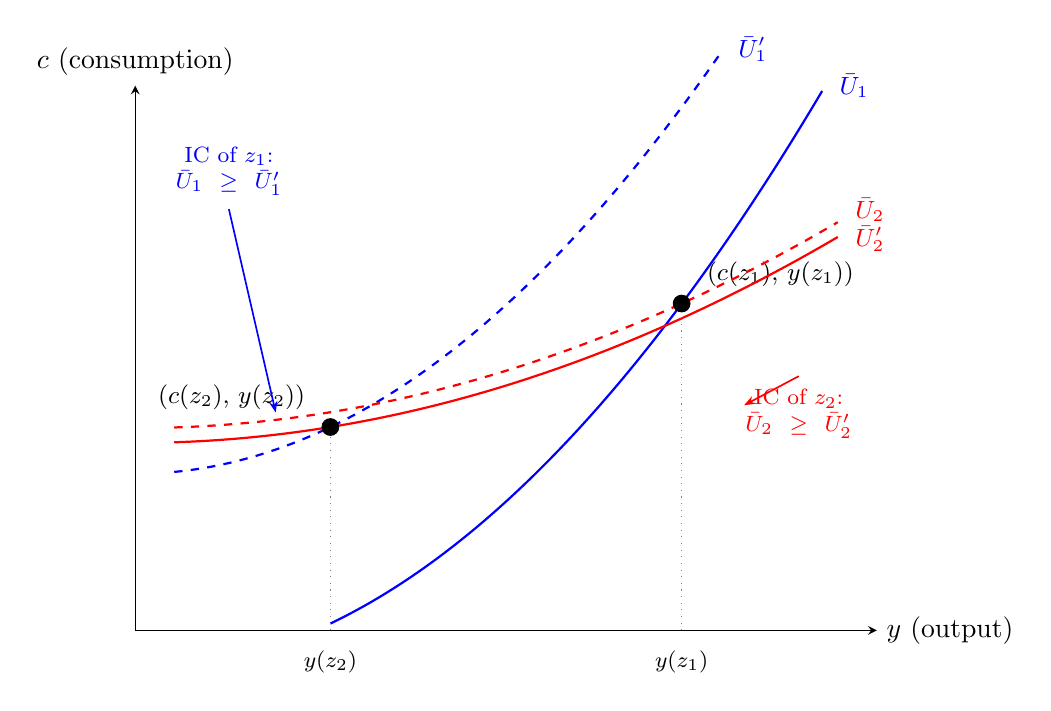
\begin{tikzpicture}
\begin{axis}[
  width=11cm, height=8.5cm,
  xlabel={$y$ (output)},
  ylabel={$c$ (consumption)},
  xmin=0, xmax=9.5,
  ymin=0, ymax=7.5,
  axis lines=left,
  xtick=\empty, ytick=\empty,
  clip=false,
  every axis x label/.style={at={(ticklabel* cs:1)}, anchor=west},
  every axis y label/.style={at={(ticklabel* cs:1)}, anchor=south},
]

% --- Bundle 2: assigned to z_2 (high type), at LOWER y ---
% (y_2, c_2) = (2.5, 2.8)
\addplot[only marks, mark=*, mark size=3pt, black] coordinates {(2.5,2.8)};
\node[font=\small, anchor=south east] at (axis cs:2.3,2.9) {$(c(z_2),\, y(z_2))$};

% --- Bundle 1: assigned to z_1 (low type), at HIGHER y ---
% (y_1, c_1) = (7.0, 4.5)
\addplot[only marks, mark=*, mark size=3pt, black] coordinates {(7.0,4.5)};
\node[font=\small, anchor=south west] at (axis cs:7.2,4.6) {$(c(z_1),\, y(z_1))$};

% --- z_1's IC through bundle 1 (steep, passes through (7.0, 4.5)) ---
% c = -0.55 + 0.103*y^2   => at y=7.0: c = -0.55 + 0.103*49 = 4.497 ~ 4.5
\addplot[thick, blue, domain=2.5:8.8, samples=80]
  {-0.55 + 0.103*x^2};

% --- z_1's IC through bundle 2 (steep, passes through (2.5, 2.8)) ---
% Need IC of z_1 through (2.5, 2.8): c = k + 0.103*y^2
% 2.8 = k + 0.103*6.25 => k = 2.8 - 0.644 = 2.156
\addplot[thick, blue, dashed, domain=0.5:7.5, samples=80]
  {2.156 + 0.103*x^2};

% --- z_2's IC through bundle 2 (flat, passes through (2.5, 2.8)) ---
% c = k + 0.035*y^2   => 2.8 = k + 0.035*6.25 => k = 2.581
\addplot[thick, red, domain=0.5:9.0, samples=80]
  {2.581 + 0.035*x^2};

% --- z_2's IC through bundle 1 (flat, passes through (7.0, 4.5)) ---
% 4.5 = k + 0.035*49 => k = 2.785
\addplot[thick, red, dashed, domain=0.5:9.0, samples=80]
  {2.785 + 0.035*x^2};

% --- Labels for ICs ---
% z_1 solid (through bundle 1): label at right
\node[blue, font=\small, anchor=west] at (axis cs:8.9,7.5) {$\bar U_1$};
% z_1 dashed (through bundle 2): label at right
\node[blue, font=\small, anchor=west] at (axis cs:7.6,8.0) {$\bar U_1'$};

% z_2 solid (through bundle 2): label at right end
\node[red, font=\small, anchor=south west] at (axis cs:9.1,5.5) {$\bar U_2$};
% z_2 dashed (through bundle 1): label at right end
\node[red, font=\small, anchor=north west] at (axis cs:9.1,5.7) {$\bar U_2'$};

% --- Annotations explaining the contradiction ---
% IC of z_1: bundle 1 must be weakly preferred to bundle 2
% => solid blue >= dashed blue (at the z_1 bundle, solid is higher utility)
\draw[blue, -{Stealth[length=4pt]}, semithick] (axis cs:1.2,5.8) -- (axis cs:1.8,3.0);
\node[blue, font=\footnotesize, anchor=south, text width=3.2cm, align=center]
  at (axis cs:1.2,5.85) {IC of $z_1$:\\$\bar U_1 \geq \bar U_1'$};

\draw[red, -{Stealth[length=4pt]}, semithick] (axis cs:8.5,3.5) -- (axis cs:7.8,3.1);
\node[red, font=\footnotesize, anchor=north, text width=3.2cm, align=center]
  at (axis cs:8.5,3.45) {IC of $z_2$:\\$\bar U_2 \geq \bar U_2'$};

% --- Crossing marker ---
% The blue dashed and red solid curves cross between the two bundles
% Blue dashed: 2.156 + 0.103*y^2;  Red solid: 2.581 + 0.035*y^2
% Cross: 2.156 + 0.103*y^2 = 2.581 + 0.035*y^2 => 0.068*y^2 = 0.425 => y = 2.5
% They cross right at bundle 2. The key crossing is between the solid curves:
% Blue solid: -0.55 + 0.103*y^2;  Red dashed: 2.785 + 0.035*y^2
% Cross: 0.068*y^2 = 3.335 => y = 7.0 -- they cross at bundle 1.
% The visual point: between the bundles, the relative ordering of the
% curves for the two types reverses, which is the SC violation.

% --- Vertical guides ---
\addplot[thin, gray, dotted] coordinates {(2.5,0) (2.5,2.8)};
\addplot[thin, gray, dotted] coordinates {(7.0,0) (7.0,4.5)};
\node[anchor=north, font=\footnotesize] at (axis cs:2.5,-0.15) {$y(z_2)$};
\node[anchor=north, font=\footnotesize] at (axis cs:7.0,-0.15) {$y(z_1)$};

\end{axis}
\end{tikzpicture}
\caption{Necessity of monotonicity. Suppose $z_1 < z_2$ but $y(z_1) > y(z_2)$. IC for $z_1$ requires $\bar U_1 \geq \bar U_1'$ (the blue solid curve lies weakly above the blue dashed curve at both bundles). IC for $z_2$ requires $\bar U_2 \geq \bar U_2'$ (red solid weakly above red dashed). But single crossing (Lemma~\ref{lem:SC_slopes}) says $z_1$'s ICs are everywhere steeper than $z_2$'s. At the right bundle, $z_1$'s IC (blue solid) is steep and $z_2$'s IC (red dashed) is flat; at the left bundle, the ordering reverses. The two pairs of ICs must therefore cross between the bundles---contradicting single crossing.}
\label{fig:necessity}
\end{figure}

\medskip

\textbf{Sufficiency.} This is the key direction. We must show that for all $z, \hat z \in [\zlow, \zbar]$:
\[
  \calU(z) \equiv U\!\left(c(z), \frac{y(z)}{z}\right)
  \geq U\!\left(c(\hat z), \frac{y(\hat z)}{z}\right).
\]

\emph{Step 1: Tangency condition from the local IC.}
Dividing the local IC \eqref{eq:local_IC_FOC} by $U_c \cdot y'(s)$ (for points where $y'(s) > 0$; the case $y'(s) = 0$ is handled by continuity), the local IC at type $s$ says that the slope of the allocation schedule in $(c,y)$-space equals the MRS of type~$s$ at the allocated bundle:
\begin{equation}
\label{eq:tangency}
  \frac{c'(s)}{y'(s)} = -\frac{U_n\!\left(c(s), \frac{y(s)}{s}\right)}{s \, U_c\!\left(c(s), \frac{y(s)}{s}\right)}
  = S\bigl(c(s), y(s), s\bigr).
\end{equation}
That is, at each point along the allocation schedule, the schedule is tangent to the indifference curve of the local type (Figure~\ref{fig:tangency}).

\begin{figure}[ht]
\centering
\begin{tikzpicture}
\begin{axis}[
  width=11cm, height=8.5cm,
  xlabel={$y$ (output)},
  ylabel={$c$ (consumption)},
  xmin=0, xmax=9.5,
  ymin=0, ymax=7,
  axis lines=left,
  xtick=\empty, ytick=\empty,
  clip=false,
  every axis x label/.style={at={(ticklabel* cs:1)}, anchor=west},
  every axis y label/.style={at={(ticklabel* cs:1)}, anchor=south},
]

% --- Allocation schedule: c = 1.8*sqrt(y) - 0.6 ---
\addplot[very thick, black, domain=0.5:9, samples=100]
  {1.8*sqrt(x) - 0.6};
% Schedule label: placed at right end of curve
\node[font=\small, anchor=west] at (axis cs:9.1,4.8) {schedule};

% --- Point for z_L at y=1.5: c = 1.8*sqrt(1.5)-0.6 = 1.60 ---
% IC_L tangent: c = 1.049 + 0.245*y^2
\addplot[thick, blue, domain=0.3:3.4, samples=60]
  {1.049 + 0.245*x^2};
\addplot[only marks, mark=*, mark size=2.5pt, black] coordinates {(1.5,1.60)};

% Label for z_L point: below-left
\node[font=\small, anchor=north east] at (axis cs:1.3,1.35) {$\bigl(c(z_L),\, y(z_L)\bigr)$};
% IC_L label: on the right tail of the blue curve
\node[blue, font=\small, anchor=south west] at (axis cs:3.45,3.95) {IC of $z_L$};

% --- Point for z_H at y=7.5: c = 1.8*sqrt(7.5)-0.6 = 4.33 ---
% IC_H tangent: c = 3.096 + 0.02193*y^2
\addplot[thick, red, dashed, domain=3.5:9.2, samples=60]
  {3.096 + 0.02193*x^2};
\addplot[only marks, mark=*, mark size=2.5pt, black] coordinates {(7.5,4.33)};

% Label for z_H point: to the right
\node[font=\small, anchor=north west] at (axis cs:7.65,4.15) {$\bigl(c(z_H),\, y(z_H)\bigr)$};
% IC_H label: at the right tail of the dashed curve, above it
\node[red, font=\small, anchor=south] at (axis cs:8.8,5.95) {IC of $z_H$};

% --- Vertical guides to x-axis ---
\addplot[thin, gray, dotted] coordinates {(1.5,0) (1.5,1.60)};
\addplot[thin, gray, dotted] coordinates {(7.5,0) (7.5,4.33)};
\node[anchor=north, font=\footnotesize] at (axis cs:1.5,-0.15) {$y(z_L)$};
\node[anchor=north, font=\footnotesize] at (axis cs:7.5,-0.15) {$y(z_H)$};

\end{axis}
\end{tikzpicture}
\caption{Step~1: Tangency of the allocation schedule. The allocation schedule (solid black curve) is tangent to each type's indifference curve at the assigned bundle. Type~$z_L$'s IC (blue, solid) is steep at its bundle, while type~$z_H$'s IC (red, dashed) is flat at its bundle, reflecting the single-crossing property.}
\label{fig:tangency}
\end{figure}

\emph{Step 2: Utility of type $z$ along the allocation path.}
For a fixed true type $z$ and variable report $\hat z$, define
\[
  \Phi(\hat z) \equiv U\!\left(c(\hat z), \frac{y(\hat z)}{z}\right).
\]
Note that $\Phi(z) = \calU(z)$. We want to show $\Phi(z) \geq \Phi(\hat z)$ for all $\hat z$, i.e., that $\Phi$ achieves its maximum at $\hat z = z$.

Differentiating $\Phi$ with respect to $\hat z$:
\begin{align}
  \Phi'(\hat z)
  &= U_c\!\left(c(\hat z), \frac{y(\hat z)}{z}\right) c'(\hat z)
     + U_n\!\left(c(\hat z), \frac{y(\hat z)}{z}\right) \frac{y'(\hat z)}{z}.
  \label{eq:Phi_prime_raw}
\end{align}
Factor out $U_c(c(\hat z), y(\hat z)/z) \cdot y'(\hat z)$:
\begin{equation}
\label{eq:Phi_prime}
  \Phi'(\hat z)
  = U_c\!\left(c(\hat z), \frac{y(\hat z)}{z}\right) \cdot y'(\hat z)
     \left[ \frac{c'(\hat z)}{y'(\hat z)} - S\bigl(c(\hat z), y(\hat z), z\bigr) \right].
\end{equation}
Using the tangency condition \eqref{eq:tangency} evaluated at $s = \hat z$ to substitute for $c'(\hat z)/y'(\hat z)$:
\begin{equation}
\label{eq:Phi_prime_SC}
  \Phi'(\hat z)
  = U_c\!\left(c(\hat z), \frac{y(\hat z)}{z}\right) \cdot y'(\hat z)
    \bigl[ S(c(\hat z), y(\hat z), \hat z) \;-\; S(c(\hat z), y(\hat z), z) \bigr].
\end{equation}

\emph{Step 3: Signing $\Phi'$ using single crossing.}
In expression \eqref{eq:Phi_prime_SC}, $U_c > 0$ always, and $y'(\hat z) \geq 0$ by the monotonicity assumption~(ii). By Lemma~\ref{lem:SC_slopes}, $S$ is strictly decreasing in its third argument, so:
\begin{itemize}
  \item If $\hat z < z$: then $S(c(\hat z), y(\hat z), \hat z) > S(c(\hat z), y(\hat z), z)$, so the bracket in \eqref{eq:Phi_prime_SC} is positive, and hence $\Phi'(\hat z) \geq 0$.
  \item If $\hat z > z$: then $S(c(\hat z), y(\hat z), \hat z) < S(c(\hat z), y(\hat z), z)$, so the bracket is negative, and hence $\Phi'(\hat z) \leq 0$.
\end{itemize}
Thus $\Phi$ is nondecreasing for $\hat z < z$ and nonincreasing for $\hat z > z$. It follows that $\Phi$ achieves its maximum at $\hat z = z$:
\[
  \calU(z) = \Phi(z) \geq \Phi(\hat z) = U\!\left(c(\hat z), \frac{y(\hat z)}{z}\right) \quad \text{for all } \hat z. \qedhere
\]
\end{proof}

\begin{remark}[Geometric interpretation]
The proof has an intuitive geometric reading, illustrated in Figure~\ref{fig:deviation}. The allocation schedule traces a curve in $(c,y)$-space. At each point $(c(s), y(s))$, this curve is tangent to type $s$'s indifference curve (Step~1, Figure~\ref{fig:tangency}). Now consider type $z_H$ evaluating the bundle assigned to some lower type $z_L$. By single crossing, type $z_H$ has \emph{flatter} indifference curves than type $z_L$ at any given point. So the allocation schedule---tangent to $z_L$'s steeper indifference curve at the bundle $(c(z_L), y(z_L))$---rises more steeply than $z_H$'s own indifference curves. As type $z_H$ ``walks down'' the allocation schedule toward lower bundles, each step moves to a lower indifference curve for $z_H$: the schedule climbs faster than $z_H$'s indifference curves would require to maintain constant utility. The argument for upward deviations ($z_L$ considering $z_H$'s bundle) is symmetric---the schedule is now \emph{flatter} than $z_L$'s indifference curves.
\end{remark}

\begin{figure}[ht]
\centering
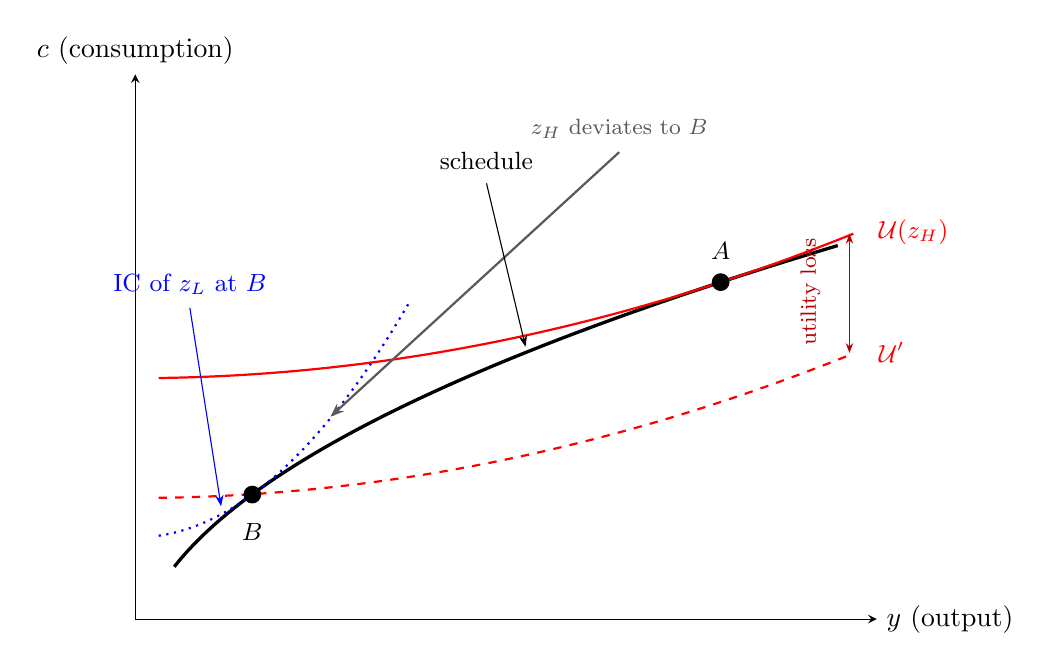
\begin{tikzpicture}
\begin{axis}[
  width=11cm, height=8.5cm,
  xlabel={$y$ (output)},
  ylabel={$c$ (consumption)},
  xmin=0, xmax=9.5,
  ymin=0, ymax=7,
  axis lines=left,
  xtick=\empty, ytick=\empty,
  clip=false,
  every axis x label/.style={at={(ticklabel* cs:1)}, anchor=west},
  every axis y label/.style={at={(ticklabel* cs:1)}, anchor=south},
]

% --- Allocation schedule: c = 1.8*sqrt(y) - 0.6 ---
\addplot[very thick, black, domain=0.5:9, samples=100]
  {1.8*sqrt(x) - 0.6};

% --- Points A (z_H's bundle) and B (z_L's bundle) ---
\addplot[only marks, mark=*, mark size=3pt, black] coordinates {(7.5,4.33)};
\addplot[only marks, mark=*, mark size=3pt, black] coordinates {(1.5,1.60)};
\node[font=\small, anchor=south] at (axis cs:7.5,4.5) {$A$};
\node[font=\small, anchor=north] at (axis cs:1.5,1.35) {$B$};

% --- z_H's IC through A (assigned bundle, higher utility) ---
% c = 3.096 + 0.02193*y^2
\addplot[thick, red, domain=0.3:9.2, samples=80]
  {3.096 + 0.02193*x^2};

% --- z_H's IC through B (deviation bundle, lower utility) ---
% c = 1.556 + 0.02193*y^2
\addplot[thick, red, dashed, domain=0.3:9.2, samples=80]
  {1.556 + 0.02193*x^2};

% --- z_L's IC tangent to schedule at B ---
% c = 1.049 + 0.245*y^2
\addplot[thick, blue, dotted, domain=0.3:3.5, samples=60]
  {1.049 + 0.245*x^2};

% --- Labels placed at edges of figure, away from crossings ---

% Red solid (z_H at A): label on right edge
\node[red, font=\small, anchor=west] at (axis cs:9.4,4.97) {$\calU(z_H)$};

% Red dashed (z_H at B): label on right edge, below
\node[red, font=\small, anchor=west] at (axis cs:9.4,3.43) {$\calU'$};

% Blue dotted (z_L at B): label above, using arrow from clear space
\draw[blue, -{Stealth[length=4pt]}, thin] (axis cs:0.7,4.0) -- (axis cs:1.1,1.45);
\node[blue, font=\small, anchor=south] at (axis cs:0.7,4.05) {IC of $z_L$ at $B$};

% --- Arrow showing deviation direction (placed high, in clear space) ---
\draw[-{Stealth[length=5pt]}, thick, gray!70!black] (axis cs:6.2,6.0) -- (axis cs:2.5,2.6);
\node[gray!70!black, font=\footnotesize, anchor=south] at (axis cs:6.2,6.05) {$z_H$ deviates to $B$};

% --- Double arrow for utility gap (placed at right margin) ---
\draw[red!70!black, {Stealth[length=3.5pt]}-{Stealth[length=3.5pt]}, semithick] 
  (axis cs:9.15,4.95) -- (axis cs:9.15,3.42);
\node[red!70!black, font=\footnotesize, rotate=90, anchor=south] at (axis cs:8.9,4.2) {utility loss};

% Schedule label (placed at top, away from everything)
\draw[black, -{Stealth[length=4pt]}, thin] (axis cs:4.5,5.6) -- (axis cs:5.0,3.5);
\node[font=\small, anchor=south] at (axis cs:4.5,5.65) {schedule};

\end{axis}
\end{tikzpicture}
\caption{Step~3: Why downward deviations are suboptimal. Type~$z_H$ is assigned bundle~$A$ and considers deviating to~$B$ (designed for $z_L$). The solid red curve is $z_H$'s indifference curve through~$A$; the dashed red curve is $z_H$'s (lower) indifference curve through~$B$. At~$B$, the allocation schedule is tangent to $z_L$'s steep IC (blue dotted), so the schedule rises faster than $z_H$'s flat ICs. Walking from~$A$ toward~$B$, the schedule falls below $z_H$'s original IC, producing a utility loss.}
\label{fig:deviation}
\end{figure}


\section{The Classical Runge--Kutta Method (RK4)}
\label{app:rk4}

This appendix derives the classical fourth-order Runge--Kutta method used in both the non-robust (Section~\ref{sec:ode_approach}) and robust (Section~\ref{sec:robust_taxation}) ODE computations. We build up from first-order (Euler) through second-order (RK2) to the full fourth-order method, making the Taylor-matching strategy transparent at each stage.

\subsection{The problem}

Consider an initial value problem (IVP):
\begin{equation}
\label{eq:rk4_ivp}
  \frac{dy}{dt} = f(t, y), \qquad y(t_0) = y_0.
\end{equation}
We want a rule that, given $(t_n, y_n)$, produces $y_{n+1} \approx y(t_n + h)$ with step size $h = t_{n+1} - t_n$.

\paragraph{Forward Euler.} The simplest approach: step along the current slope,
\[
  y_{n+1} = y_n + h\, f(t_n, y_n).
\]
This is first-order: the local truncation error (LTE) is $O(h^2)$, giving a global error $O(h)$. We want to do better by evaluating $f$ at \emph{multiple} points within the step and taking a weighted average.

\subsection{Warmup: deriving the second-order method (RK2)}
%% ================================================================

Following the approach in Zeltkevic (1998), suppose we seek a method of the form
\begin{equation}\label{eq:rk4app_rk2_ansatz}
  \begin{aligned}
    k_1 &= h\, f(t_n, y_n), \\
    k_2 &= h\, f(t_n + \alpha h, \; y_n + \beta\, k_1), \\
    y_{n+1} &= y_n + a\, k_1 + b\, k_2,
  \end{aligned}
\end{equation}
where $\alpha, \beta, a, b$ are constants to be determined so that the LTE is $O(h^3)$.

\subsubsection{Taylor expansion of the exact solution}

Expand $y(t_n + h)$ around $t_n$:
\begin{equation}\label{eq:rk4app_taylor2}
  y(t_n + h) = y_n + h\,\frac{dy}{dt} + \frac{h^2}{2}\,\frac{d^2 y}{dt^2} + O(h^3).
\end{equation}
Since $dy/dt = f$, the chain rule gives
\begin{equation}\label{eq:rk4app_d2y}
  \frac{d^2 y}{dt^2} = \frac{df}{dt} = f_t + f_y \cdot f,
\end{equation}
where all partials are evaluated at $(t_n, y_n)$. So
\begin{equation}\label{eq:rk4app_exact2}
  y(t_n + h) = y_n + h\,f + \frac{h^2}{2}\big(f_t + f\, f_y\big) + O(h^3).
\end{equation}

\subsubsection{Taylor expansion of the RK2 ansatz}

Expand $k_2$ using a two-variable Taylor expansion of $f$:
\begin{align}
  k_2 &= h\,f\big(t_n + \alpha h, \; y_n + \beta\, k_1\big) \notag\\
      &= h\left[f + \alpha h\, f_t + \beta\, k_1\, f_y + O(h^2)\right] \notag\\
      &= h\,f + h^2\big(\alpha\, f_t + \beta\, f\, f_y\big) + O(h^3). \label{eq:rk4app_k2_expand}
\end{align}
Substituting into $y_{n+1} = y_n + a\,k_1 + b\,k_2$:
\begin{equation}\label{eq:rk4app_rk2_expand}
  y_{n+1} = y_n + (a+b)\,h\,f + b\,h^2\big(\alpha\, f_t + \beta\, f\, f_y\big) + O(h^3).
\end{equation}

\subsubsection{Matching coefficients}

Comparing \eqref{eq:rk4app_exact2} and \eqref{eq:rk4app_rk2_expand} term by term:
\begin{equation}\label{eq:rk4app_rk2_conditions}
  \boxed{a + b = 1, \qquad b\,\alpha = \frac{1}{2}, \qquad b\,\beta = \frac{1}{2}.}
\end{equation}
Three equations, four unknowns: a one-parameter family. The common choice $\alpha = \beta = 1$, $a = b = 1/2$ gives the \textbf{classical RK2} (also called the improved Euler or Heun method):
\begin{equation}
  y_{n+1} = y_n + \frac{1}{2}(k_1 + k_2), \qquad k_2 = h\,f(t_n + h, \, y_n + k_1).
\end{equation}

%% ================================================================
\subsection{Geometric intuition}
%% ================================================================

\subsubsection{Why RK2 improves on Euler}

The problem with Euler's method is that it commits to the slope at $t_n$ for the entire step. If the slope is changing (i.e., $f$ is not constant), this produces a systematic drift. RK2 fixes this by using the Euler step as a \emph{probe}: it takes a trial step to $t_n + h$ to estimate the slope there, then averages the two slopes.

\begin{figure}[ht]
\centering
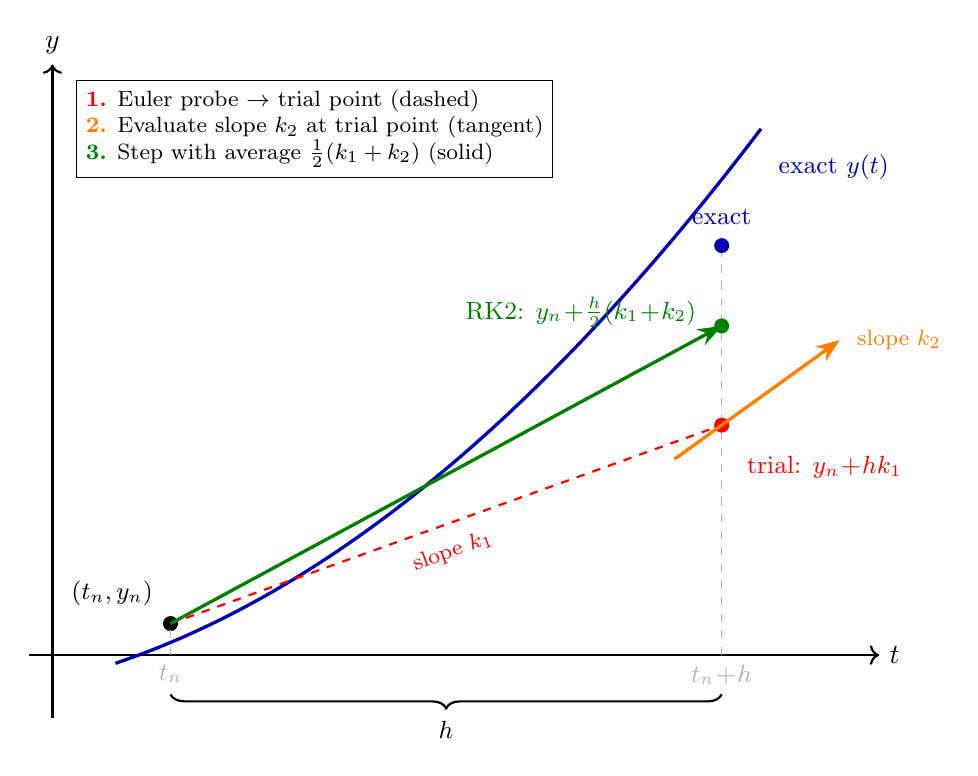
\begin{tikzpicture}[scale=1.0]
  % Axes
  \draw[->,thick] (-0.3,0) -- (10.5,0) node[right] {$t$};
  \draw[->,thick] (0,-0.8) -- (0,7.5) node[above] {$y$};

  % Exact solution curve (steeper to separate points vertically)
  \draw[blue!70!black, very thick, domain=0.8:9.0, samples=100]
    plot (\x, {-0.2 + 0.3*(\x-0.5) + 0.06*(\x-0.5)^2});
  \node[blue!70!black, font=\small, anchor=west] at (9.1,6.2) {exact $y(t)$};

  % Starting point at (1.5, 0.4)
  \filldraw[black] (1.5, 0.4) circle (2.5pt);
  \node[above left, font=\small] at (1.4, 0.5) {$(t_n, y_n)$};

  % Time markers
  \draw[dashed, gray!60] (1.5,0) node[below, font=\small] {$t_n$} -- (1.5,0.4);
  \draw[dashed, gray!60] (8.5,0) node[below, font=\small] {$t_n\!+\!h$} -- (8.5,5.2);

  % Exact value at t_n+h = 5.2
  \filldraw[blue!70!black] (8.5, 5.2) circle (2.5pt);
  \node[blue!70!black, font=\small, anchor=south] at (8.5, 5.35) {exact};

  % === Step 1: Euler probe ===
  % slope k1 = 0.36, rise over 7 units = 2.52, endpoint y = 0.4+2.52 = 2.92
  \draw[red, thick, dashed] (1.5, 0.4) -- (8.5, 2.92);
  \filldraw[red] (8.5, 2.92) circle (2.5pt);
  % k1 slope label: below the dashed line, rotated to follow it
  \node[red, font=\footnotesize, rotate=20, anchor=north] at (5.0, 1.55)
    {slope $k_1$};

  % === Step 2: k2 tangent at trial point ===
  % k2 slope ~ 0.72, draw tangent only to the right to avoid crossing other elements
  \draw[orange, very thick, -{Stealth[length=3mm]}]
    (8.5, 2.92) -- ({8.5 + 1.5}, {2.92 + 1.5*0.72});
  % Also draw a short stub to the left
  \draw[orange, very thick]
    ({8.5 - 0.6}, {2.92 - 0.6*0.72}) -- (8.5, 2.92);
  % Label at arrowhead
  \node[orange, font=\footnotesize, anchor=west] at (10.1, {2.92 + 1.5*0.72})
    {slope $k_2$};

  % Trial point label: below-right, well clear of the tangent
  \node[red, font=\small, anchor=north west] at (8.7, 2.65) {trial: $y_n\!+\!hk_1$};

  % === Step 3: RK2 result ===
  % avg slope = (0.36+0.72)/2 = 0.54, rise = 7*0.54 = 3.78, endpoint y = 0.4+3.78 = 4.18
  \draw[green!50!black, very thick, -{Stealth[length=3mm]}] (1.5, 0.4) -- (8.5, 4.18);
  \filldraw[green!50!black] (8.5, 4.18) circle (2.5pt);
  % Label to the left, vertically centered on the dot
  \node[green!50!black, font=\small, anchor=east] at (8.3, 4.35)
    {RK2: $y_n\!+\!\tfrac{h}{2}(k_1\!+\!k_2)$};

  % Brace for h
  \draw[decorate, decoration={brace, amplitude=5pt, mirror}, thick]
    (1.5, -0.5) -- (8.5, -0.5) node[midway, below=6pt, font=\small] {$h$};

  % Legend box (top left, well clear)
  \node[draw, fill=white, font=\footnotesize, align=left, anchor=north west] at (0.3, 7.3) {
    \textcolor{red}{\textbf{1.}} Euler probe $\to$ trial point (dashed)\\
    \textcolor{orange}{\textbf{2.}} Evaluate slope $k_2$ at trial point (tangent)\\
    \textcolor{green!50!black}{\textbf{3.}} Step with average $\frac{1}{2}(k_1+k_2)$ (solid)
  };

\end{tikzpicture}
\caption{Why RK2 beats Euler. \textbf{Step~1} (red dashed): take a trial Euler step using the slope $k_1$ at $t_n$, arriving at the trial point. \textbf{Step~2} (orange tangent): evaluate the slope $k_2$ at the trial point---it is steeper because the solution curves upward. \textbf{Step~3} (green solid): step from $(t_n, y_n)$ using the average slope $\frac{1}{2}(k_1 + k_2)$, which corrects for the curvature and lands close to the exact solution.}
\label{fig:rk2_geometry}
\end{figure}

Algebraically, this is exactly what the matching conditions enforce: the $b\alpha = 1/2$ condition ensures the method captures the $h^2$ term $\frac{1}{2}(f_t + ff_y)$ from the Taylor expansion---the first correction for curvature.

\subsubsection{From RK2 to RK4}

Before diving into the algebra for RK4, consider the geometry.

\begin{figure}[ht]
\centering
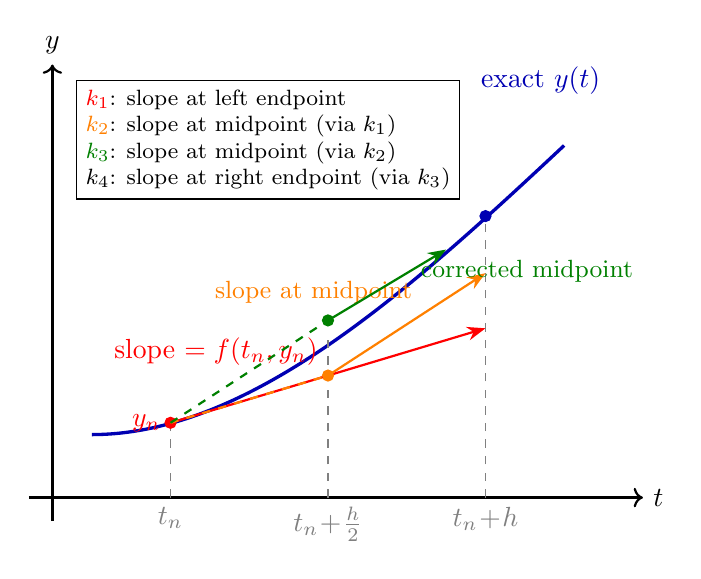
\begin{tikzpicture}[scale=1.0]
  % Axes
  \draw[->,thick] (-0.3,0) -- (7.5,0) node[right] {$t$};
  \draw[->,thick] (0,-0.3) -- (0,5.5) node[above] {$y$};
  
  % Exact solution curve (a nice exponential-like curve)
  \draw[blue!70!black, very thick, domain=0.5:6.5, samples=100] 
    plot (\x, {0.8 + 0.15*(\x-0.5)^2 - 0.008*(\x-0.5)^3});
  \node[blue!70!black, above] at (6.2,5.0) {exact $y(t)$};
  
  % Points
  \coordinate (A) at (1.5, 0.95);
  \coordinate (B) at (5.5, 3.575);
  
  % t_n and t_{n+1} labels
  \draw[dashed, gray] (1.5,0) node[below] {$t_n$} -- (A);
  \draw[dashed, gray] (5.5,0) node[below] {$t_n\!+\!h$} -- (B);
  \draw[dashed, gray] (3.5,0) node[below] {$t_n\!+\!\frac{h}{2}$} -- (3.5,2.1);
  
  % Euler step (k1 slope)
  \draw[red, thick, -{Stealth}] (A) -- ++(4, 4*0.3) 
    node[pos=0.5, above left, red] {slope $= f(t_n,y_n)$};
  \filldraw[red] (A) circle (2pt) node[left] {$y_n$};
  
  % Midpoint evaluation
  \draw[orange, thick, dashed] (A) -- ++(2, 2*0.3);
  \filldraw[orange] (3.5, 1.55) circle (2pt);
  \draw[orange, thick, -{Stealth}] (3.5, 1.55) -- ++(2, 2*0.65) 
    node[pos=0.6, above left, orange, font=\small] {slope at midpoint};
  
  % k3 corrected midpoint
  \draw[green!50!black, thick, dashed] (A) -- ++(2, 2*0.65);
  \filldraw[green!50!black] (3.5, 2.25) circle (2pt);
  \draw[green!50!black, thick, -{Stealth}] (3.5, 2.25) -- ++(1.5, 1.5*0.6)
    node[pos=0.7, right, green!50!black, font=\small] {corrected midpoint};
  
  % Exact value
  \filldraw[blue!70!black] (B) circle (2pt);
  
  % Legend box
  \node[draw, fill=white, font=\footnotesize, align=left, anchor=north west] at (0.3, 5.3) {
    \textcolor{red}{$k_1$}: slope at left endpoint\\
    \textcolor{orange}{$k_2$}: slope at midpoint (via $k_1$)\\
    \textcolor{green!50!black}{$k_3$}: slope at midpoint (via $k_2$)\\
    $k_4$: slope at right endpoint (via $k_3$)
  };
\end{tikzpicture}
\caption{Geometric idea behind RK4. Euler uses one slope (red). RK4 evaluates the slope at four points and takes a weighted average, achieving much higher accuracy per step.}
\label{fig:geometry}
\end{figure}

The key idea: Euler's method uses only the slope at $t_n$. RK4 samples the slope at four points---the left endpoint, two midpoint estimates, and the right endpoint---then combines them with Simpson's-rule weights $(1,2,2,1)/6$.

%% ================================================================
\subsection{Deriving the fourth-order method (RK4)}
%% ================================================================

\subsubsection{The ansatz}

We now seek a 4-stage method:
\begin{equation}\label{eq:rk4app_rk4_ansatz}
  \begin{aligned}
    k_1 &= f(t_n, \, y_n), \\
    k_2 &= f\big(t_n + c_2 h, \; y_n + h\, a_{21}\, k_1\big), \\
    k_3 &= f\big(t_n + c_3 h, \; y_n + h(a_{31}\, k_1 + a_{32}\, k_2)\big), \\
    k_4 &= f\big(t_n + c_4 h, \; y_n + h(a_{41}\, k_1 + a_{42}\, k_2 + a_{43}\, k_3)\big), \\
    y_{n+1} &= y_n + h\big(b_1\, k_1 + b_2\, k_2 + b_3\, k_3 + b_4\, k_4\big),
  \end{aligned}
\end{equation}
with consistency conditions $c_i = \sum_j a_{ij}$ and 10 free parameters. We require the LTE to be $O(h^5)$.

The strategy is identical to the RK2 derivation above: expand everything in Taylor series, match coefficients with the exact solution, and solve the resulting algebraic system.

\subsubsection{Taylor expansion of the exact solution through $O(h^4)$}

We need $y',\, y'',\, y''',\, y^{(4)}$:
\begin{align}
  y' &= f, \label{eq:rk4app_y1}\\
  y'' &= f_t + f_y\, f \;\equiv\; Df, \label{eq:rk4app_y2}\\
  y''' &= D^2f = f_{tt} + 2f_{ty}\,f + f_{yy}\,f^2 + f_y\, Df, \label{eq:rk4app_y3}\\
  y^{(4)} &= D^3f \quad\text{(see below)}, \label{eq:rk4app_y4}
\end{align}
where $D = \partial_t + f\,\partial_y$ is the total derivative operator along solutions. Hence:
\begin{equation}\label{eq:rk4app_exact4}
  y(t_n + h) = y_n + hf + \frac{h^2}{2}Df + \frac{h^3}{6}D^2f + \frac{h^4}{24}D^3f + O(h^5).
\end{equation}

\subsubsection{Taylor expansion of the stages}

This proceeds exactly as in the RK2 case, but now we need the two-variable Taylor expansion through higher order. Write $\Delta t_i = c_i h$ and $\Delta y_i = h \sum_j a_{ij} k_j$ for the perturbation in each stage.

\paragraph{Stage 2.} Expanding to $O(h^2)$:
\begin{equation}
  k_2 = f + c_2 h\,(f_t + f_y f) + \frac{c_2^2 h^2}{2}(f_{tt} + 2f\,f_{ty} + f^2 f_{yy}) + O(h^3).
\end{equation}

\paragraph{Stages 3 and 4.} The expansions are analogous but involve substituting the expansion of earlier stages. For example, in $k_3$ the perturbation $\Delta y_3 = h(a_{31}k_1 + a_{32}k_2)$ contains $k_2$, which itself has $O(h)$ corrections. This coupling is what generates the additional order conditions beyond simple quadrature.

\subsubsection{The eight order conditions}

Substituting the stage expansions into $y_{n+1}$ and comparing with \eqref{eq:rk4app_exact4} order by order yields 8 algebraic conditions. We state them using the compact Butcher notation $\sum_i b_i (\cdots)$:

\medskip

\noindent\textbf{Order 1} (1 condition, from the $h$ coefficient):
\begin{equation}\label{eq:rk4app_oc1}
  \sum_i b_i = 1.
\end{equation}

\noindent\textbf{Order 2} (1 condition, from the $h^2$ coefficient):
\begin{equation}\label{eq:rk4app_oc2}
  \sum_i b_i\, c_i = \frac{1}{2}.
\end{equation}

\noindent\textbf{Order 3} (2 conditions, from the two distinct terms in $D^2f$):
\begin{equation}\label{eq:rk4app_oc3}
  \sum_i b_i\, c_i^2 = \frac{1}{3}, \qquad \sum_i b_i \sum_j a_{ij}\, c_j = \frac{1}{6}.
\end{equation}

\noindent\textbf{Order 4} (4 conditions, from the four distinct terms in $D^3f$):
\begin{align}
  \sum_i b_i\, c_i^3 &= \frac{1}{4}, \label{eq:rk4app_oc4a}\\
  \sum_i b_i\, c_i \sum_j a_{ij}\, c_j &= \frac{1}{8}, \label{eq:rk4app_oc4b}\\
  \sum_i b_i \sum_j a_{ij}\, c_j^2 &= \frac{1}{12}, \label{eq:rk4app_oc4c}\\
  \sum_i b_i \sum_j a_{ij} \sum_k a_{jk}\, c_k &= \frac{1}{24}. \label{eq:rk4app_oc4d}
\end{align}

\begin{remark}
The right-hand sides $1, \tfrac{1}{2}, \tfrac{1}{3}, \tfrac{1}{6}, \ldots$ are exactly $1/\sigma(\tau)$ for each rooted tree $\tau$---the reciprocal of the tree's ``density'' in Butcher's formalism. The number of conditions at each order equals the number of rooted trees: $1, 1, 2, 4$ at orders $1,2,3,4$.
\end{remark}

\subsubsection{Solving the system: the classical choice}

We have 8 equations in 10 unknowns, leaving a 2-parameter family. The \textbf{classical RK4} uses the symmetric node placement
\[
  c_1 = 0, \qquad c_2 = c_3 = \tfrac{1}{2}, \qquad c_4 = 1,
\]
and further requires that each stage uses only the \emph{most recent} slope estimate:
\[
  a_{31} = 0 \;\;(\text{skip } k_1), \qquad a_{41} = a_{42} = 0 \;\;(\text{skip } k_1, k_2).
\]

Under these simplifications, the system solves uniquely:

\paragraph{From consistency:} $a_{21} = \tfrac{1}{2}$, $a_{32} = \tfrac{1}{2}$, $a_{43} = 1$.

\paragraph{From \eqref{eq:rk4app_oc4d}:} $b_4 \cdot 1 \cdot \tfrac{1}{2} \cdot \tfrac{1}{2} = \tfrac{1}{24}$ $\implies$ $b_4 = \tfrac{1}{6}$.

\paragraph{From \eqref{eq:rk4app_oc4c}:} $b_3 \cdot \tfrac{1}{2} \cdot \tfrac{1}{4} + \tfrac{1}{6}\cdot 1 \cdot \tfrac{1}{4} = \tfrac{1}{12}$ $\implies$ $b_3 = \tfrac{1}{3}$.

\paragraph{From \eqref{eq:rk4app_oc3}$_1$:} $b_2 \cdot \tfrac{1}{4} + \tfrac{1}{3}\cdot\tfrac{1}{4} + \tfrac{1}{6}\cdot 1 = \tfrac{1}{3}$ $\implies$ $b_2 = \tfrac{1}{3}$.

\paragraph{From \eqref{eq:rk4app_oc1}:} $b_1 = 1 - \tfrac{1}{3} - \tfrac{1}{3} - \tfrac{1}{6} = \tfrac{1}{6}$.

One can verify that the remaining conditions \eqref{eq:rk4app_oc2}, \eqref{eq:rk4app_oc3}$_2$, \eqref{eq:rk4app_oc4a}, \eqref{eq:rk4app_oc4b} are all satisfied. The Butcher tableau is:
\[
  \begin{array}{c|cccc}
    0 \\[2pt]
    \frac{1}{2} & \frac{1}{2} \\[2pt]
    \frac{1}{2} & 0 & \frac{1}{2} \\[2pt]
    1 & 0 & 0 & 1 \\[2pt]
    \hline
    \\[-8pt]
    & \frac{1}{6} & \frac{1}{3} & \frac{1}{3} & \frac{1}{6}
  \end{array}
\]

%% ================================================================
\subsection{The algorithm}
%% ================================================================

\begin{proposition}[RK4 convergence]
\label{prop:rk4_convergence}
The method
\begin{align*}
  k_1 &= f(t_n,\, y_n), \\
  k_2 &= f\!\left(t_n + \tfrac{h}{2},\; y_n + \tfrac{h}{2}\,k_1\right), \\
  k_3 &= f\!\left(t_n + \tfrac{h}{2},\; y_n + \tfrac{h}{2}\,k_2\right), \\
  k_4 &= f\!\left(t_n + h,\; y_n + h\,k_3\right), \\[4pt]
  y_{n+1} &= y_n + \tfrac{h}{6}\big(k_1 + 2k_2 + 2k_3 + k_4\big),
\end{align*}
has local truncation error $O(h^5)$ and global error $O(h^4)$, provided $f \in C^4$.
\end{proposition}

%% ================================================================
\subsection{Numerical illustration}
%% ================================================================

Consider the test problem $y' = -y$, $y(0) = 1$, with exact solution $y(t) = e^{-t}$.

\subsubsection{Comparing Euler, RK2, and RK4}

\begin{figure}[ht]
\centering
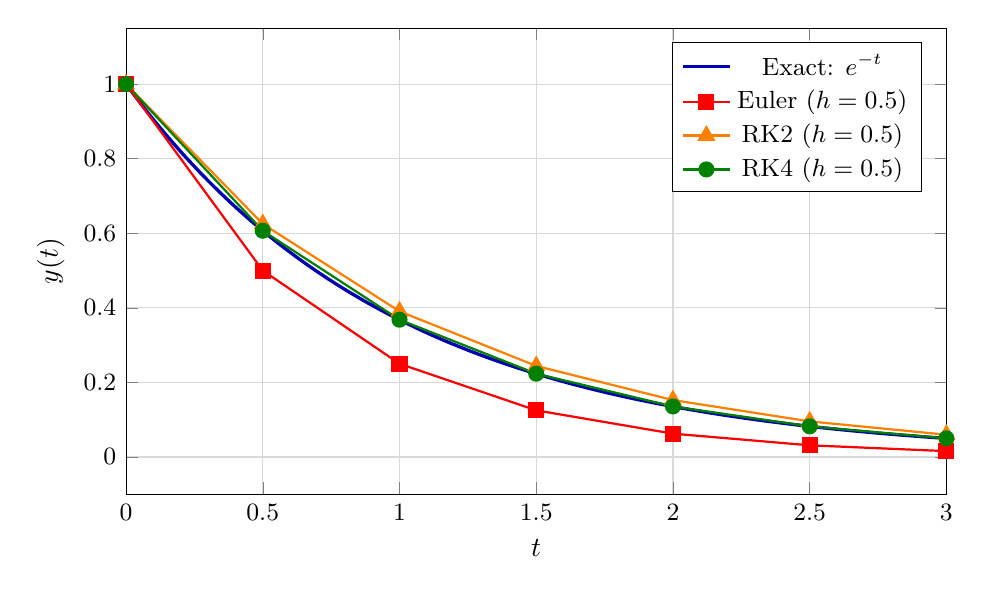
\begin{tikzpicture}
\begin{axis}[
  width=12cm, height=7.5cm,
  xlabel={$t$}, ylabel={$y(t)$},
  xmin=0, xmax=3, ymin=-0.1, ymax=1.15,
  legend pos=north east,
  grid=major,
  grid style={gray!30},
  tick label style={font=\small},
  legend style={font=\small},
]
  % Exact solution
  \addplot[blue!70!black, very thick, domain=0:3, samples=200] {exp(-x)};
  \addlegendentry{Exact: $e^{-t}$}
  
  % Forward Euler with h=0.5
  % y_{n+1} = y_n + h*(-y_n) = y_n(1-h) = y_n * 0.5
  % t=0: y=1, t=0.5: 0.5, t=1: 0.25, t=1.5: 0.125, t=2: 0.0625, t=2.5: 0.03125, t=3: 0.015625
  \addplot[red, thick, mark=square*, mark size=2.5] coordinates {
    (0, 1) (0.5, 0.5) (1.0, 0.25) (1.5, 0.125) (2.0, 0.0625) (2.5, 0.03125) (3.0, 0.015625)
  };
  \addlegendentry{Euler ($h=0.5$)}
  
  % RK2 with h=0.5 (Heun's method)
  % k1 = h*(-y_n) = -0.5*y_n
  % k2 = h*(-(y_n + k1)) = -0.5*(y_n - 0.5*y_n) = -0.5*0.5*y_n = -0.25*y_n
  % y_{n+1} = y_n + 0.5*(k1+k2) = y_n + 0.5*(-0.5*y_n - 0.25*y_n) = y_n*(1 - 0.375) = 0.625*y_n
  % t=0: 1, 0.5: 0.625, 1: 0.390625, 1.5: 0.244140625, 2: 0.152587891, 2.5: 0.095367432, 3: 0.059604645
  \addplot[orange, thick, mark=triangle*, mark size=3] coordinates {
    (0, 1) (0.5, 0.625) (1.0, 0.390625) (1.5, 0.244141) (2.0, 0.152588) (2.5, 0.095367) (3.0, 0.059605)
  };
  \addlegendentry{RK2 ($h=0.5$)}
  
  % RK4 with h=0.5 for y' = -y
  % k1 = -y_n
  % k2 = -(y_n + 0.5*h*k1) = -(y_n - 0.25*y_n) = -0.75*y_n
  % k3 = -(y_n + 0.5*h*k2) = -(y_n - 0.1875*y_n) = -0.8125*y_n
  % k4 = -(y_n + h*k3) = -(y_n - 0.40625*y_n) = -0.59375*y_n
  % y_{n+1} = y_n + (h/6)*(k1 + 2*k2 + 2*k3 + k4)
  %         = y_n + (0.5/6)*(-y_n - 1.5*y_n - 1.625*y_n - 0.59375*y_n)
  %         = y_n + (0.5/6)*(-4.71875*y_n)
  %         = y_n * (1 - 0.5*4.71875/6)
  %         = y_n * (1 - 0.393229)
  %         = y_n * 0.606771
  % Exact: e^{-0.5} = 0.606531
  % t=0: 1, 0.5: 0.606771, 1.0: 0.368171, 1.5: 0.223354, 2.0: 0.135497, 2.5: 0.082211, 3.0: 0.049889
  \addplot[green!50!black, thick, mark=*, mark size=2.5] coordinates {
    (0, 1) (0.5, 0.606771) (1.0, 0.368171) (1.5, 0.223354) (2.0, 0.135497) (2.5, 0.082211) (3.0, 0.049889)
  };
  \addlegendentry{RK4 ($h=0.5$)}
  
\end{axis}
\end{tikzpicture}
\caption{Solution of $y' = -y$, $y(0)=1$ with step size $h = 0.5$. Even at this coarse step size, RK4 is nearly indistinguishable from the exact solution. Euler accumulates visible error; RK2 is intermediate.}
\label{fig:comparison}
\end{figure}

\subsubsection{Convergence rates}

\begin{figure}[ht]
\centering
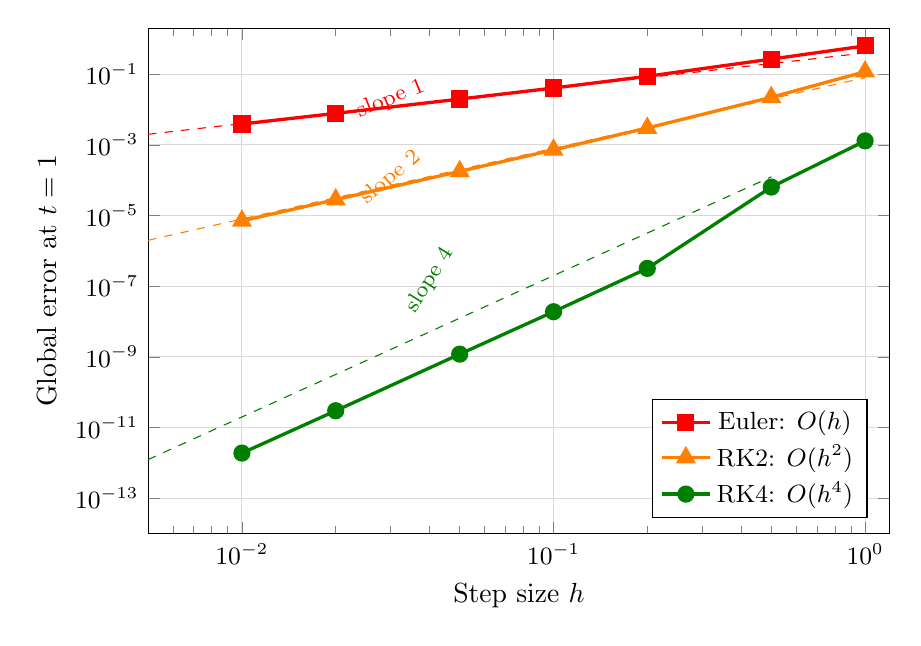
\begin{tikzpicture}
\begin{loglogaxis}[
  width=11cm, height=8cm,
  xlabel={Step size $h$},
  ylabel={Global error at $t = 1$},
  xmin=0.005, xmax=1.2,
  ymin=1e-14, ymax=2,
  grid=major,
  grid style={gray!30},
  tick label style={font=\small},
  legend pos=south east,
  legend style={font=\small},
]
  % Euler: error ~ C*h, with e^{-1} ~ 0.3679
  % Error = |y_numerical - e^{-1}| at t=1
  % For y'=-y with Euler: y_N = (1-h)^{1/h}, error ~ 0.18*h for small h
  \addplot[red, very thick, mark=square*, mark size=2.5] coordinates {
    (1.0, 0.6321)
    (0.5, 0.2679)
    (0.2, 0.0873)
    (0.1, 0.0406)
    (0.05, 0.0198)
    (0.02, 0.0078)
    (0.01, 0.0039)
  };
  \addlegendentry{Euler: $O(h)$}
  
  % RK2: error ~ C*h^2
  % (1-h)^{1/h} for Heun with multiplier (1 - h + h^2/2)^{1/h}
  \addplot[orange, very thick, mark=triangle*, mark size=3] coordinates {
    (1.0, 0.1179)
    (0.5, 0.0222)
    (0.2, 0.0030)
    (0.1, 0.00072)
    (0.05, 0.000178)
    (0.02, 0.0000283)
    (0.01, 0.00000707)
  };
  \addlegendentry{RK2: $O(h^2)$}
  
  % RK4: error ~ C*h^4
  \addplot[green!50!black, very thick, mark=*, mark size=2.5] coordinates {
    (1.0, 0.0013)
    (0.5, 0.0000640)
    (0.2, 3.2e-7)
    (0.1, 1.9e-8)
    (0.05, 1.2e-9)
    (0.02, 3.0e-11)
    (0.01, 1.9e-12)
  };
  \addlegendentry{RK4: $O(h^4)$}
  
  % Reference slopes
  \addplot[red, dashed, thin, domain=0.005:1] {0.4*x};
  \addplot[orange, dashed, thin, domain=0.005:1] {0.08*x^2};
  \addplot[green!50!black, dashed, thin, domain=0.005:0.5] {0.002*x^4};
  
  % Slope labels
  \node[red, font=\footnotesize, rotate=22] at (axis cs:0.03,0.02) {slope 1};
  \node[orange, font=\footnotesize, rotate=40] at (axis cs:0.03,0.00012) {slope 2};
  \node[green!50!black, font=\footnotesize, rotate=58] at (axis cs:0.04,1.5e-7) {slope 4};
  
\end{loglogaxis}
\end{tikzpicture}
\caption{Log-log plot of global error at $t=1$ versus step size $h$ for $y'=-y$. The slopes confirm: Euler is $O(h)$, RK2 is $O(h^2)$, and RK4 is $O(h^4)$. Halving $h$ reduces the RK4 error by a factor of $2^4 = 16$.}
\label{fig:convergence}
\end{figure}

The convergence plot (Figure~\ref{fig:convergence}) makes the practical payoff vivid. At $h = 0.01$, the Euler error is roughly $10^{-3}$, while RK4 achieves $10^{-12}$---a nine-order-of-magnitude improvement.

%% ================================================================
\subsection{The stages, geometrically}
%% ================================================================

\begin{figure}[ht]
\centering
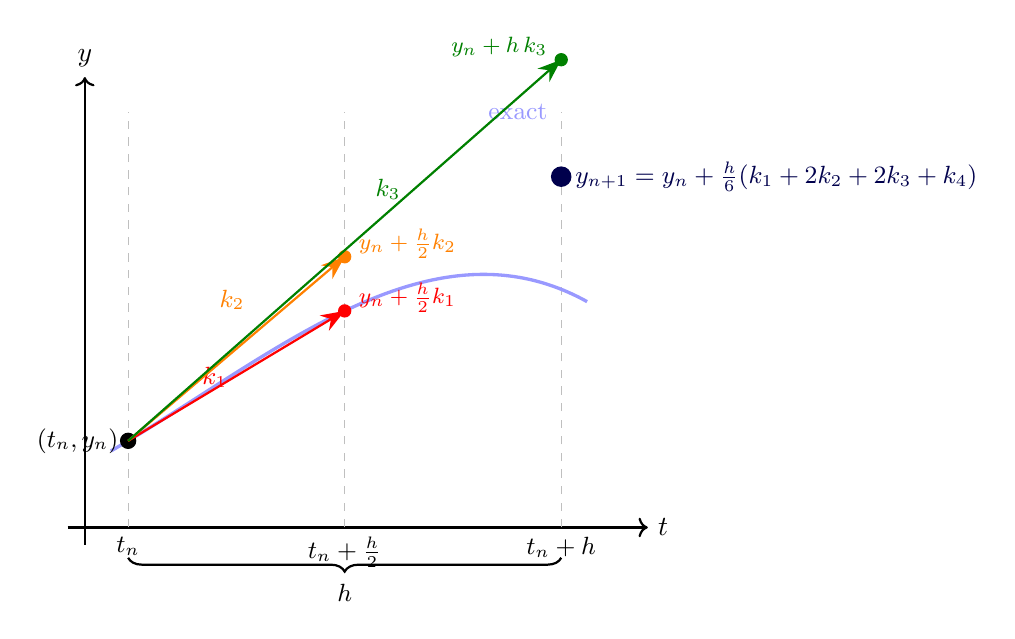
\begin{tikzpicture}[scale=1.1]
  % Setup
  \def\tn{0.5}
  \def\tnph{5.5}
  \def\tmid{3.0}
  \def\yn{1.0}
  \def\h{5.0}
  
  % Axes
  \draw[->,thick] (-0.2,0) -- (6.5,0) node[right] {$t$};
  \draw[->,thick] (0,-0.2) -- (0,5.2) node[above] {$y$};
  
  % Time markers
  \draw[dashed, gray!50] (\tn, 0) -- (\tn, 4.8);
  \draw[dashed, gray!50] (\tmid, 0) -- (\tmid, 4.8);
  \draw[dashed, gray!50] (\tnph, 0) -- (\tnph, 4.8);
  \node[below, font=\small] at (\tn, 0) {$t_n$};
  \node[below, font=\small] at (\tmid, 0) {$t_n + \frac{h}{2}$};
  \node[below, font=\small] at (\tnph, 0) {$t_n + h$};
  
  % Exact curve
  \draw[blue!40, very thick, domain=0.3:5.8, samples=100] 
    plot (\x, {1.0 + 0.6*(\x-0.5) + 0.05*(\x-0.5)^2 - 0.02*(\x-0.5)^3});
  \node[blue!40, font=\small] at (5.0, 4.8) {exact};
  
  % Starting point
  \filldraw[black] (\tn, \yn) circle (2.5pt);
  \node[left, font=\small] at (\tn, \yn) {$(t_n, y_n)$};
  
  % === k1: slope at left ===
  \def\slopeOne{0.6}  % f(t_n, y_n)
  \draw[red, thick, -{Stealth[length=3mm]}] (\tn, \yn) -- 
    (\tmid, {\yn + 2.5*\slopeOne});
  \filldraw[red] (\tmid, {\yn + 2.5*\slopeOne}) circle (2pt);
  \node[red, right, font=\footnotesize] at (\tmid+0.05, {\yn + 2.5*\slopeOne + 0.15}) 
    {$y_n + \frac{h}{2}k_1$};
  \node[red, font=\small, anchor=south] at (1.5, 1.5) {$k_1$};
  
  % === k2: slope at first midpoint ===
  \def\slopeTwo{0.85}
  \draw[orange, thick, -{Stealth[length=3mm]}] (\tn, \yn) -- 
    (\tmid, {\yn + 2.5*\slopeTwo});
  \filldraw[orange] (\tmid, {\yn + 2.5*\slopeTwo}) circle (2pt);
  \node[orange, right, font=\footnotesize] at (\tmid+0.05, {\yn + 2.5*\slopeTwo + 0.15}) 
    {$y_n + \frac{h}{2}k_2$};
  \node[orange, font=\small, anchor=south] at (1.7, 2.4) {$k_2$};
  
  % === k3: slope at corrected midpoint ===
  \def\slopeThree{0.88}
  \draw[green!50!black, thick, -{Stealth[length=3mm]}] (\tn, \yn) -- 
    (\tnph, {\yn + 5.0*\slopeThree});
  \filldraw[green!50!black] (\tnph, {\yn + 5.0*\slopeThree}) circle (2pt);
  \node[green!50!black, left, font=\footnotesize] at (\tnph-0.05, {\yn + 5.0*\slopeThree + 0.15}) 
    {$y_n + h\,k_3$};
  \node[green!50!black, font=\small] at (3.5, 3.9) {$k_3$};
  
  % === Weighted average (RK4 result) ===
  % Approximate final value
  \def\yfinal{4.05}
  \filldraw[black!70!blue, thick] (\tnph, \yfinal) circle (3pt);
  \node[right, font=\small, black!70!blue] at (\tnph+0.05, \yfinal) 
    {$y_{n+1} = y_n + \frac{h}{6}(k_1 + 2k_2 + 2k_3 + k_4)$};
  
  % Brace for h
  \draw[decorate, decoration={brace, amplitude=5pt, mirror}, thick]
    (\tn, -0.35) -- (\tnph, -0.35) node[midway, below=6pt, font=\small] {$h$};
  
\end{tikzpicture}
\caption{The four stages of RK4. Starting from $(t_n, y_n)$: $k_1$ gives a preliminary midpoint via the initial slope; $k_2$ re-evaluates at that midpoint; $k_3$ uses the corrected midpoint slope to step all the way to $t_n + h$, producing the evaluation point for $k_4$. The final result is a weighted average.}
\label{fig:stages}
\end{figure}

%% ================================================================
\subsection{Why not order 5 with 4 stages?}
%% ================================================================

At order $p$, the number of conditions equals the number of rooted trees of order $\leq p$, while the number of free parameters in an $s$-stage method is $s(s+1)/2$ (from $a_{ij}$ and $b_i$, after accounting for consistency). The counts are:

\begin{center}
\begin{tabular}{c|ccccccc}
Order $p$ & 1 & 2 & 3 & 4 & 5 & 6 \\
\hline
\# conditions & 1 & 2 & 4 & 8 & 17 & 37 \\
\# free params ($s=p$) & 1 & 3 & 6 & 10 & 15 & 21
\end{tabular}
\end{center}

At $p=4$, we have 8 conditions and 10 parameters: feasible (with a 2-parameter family). At $p=5$, there are 17 conditions but only 15 parameters for $s = 5$ stages, and only 10 for $s = 4$. It turns out that order 5 is not attainable with 5 stages for general explicit RK methods; one needs at least $s = 6$ stages. This is the \textbf{Butcher barrier} (Butcher, 1965): for $p \geq 5$, the minimum number of stages exceeds the order ($s > p$), making higher-order methods increasingly expensive per step.

%% ================================================================
\subsection{Connection to Simpson\'s rule}
%% ================================================================

The weights $\big(\tfrac{1}{6}, \tfrac{1}{3}, \tfrac{1}{3}, \tfrac{1}{6}\big)$ at nodes $(0, \tfrac{1}{2}, \tfrac{1}{2}, 1)$ are precisely Simpson's rule on $[0,1]$. This is not a coincidence: for the special case $f(t,y) = g(t)$, the ODE reduces to integration and RK4 reduces to a quadrature formula. Simpson's rule integrates cubics exactly, consistent with order~4.

For general $f(t,y)$, quadrature accuracy is necessary but not sufficient. The ``coupling'' conditions \eqref{eq:rk4app_oc4b}--\eqref{eq:rk4app_oc4d} arise specifically from the $y$-dependence of $f$ and have no quadrature analogue.

%% ================================================================
\subsection{Summary}
%% ================================================================

\begin{figure}[ht]
\centering
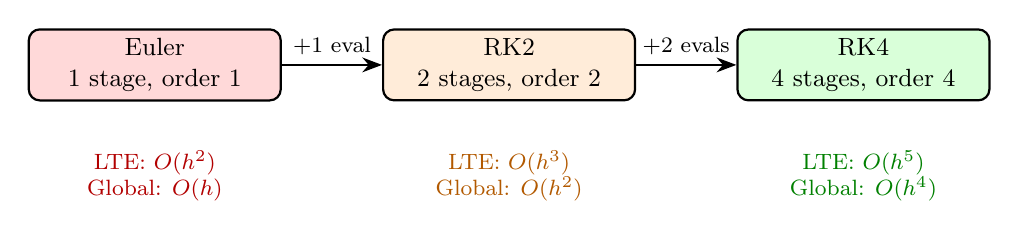
\begin{tikzpicture}[
  box/.style={draw, rounded corners, thick, minimum width=3.2cm, minimum height=0.9cm, 
              align=center, font=\small},
  arr/.style={-{Stealth[length=2.5mm]}, thick}
]
  \node[box, fill=red!15] (euler) at (0, 0) {Euler\\1 stage, order 1};
  \node[box, fill=orange!15] (rk2) at (4.5, 0) {RK2\\2 stages, order 2};
  \node[box, fill=green!15] (rk4) at (9, 0) {RK4\\4 stages, order 4};
  
  \draw[arr] (euler) -- (rk2) node[midway, above, font=\footnotesize] {+1 eval};
  \draw[arr] (rk2) -- (rk4) node[midway, above, font=\footnotesize] {+2 evals};
  
  \node[below=0.5cm, font=\footnotesize, align=center, text=red!70!black] at (euler.south) 
    {LTE: $O(h^2)$\\Global: $O(h)$};
  \node[below=0.5cm, font=\footnotesize, align=center, text=orange!70!black] at (rk2.south) 
    {LTE: $O(h^3)$\\Global: $O(h^2)$};
  \node[below=0.5cm, font=\footnotesize, align=center, text=green!50!black] at (rk4.south) 
    {LTE: $O(h^5)$\\Global: $O(h^4)$};
\end{tikzpicture}
\caption{Summary of the Runge--Kutta hierarchy. Each additional function evaluation ``buys'' more Taylor terms matched.}
\label{fig:summary}
\end{figure}

The derivation has three ingredients:
\begin{enumerate}
  \item Taylor-expand the exact solution $y(t_n + h)$ to the desired order.
  \item Taylor-expand the RK ansatz by recursively expanding each stage.
  \item Match coefficients, yielding algebraic conditions on the Butcher tableau entries. For 4 stages and order 4, there are 8 conditions in 10 unknowns, and the classical choice $c = (0, \tfrac{1}{2}, \tfrac{1}{2}, 1)$ with sequential stage coupling yields the familiar $(1,2,2,1)/6$ weights.
\end{enumerate}


\begin{remark}[Application to backward integration]
\label{rem:rk4_backward}
When integrating backward (as in the robust tax ODE), we set $h < 0$. The RK4 formulas are unchanged---$h$ simply takes negative values, so $k_2$ and $k_3$ evaluate $f$ at $t_n + h/2 < t_n$ and $k_4$ evaluates at $t_n + h < t_n$. The order conditions and error bounds are symmetric in $h$: replacing $h \to -h$ changes the sign of odd-power error terms but preserves the $O(h^5)$ LTE and $O(h^4)$ global error. The only consideration is stability: backward integration reverses the stability properties of the ODE, which is precisely why it is used for the saddle-path problem in Section~\ref{sec:robust_taxation}---the forward-unstable saddle path becomes backward-stable, and numerical errors shrink rather than grow.
\end{remark}
\section{Optimal Control and the Hamiltonian}
\label{app:hamiltonian_primer}

This appendix derives the Hamiltonian optimality conditions used throughout the notes from first principles, via a perturbation (variational) argument. The approach makes explicit the connection to Gâteaux derivatives in function space.

\subsection{The abstract problem}

Consider the continuous-time optimal control problem:
\begin{equation}
\label{eq:abstract_control}
  \max_{u(\cdot),\, x(t_0)} \int_{t_0}^{t_1} L\bigl(t, x(t), u(t)\bigr)\, dt
\end{equation}
subject to the state equation
\begin{equation}
\label{eq:abstract_state}
  \dot{x}(t) = g\bigl(t, x(t), u(t)\bigr),
\end{equation}
where $x(t) \in \R^n$ is the \textbf{state}, $u(t) \in \R^m$ is the \textbf{control}, $L$ is the running payoff, and $g$ governs the state dynamics. The independent choice variables are the control path $u(\cdot)$ and (when the initial state is free) the initial condition $x(t_0)$. The state path $x(t)$ for $t > t_0$ is \emph{not} an independent choice: it is uniquely determined by $u(\cdot)$ and $x(t_0)$ through the ODE \eqref{eq:abstract_state}.

\begin{remark}[Equivalent ``full'' formulation]
\label{rem:full_formulation}
One can equivalently write the problem as $\max_{u(\cdot),\, x(\cdot)}$ subject to the constraint $\dot{x} = g(t,x,u)$, treating the entire state path as a choice variable. This is the formulation that motivates the Hamiltonian: the costate $\lambda(t)$ is the Lagrange multiplier on the state equation at each $t$, and the Hamiltonian $H = L + \lambda^\top g$ is the Lagrangian of this constrained problem. The ``reduced form'' \eqref{eq:abstract_control}--\eqref{eq:abstract_state} and the ``full'' formulation yield identical optimality conditions, but the reduced form makes clear which variables are truly independent.
\end{remark}

The boundary conditions on $x$ depend on the application: $x(t_0)$ may be fixed at a given $x_0$ (drop it from the $\max$), or free (optimized over, as written above). Similarly for $x(t_1)$.

In the taxation problem, the ``time'' variable is the productivity type $z$, the state is utility $\calU(z)$, the control is output $y(z)$, and the state equation is the envelope condition \eqref{eq:IC_law}. Both endpoints $\calU(\zlow)$ and $\calU(\zbar)$ are free: $\calU(\zlow)$ is an independent choice (the planner picks the utility of the bottom type), while $\calU(\zbar)$ is determined by the ODE but unconstrained (the planner does not impose a target for the top type).

\subsection{The Hamiltonian}

Define the \textbf{Hamiltonian}:
\begin{equation}
\label{eq:abstract_H}
  H(t, x, u, \lambda) = L(t, x, u) + \lambda^\top g(t, x, u),
\end{equation}
where $\lambda(t) \in \R^n$ is the \textbf{costate} (adjoint) variable---a Lagrange multiplier on the state equation at each ``time'' $t$.

\subsection{Derivation of the optimality conditions via perturbation}

Suppose $(x^*, u^*)$ is optimal. We present the derivation for the most general case where \emph{both} $x(t_0)$ and $x(t_1)$ are free; the fixed-endpoint cases follow by setting the relevant variation to zero.

Consider a perturbed control $u^\epsilon(t) = u^*(t) + \epsilon\, \delta u(t)$ and a perturbed initial condition $x^\epsilon(t_0) = x^*(t_0) + \epsilon\,\delta x_0$. The perturbed state $x^\epsilon(t)$ satisfies
\[
  \dot{x}^\epsilon = g(t, x^\epsilon, u^\epsilon), \qquad x^\epsilon(t_0) = x^*(t_0) + \epsilon\,\delta x_0.
\]
Define the \textbf{sensitivity} $\delta x(t) = \frac{d x^\epsilon}{d\epsilon}\big|_{\epsilon=0}$, which satisfies the linearized state equation:
\begin{equation}
\label{eq:linearized_state}
  \dot{\delta x} = g_x\, \delta x + g_u\, \delta u, \qquad \delta x(t_0) = \delta x_0.
\end{equation}
When $x(t_0)$ is fixed, $\delta x_0 = 0$ and this reduces to the standard case.

The objective functional is $J(\epsilon) = \int_{t_0}^{t_1} L(t, x^\epsilon, u^\epsilon)\, dt$. Its Gâteaux derivative at $\epsilon = 0$ is
\begin{equation}
\label{eq:gateaux_J}
  \frac{dJ}{d\epsilon}\bigg|_{\epsilon=0} = \int_{t_0}^{t_1} \bigl[L_x\, \delta x + L_u\, \delta u\bigr]\, dt.
\end{equation}
The term $L_x\,\delta x$ is problematic because $\delta x$ depends on $\delta u$ through the linearized state equation \eqref{eq:linearized_state}---it couples the variation at every point. The costate $\lambda$ is introduced precisely to decouple this.

\paragraph{Introducing the costate.}
Since $\dot{x} = g$ is satisfied identically, we can add zero to the objective:
\[
  J = \int_{t_0}^{t_1} \left[L + \lambda^\top\!\bigl(g - \dot{x}\bigr)\right] dt
  = \int_{t_0}^{t_1} \left[H - \lambda^\top \dot{x}\right] dt.
\]
Integrating $\lambda^\top \dot{x}$ by parts: $\int \lambda^\top \dot{x}\, dt = [\lambda^\top x]_{t_0}^{t_1} - \int \dot{\lambda}^\top x\, dt$. Hence
\[
  J = \int_{t_0}^{t_1} \left[H + \dot{\lambda}^\top x\right] dt - \lambda(t_1)^\top x(t_1) + \lambda(t_0)^\top x(t_0).
\]
Now take the Gâteaux derivative, noting that $\delta x(t_0) = \delta x_0$ (which is nonzero when $x(t_0)$ is free):
\begin{align}
  \frac{dJ}{d\epsilon}\bigg|_{\epsilon=0}
  &= \int_{t_0}^{t_1} \bigl[(H_x + \dot{\lambda}^\top)\,\delta x + H_u\,\delta u\bigr]\, dt - \lambda(t_1)^\top \delta x(t_1) + \lambda(t_0)^\top \delta x_0.
  \label{eq:gateaux_augmented}
\end{align}

\paragraph{Choosing $\lambda$ to eliminate $\delta x$.}
If we set
\begin{equation}
\label{eq:abstract_costate}
  \dot{\lambda}(t) = -H_x(t, x^*, u^*, \lambda) \qquad \text{(costate equation)},
\end{equation}
the integral term involving $\delta x$ vanishes. The remaining boundary terms are
\[
  \frac{dJ}{d\epsilon}\bigg|_{\epsilon=0} = \int_{t_0}^{t_1} H_u\,\delta u\, dt + \lambda(t_0)^\top \delta x_0 - \lambda(t_1)^\top \delta x(t_1).
\]
The boundary conditions on $\lambda$ depend on which endpoints are free:
\begin{itemize}[leftmargin=2em]
  \item If $x(t_1)$ is \textbf{free}: $\delta x(t_1)$ is arbitrary, so optimality requires
    \begin{equation}
    \label{eq:abstract_transversality}
      \lambda(t_1) = 0 \qquad \text{(terminal transversality)}.
    \end{equation}
  \item If $x(t_0)$ is \textbf{free}: $\delta x_0$ is arbitrary, so optimality requires
    \begin{equation}
    \label{eq:abstract_transversality_initial}
      \lambda(t_0) = 0 \qquad \text{(initial transversality)}.
    \end{equation}
  \item If $x(t_0)$ is \textbf{fixed} at $x_0$: $\delta x_0 = 0$ and no condition on $\lambda(t_0)$ is needed.
  \item If $x(t_1)$ is \textbf{fixed}: $\delta x(t_1) = 0$ and no condition on $\lambda(t_1)$ is needed.
\end{itemize}
After imposing the relevant boundary conditions, what remains is
\[
  \frac{dJ}{d\epsilon}\bigg|_{\epsilon=0} = \int_{t_0}^{t_1} H_u\,\delta u\, dt.
\]
At an optimum this must be zero for all admissible $\delta u$, giving the \textbf{optimality condition}:
\begin{equation}
\label{eq:abstract_Hu}
  H_u(t, x^*, u^*, \lambda) = 0 \qquad \text{for all } t \in [t_0, t_1].
\end{equation}

\subsection{Summary of the Hamiltonian system}

The three conditions \eqref{eq:abstract_state}, \eqref{eq:abstract_costate}, and \eqref{eq:abstract_Hu} form a two-point boundary value problem. The boundary conditions on $x$ and $\lambda$ are complementary: at each endpoint, either the state is fixed or the costate is zero.

For the case most relevant to the tax problem---both endpoints free---the system is:
\begin{align*}
  \dot{x} &= H_\lambda = g(t, x, u), &\quad& \lambda(t_0) = 0, \\
  \dot{\lambda} &= -H_x, && \lambda(t_1) = 0, \\
  0 &= H_u. &&
\end{align*}
The costate vanishes at both ends because the planner is free to choose both the initial and terminal values of the state. The control $u$ is determined pointwise by the static condition $H_u = 0$.

\begin{remark}[Connection to the tax problem]
In Sections~\ref{sec:hamiltonian}--\ref{sec:formula}, the abstract framework specializes as follows:
\begin{center}
\begin{tabular}{lll}
\textbf{Abstract} & \textbf{Tax problem} & \textbf{Equation} \\
\hline
``Time'' $t$ & Productivity type $z$ & \\
State $x$ & Utility $\calU(z)$ & \\
Control $u$ & Output $y(z)$ & \\
$\dot{x} = g$ & $\calU'(z) = -U_n\,y/z^2$ & \eqref{eq:IC_law} \\
$\dot{\lambda} = -H_x$ & Costate equation & \eqref{eq:costate} \\
$H_u = 0$ & Tax formula & \eqref{eq:Hy} \\
$\lambda(t_0) = \lambda(t_1) = 0$ & $\lambda(\zlow) = \lambda(\zbar) = 0$ & \eqref{eq:boundary}
\end{tabular}
\end{center}
The two-sided boundary condition $\lambda(\zlow) = \lambda(\zbar) = 0$ arises because both endpoints of the state $\calU$ are free: the planner optimizes over the utility of the bottom type (giving $\lambda(\zlow) = 0$ by initial transversality \eqref{eq:abstract_transversality_initial}) and does not impose a target on the utility of the top type (giving $\lambda(\zbar) = 0$ by terminal transversality \eqref{eq:abstract_transversality}).
\end{remark}

\begin{remark}[When is the perturbation approach valid?]
\label{rem:perturbation_validity}
The Gâteaux derivative argument requires:
\begin{enumerate}[label=(\roman*)]
  \item \textbf{Interior optimum:} The optimal control $u^*$ must be interior (no binding inequality constraints on $u$). If the control is constrained, the first-order condition $H_u = 0$ is replaced by the Pontryagin minimum principle, which allows corner solutions.
  \item \textbf{Sufficient smoothness:} The functions $L$, $g$, and the optimal paths $x^*$, $u^*$ must be smooth enough for the integration by parts and the interchange of differentiation and integration to be valid.
  \item \textbf{Sufficiency:} The first-order conditions are necessary but not automatically sufficient. Sufficiency holds under concavity of the Hamiltonian in $(x, u)$ jointly (the Mangasarian sufficient conditions), or can be verified directly by checking second-order conditions.
\end{enumerate}
In the tax problem, condition (i) corresponds to the monotonicity constraint $y'(z) \geq 0$ being non-binding (no bunching). At bunching points, the first-order approach breaks down and one must handle the inequality constraint explicitly. Condition (iii) is ensured by the concavity of $U$ and the single-crossing property.
\end{remark}

\section{Summary of Key Formulas}
\label{app:formulas}

\begin{center}
\renewcommand{\arraystretch}{1.8}
\begin{tabular}{lp{8.5cm}}
\hline\hline
\textbf{Object} & \textbf{Formula} \\
\hline
Envelope condition & $\dfrac{d\calU}{dz} = -U_n\!\left(c, \dfrac{y}{z}\right)\dfrac{y}{z^2}$ \\[8pt]
Frisch elasticity & $\varepsilon^f = \dfrac{U_n}{n\left[U_{nn} - U_{cn}^2/U_{cc}\right]}$ \\[8pt]
Key ratio & $\dfrac{1+\varepsilon^u}{\varepsilon^c} = 1 + n\,\dfrac{U_{nn}+wU_{cn}}{U_n}$ \\[8pt]
General tax formula & $\dfrac{T'}{1-T'} = -\dfrac{1+\varepsilon^u}{\varepsilon^c}\,\dfrac{\lambda(z)}{zf(z)}\,\dfrac{U_c}{\mu}$ \\[8pt]
ABC formula (separable) & $\dfrac{T'}{1-T'} = \dfrac{1+\varepsilon^u}{\varepsilon^c}\,\dfrac{\Psi(z)-\Omega(z)}{z\,\omega(z)}$ \\[8pt]
Top rate (Diamond--Saez) & $T'_{\text{top}} = \dfrac{1}{1+\alpha_y \, e}$ \\[6pt]
\hline\hline
\end{tabular}
\end{center}


%==========================================================================
\section{Mathematical Prerequisites}
\label{app:prerequisites}
%==========================================================================

This appendix collects precise statements of the external
results used in the main text, for ease of reference.

%--------------------------------------------------------------------------
\subsection{The Weierstrass extreme value theorem}
%--------------------------------------------------------------------------

\begin{lemma}[Weierstrass]
\label{lem:weierstrass}
Let $X$ be a nonempty compact topological space and
$f: X \to \R$ an upper semicontinuous function.  Then $f$
attains its supremum: there exists $x^* \in X$ with
$f(x^*) = \sup_{x \in X} f(x)$.

Similarly, if $f$ is lower semicontinuous, then $f$ attains
its infimum.
\end{lemma}

A function $f: X \to \R$ is \textbf{upper semicontinuous}
(u.s.c.) if $\{x : f(x) \geq c\}$ is closed for every
$c \in \R$; equivalently, $\limsup_{x_n \to x} f(x_n)
\leq f(x)$.

We use Weierstrass in Step~5
(Proposition~\ref{prop:existence}): $\calA_q$ is compact
(Helly) and $W$ is continuous (dominated convergence), so
$W$ attains its maximum.


%--------------------------------------------------------------------------
\subsection{Helly's selection theorem}
%--------------------------------------------------------------------------

\begin{lemma}[Helly]
\label{lem:helly}
Let $\{g_n\}_{n=1}^\infty$ be a sequence of functions
$[a,b] \to \R$ that are:
\begin{enumerate}[label=(\roman*)]
\item uniformly bounded: $|g_n(x)| \leq M$ for all
  $n$ and $x$;
\item monotone nondecreasing: $g_n(x) \leq g_n(y)$
  whenever $x \leq y$.
\end{enumerate}
Then there exists a subsequence $\{g_{n_k}\}$ and a
nondecreasing function $g: [a,b] \to \R$ such that
$g_{n_k}(x) \to g(x)$ for every $x \in [a,b]$.
\end{lemma}

We use Helly in Step~3 (Lemma~\ref{lem:Aq_compact}):
the output schedules $q \in \calA_q$ are nondecreasing
and bounded by $\bar q$, so any sequence has a
pointwise convergent subsequence.


%--------------------------------------------------------------------------
\subsection{The dominated convergence theorem}
%--------------------------------------------------------------------------

\begin{lemma}[Lebesgue dominated convergence]
\label{lem:DCT}
Let $(S, \Sigma, \nu)$ be a measure space and
$\{h_n\}_{n=1}^\infty$ a sequence of measurable functions
$S \to \R$.  Suppose:
\begin{enumerate}[label=(\roman*)]
\item $h_n(s) \to h(s)$ for $\nu$-almost every $s$
  (pointwise convergence);
\item there exists an integrable function $H: S \to \R_+$
  with $|h_n(s)| \leq H(s)$ for all $n$ and $\nu$-a.e.\
  $s$ (domination).
\end{enumerate}
Then $h$ is integrable and
$\int_S h_n\,d\nu \to \int_S h\,d\nu$.
\end{lemma}

We use DCT in two places:
\begin{enumerate}[label=(\alph*)]
\item Step~5 (continuity of $W$): if $q_n \to q$
  pointwise, the envelope integral
  $\calU_n(z) = u_0 +
  \int_{\zlow}^z q_n(s)/s^{2+\gamma}\,ds$ converges by
  DCT with dominator $\bar q/s^{2+\gamma}$
  (integrable since $\zlow > 0$).  Then
  $g_{a_n}(z) \to g_a(z)$ pointwise, and
  $e^{-g_{a_n}/\theta} \to e^{-g_a/\theta}$ with
  dominator $e^{(C_r + \|\psi-\mu\|_\infty M)/\theta}$
  (Lemma~\ref{lem:Cr_bound}).
\item Step~5 (integral convergence):
  $\int e^{-g_{a_n}/\theta}f \to
  \int e^{-g_a/\theta}f$ by DCT.
\end{enumerate}


%--------------------------------------------------------------------------
\subsection{H\"{o}lder's inequality}
%--------------------------------------------------------------------------

\begin{lemma}[H\"{o}lder]
\label{lem:holder}
Let $(S, \Sigma, \nu)$ be a measure space, $p, r > 1$ with
$1/p + 1/r = 1$, and $\varphi, \psi \geq 0$ measurable.
Then
\begin{equation}
\label{eq:holder}
  \int_S \varphi\,\psi\,d\nu
  \leq
  \left(\int_S \varphi^p\,d\nu\right)^{\!1/p}
  \left(\int_S \psi^r\,d\nu\right)^{\!1/r}.
\end{equation}
Equality holds if and only if $\varphi^p$ and $\psi^r$
are proportional $\nu$-a.e.
\end{lemma}

We use H\"{o}lder in Step~6
(Proposition~\ref{prop:unique_QL}) with
$\varphi = (e^{-g_1/\theta})^t$,
$\psi = (e^{-g_2/\theta})^{1-t}$,
$p = 1/t$, $r = 1/(1-t)$, and $d\nu = f\,dz$.  The
equality condition ($e^{-g_1/\theta}$ and $e^{-g_2/\theta}$
proportional $f$-a.e.) is used in the case
$q_1(z) = q_2(z)$ for $f$-a.e.\ $z$ but
$u_{0,1} \neq u_{0,2}$: proportionality fails because
$g_1(z) - g_2(z) = (\psi(z)-\mu)(u_{0,1}-u_{0,2})$ is
non-constant when $\psi$ is non-constant
(Assumption~\ref{as:psi}).



%--------------------------------------------------------------------------
\subsection{The taxation principle}
%--------------------------------------------------------------------------

\begin{lemma}[Taxation principle; Hammond 1979, Rochet 1985]
\label{lem:taxation_principle}
Consider an economy with a continuum of agents indexed by
type $z \in \calZ$, preferences $U(c, y/z)$ over
consumption $c$ and earnings $y$, satisfying
Assumptions~1.1--1.2 of the main notes.
\begin{enumerate}[label=(\roman*)]
\item \textbf{From taxes to allocations.}
  Given a tax schedule $T: \R_+ \to \R$ with $T(0) = 0$,
  each type $z$ chooses earnings
  $y(z) \in \arg\max_y\, U(y - T(y),\, y/z)$.  The
  resulting allocation $(c(z), y(z))$ with
  $c(z) = y(z) - T(y(z))$ is incentive-compatible:
  no type prefers the bundle of any other type.
\item \textbf{From allocations to taxes.}
  Given an incentive-compatible allocation $(c(z), y(z))$
  with $y$ nondecreasing, the tax schedule
  $T(y(z)) = y(z) - c(z)$ for $y$ in the range of
  $y(\cdot)$ implements the allocation: each type
  voluntarily chooses its assigned bundle.
\end{enumerate}
The two maps are inverses of each other (on the range of
$y$).  The principle is about household optimization only;
it does not involve the planner's objective or any
properties of the distribution of types.
\end{lemma}


%--------------------------------------------------------------------------
\subsection{The first-order approach}
%--------------------------------------------------------------------------

\begin{lemma}[Sufficiency of the first-order approach;
Mirrlees 1971]
\label{lem:FOA}
Let $U(c, y/z)$ satisfy the single-crossing condition
\begin{equation}
\label{eq:single_crossing_app}
  \frac{\partial}{\partial z}
  \left(-\frac{U_y(c, y/z)}{U_c(c, y/z)}\right) < 0,
\end{equation}
i.e., higher types have a lower marginal rate of
substitution between consumption and earnings.  Then an
allocation $(c(z), y(z))$ is incentive-compatible if and
only if:
\begin{enumerate}[label=(\roman*)]
\item \textbf{Envelope condition:}
  $\calU'(z) = -U_y(c(z), y(z)/z) \cdot y(z)/z^2$
  for a.e.\ $z$, where $\calU(z) = U(c(z), y(z)/z)$.
\item \textbf{Monotonicity:}
  $y(z)$ is nondecreasing.
\end{enumerate}
\end{lemma}

Under separable preferences $U(c,n) = u(c) - v(n)$
with $n = y/z$, the single-crossing condition
\eqref{eq:single_crossing_app} is automatically satisfied
(since $-U_y/U_c = v'(y/z)/(z\,u'(c))$ is decreasing in
$z$ for fixed $(c,y)$).  Under quasilinear isoelastic
preferences, the envelope condition becomes
$\calU'(z) = (y(z)/z)^{1+\gamma}/z = q(z)/z^{2+\gamma}$
(equation~\eqref{eq:q_envelope}).


%--------------------------------------------------------------------------
\subsection{Verification of the envelope hypotheses}
\label{app:envelope_hyp}
%--------------------------------------------------------------------------

Proposition~\ref{prop:envelope} requires three hypotheses
on $g_\alpha(z) = \psi(z)\,\calU_\alpha(z)
+ \mu\,T_\alpha(y_\alpha(z))$
(equation~\eqref{eq:g_alpha_def}), where
$T_\alpha = T + \alpha\,\delta T$ and $y_\alpha(z)$
solves the household's problem under $T_\alpha$.
We trace each condition back to primitives.

\paragraph{Hypothesis (i): differentiability of
$\alpha \mapsto g_\alpha(z)$.}
This requires differentiability of
$\alpha \mapsto y_\alpha(z)$, which follows from the
implicit function theorem (IFT) on the household FOC
\[
  \Phi(\alpha, y)
  = [1 - T'(y) - \alpha\,\delta T'(y)]\,
  U_c(y - T_\alpha(y),\, y/z)
  + \tfrac{1}{z}\,U_n(y - T_\alpha(y),\, y/z) = 0,
\]
provided:
\begin{enumerate}[label=(P\arabic*)]
\item $U \in C^2$, strictly concave (so $\Phi$ is $C^1$
  in $(\alpha, y)$);
\item $T \in C^2$ and $\delta T \in C^1$ in a
  neighborhood of $y_0(z)$;
\item the household SOC holds strictly:
  $\partial_y \Phi(0, y_0(z)) < 0$.
\end{enumerate}
Once $y_\alpha(z)$ is $C^1$ in $\alpha$, the chain
rule gives hypothesis~(i).

For the Saez perturbation, $\delta T'$ is a step
function, so $\delta T \notin C^1$ at the kink points
$y^*$ and $y^* + \varepsilon$.  However, the IFT only
needs to apply at each type's base earnings $y_0(z)$,
and generically only a measure-zero set of types has
$y_0(z) \in \{y^*, y^* + \varepsilon\}$.  So
hypothesis~(i) holds for $f$-a.e.\ $z$.

\paragraph{Hypothesis (ii): finiteness of $Z(\alpha)$.}
On bounded support, $g_\alpha$ is bounded
(Lemma~\ref{lem:Cr_bound} extended to small $\alpha$),
so $e^{-g_\alpha/\theta}$ is bounded and
$Z(\alpha) < \infty$ is automatic.  On unbounded
support, this is a genuine tail condition requiring the
exponential decay from $e^{-g_\alpha/\theta}$ and the
tail decay of $f$ to jointly ensure integrability.

\paragraph{Hypothesis (iii): domination.}
The bound
$|\partial_\alpha g_\alpha|\,e^{-g_\alpha/\theta}
\leq H$ has two parts.

\emph{Bounding $|\partial_\alpha g_\alpha|$.}
By the household envelope theorem,
$\partial_\alpha \calU_\alpha(z)
= -U_c(c_\alpha, y_\alpha/z)\,\delta T(y_\alpha)$,
so
\[
  \partial_\alpha g_\alpha(z)
  = \bigl(\mu - \psi(z)\,U_c\bigr)\,
  \delta T(y_\alpha)
  + \mu\,T'_\alpha(y_\alpha)\,\dot y_\alpha(z),
\]
where $\dot y_\alpha = \partial_\alpha y_\alpha$.
By the IFT,
$\dot y_\alpha = -(\partial_\alpha\Phi)/
(\partial_y\Phi)$.
The numerator involves $\delta T'$ and $\delta T$
(bounded); the denominator is the SOC (bounded away from
zero by (P3)).  So $|\partial_\alpha g_\alpha|$ is
bounded provided:
\begin{enumerate}[label=(P\arabic*),resume]
\item $\psi$ is bounded on $\calZ$;
\item $\delta T$ and $\delta T'$ are bounded on the range
  of earnings;
\item the second derivatives of $U$ are bounded at the
  allocation.
\end{enumerate}

\emph{Bounding $e^{-g_\alpha/\theta}$.}
This requires $g_\alpha(z) \geq -C$ uniformly:
\begin{enumerate}[label=(P\arabic*),resume]
\item $g_\alpha(z)$ is bounded below uniformly in
  $(\alpha, z)$ for $|\alpha| < \alpha_0$.
\end{enumerate}
On compact $\calZ$ with admissibility
($0 \leq T'_\alpha \leq 1$), (P7) follows from bounded
$\psi$, bounded $\calU_\alpha$ (from bounded earnings
and consumption), and bounded $T_\alpha(y_\alpha)$
--- the content of Lemma~\ref{lem:Cr_bound} extended to
small $\alpha$.

\emph{Combining.}
On bounded support,
$|\partial_\alpha g_\alpha| \leq C_1$ and
$e^{-g_\alpha/\theta} \leq C_2$ uniformly, so
$H = C_1 C_2$ is constant and trivially in $L^1(f\,dz)$.

\paragraph{The quasilinear isoelastic case.}
Under $U(c,n) = c - n^{1+\gamma}/(1+\gamma)$:
$U_{cc} = U_{cn} = 0$, the SOC reduces to
$-\gamma n^{\gamma-1}/z^2 < 0$ (automatic for
$\gamma > 0$), income effects vanish, and
$\dot y_0 = -\frac{1}{\gamma}\,
\frac{y_0}{1-T'}\,\delta T'(y_0)$,
which is bounded on compact support.

\paragraph{Unbounded support.}
On $\calZ = [\zlow, \infty)$, the constant-dominator
argument fails.  Hypotheses~(ii) and~(iii) become genuine
tail requirements: the exponential decay from
$e^{-g_\alpha/\theta}$ and the tail decay of $f$ must
jointly overpower the polynomial growth of
$|\partial_\alpha g_\alpha|$ (through $\psi$,
$\delta T(y_\alpha)$, $\dot y_\alpha$).  This must be
verified case by case.

%--------------------------------------------------------------------------
\subsection{Asymptotic notation}
\label{app:asymptotic_notation}
%--------------------------------------------------------------------------

We use three standard asymptotic notations throughout.
Let $f$ and $g$ be real-valued functions with $g(x) > 0$
for all $x$ sufficiently large.

\begin{definition}[Little-$o$]
$f(x) = o(g(x))$ as $x \to \infty$ means
\[
  \lim_{x \to \infty} \frac{f(x)}{g(x)} = 0.
\]
In words: $f$ grows strictly slower than $g$.  The
notation $o(1)$ denotes a quantity that vanishes in the
limit.  For example, $T(y) = \tau\,y + o(y)$ means
$(T(y) - \tau\,y)/y \to 0$, i.e., $T$ is asymptotically
linear with slope $\tau$.
\end{definition}

\begin{definition}[Big-$O$]
$f(x) = O(g(x))$ as $x \to \infty$ means there exist
$C > 0$ and $x_0$ such that $|f(x)| \leq C\,g(x)$ for
all $x \geq x_0$.  In words: $f$ grows no faster than $g$
up to a constant.
\end{definition}
\begin{definition}[Asymptotic equivalence]
  $f(x) \sim g(x)$ as $x \to \infty$ means
  \[
    \lim_{x \to \infty} \frac{f(x)}{g(x)} = 1,
  \]
  or equivalently $f(x) = g(x)\,(1 + o(1))$.  That is,
  the approximation error $f(x) - g(x)$ is negligible
  relative to $g(x)$ itself: $|f - g|/|g| \to 0$.
  For example,
  $\calY(z,\gamma;T) \sim c(\gamma;R)\,z^{\beta}$ means
  that the ratio $\calY(z,\gamma;T)\,/\,(c(\gamma;R)\,z^{\beta})$
  converges to $1$ as $z \to \infty$---the two quantities
  become indistinguishable in percentage terms, even though
  they may differ in absolute level.
  \end{definition}
  
Two properties used repeatedly:
\begin{enumerate}[label=(\roman*)]
  \item If $f \sim g$ and $h \sim k$, then $f/h \sim g/k$
    (ratios of asymptotically equivalent quantities are
    asymptotically equivalent).  This is why
    multiplicative $1 + o(1)$ corrections cancel in the
    ratio $N(y)/D(y)$ in Section~\ref{sec:2D_GHH_top}.
  \item If $f(x) = o(g(x))$, then $e^{f(x)}/e^{g(x)}
    = e^{f(x)-g(x)} \to 0$ whenever $g(x) - f(x) \to
    +\infty$.  This is the mechanism behind the Laplace
    principle in Section~\ref{sec:2D_robust_selection}:
    exponential gaps overwhelm polynomial prefactors.
\end{enumerate}
% appendix_logconcave_facts.tex
%
% Mathematical appendix collecting external results
% used in the uniqueness analysis of Section 12.
% All results are stated without proof.

\subsection*{Appendix: Log-concavity facts used in the
  uniqueness analysis}
\label{app:logconcave}

\addcontentsline{toc}{subsection}{Appendix: Log-concavity
  facts}

This appendix collects the results invoked in the proof of
Proposition~\ref{prop:uniqueness}.  All results are stated
without proof.

\begin{definition}[Log-concavity]
A function $h : \R \to [0,\infty)$ is \emph{log-concave} if
$\log h$ is concave on its support, i.e., for all $x, y$ in
the support and $t \in [0,1]$,
\[
  h(tx + (1-t)y) \geq h(x)^t\,h(y)^{1-t}.
\]
\end{definition}

\begin{theorem}[Closure under multiplication]
\label{fact:closure_mult}
If $h_1$ and $h_2$ are log-concave, then $h_1 \cdot h_2$ is
log-concave.

This is immediate from
$\log(h_1 h_2) = \log h_1 + \log h_2$.
\end{theorem}

\begin{theorem}[Popoviciu's variance inequality {\normalfont (Popoviciu, 1935)}]
\label{fact:popoviciu}
If $X$ is a random variable supported on $[a,b]$, then
$\mathrm{Var}(X) \leq (b - a)^2/4$.
Equality holds if and only if $X$ is a symmetric Bernoulli
on $\{a, b\}$.
\end{theorem}

\begin{theorem}[Log-concave density implies IFR
  {\normalfont (Bagnoli and Bergstrom, 2005, Theorem~2 and Corollary~2)}]
\label{fact:logconcave_IFR}
If $p$ is a log-concave density on $[0,\infty)$ with survival
function $\bar{F}(x) := \int_x^\infty p(t)\,dt$, then $X$ has
\emph{increasing failure rate} (IFR): the hazard rate
$r(x) := p(x)/\bar{F}(x)$ is non-decreasing.
\end{theorem}

\begin{theorem}[IFR implies $\mathrm{CV} \leq 1$
  {\normalfont (standard in reliability theory; see Barlow and Proschan, 1975, Chapter~6)}]
\label{fact:IFR_CV}
If $X$ is IFR with mean $\mu > 0$, then
$\mathrm{Var}(X) \leq \mu^2$, i.e.,
$\mathrm{CV}(X) \leq 1$.
Equality holds only for the exponential distribution.
\end{theorem}

Combining the two theorems above:

\begin{corollary}[Variance bound for log-concave distributions on $\R_+$]
\label{fact:logconcave_CV}
Let $X$ be a non-negative random variable with log-concave
density and finite mean $\mu > 0$.  Then
$\mathrm{CV}(X) \leq 1$.
\end{corollary}

In Proposition~\ref{prop:uniqueness}(b), these results are
applied as follows.  The tilted density
$g_\lambda(e) \propto g(e)\,e^{-\lambda e}$ on
$[e_{\min}, e_{\max}] \subset \R_+$ is log-concave by
Theorem~\ref{fact:closure_mult} (since $g$ is log-concave and
$e \mapsto e^{-\lambda e}$ is log-linear).
The chain
log-concave $\Rightarrow$ IFR
(Theorem~\ref{fact:logconcave_IFR})
$\Rightarrow$ $\mathrm{CV} \leq 1$
(Theorem~\ref{fact:IFR_CV})
then gives $\mathrm{CV}^2(g_\lambda) \leq 1$ for every
$\lambda \geq 0$.

\subsection{Alternative proof for the bound $\mathrm{CV} \leq 1$ for log-concave distributions on $\R_+$}
\begin{proposition}
  Let $X$ be a nonnegative random variable with density $f$ on $[0,\infty)$.
  Assume that $f$ is log-concave on its support. Then
  \[
  \operatorname{Var}(X)\le (\mathbb E X)^2.
  \]
  Equivalently,
  \[
  \mathrm{CV}(X)=\frac{\sqrt{\operatorname{Var}(X)}}{\mathbb E X}\le 1.
  \]
  \end{proposition}
  
  \begin{proof}
  Write $\bar F(x)=\mathbb P(X>x)$ for the survival function, and let
  $I=[a,b)\subseteq [0,\infty)$ be the support of $f$ (so $0\le a<b\le\infty$).
  On $I$, the function $\phi=\log f$ is concave.
  
  We first show that the hazard rate
  \[
  h(x):=\frac{f(x)}{\bar F(x)}
  \]
  is nondecreasing on $I$ (and hence on $[0,\infty)$ if we set $h(x)=0$ for $x<a$).
  
  Fix $a\le x<y<b$, and let $u\in[0,b-y)$. Set
  \[
  \theta=\frac{u}{y-x+u}\in[0,1].
  \]
  Then
  \[
  y=\theta x+(1-\theta)(y+u),
  \qquad
  x+u=(1-\theta)x+\theta(y+u).
  \]
  By concavity of $\phi$,
  \[
  \phi(y)\ge \theta \phi(x)+(1-\theta)\phi(y+u),
  \]
  and
  \[
  \phi(x+u)\ge (1-\theta)\phi(x)+\theta\phi(y+u).
  \]
  Adding these two inequalities gives
  \[
  \phi(y)+\phi(x+u)\ge \phi(x)+\phi(y+u),
  \]
  hence
  \[
  f(x)\,f(y+u)\le f(y)\,f(x+u).
  \]
  Integrating in $u$ over $[0,b-y)$ yields
  \[
  f(x)\bar F(y)\le f(y)\bar F(x),
  \]
  that is,
  \[
  h(x)\le h(y).
  \]
  So $h$ is nondecreasing.
  
  Next we show that $\bar F$ is submultiplicative:
  \[
  \bar F(x+y)\le \bar F(x)\bar F(y)
  \qquad\text{for all }x,y\ge0.
  \]
  Indeed, if $x+y\ge b$, then $\bar F(x+y)=0$ and there is nothing to prove.
  So assume $x+y<b$. Since $\bar F$ is absolutely continuous and
  $\bar F'(t)=-f(t)$ a.e. on $[0,b)$, we have
  \[
  (\log \bar F)'(t)=\frac{\bar F'(t)}{\bar F(t)}=-h(t)
  \qquad\text{a.e.}
  \]
  Therefore
  \[
  \log \bar F(x+y)-\log \bar F(x)
  =
  -\int_x^{x+y} h(s)\,ds
  \le
  -\int_0^y h(s)\,ds
  =
  \log \bar F(y),
  \]
  because $h$ is nondecreasing. Exponentiating gives
  \[
  \bar F(x+y)\le \bar F(x)\bar F(y).
  \]
  
  In particular, choose $r>0$ with $\bar F(r)<1$. Then
  \[
  \bar F(nr)\le \bar F(r)^n,
  \]
  so $\bar F$ decays at least exponentially on a lattice, and hence
  $\mathbb E X<\infty$. Thus the standard tail identities apply:
  \[
  \mathbb E X=\int_0^\infty \bar F(x)\,dx,
  \qquad
  \mathbb E X^2 = 2\int_0^\infty x\,\bar F(x)\,dx.
  \]
  
  Now, by submultiplicativity of $\bar F$,
  \[
  x\,\bar F(x)=\int_0^x \bar F(x)\,du
  \le
  \int_0^x \bar F(u)\bar F(x-u)\,du.
  \]
  Integrating over $x\in[0,\infty)$ and applying Fubini,
  \[
  \frac{\mathbb E X^2}{2}
  =
  \int_0^\infty x\,\bar F(x)\,dx
  \le
  \int_0^\infty\int_0^x \bar F(u)\bar F(x-u)\,du\,dx
  =
  \left(\int_0^\infty \bar F(u)\,du\right)^2
  =
  (\mathbb E X)^2.
  \]
  Hence
  \[
  \mathbb E X^2\le 2(\mathbb E X)^2,
  \]
  and therefore
  \[
  \operatorname{Var}(X)
  =
  \mathbb E X^2-(\mathbb E X)^2
  \le
  (\mathbb E X)^2.
  \]
  This is exactly $\mathrm{CV}(X)\le 1$.
  \end{proof}

\paragraph{References for this appendix.}

\begin{itemize}
  \item Bagnoli, M.\ and Bergstrom, T.\ (2005).
    ``Log-concave probability and its applications.''
    \emph{Economic Theory}, 26(2), 445--469.
  \item Barlow, R.E.\ and Proschan, F.\ (1975).
    \emph{Statistical Theory of Reliability and Life Testing:
    Probability Models.}
    Holt, Rinehart and Winston, New York.
  \item Popoviciu, T.\ (1935).
    ``Sur les \'equations alg\'ebriques ayant toutes leurs
    racines r\'eelles.''
    \emph{Mathematica (Cluj)}, 9, 129--145.
\end{itemize}


\end{document}
